\subsection{3bV validation regions}
The pre-fit and post-fit plots in validation region 3bV is shown in Figures \ref{validation_plots} from the background-only unblinded-data fits. These fits are performed for GNN Distribution for the mass point $m_{H}=400$ GeV including all systematics. From the plots, it can be inferred that there is a good postfit agreement. The lowest $\chi^2$ for 1L channel is 7\% while for 2LOS channel, it is 16\%.

\begin{figure}[htpb!]
        \begin{subfigure}{\textwidth}
        \begin{center} \setlength{\tabcolsep}{2.5pt}\footnotesize
        \begin{tabular}{cccc}
        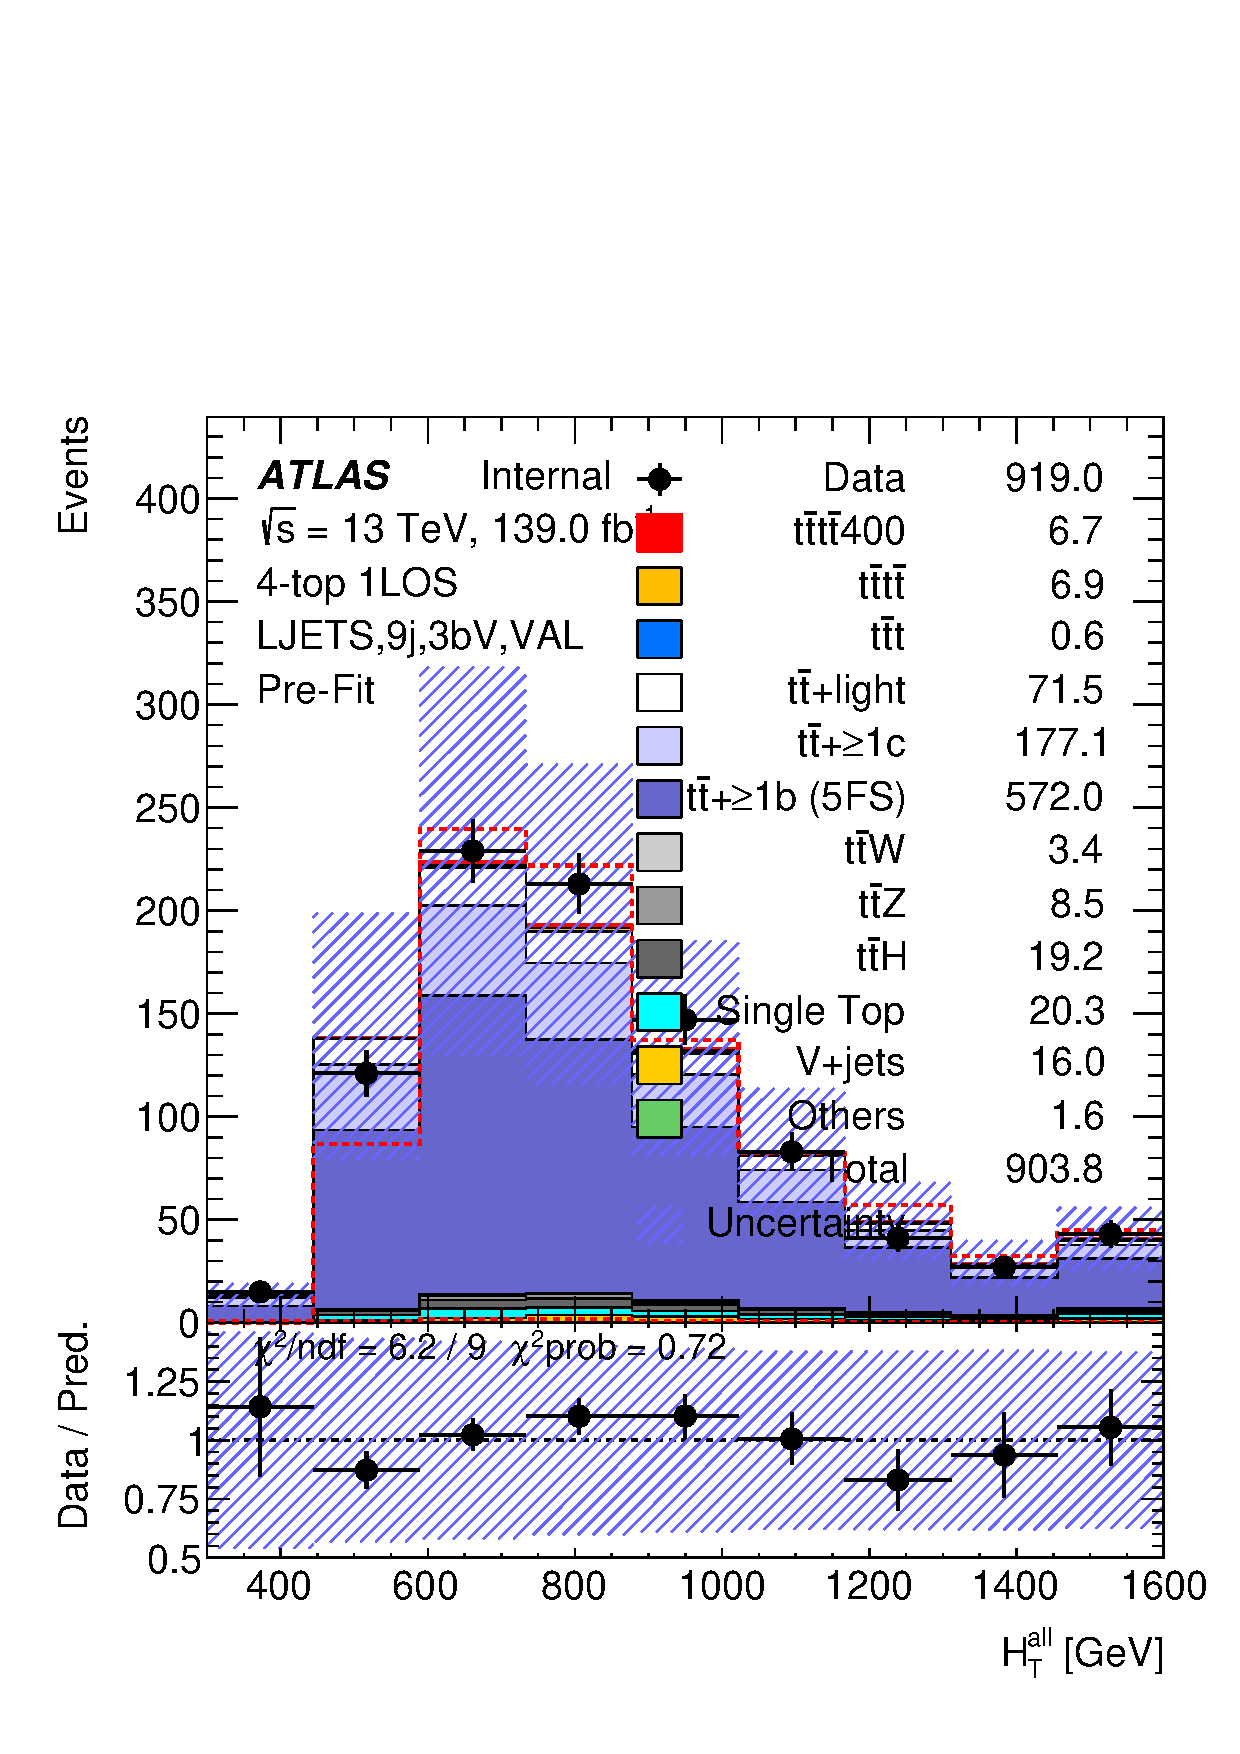
\includegraphics[width=0.23 \textwidth]{figures/fits/GNN/400/all/data_unblindedBonly/Plots/val_ljets_9j3bV_HT_all.pdf} &
        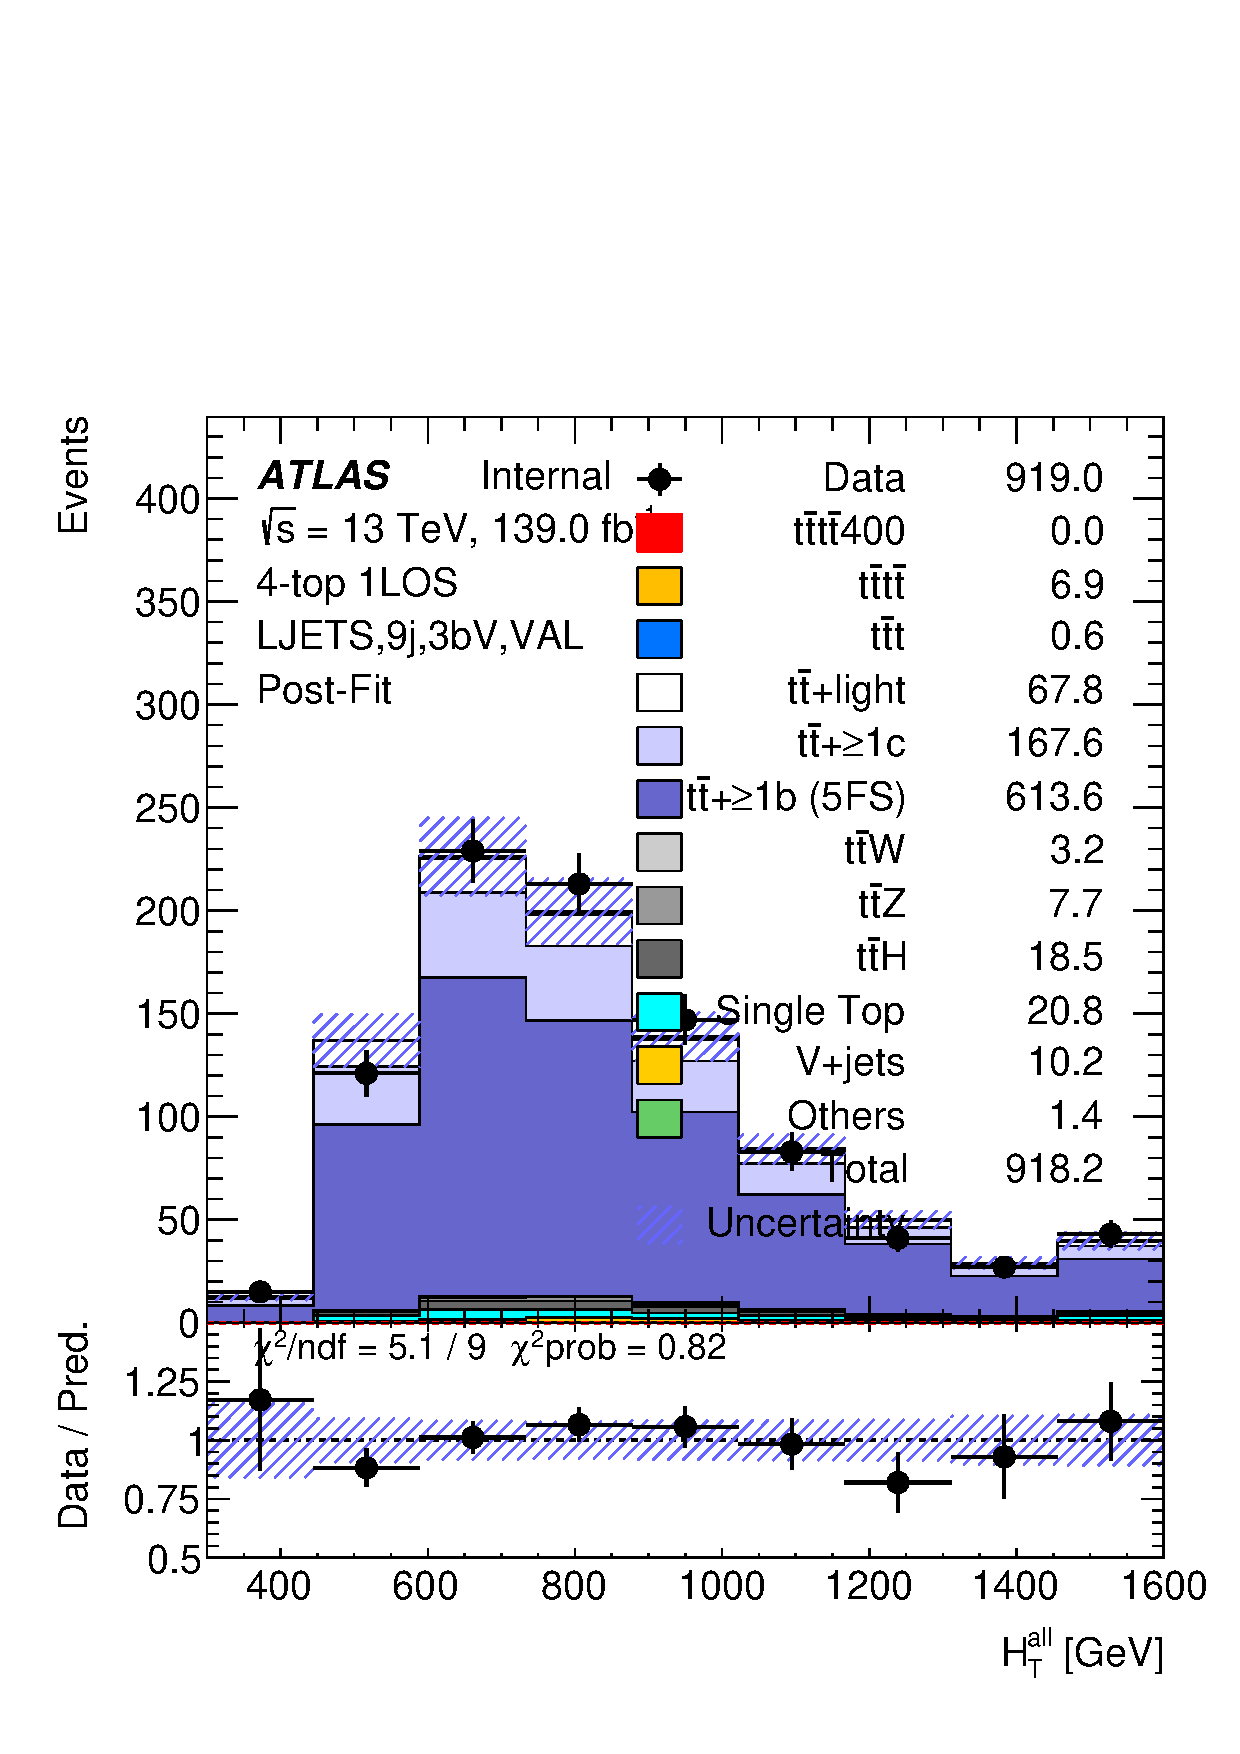
\includegraphics[width=0.23 \textwidth]{figures/fits/GNN/400/all/data_unblindedBonly/Plots/val_ljets_9j3bV_HT_all_postFit.pdf} &
        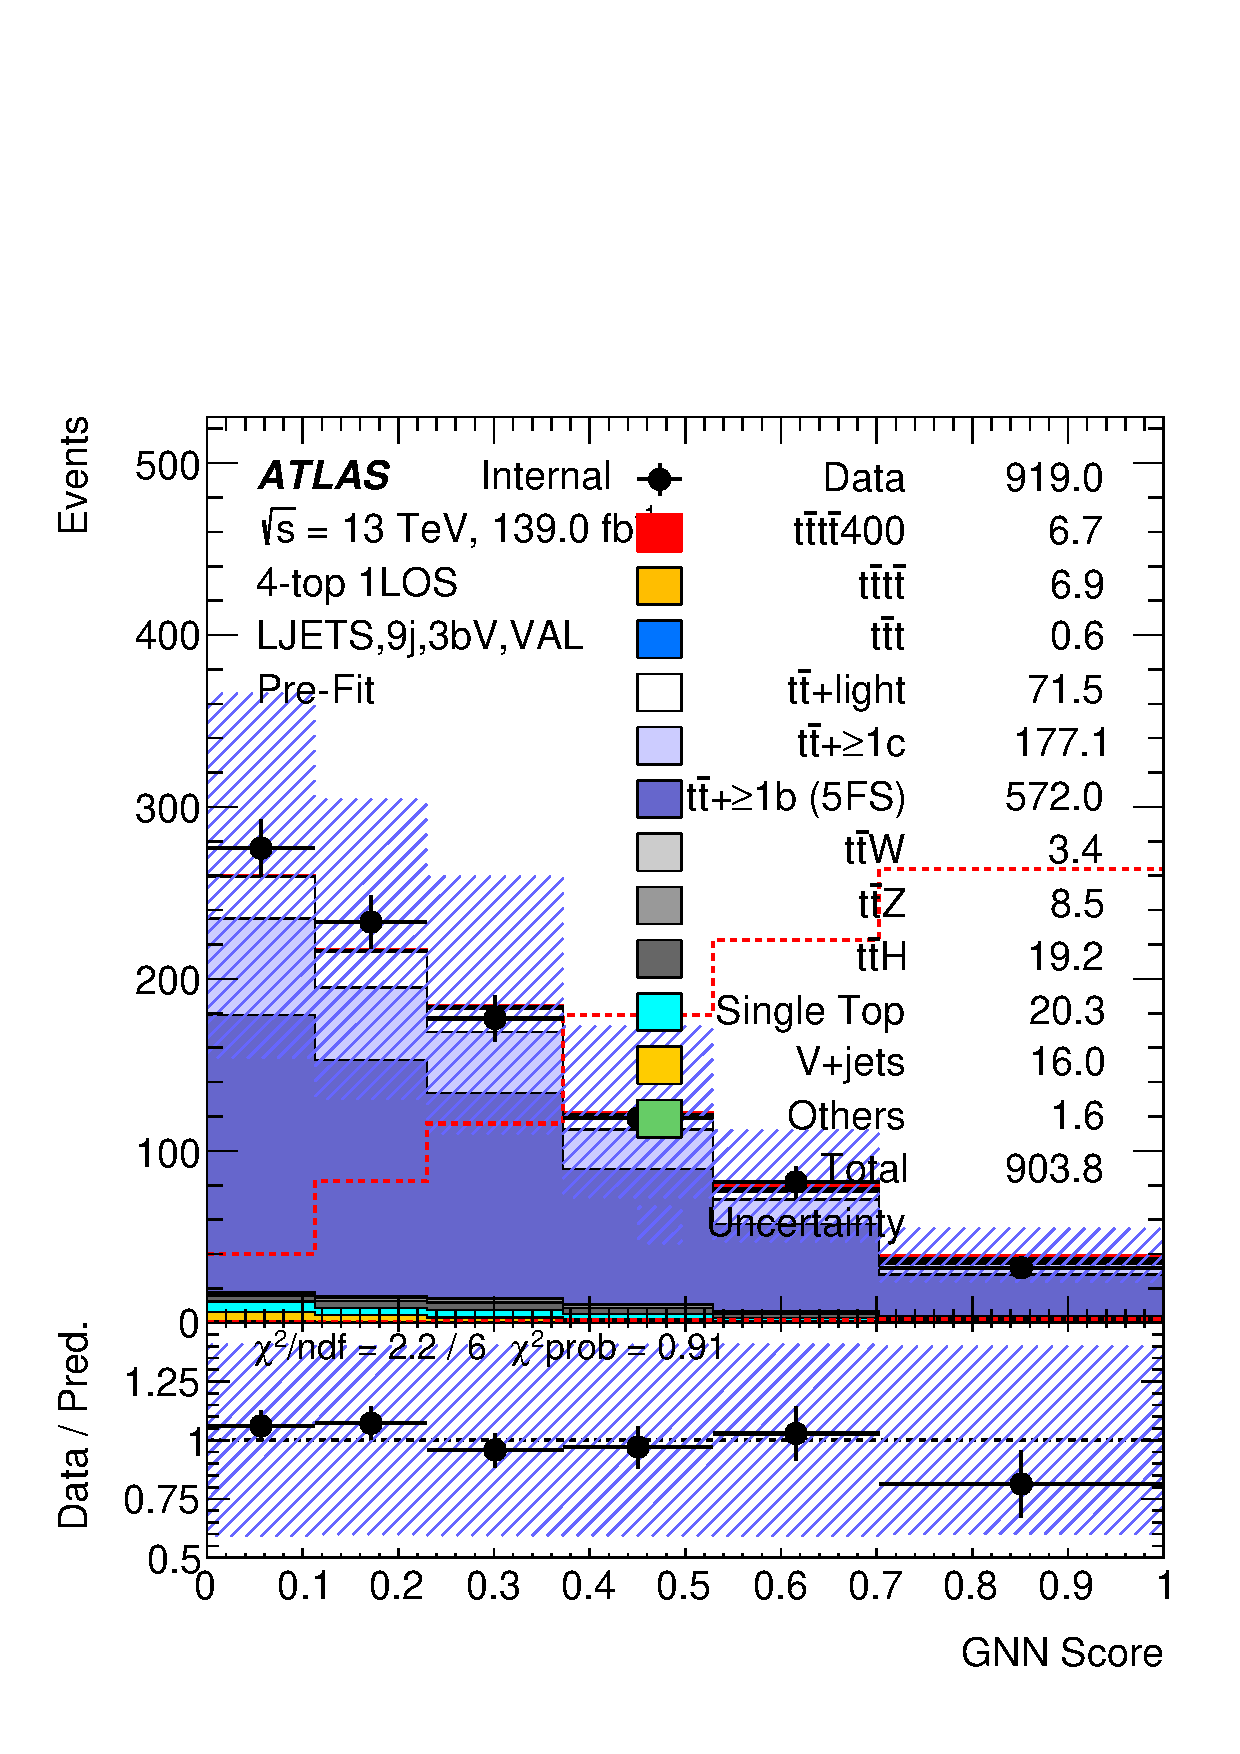
\includegraphics[width=0.23 \textwidth]{figures/fits/GNN/400/all/data_unblindedBonly/Plots/val_ljets_9j3bV_MVA.pdf} &
        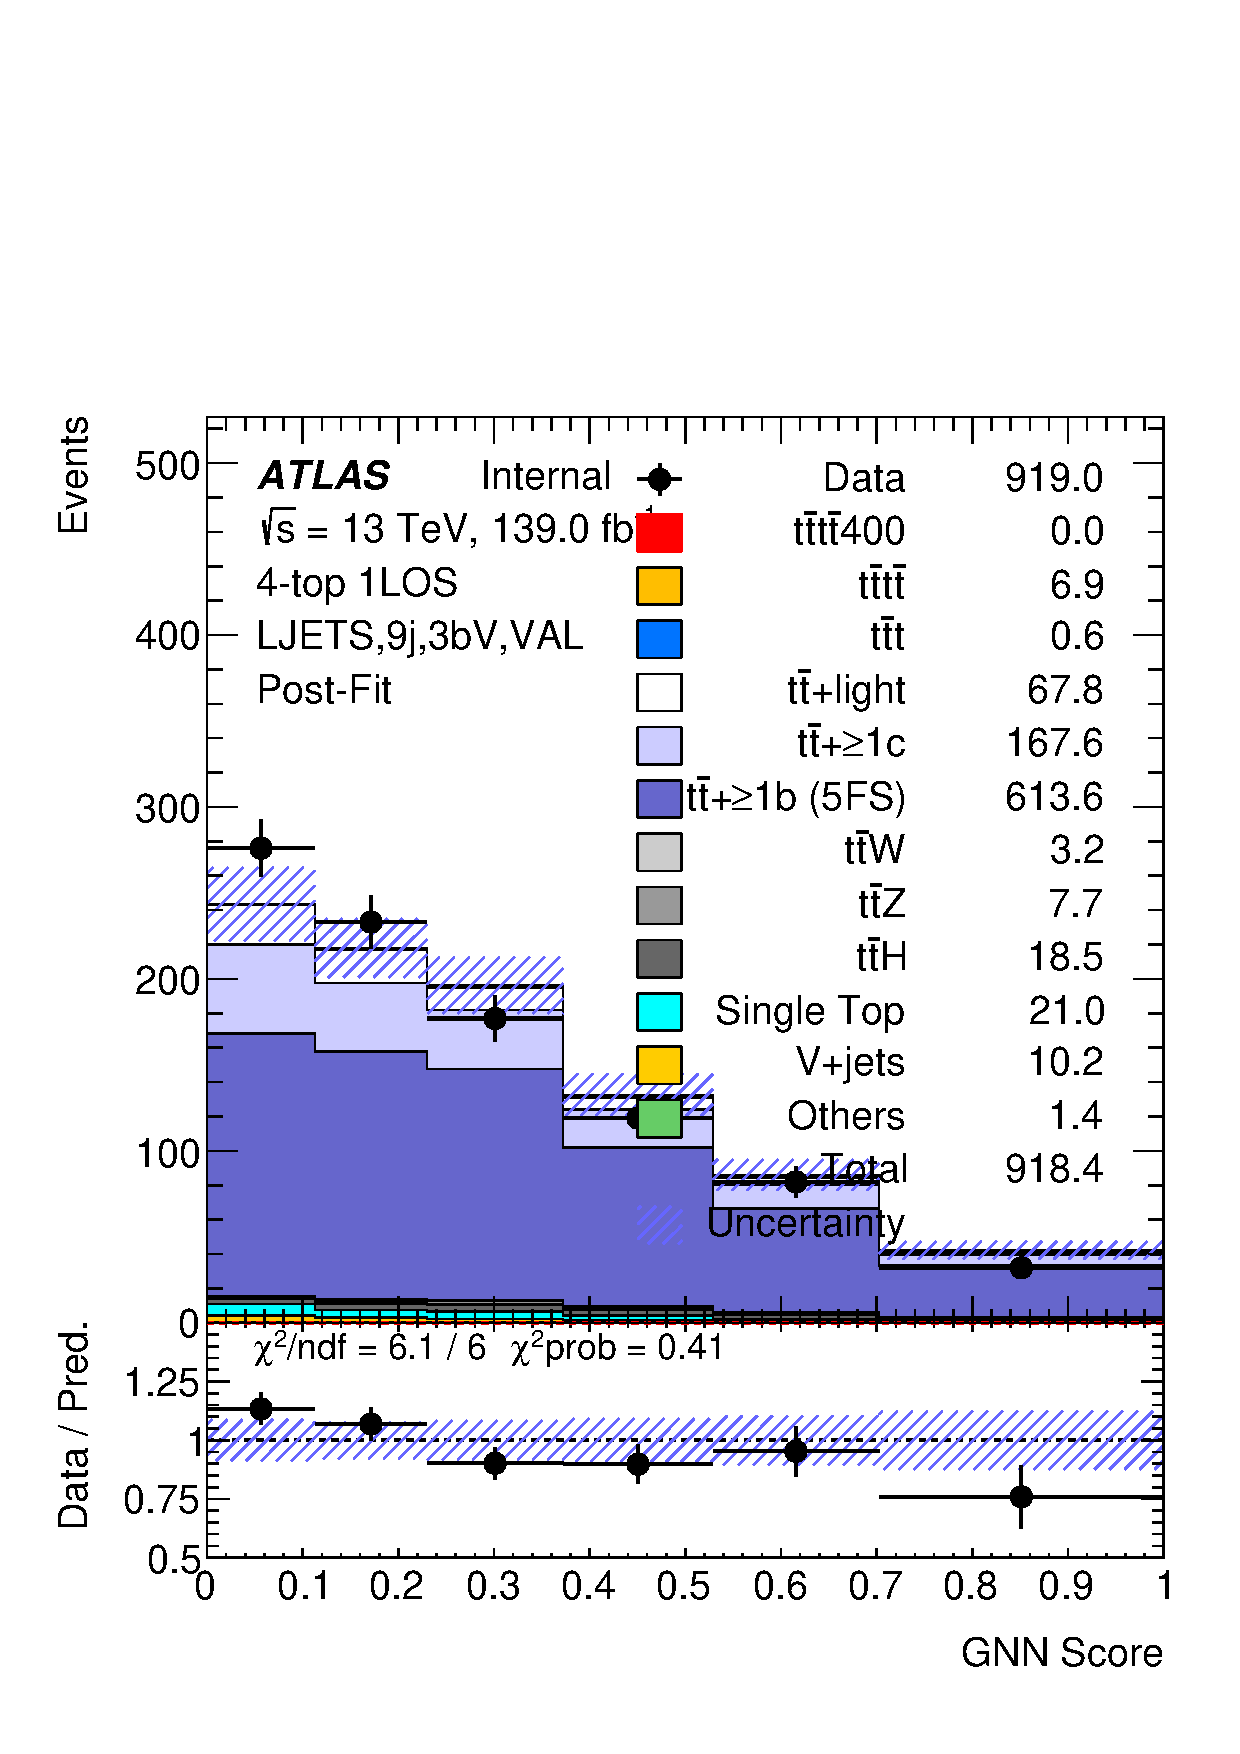
\includegraphics[width=0.23 \textwidth]{figures/fits/GNN/400/all/data_unblindedBonly/Plots/val_ljets_9j3bV_MVA_postFit.pdf}\\

        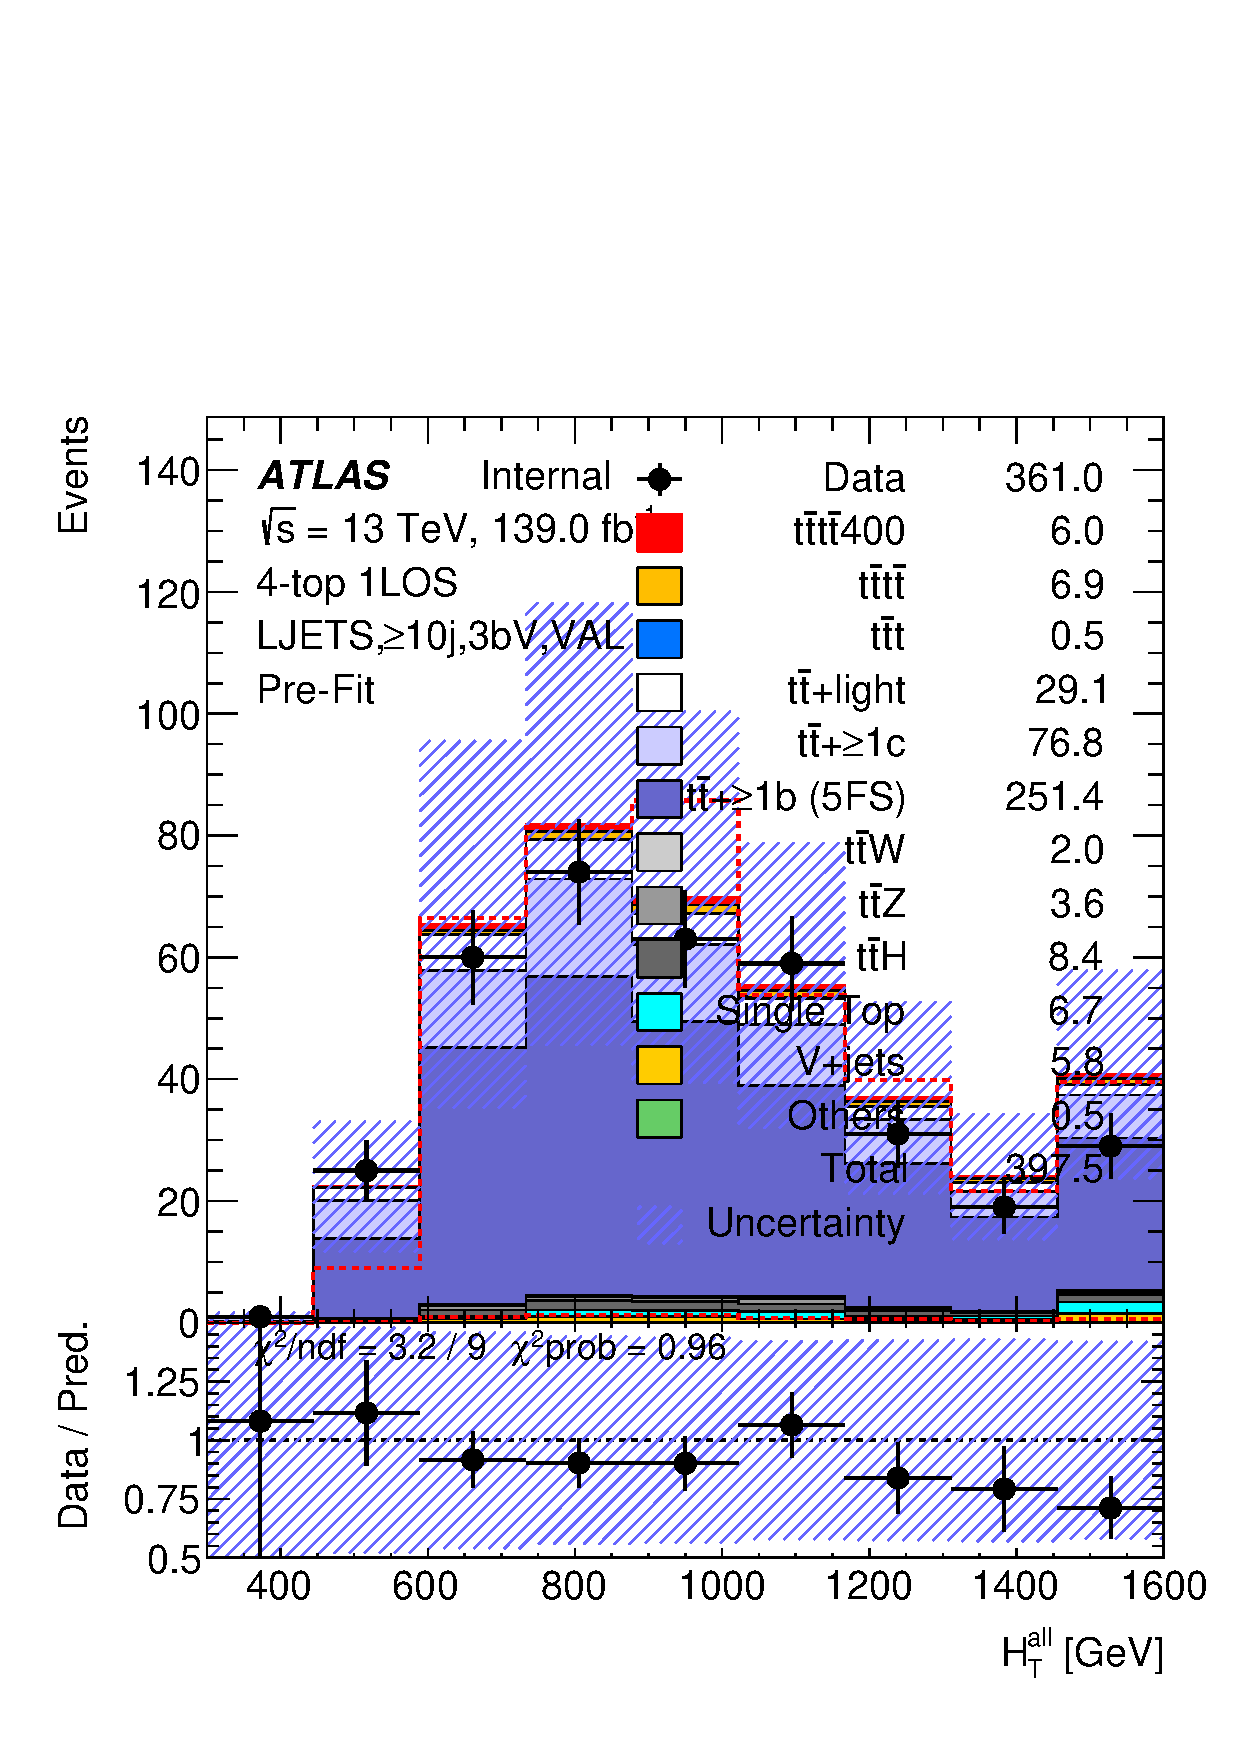
\includegraphics[width=0.23 \textwidth]{figures/fits/GNN/400/all/data_unblindedBonly/Plots/val_ljets_ge10j3bV_HT_all.pdf} &
        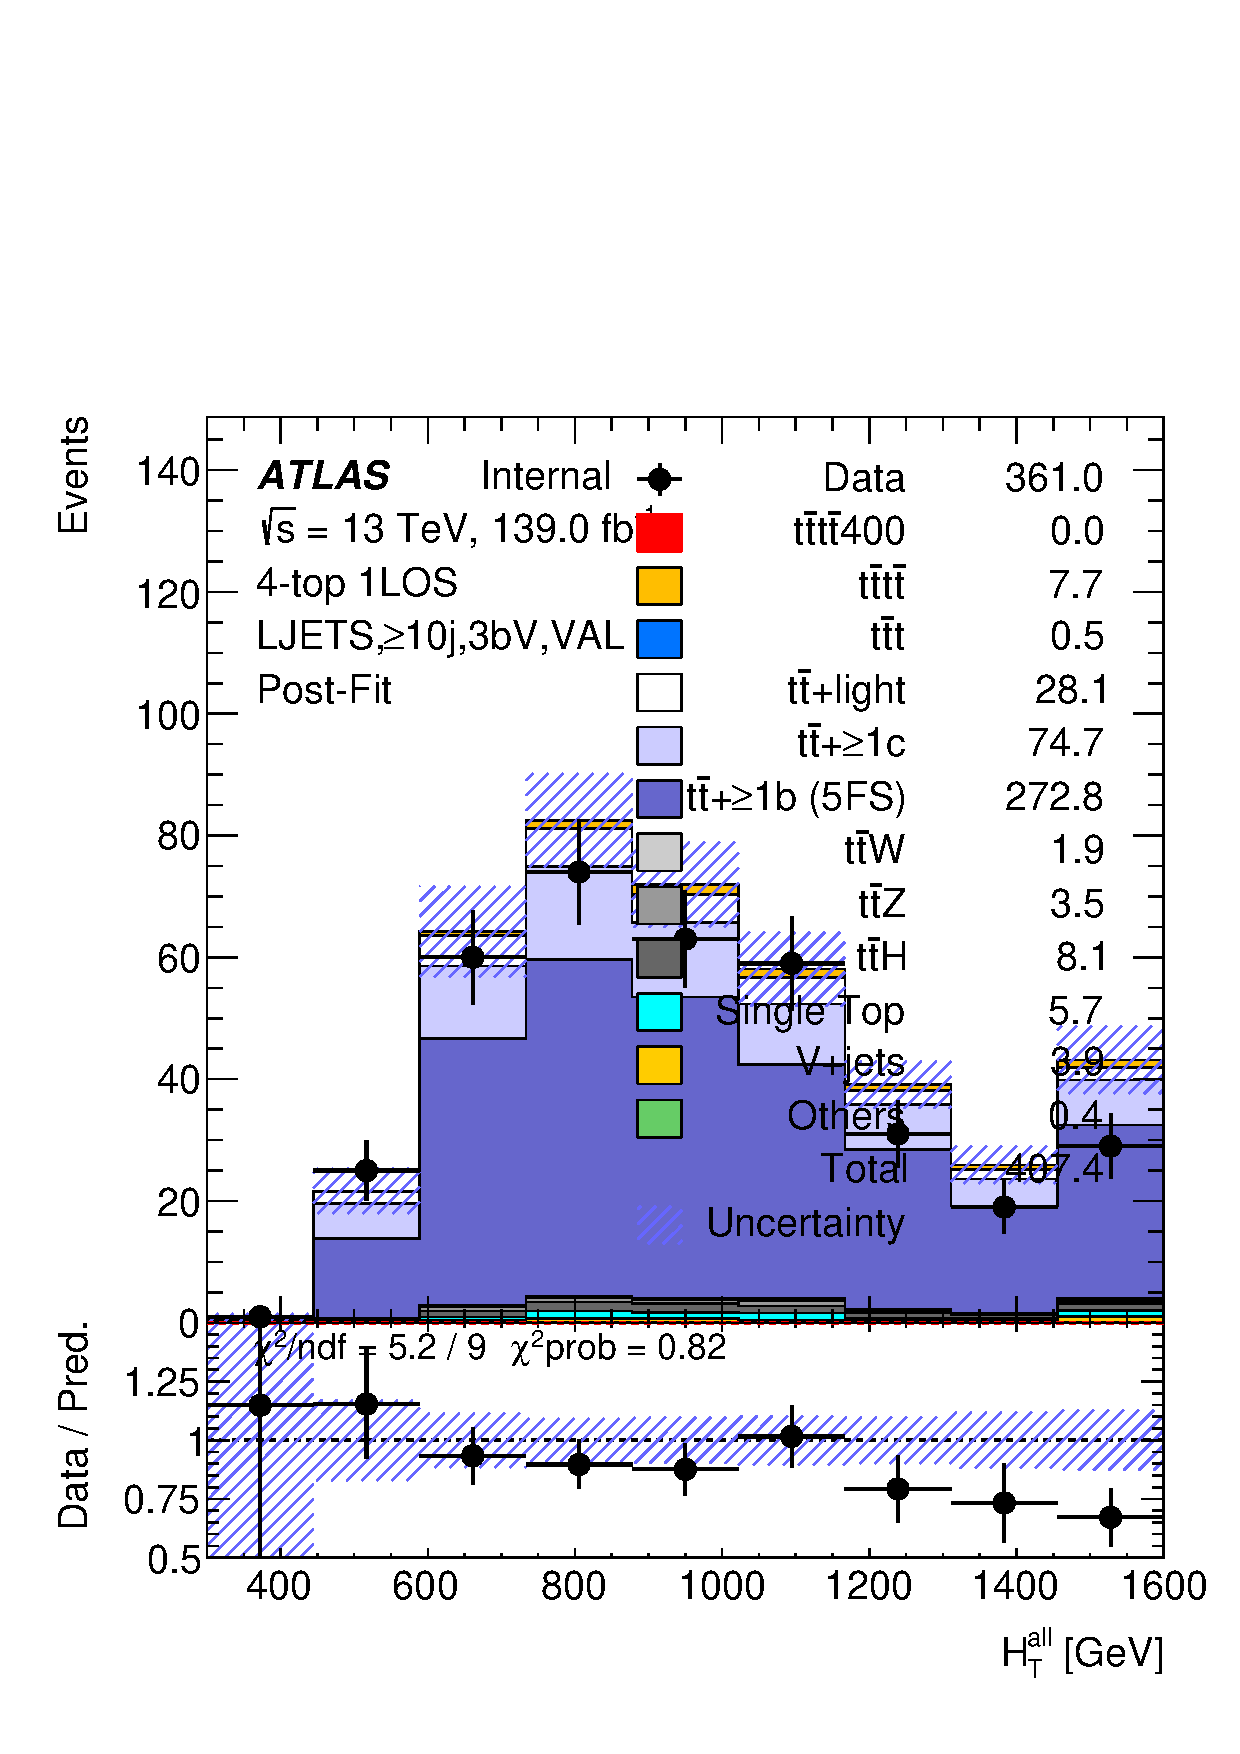
\includegraphics[width=0.23 \textwidth]{figures/fits/GNN/400/all/data_unblindedBonly/Plots/val_ljets_ge10j3bV_HT_all_postFit.pdf} &
        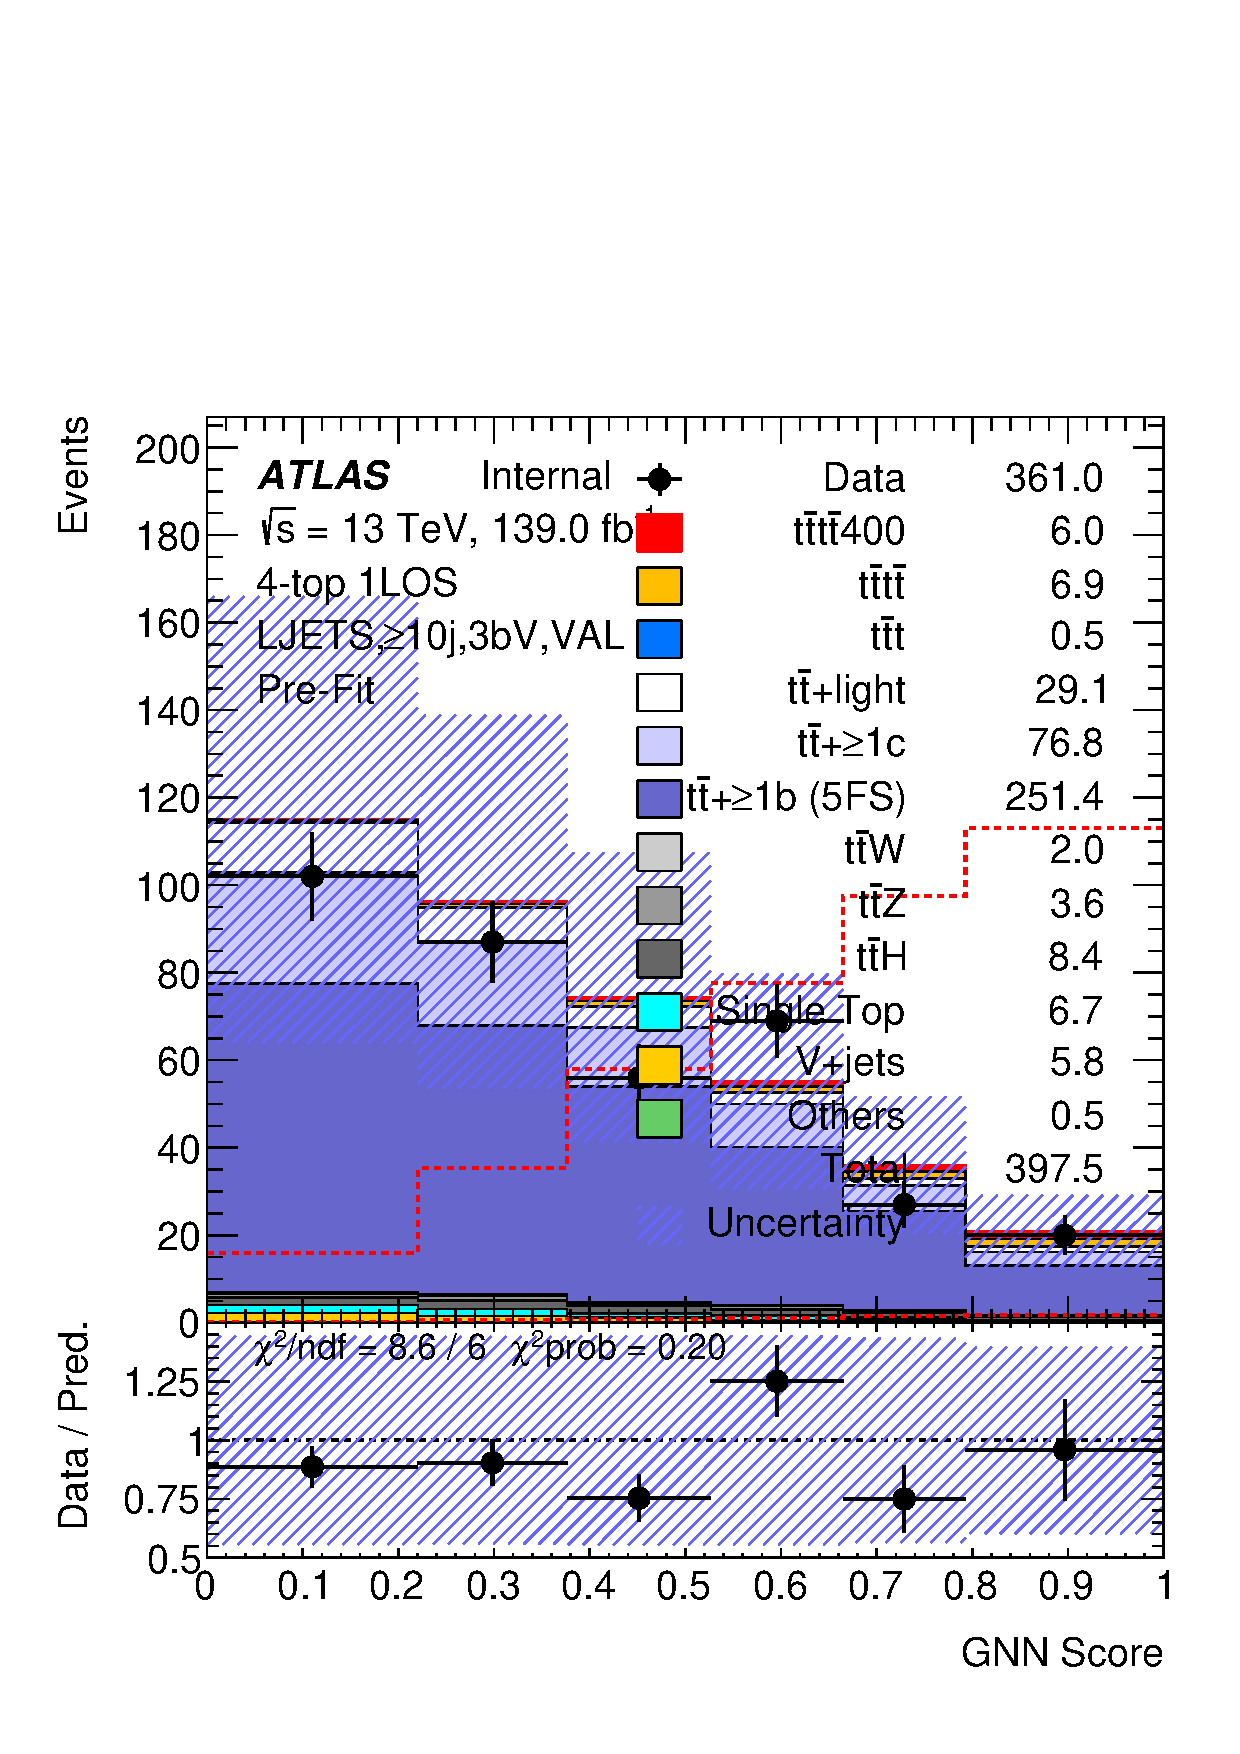
\includegraphics[width=0.23 \textwidth]{figures/fits/GNN/400/all/data_unblindedBonly/Plots/val_ljets_ge10j3bV_MVA.pdf} &
        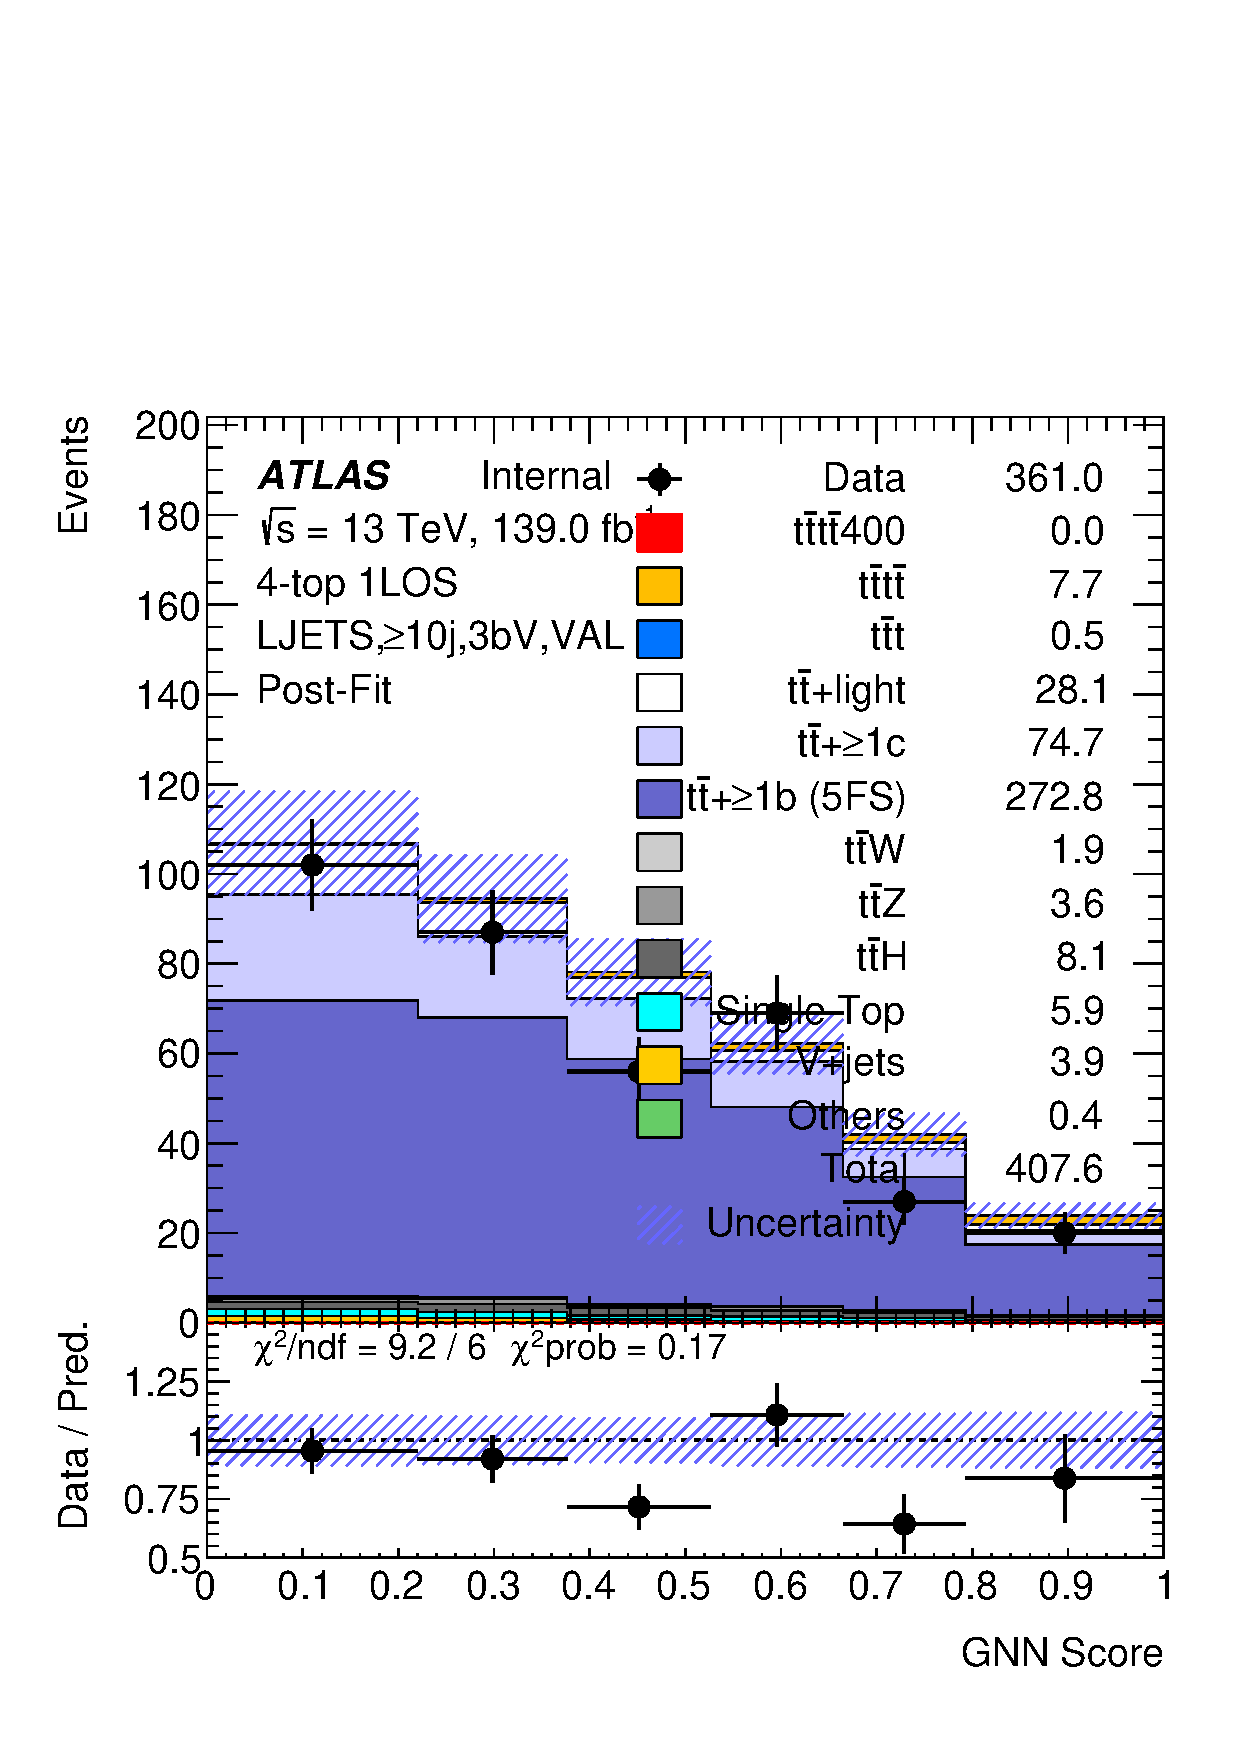
\includegraphics[width=0.23 \textwidth]{figures/fits/GNN/400/all/data_unblindedBonly/Plots/val_ljets_ge10j3bV_MVA_postFit.pdf} \\
        \end{tabular}
        \end{center}
        \caption{\label{val_region_fig1}Pre-fit and Post-fit distribution in 3bV 1L validation regions. First row shows ljets(9j3bV) region and second row shows ljets(ge10j3bV) region.}
        \end{subfigure}
        \bigskip

        \begin{subfigure}{\textwidth}
        \begin{center} \setlength{\tabcolsep}{2.5pt}\footnotesize
        \begin{tabular}{cccc}
        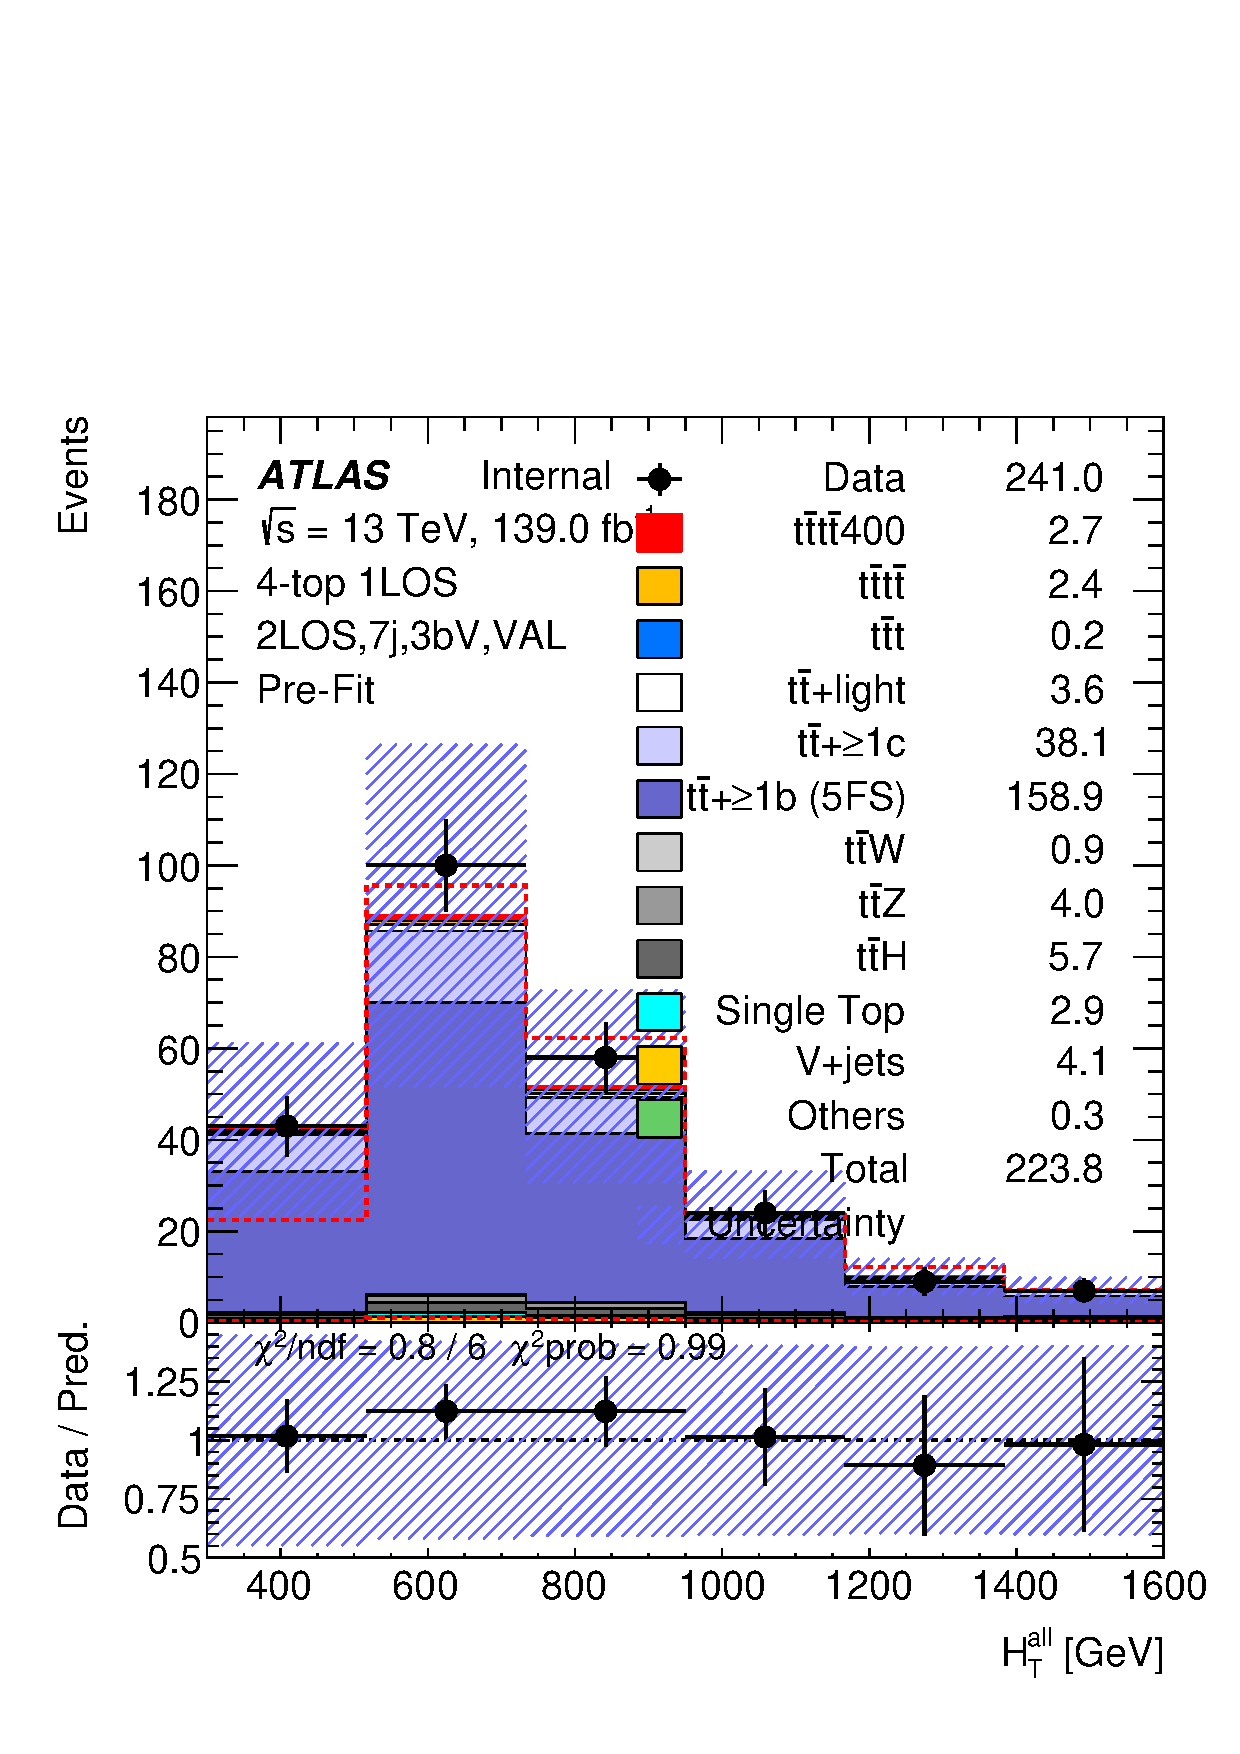
\includegraphics[width=0.23 \textwidth]{figures/fits/GNN/400/all/data_unblindedBonly/Plots/val_os2l_7j3bV_HT_all.pdf} &
        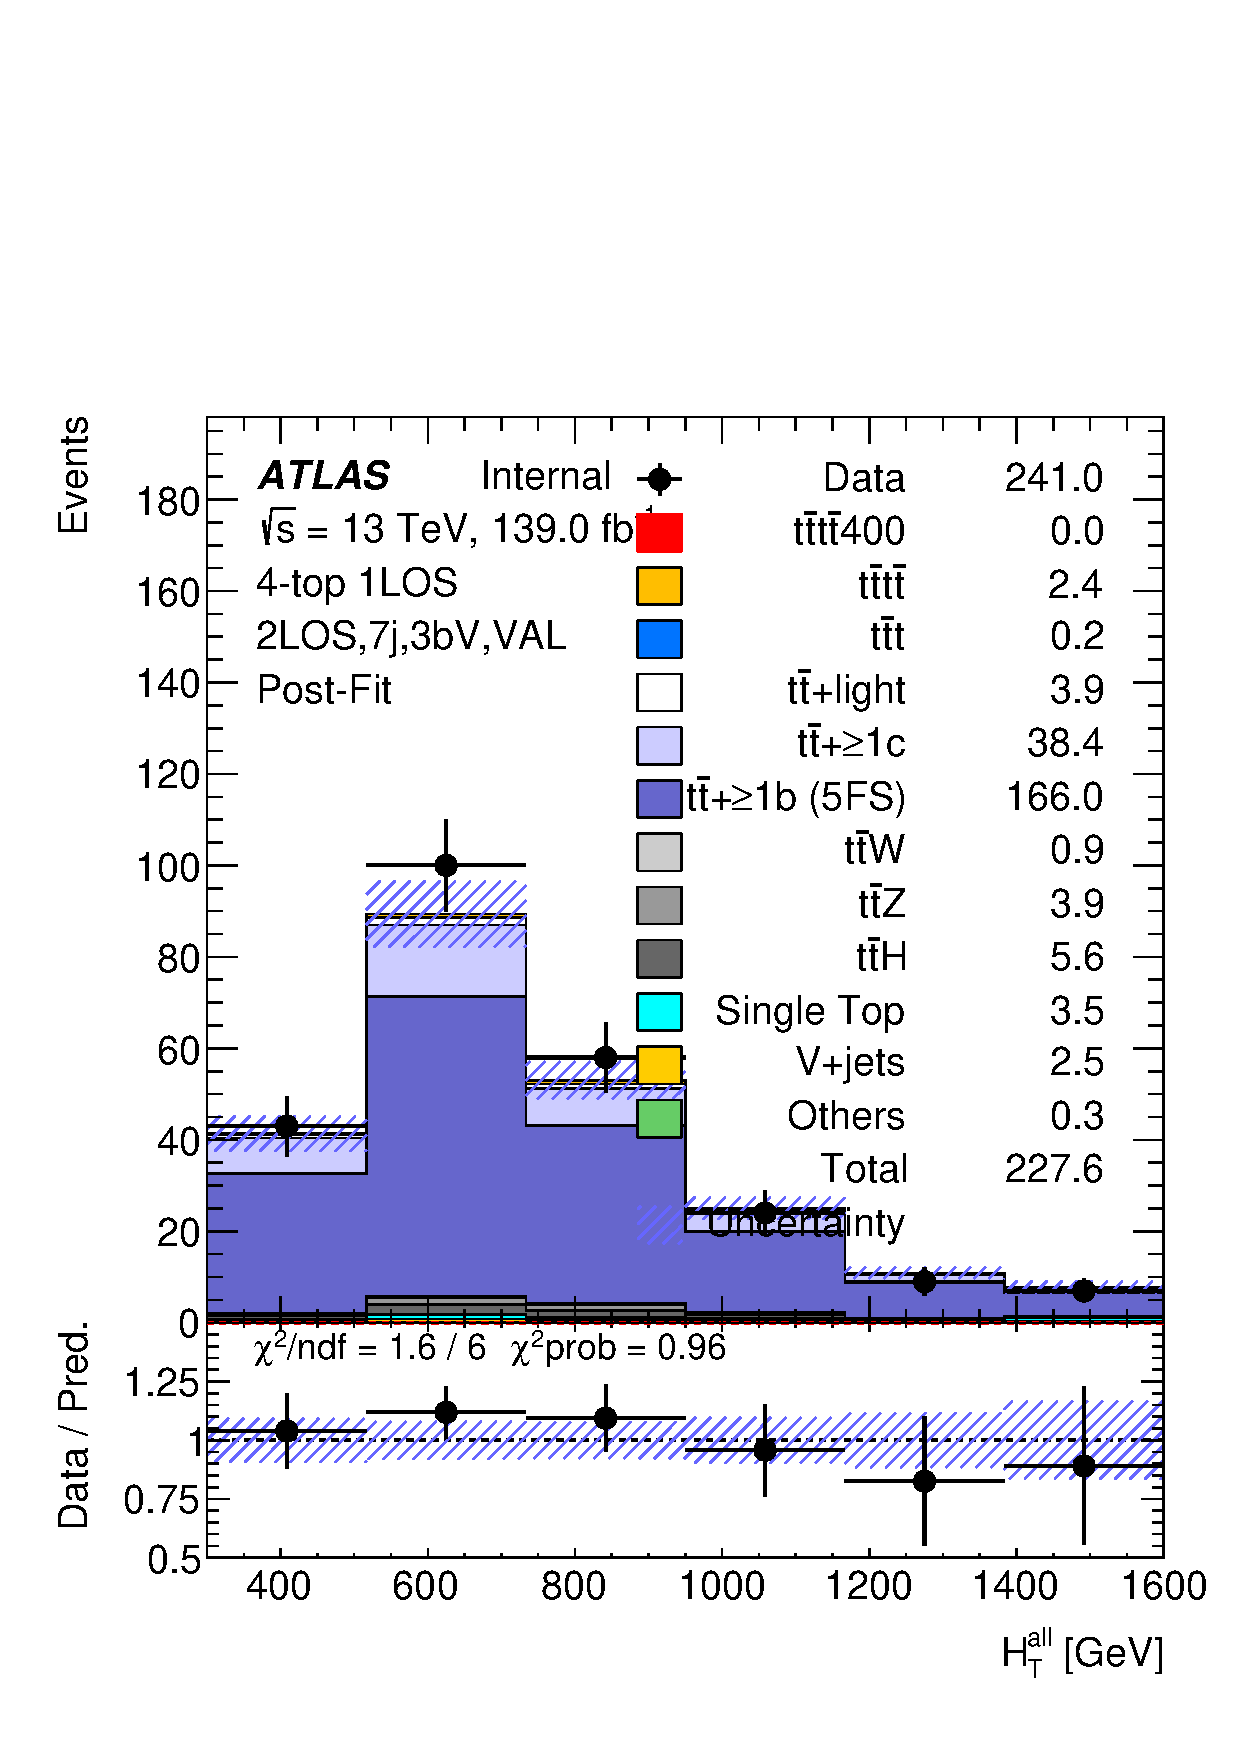
\includegraphics[width=0.23 \textwidth]{figures/fits/GNN/400/all/data_unblindedBonly/Plots/val_os2l_7j3bV_HT_all_postFit.pdf} &
        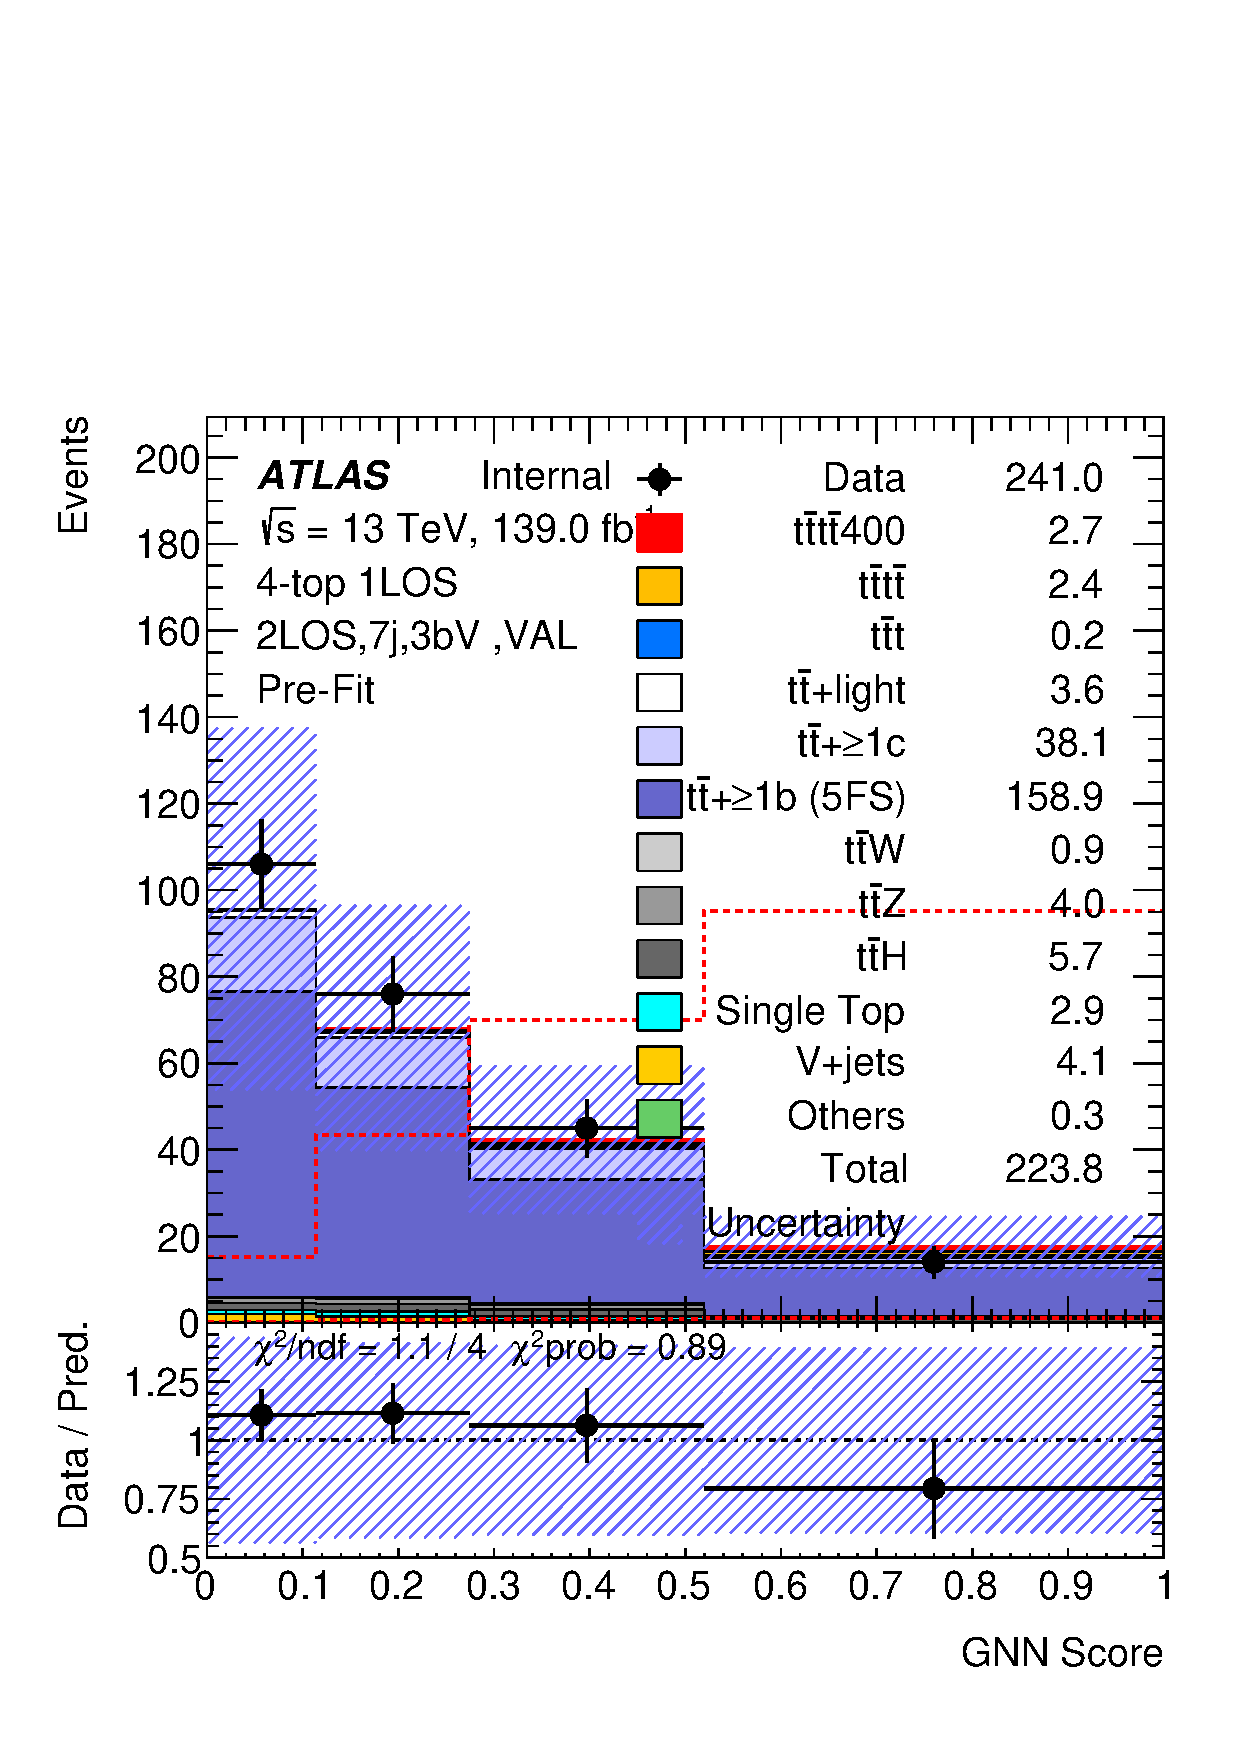
\includegraphics[width=0.23 \textwidth]{figures/fits/GNN/400/all/data_unblindedBonly/Plots/val_os2l_7j3bV_MVA.pdf} &
        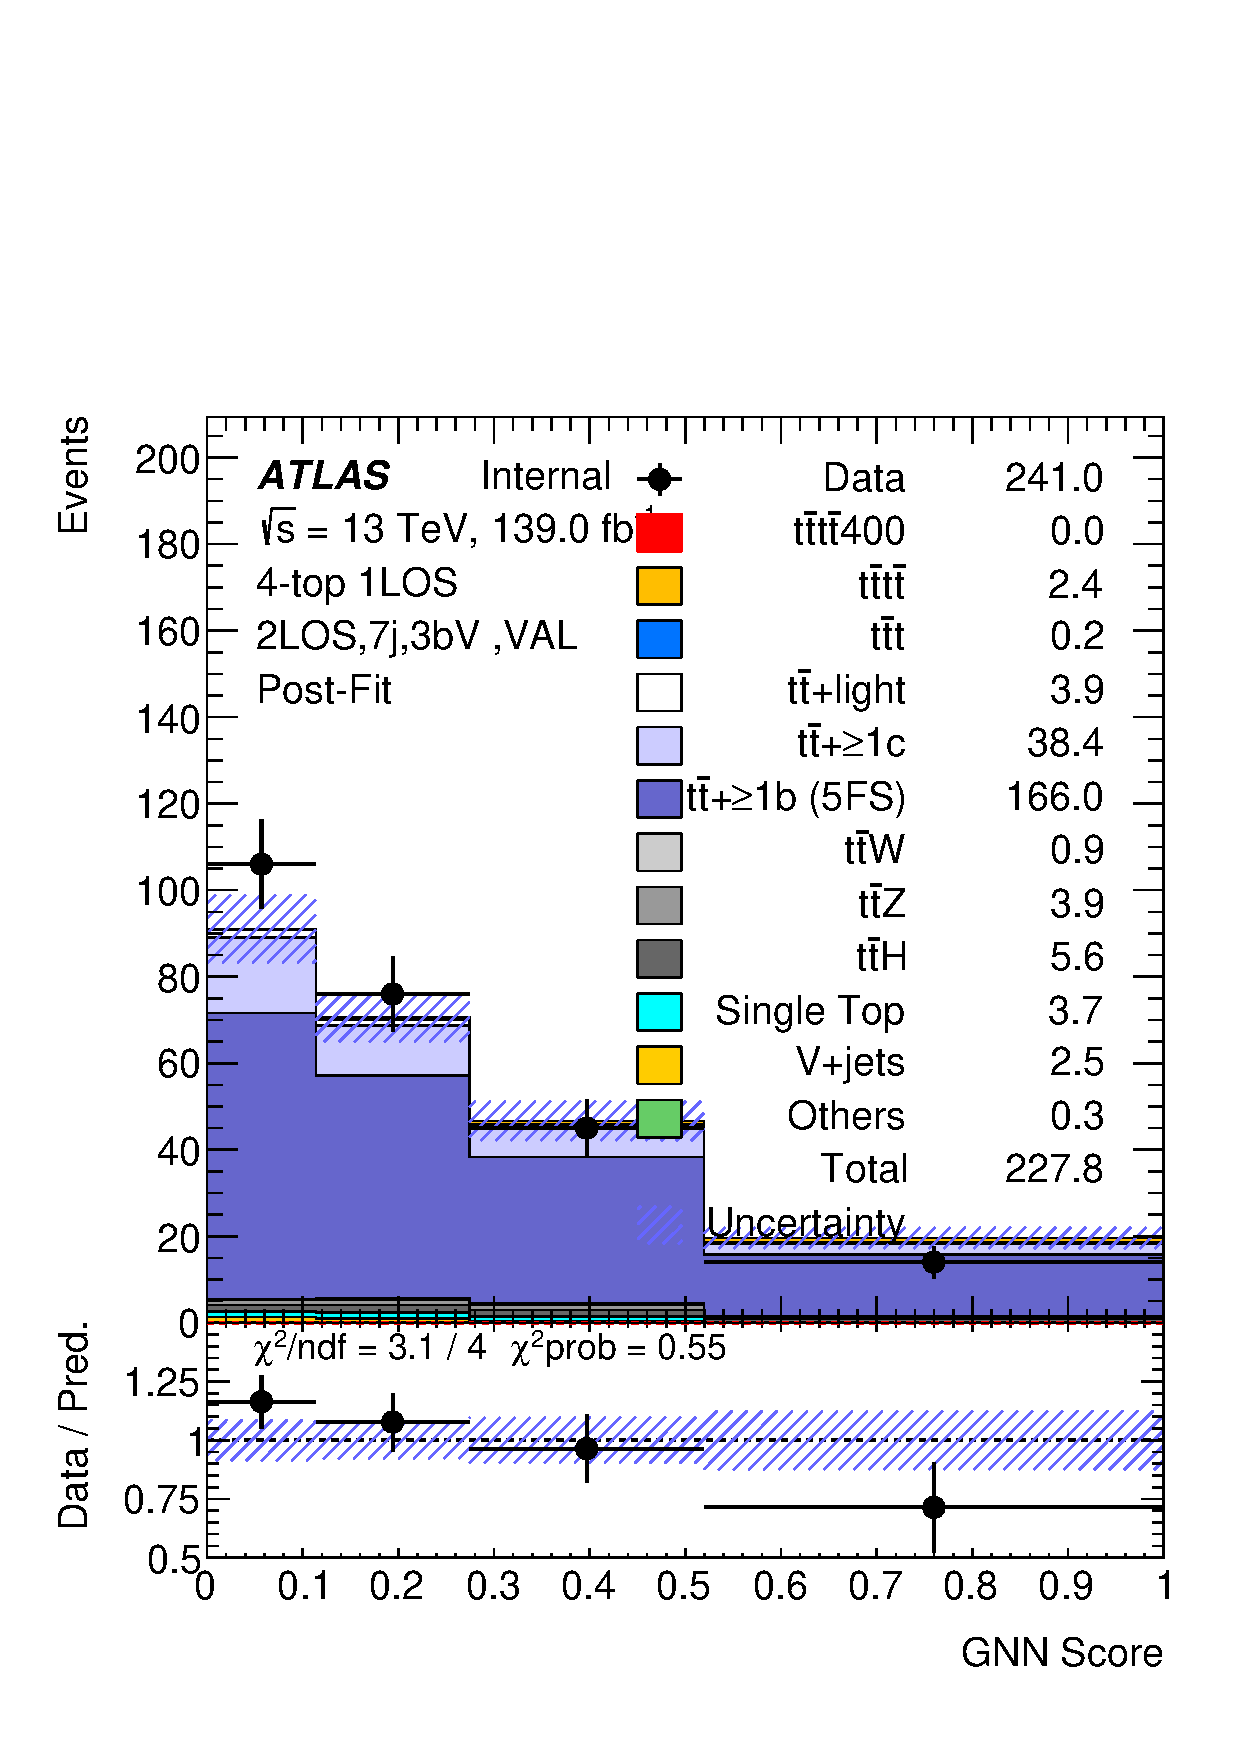
\includegraphics[width=0.23 \textwidth]{figures/fits/GNN/400/all/data_unblindedBonly/Plots/val_os2l_7j3bV_MVA_postFit.pdf} \\

        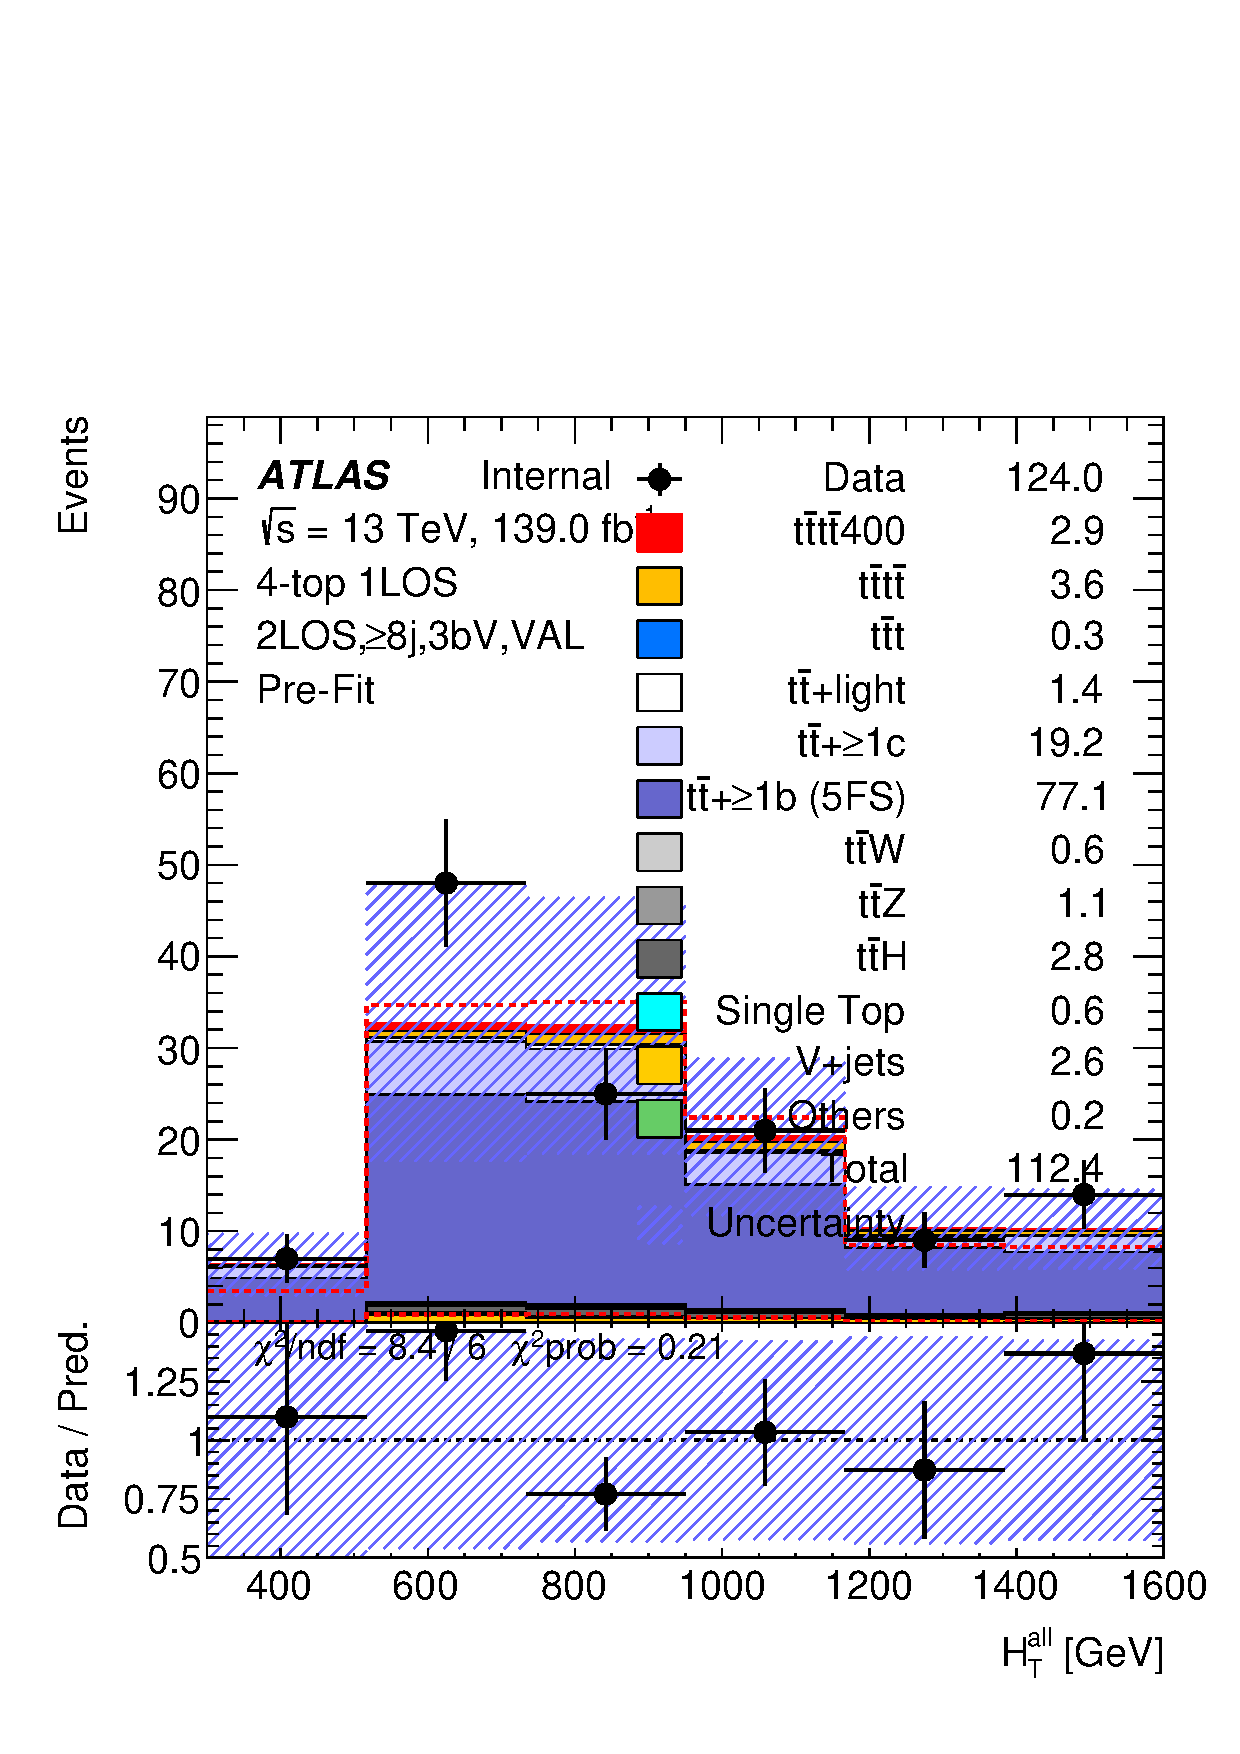
\includegraphics[width=0.23 \textwidth]{figures/fits/GNN/400/all/data_unblindedBonly/Plots/val_os2l_ge8j3bV_HT_all.pdf} &
        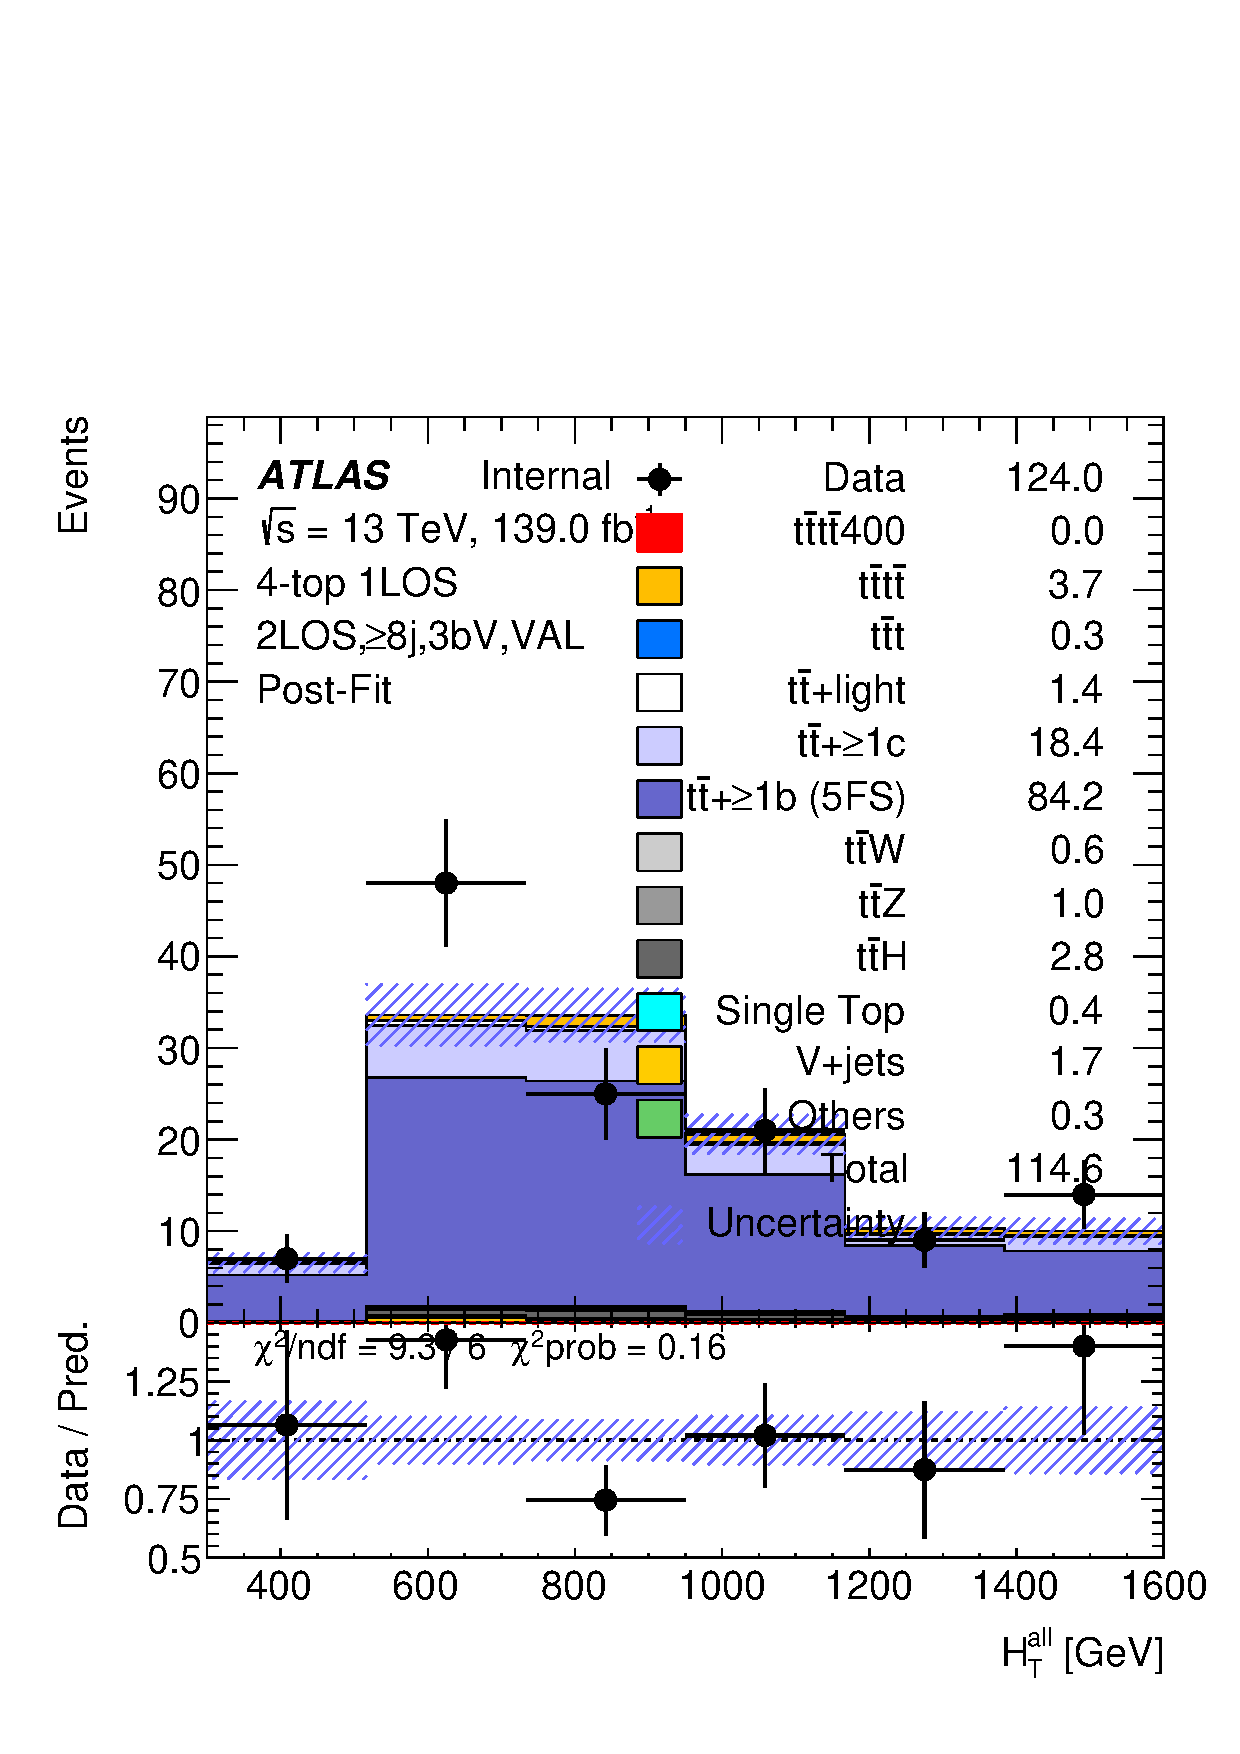
\includegraphics[width=0.23 \textwidth]{figures/fits/GNN/400/all/data_unblindedBonly/Plots/val_os2l_ge8j3bV_HT_all_postFit.pdf} &
        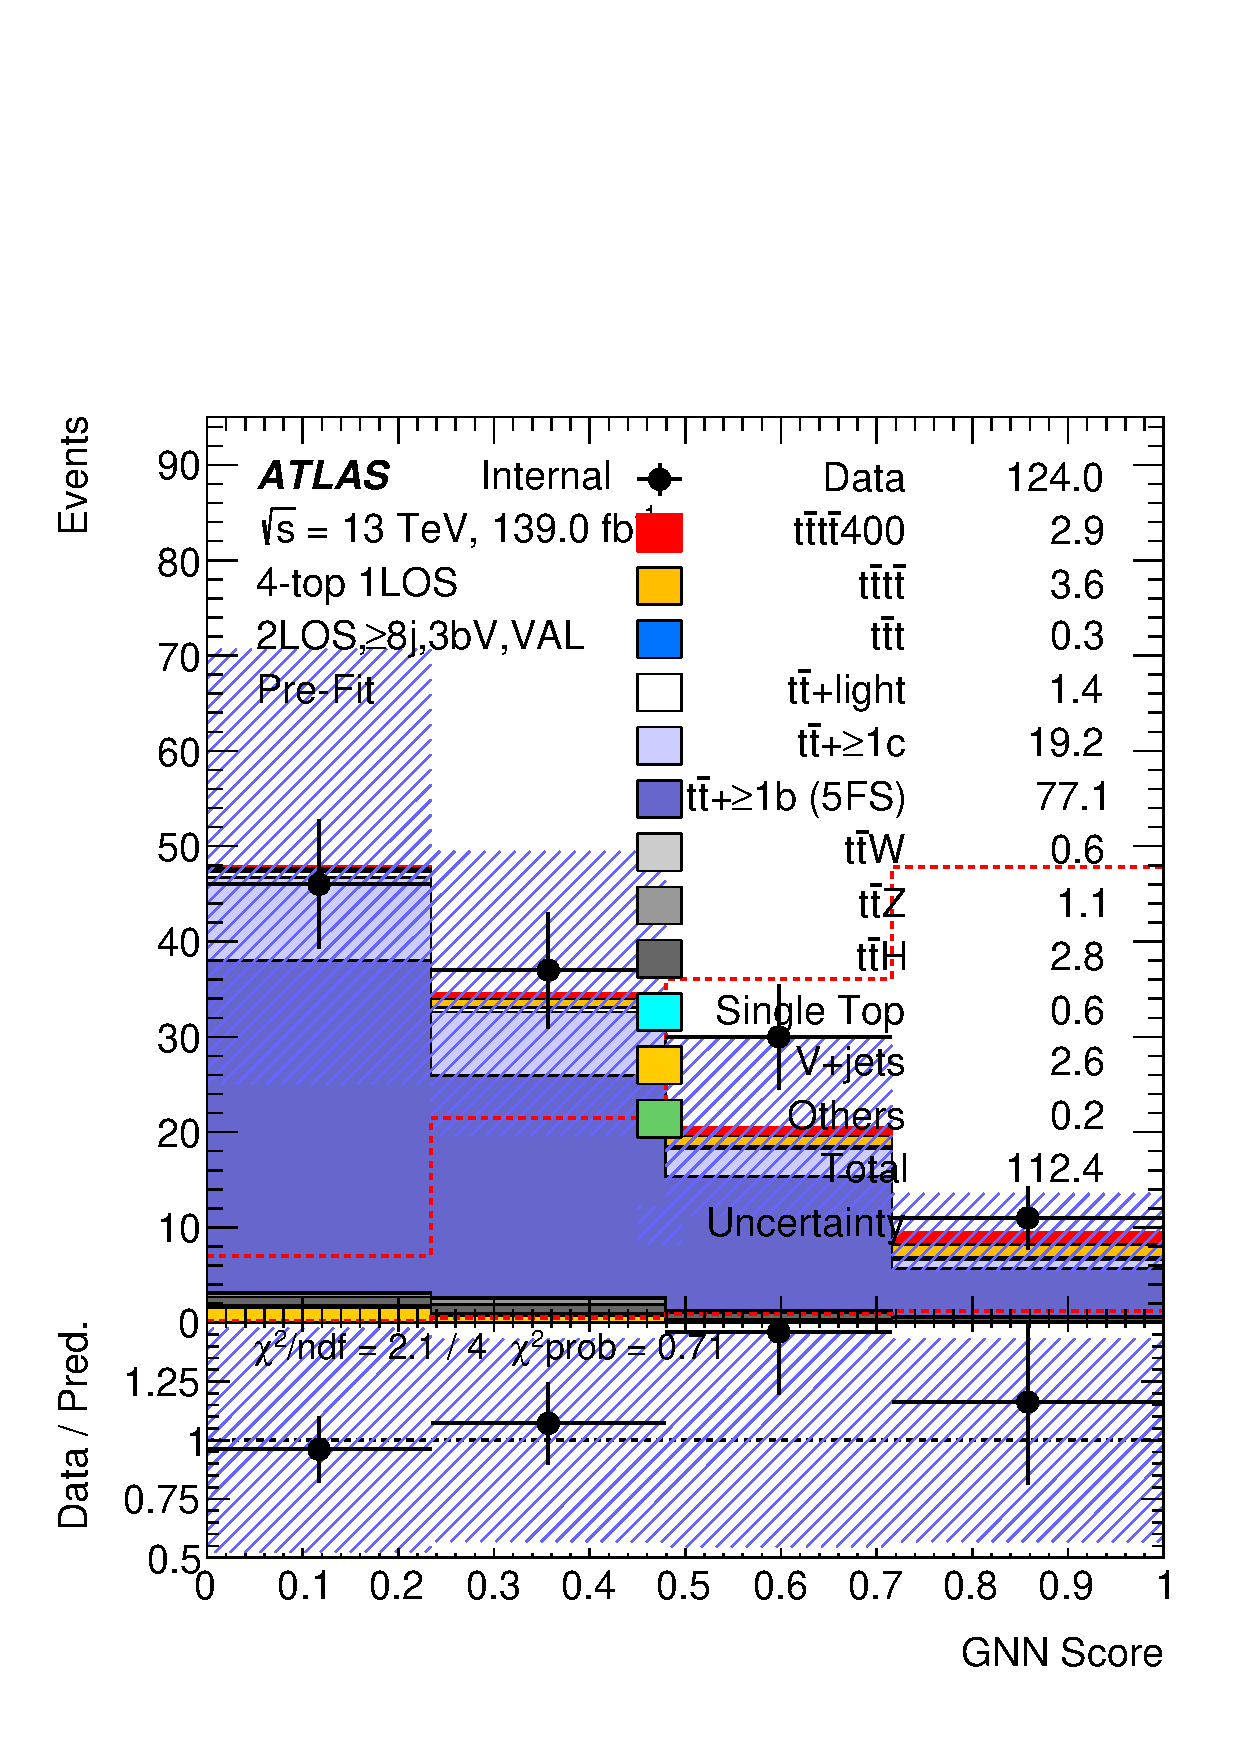
\includegraphics[width=0.23 \textwidth]{figures/fits/GNN/400/all/data_unblindedBonly/Plots/val_os2l_ge8j3bV_MVA.pdf} &
        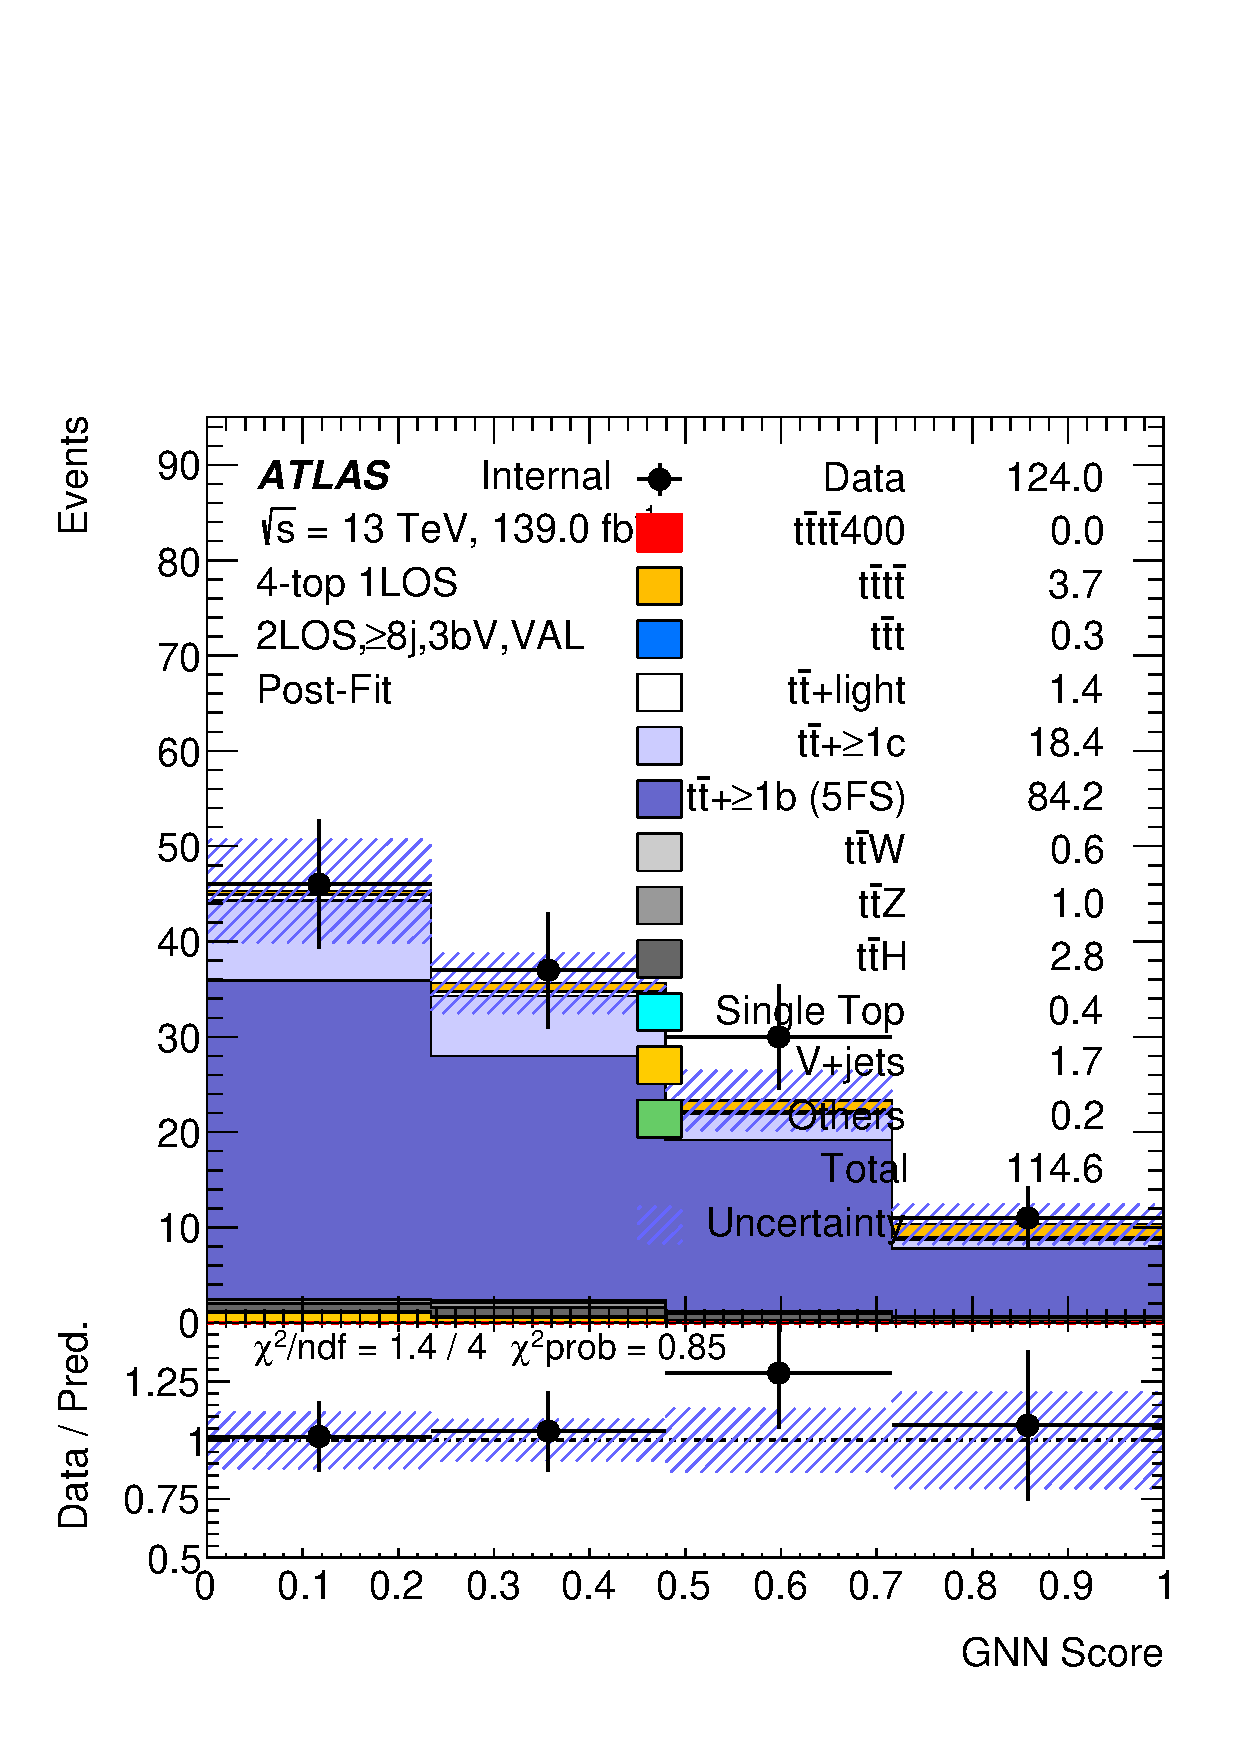
\includegraphics[width=0.23 \textwidth]{figures/fits/GNN/400/all/data_unblindedBonly/Plots/val_os2l_ge8j3bV_MVA_postFit.pdf} \\
        \end{tabular}
        \end{center}
        \caption{\label{val_region_fig2}Pre-fit and Post-fit distribution in 3bV 2L validation regions. First row shows os2l(7j3bV) region and second row shows os2l(ge8j3bV) region.}
        \end{subfigure}
        \caption{\label{validation_plots}Pre-fit(Left) and Post-fit(right) distribution is shown for combined fit (1LOS).}
\end{figure}

\clearpage



\subsection{GNN Input Variable Distributions for region 1L, $\geq10$ jets, 4b}
\label{app:validation_GNN_input_1L_ge10j4b}

The pre-fit and post-fit plots for the GNN input variables are shown in Figures \ref{GNN_input_val_1}, \ref{GNN_input_val_2}, and \ref{GNN_input_val_3} from the background-only unblinded-data fits. The distributions are shown for the 1L ge10j4b region, which is one of the regions most sensitive to signal. Good MC/data agreement can be seen.

\begin{figure}
        \begin{center} \setlength{\tabcolsep}{2.5pt}\footnotesize
        \begin{tabular}{cccc}
        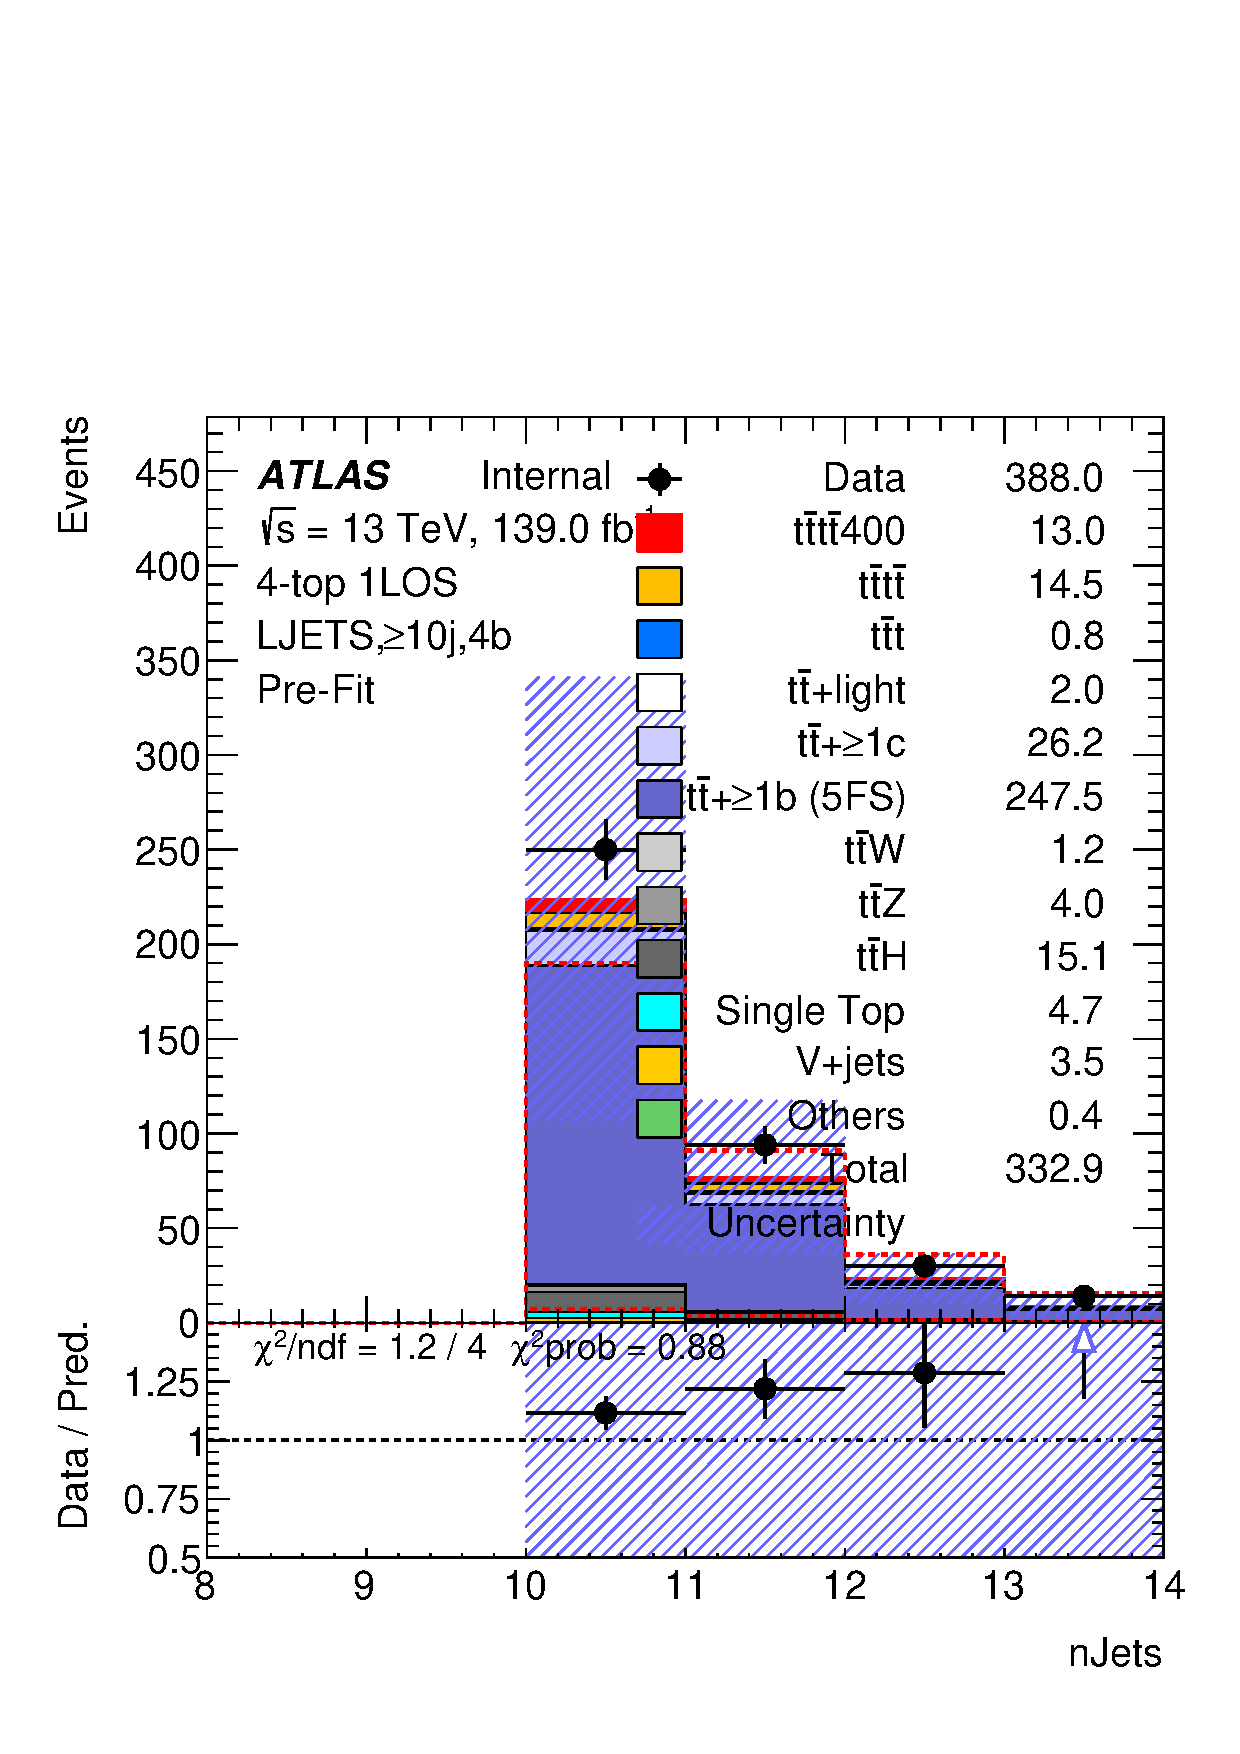
\includegraphics[width=0.23 \textwidth]{figures/fits/GNN/400/all/data_unblindedBonly/Plots/val_ljets_ge10j4b_nJets.pdf} &
        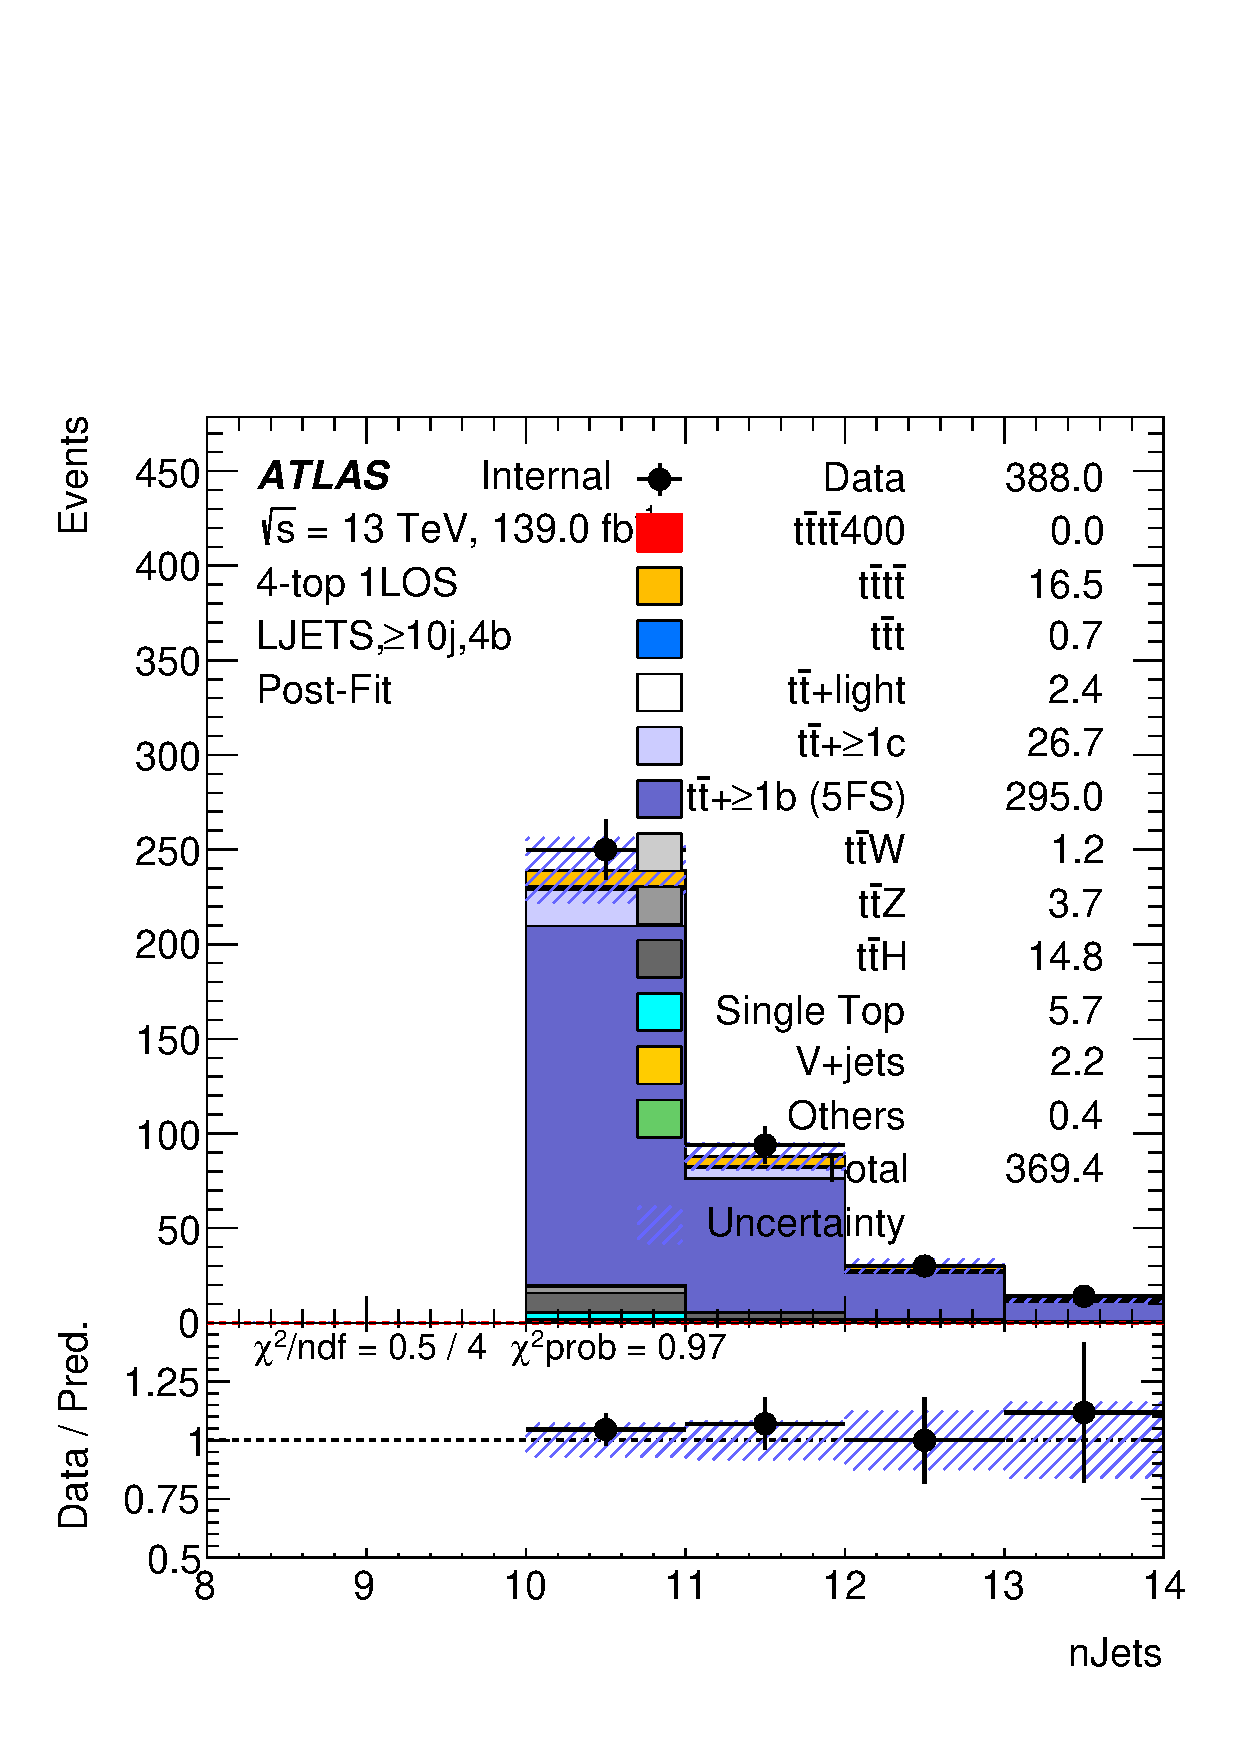
\includegraphics[width=0.23 \textwidth]{figures/fits/GNN/400/all/data_unblindedBonly/Plots/val_ljets_ge10j4b_nJets_postFit.pdf} &
        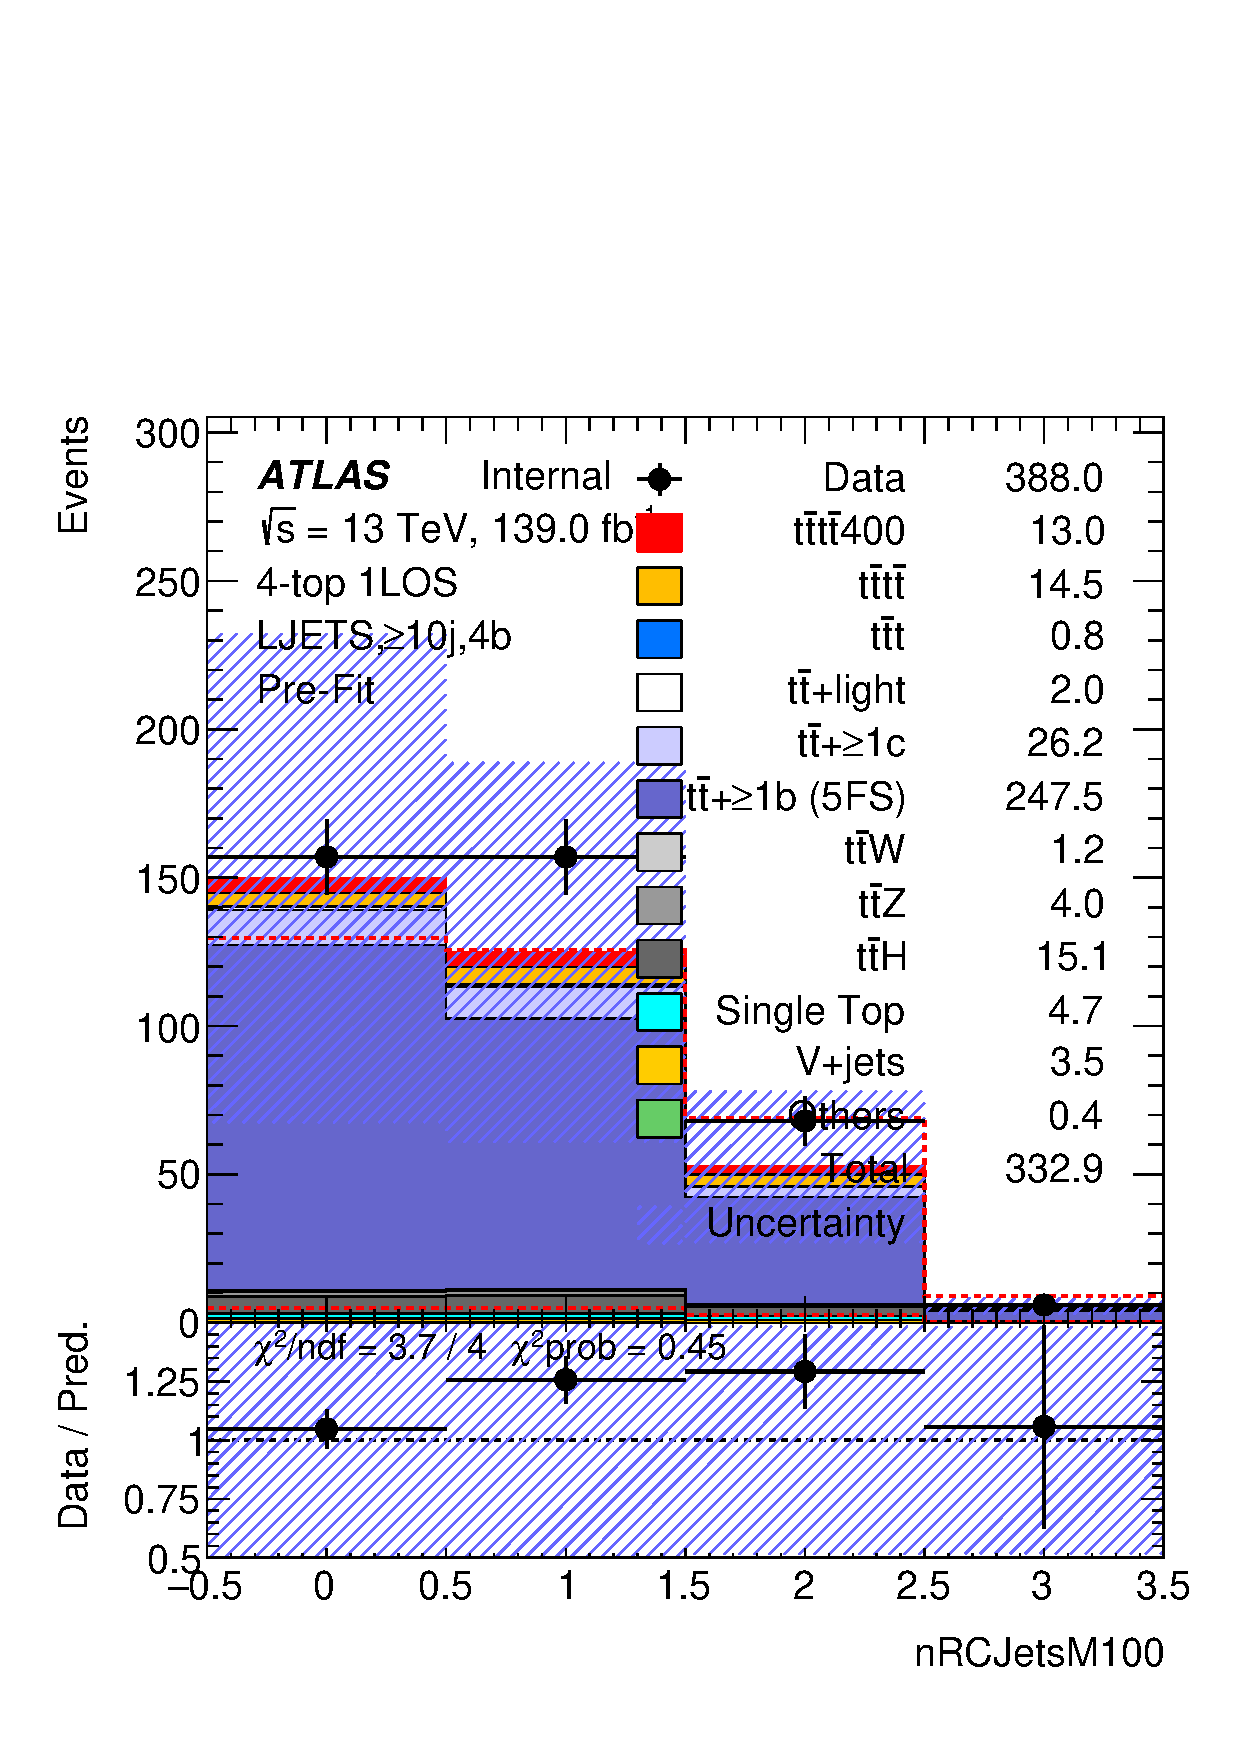
\includegraphics[width=0.23 \textwidth]{figures/fits/GNN/400/all/data_unblindedBonly/Plots/val_ljets_ge10j4b_nRCJetsM100.pdf} &
        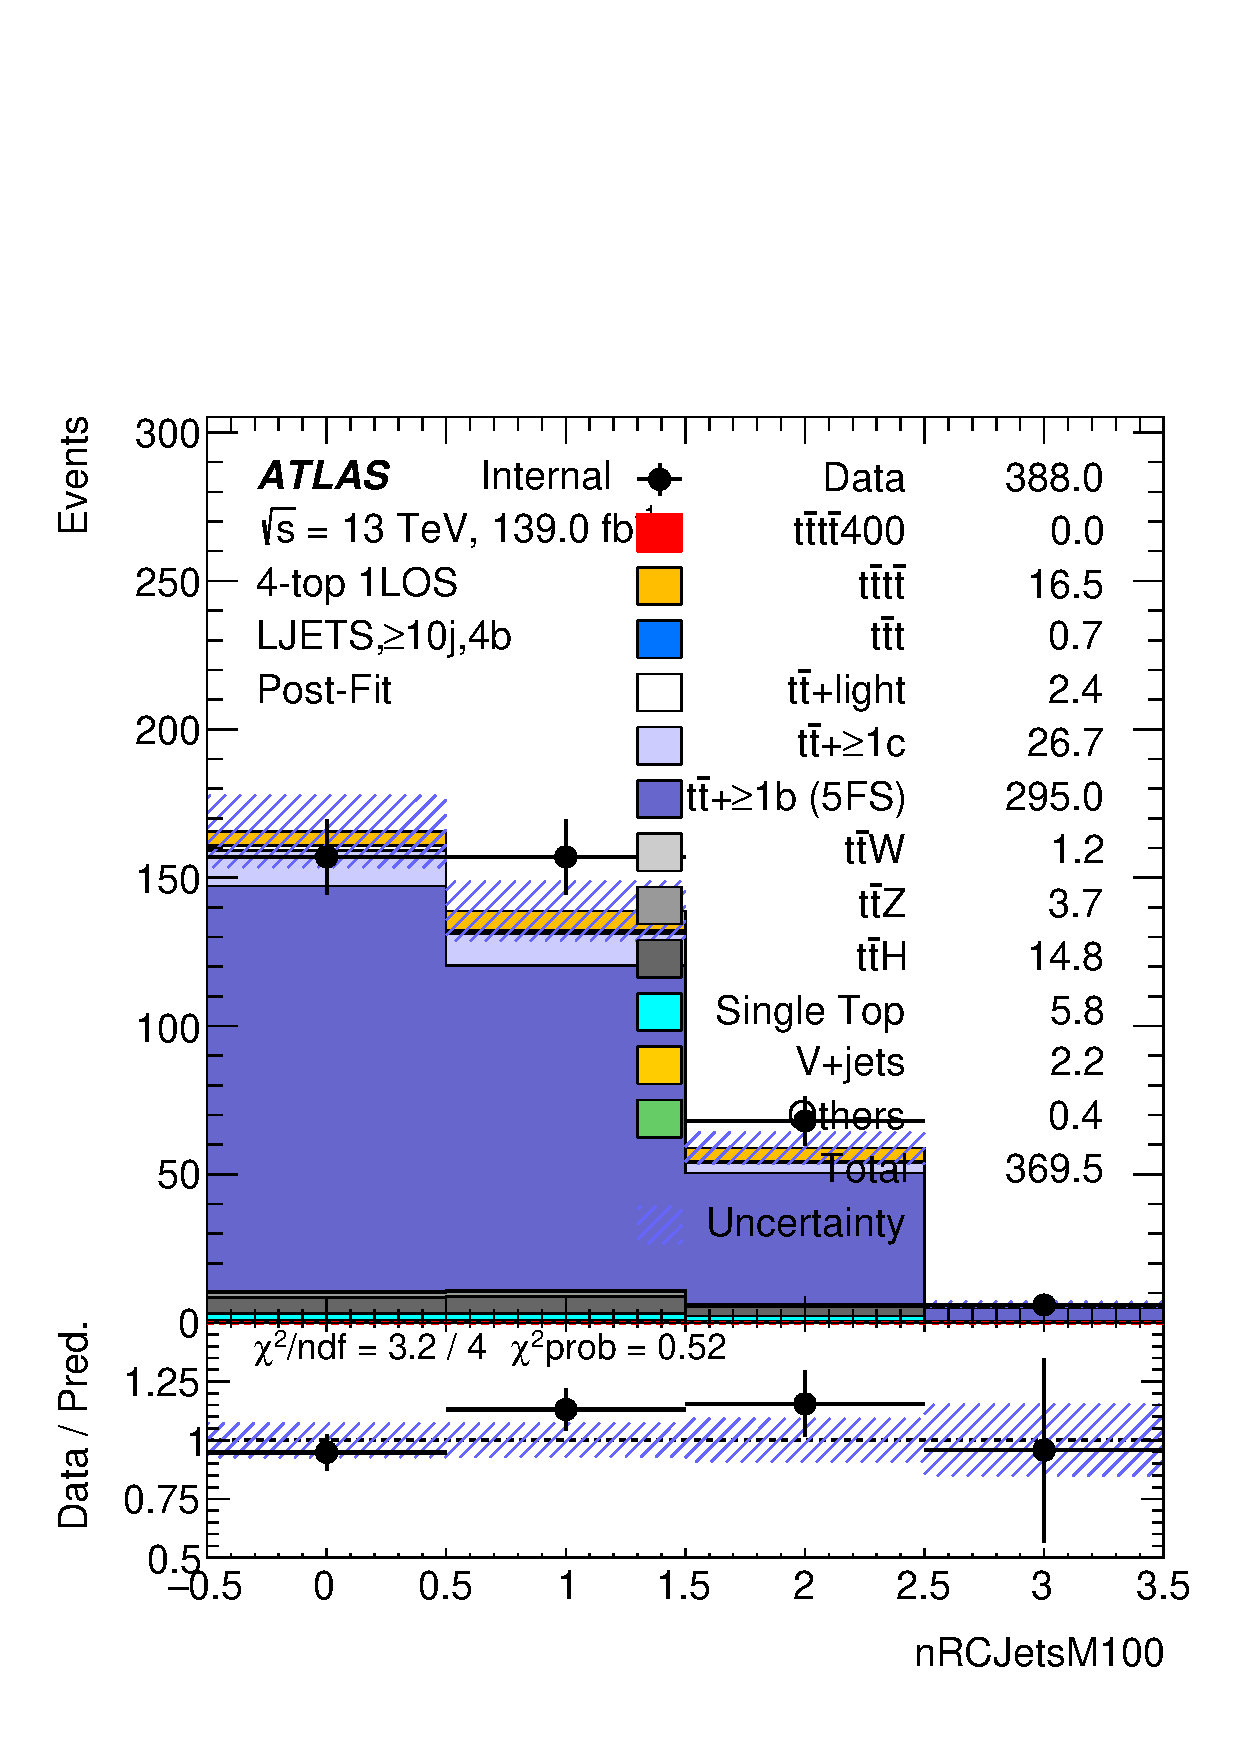
\includegraphics[width=0.23 \textwidth]{figures/fits/GNN/400/all/data_unblindedBonly/Plots/val_ljets_ge10j4b_nRCJetsM100_postFit.pdf} \\

        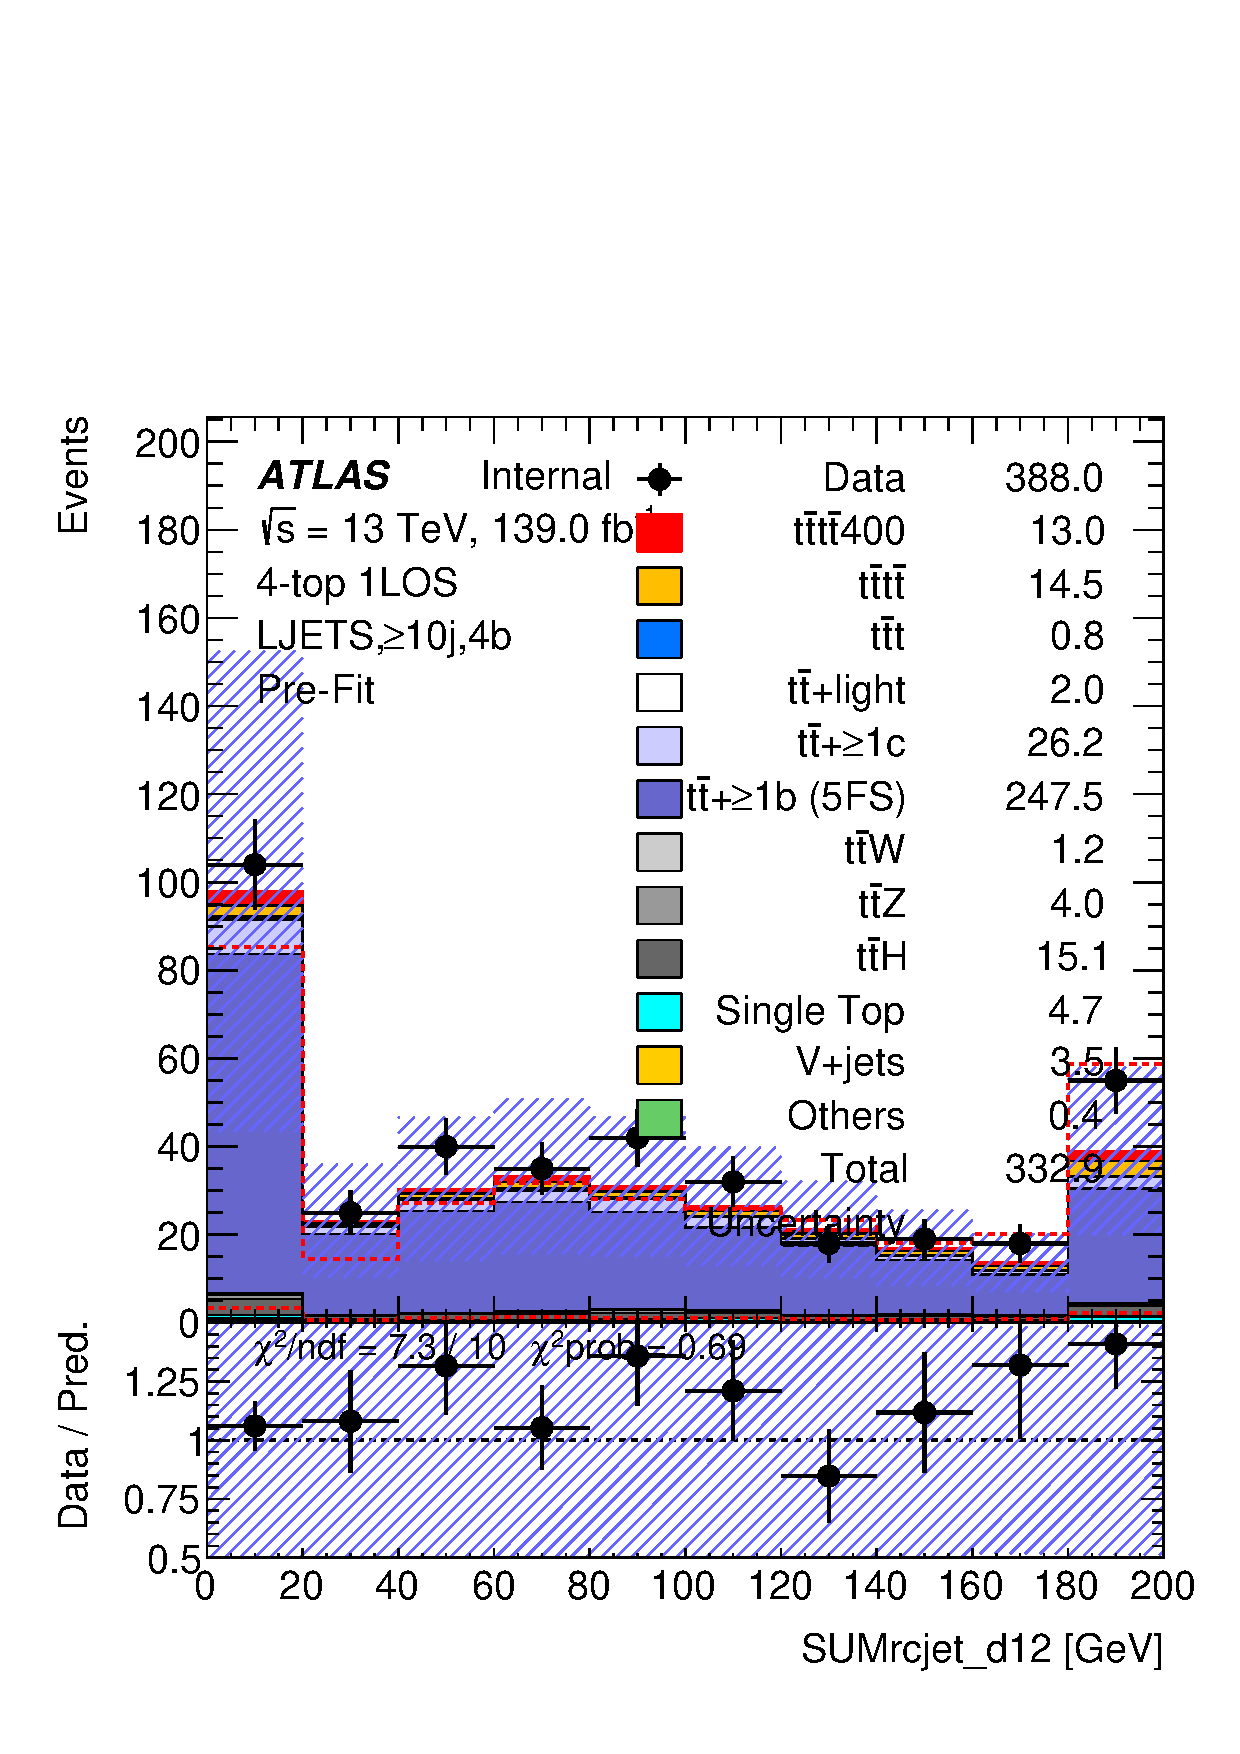
\includegraphics[width=0.23 \textwidth]{figures/fits/GNN/400/all/data_unblindedBonly/Plots/val_ljets_ge10j4b_sum_rcjet_d12.pdf} &
        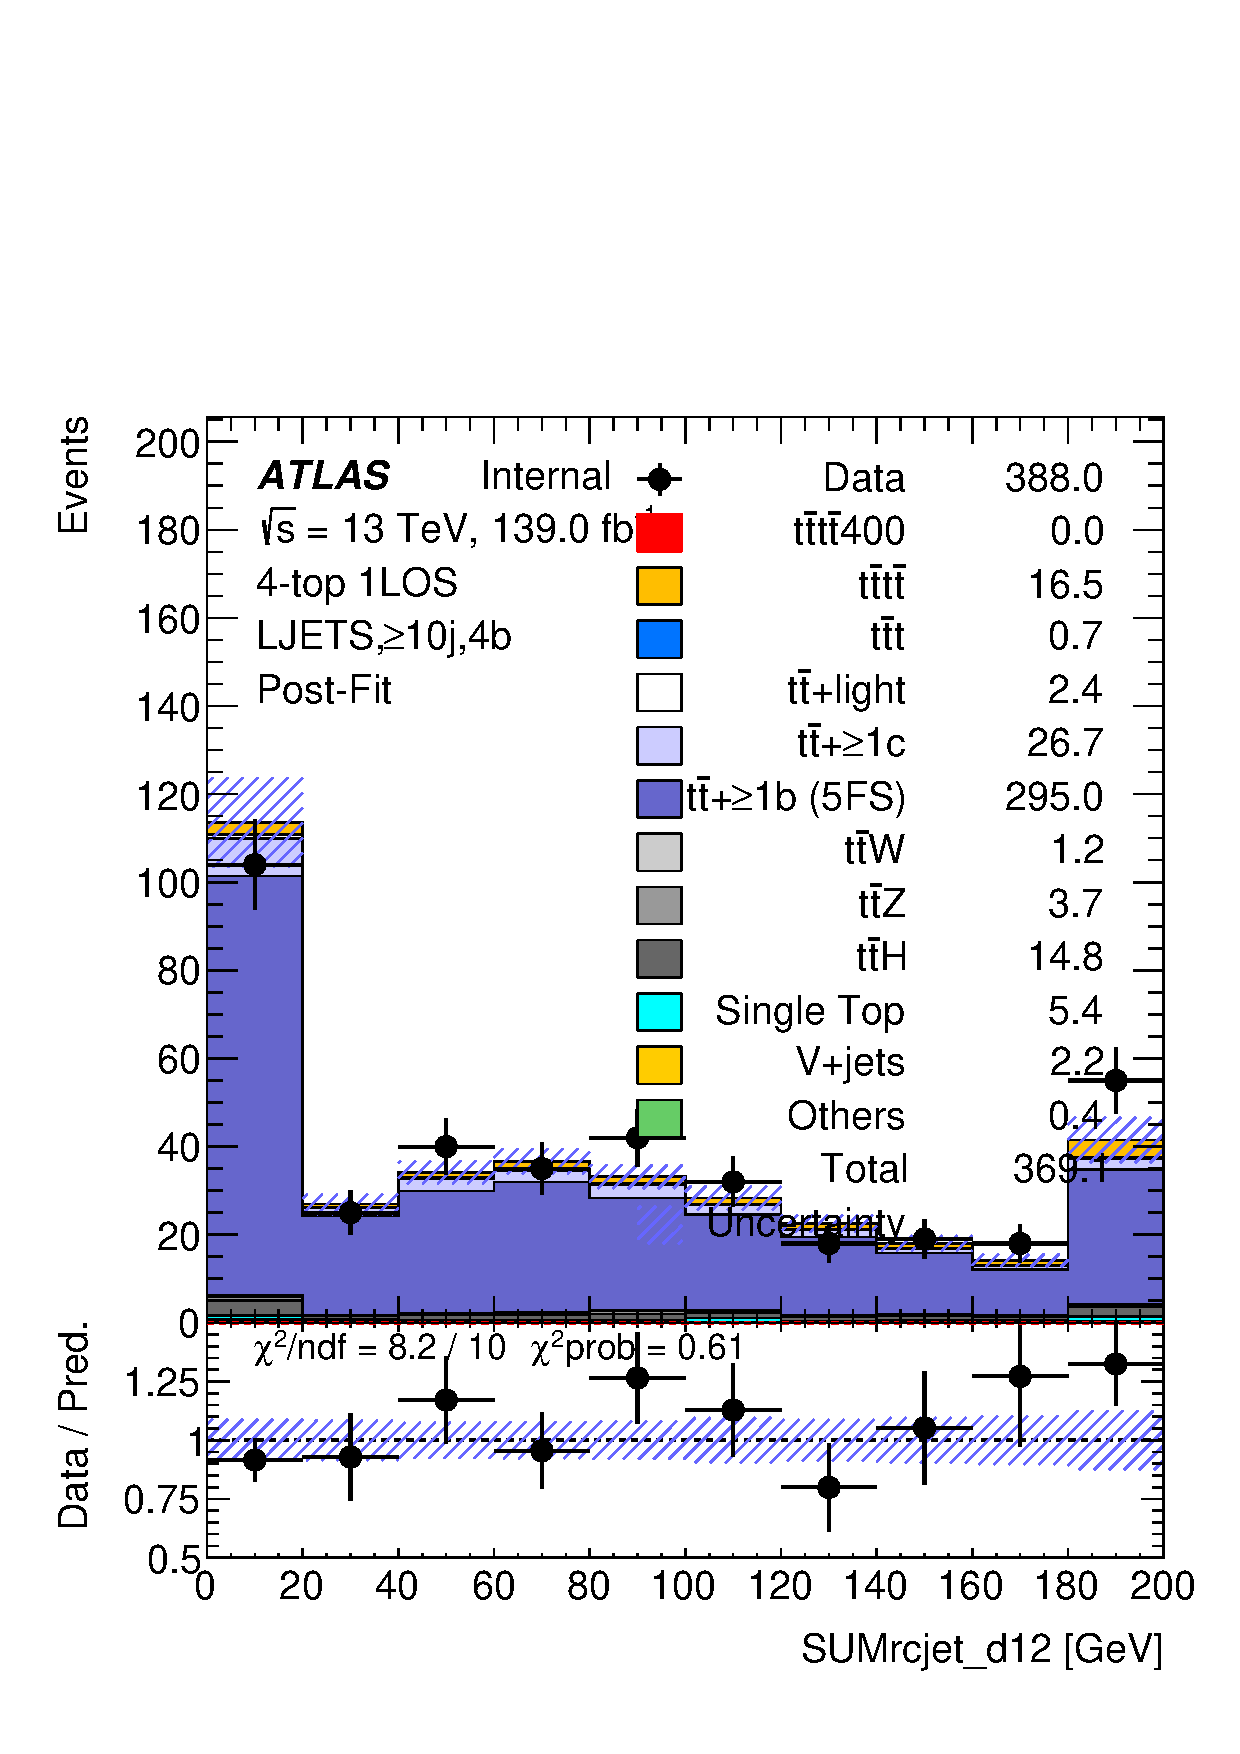
\includegraphics[width=0.23 \textwidth]{figures/fits/GNN/400/all/data_unblindedBonly/Plots/val_ljets_ge10j4b_sum_rcjet_d12_postFit.pdf} &
        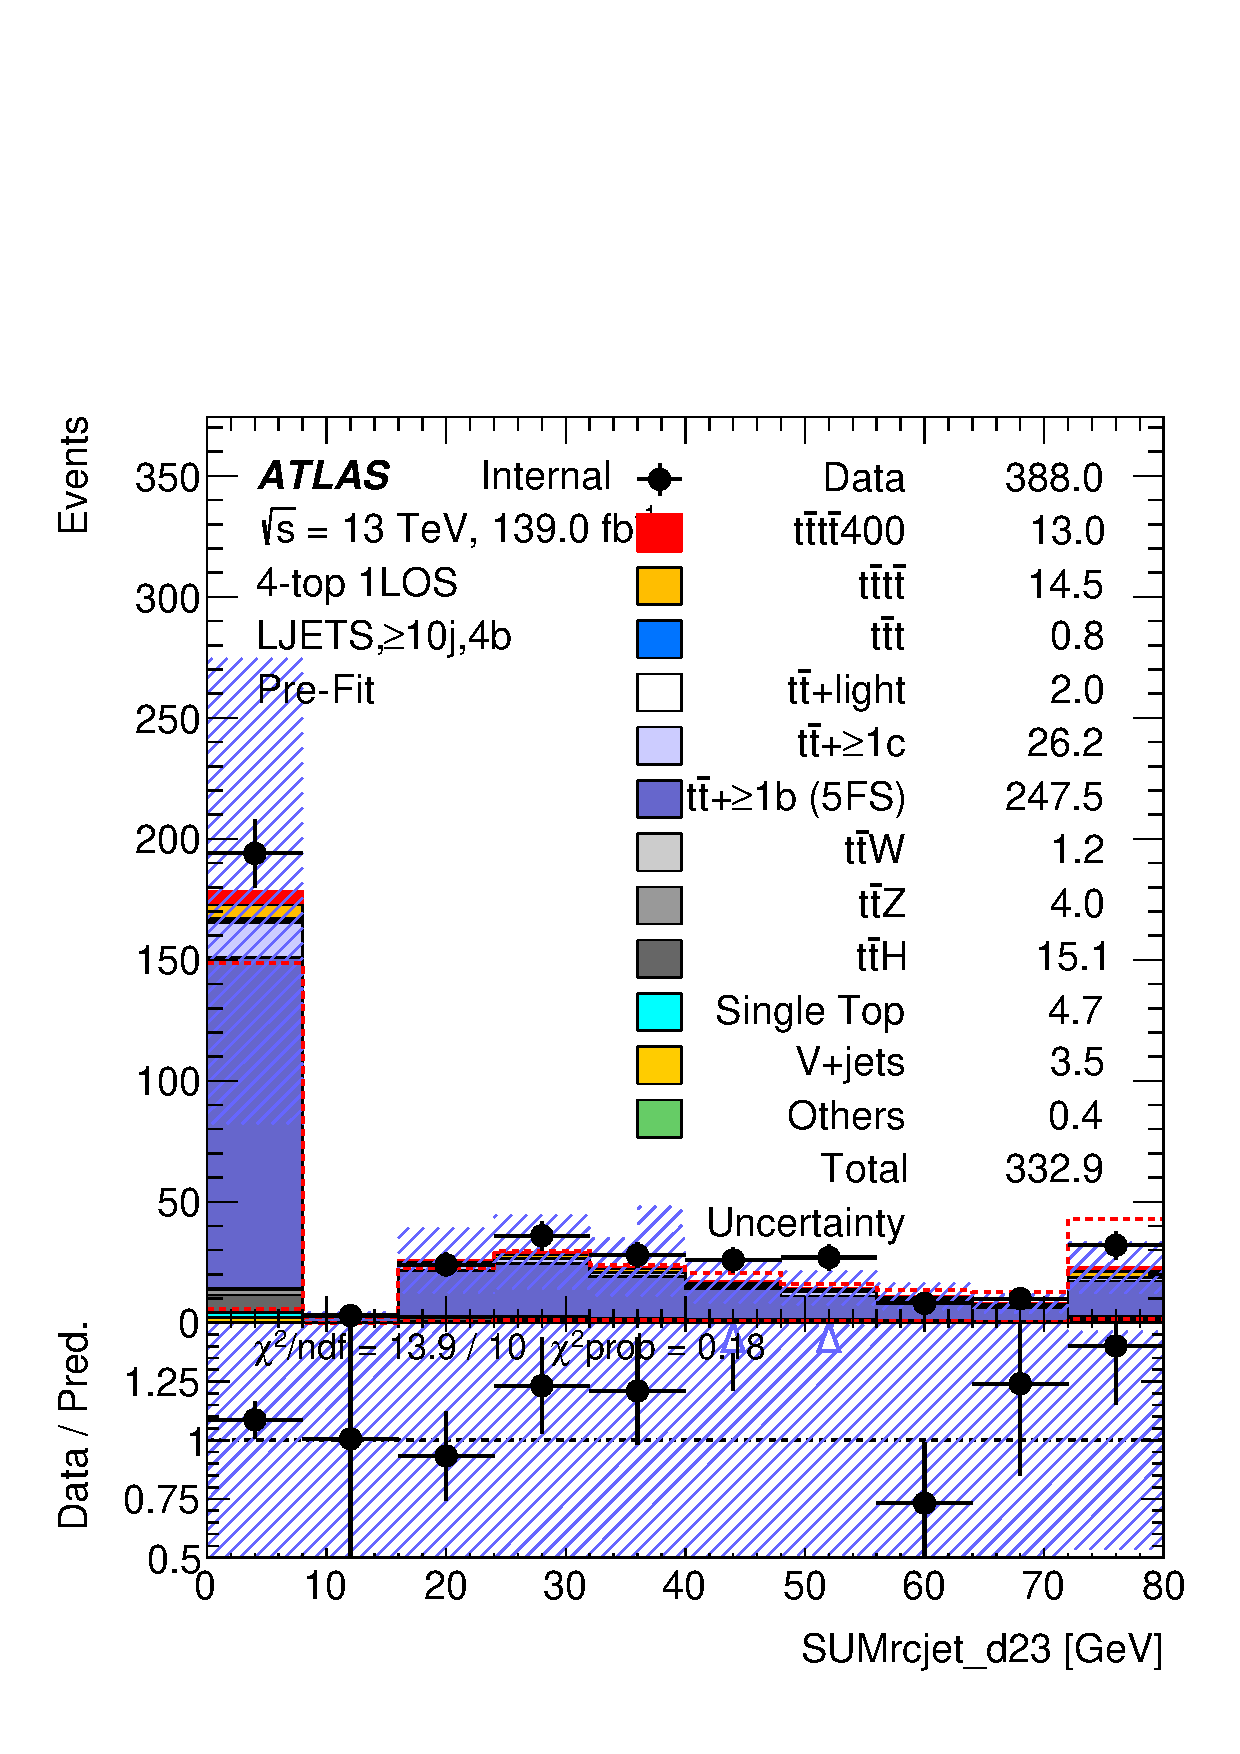
\includegraphics[width=0.23 \textwidth]{figures/fits/GNN/400/all/data_unblindedBonly/Plots/val_ljets_ge10j4b_sum_rcjet_d23.pdf} &
        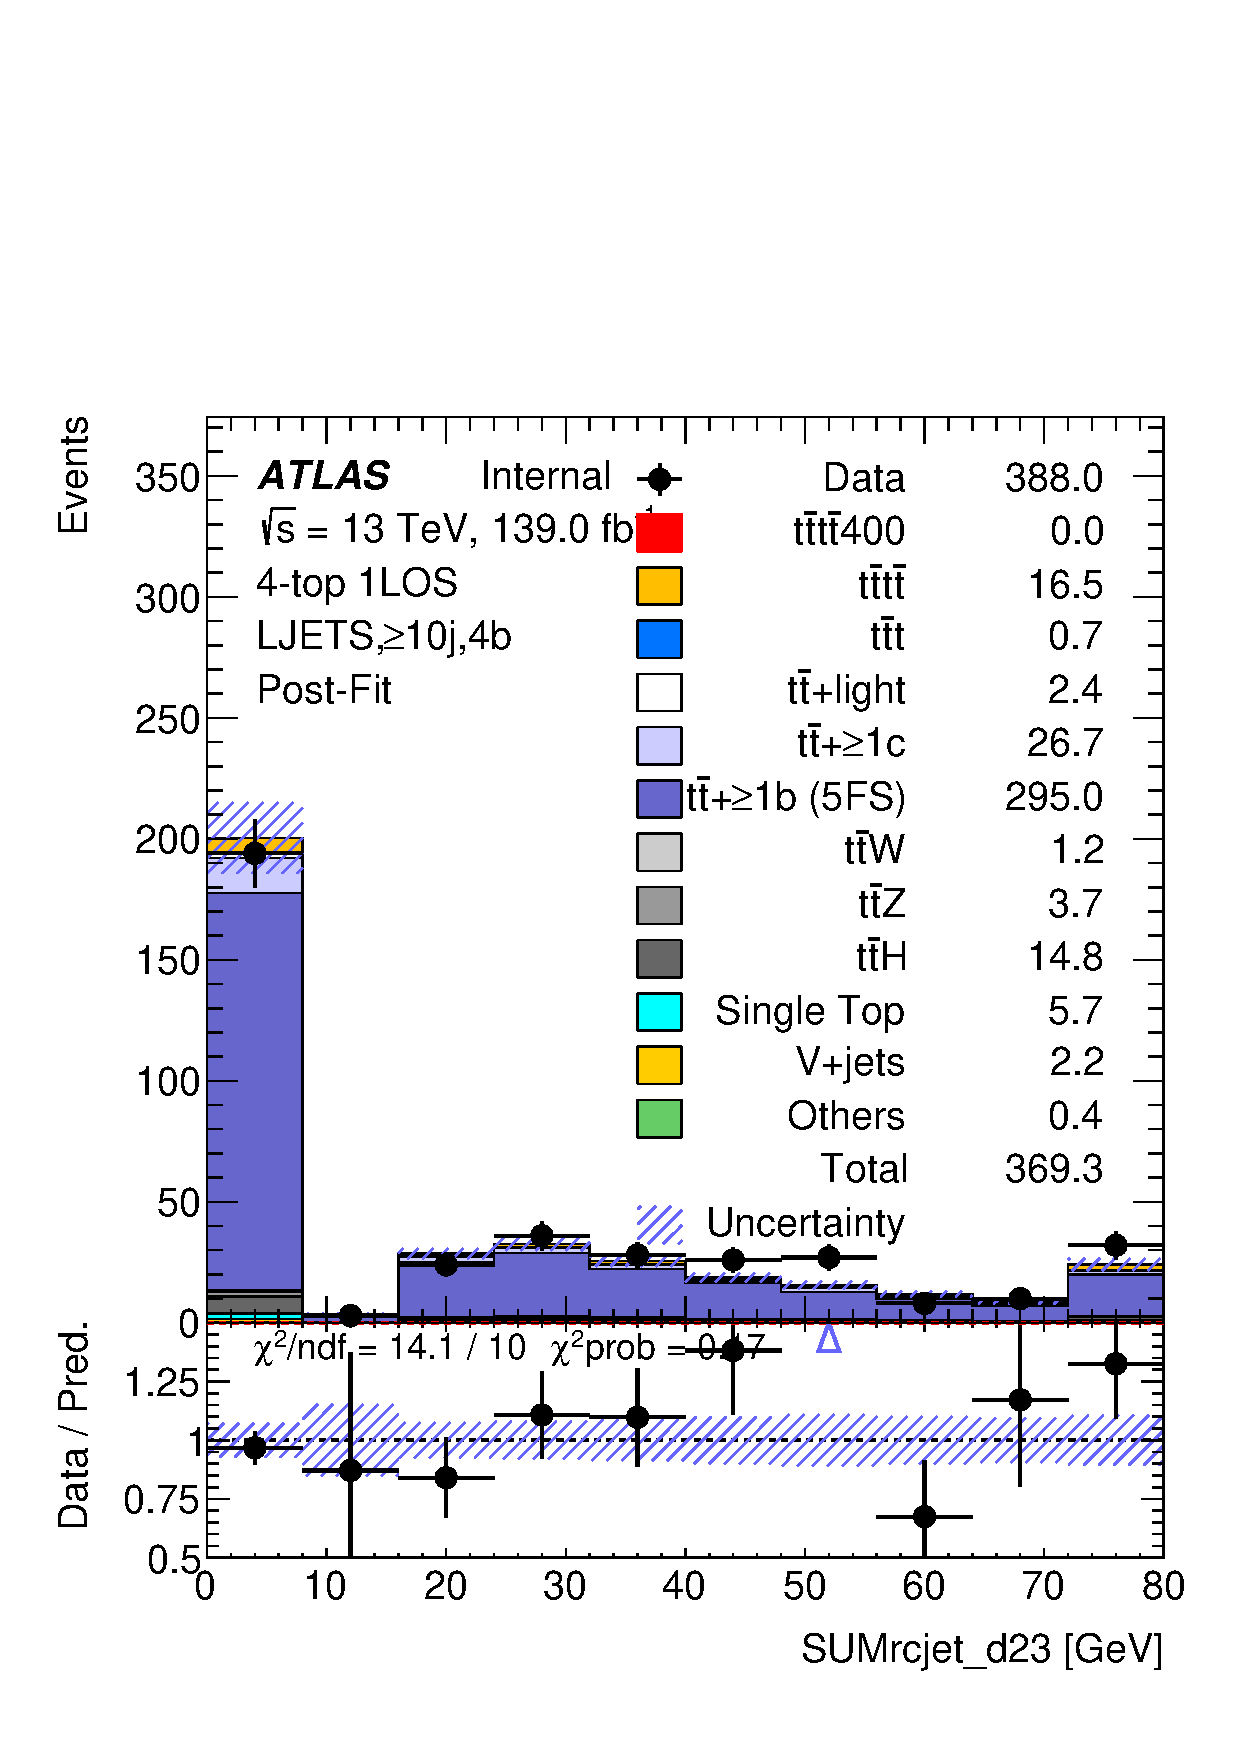
\includegraphics[width=0.23 \textwidth]{figures/fits/GNN/400/all/data_unblindedBonly/Plots/val_ljets_ge10j4b_sum_rcjet_d23_postFit.pdf} \\

        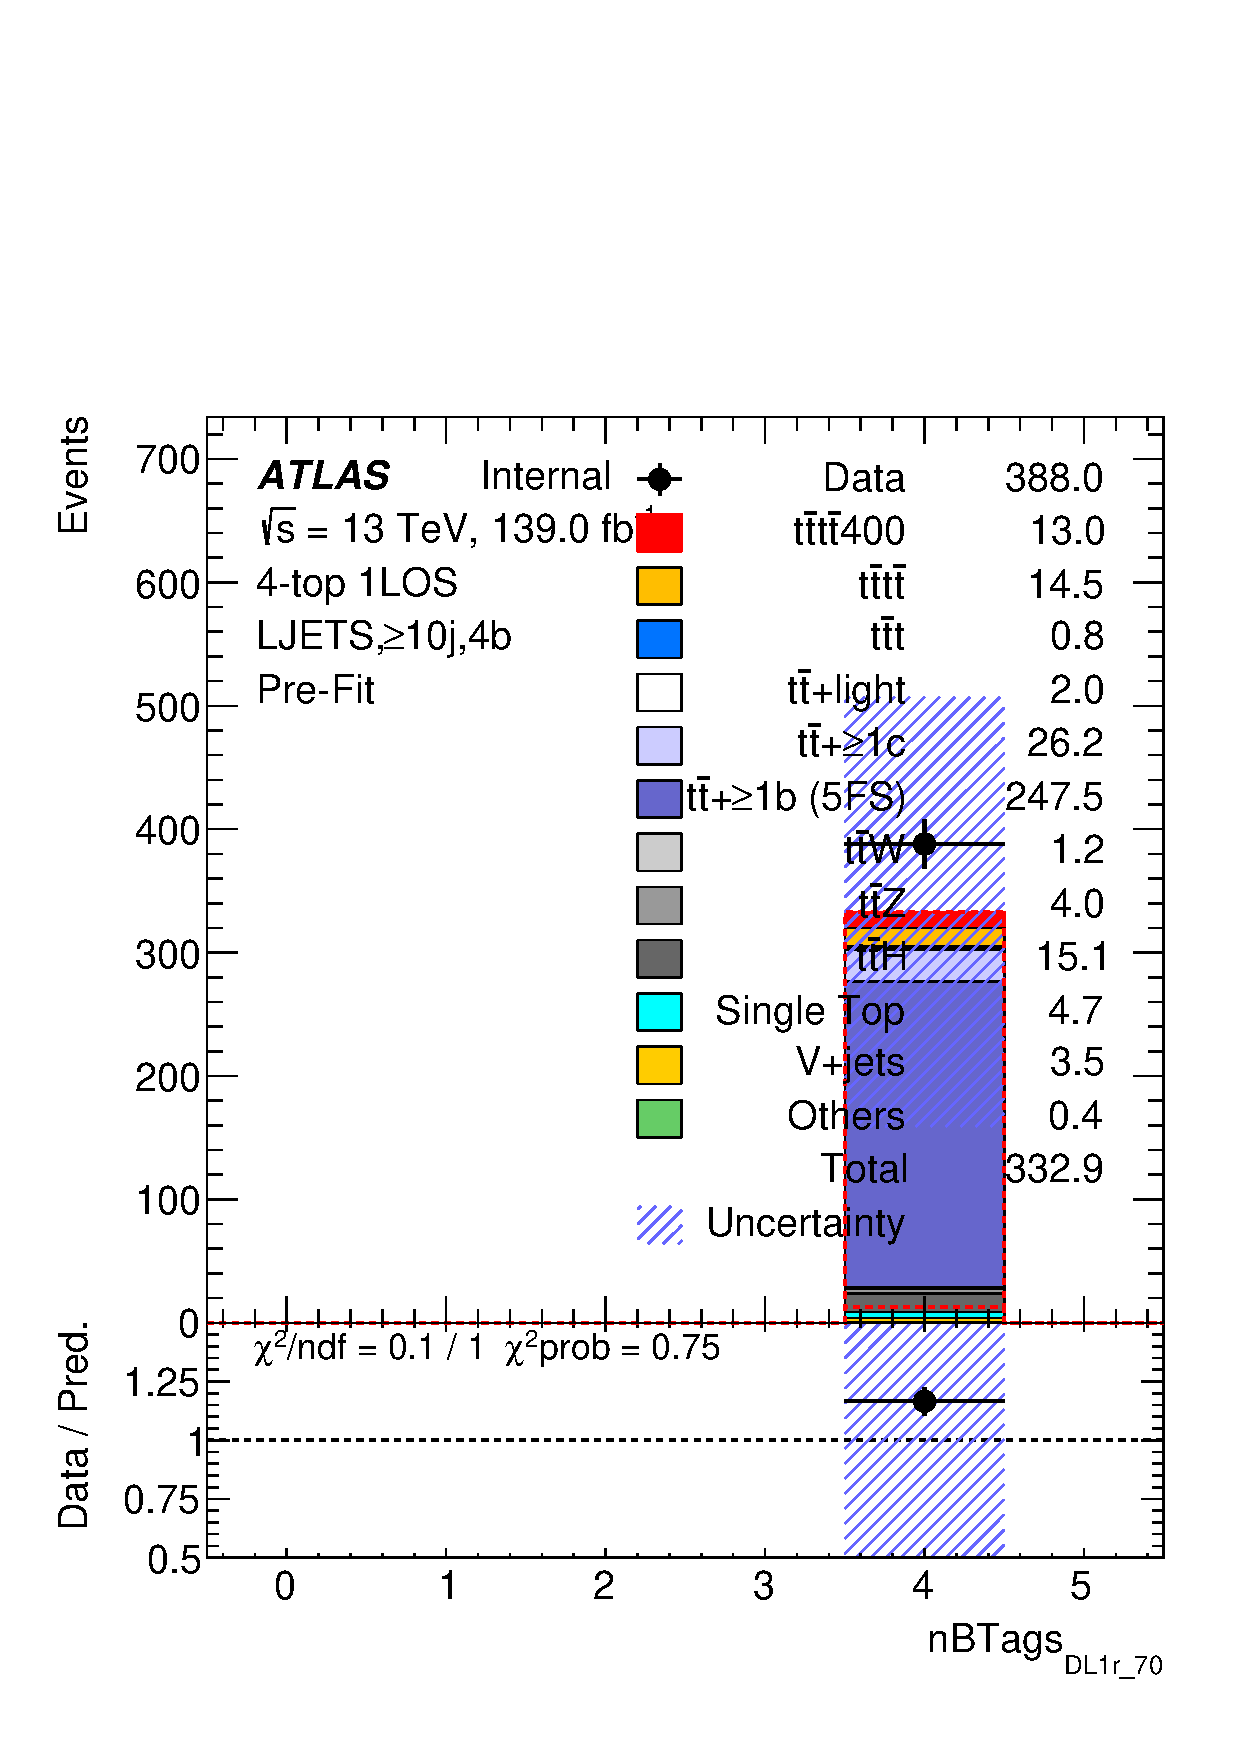
\includegraphics[width=0.23 \textwidth]{figures/fits/GNN/400/all/data_unblindedBonly/Plots/val_ljets_ge10j4b_nBTags_DL1r_70.pdf} &
        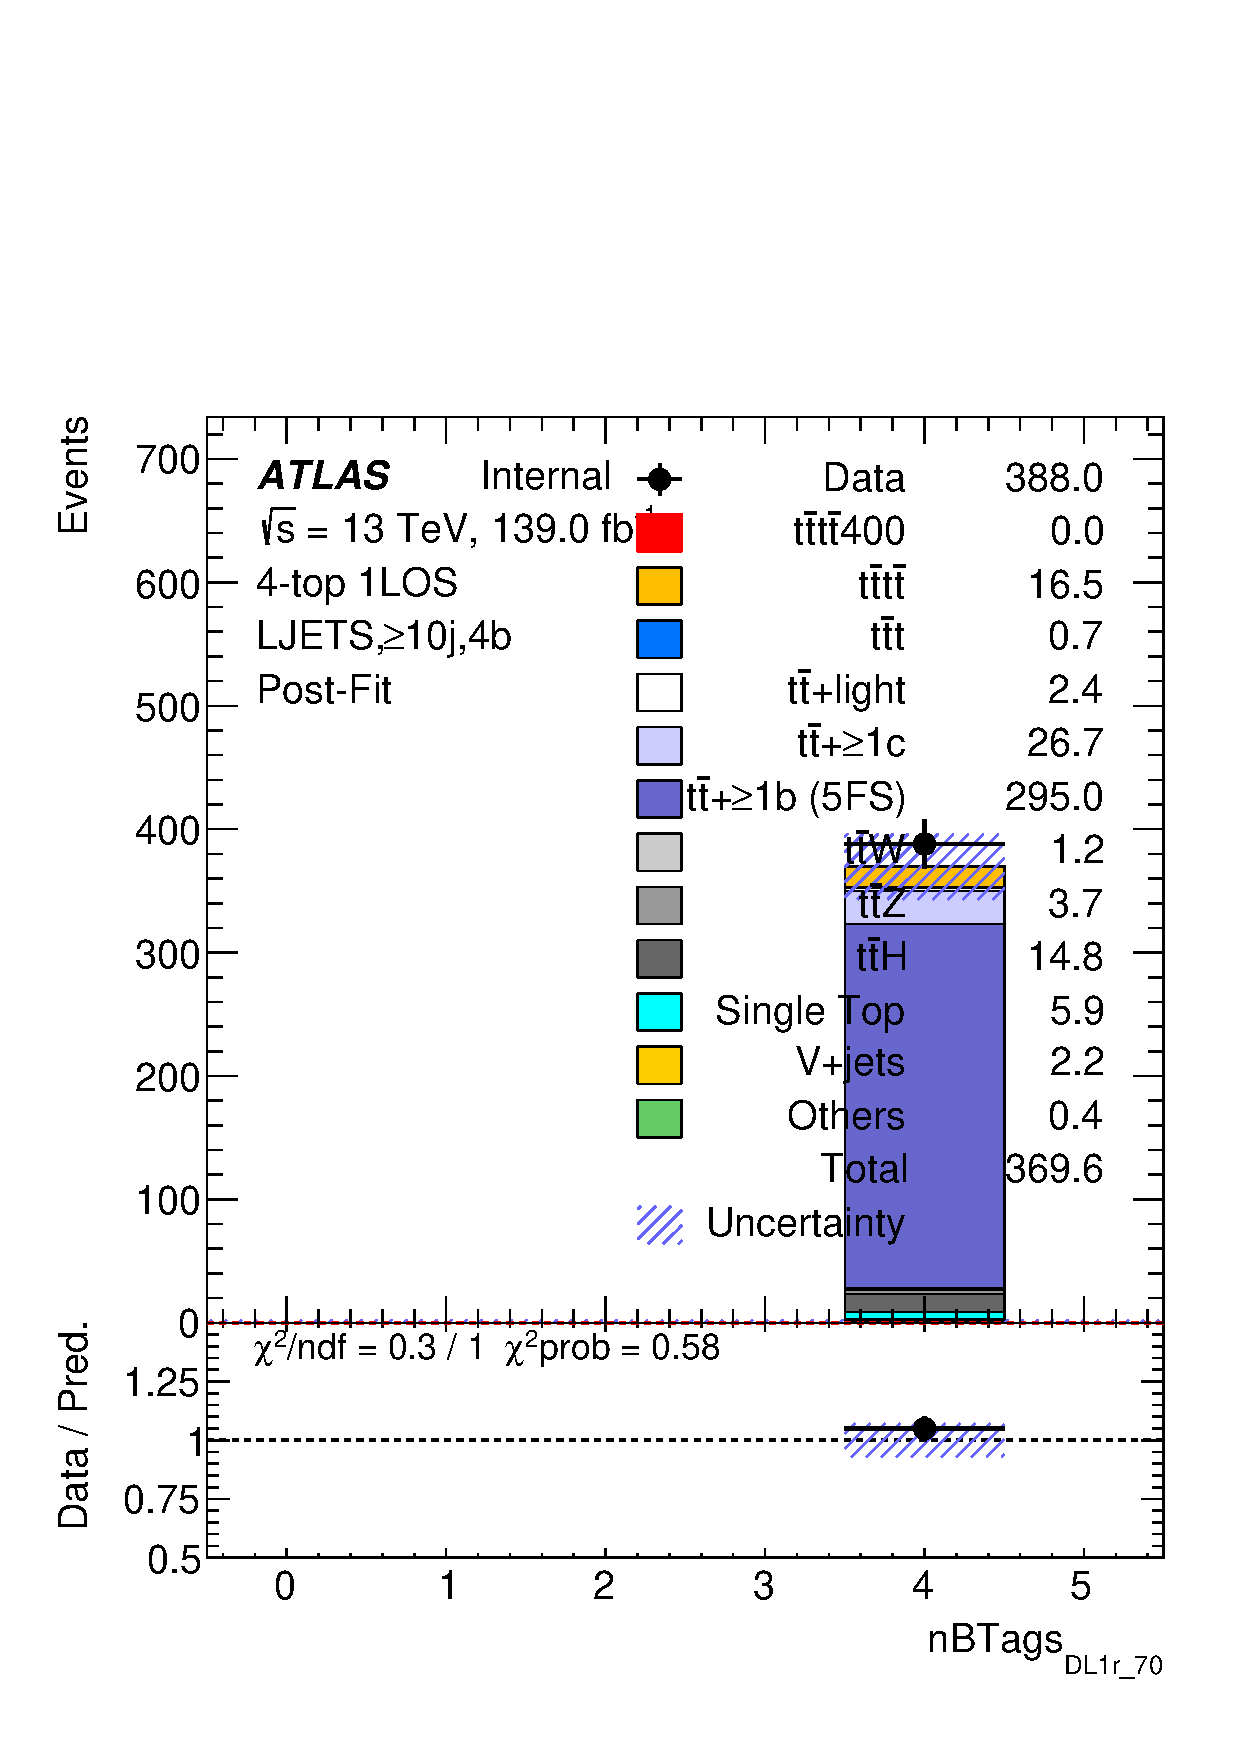
\includegraphics[width=0.23 \textwidth]{figures/fits/GNN/400/all/data_unblindedBonly/Plots/val_ljets_ge10j4b_nBTags_DL1r_70_postFit.pdf} &
        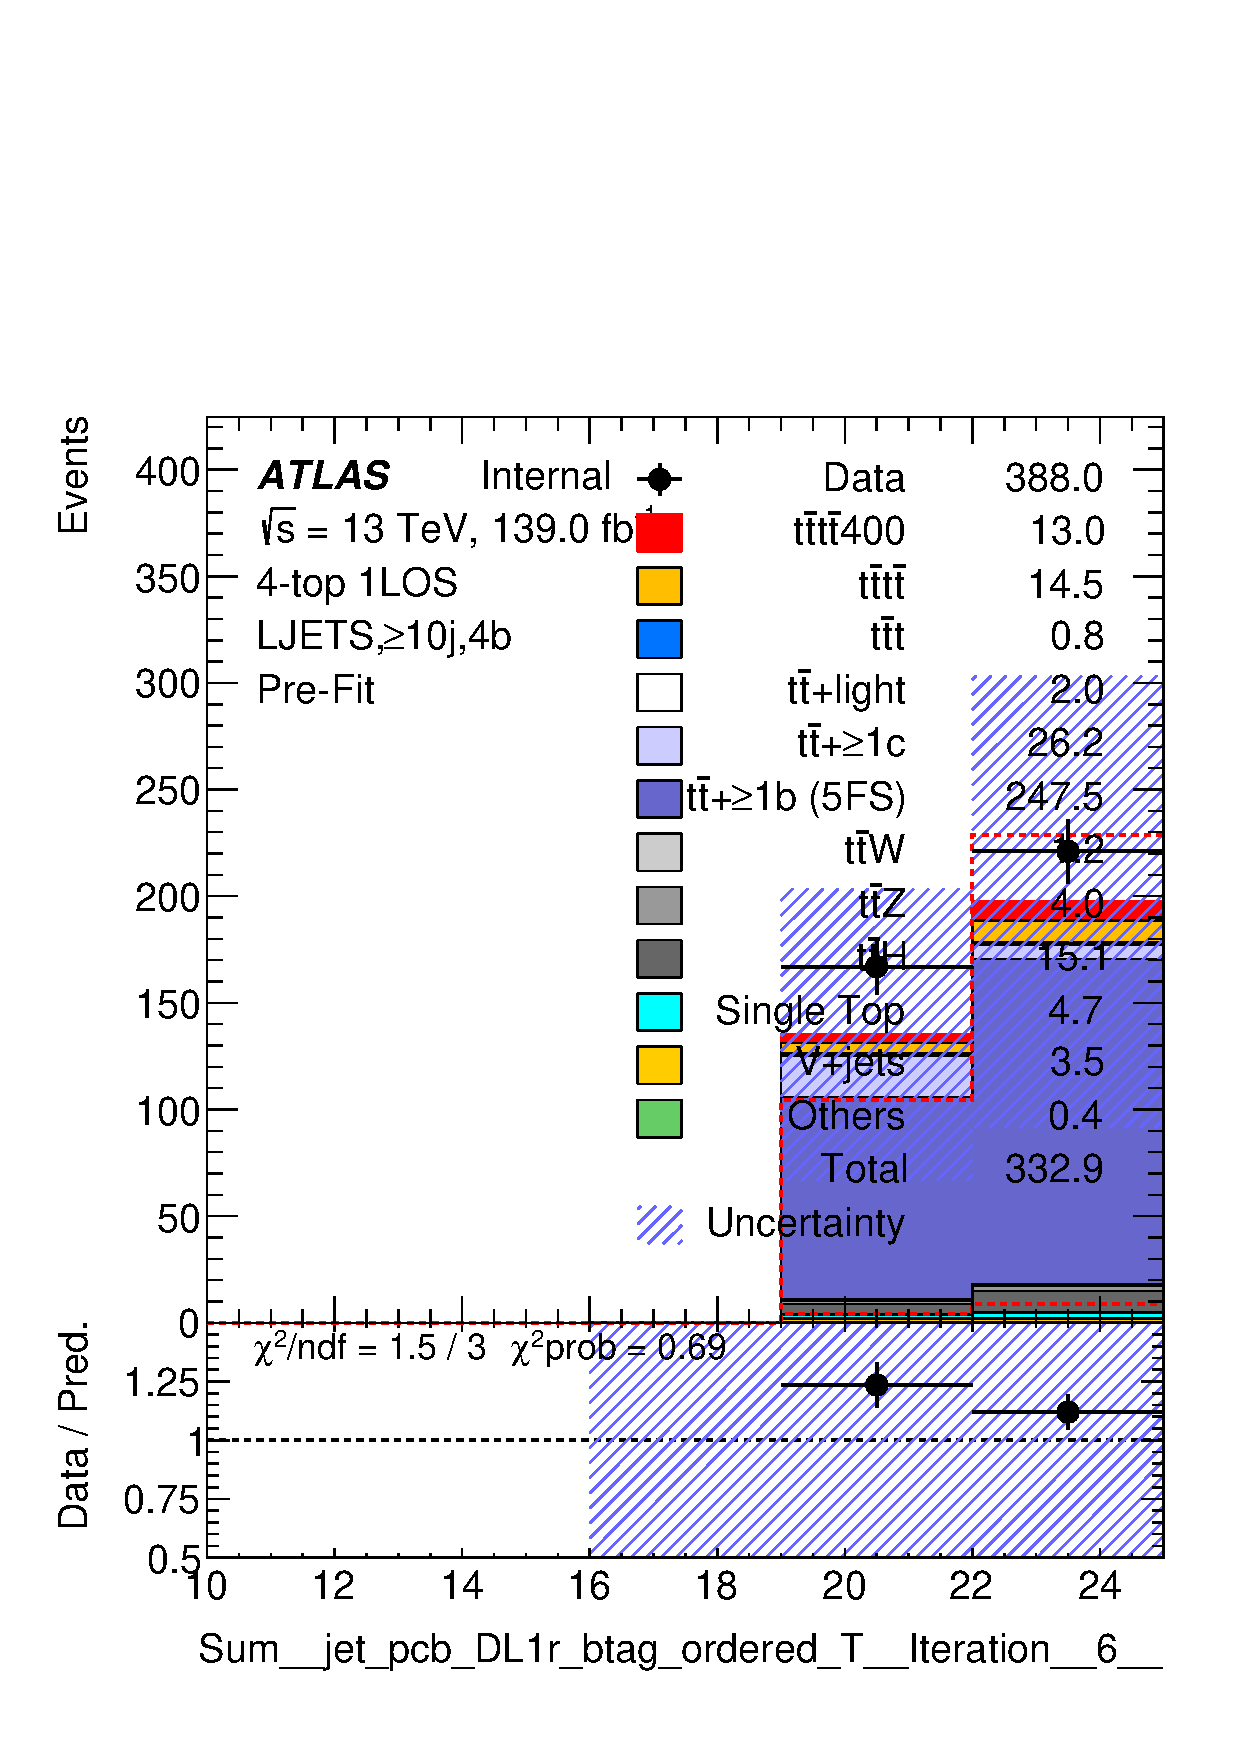
\includegraphics[width=0.23 \textwidth]{figures/fits/GNN/400/all/data_unblindedBonly/Plots/val_ljets_ge10j4b_sum_pcb.pdf} &
        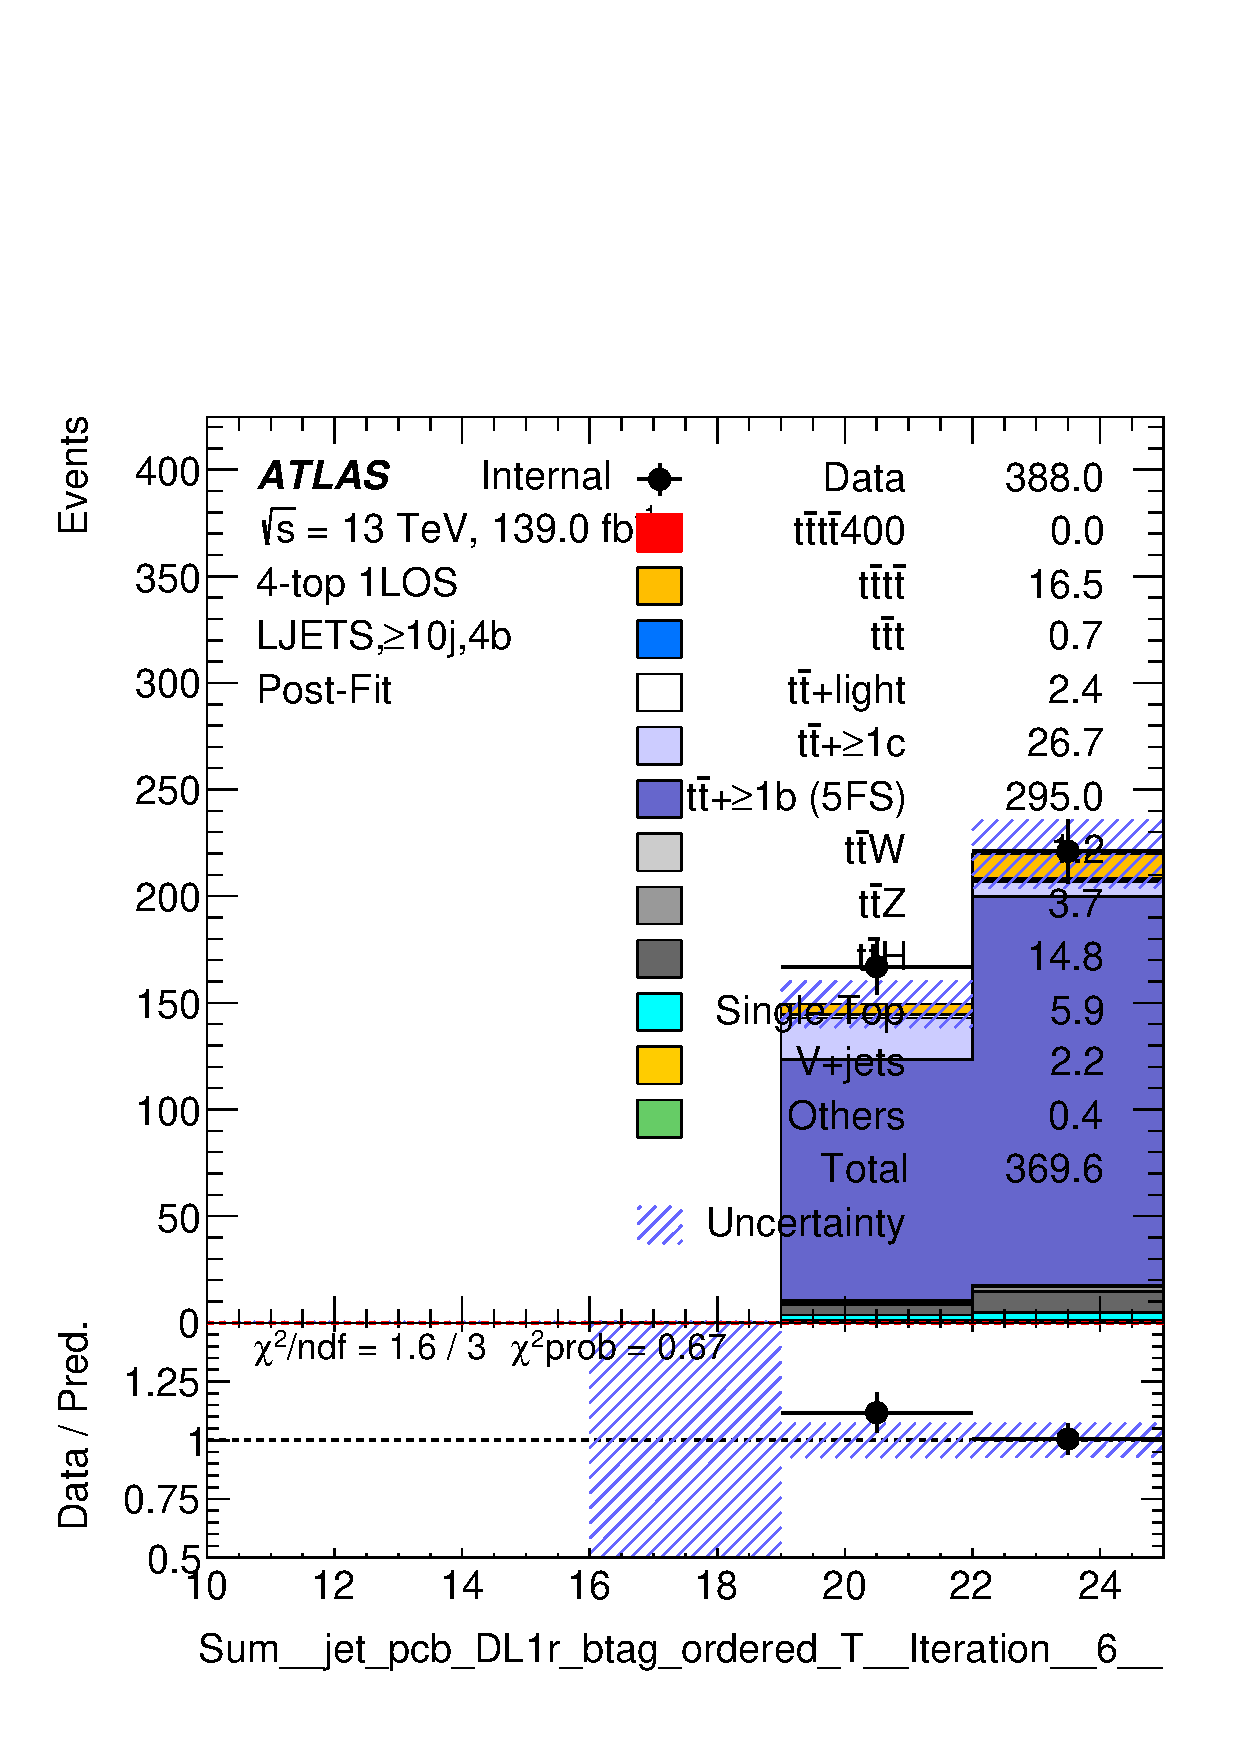
\includegraphics[width=0.23 \textwidth]{figures/fits/GNN/400/all/data_unblindedBonly/Plots/val_ljets_ge10j4b_sum_pcb_postFit.pdf} \\

        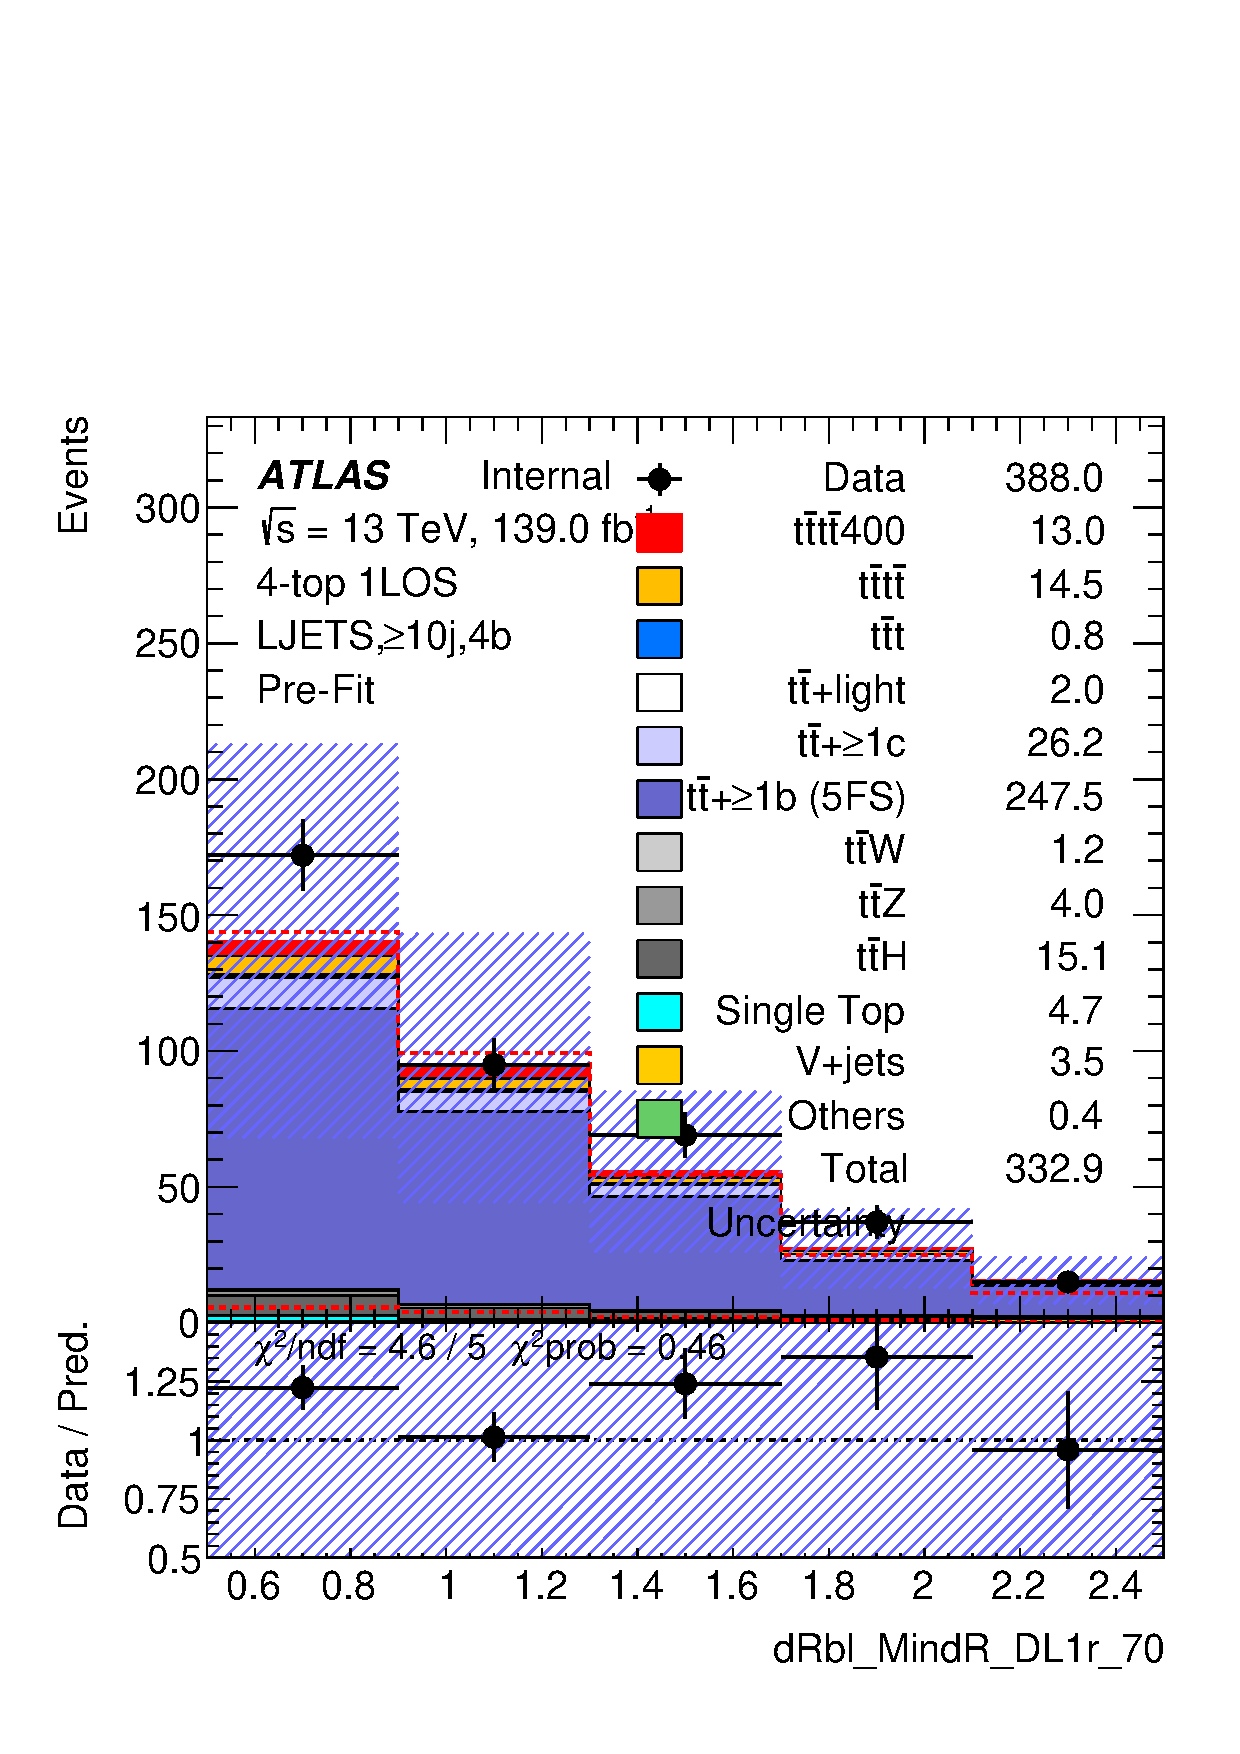
\includegraphics[width=0.23 \textwidth]{figures/fits/GNN/400/all/data_unblindedBonly/Plots/val_ljets_ge10j4b_dRbl_MindR_DL1r_70.pdf} &
        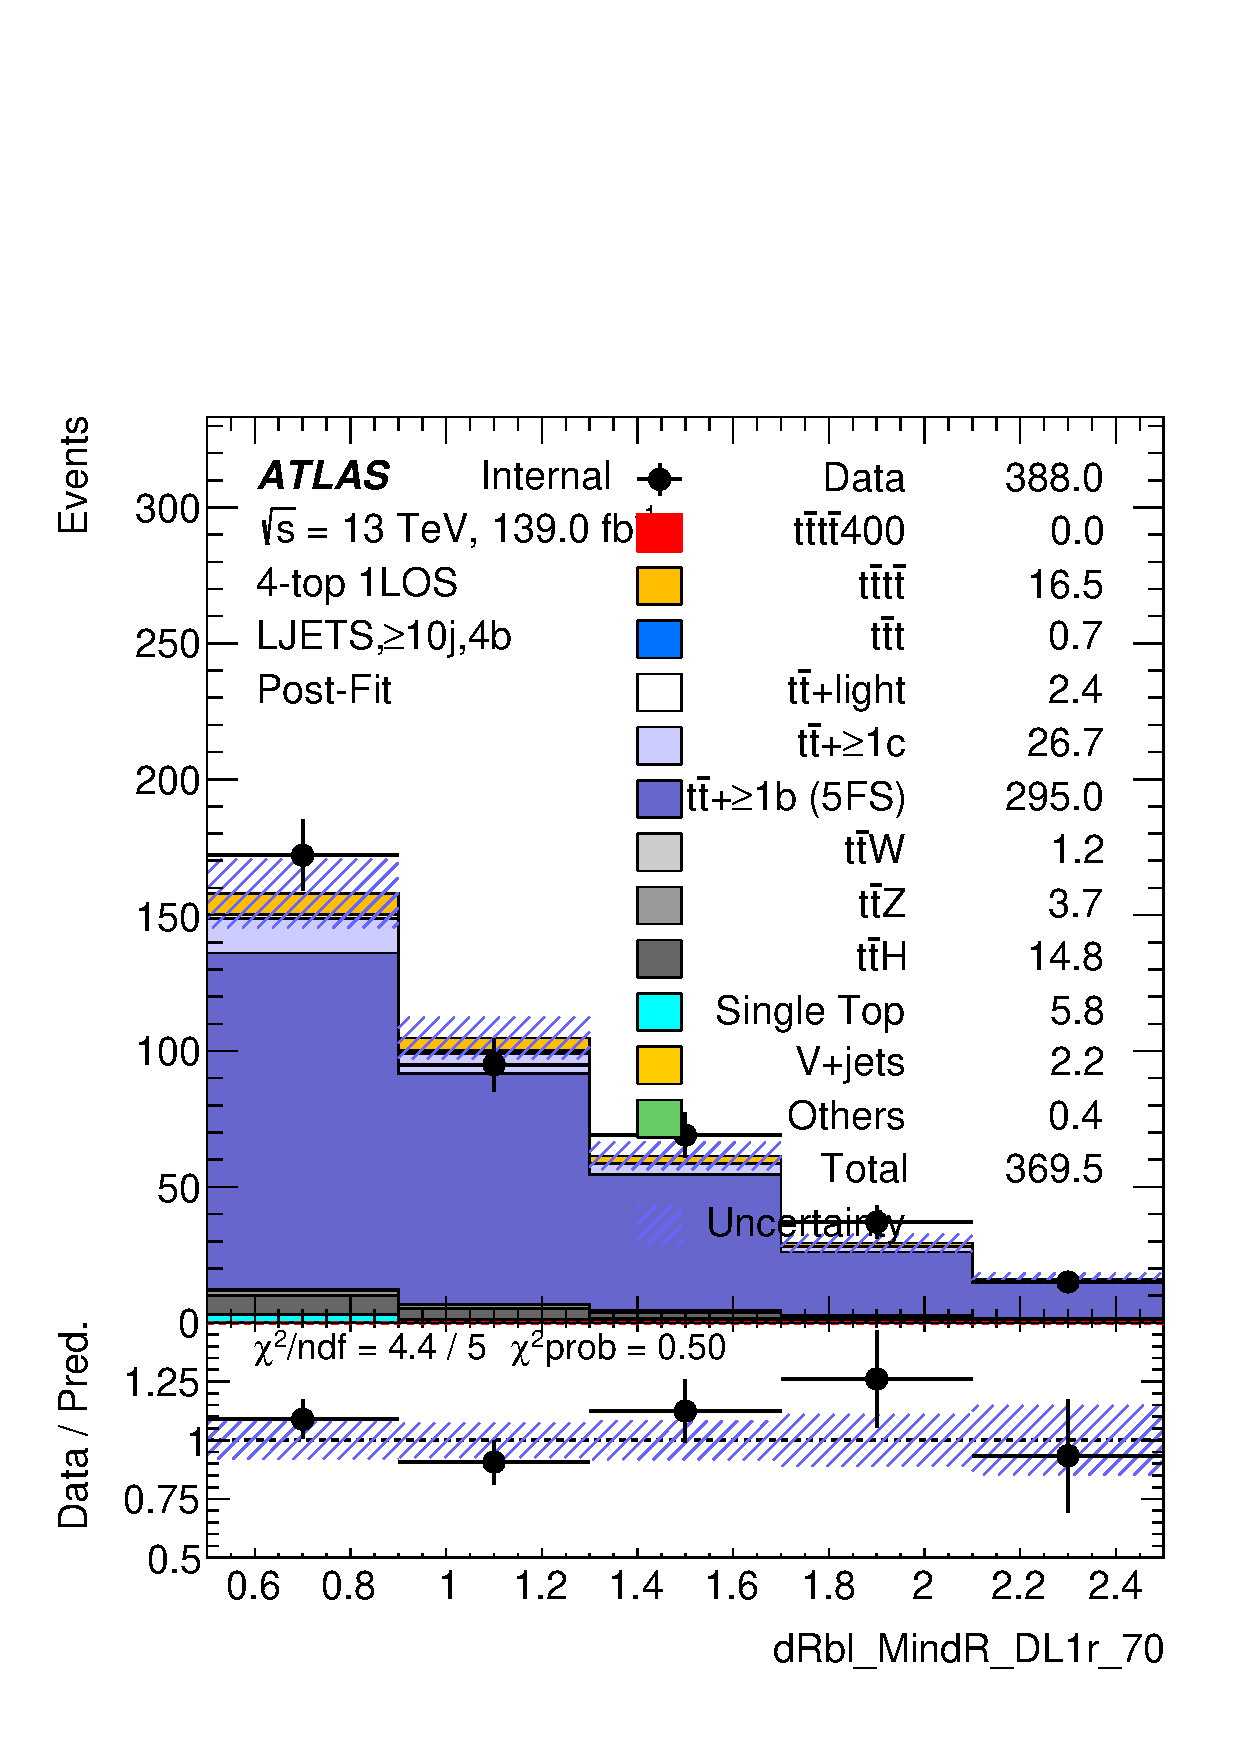
\includegraphics[width=0.23 \textwidth]{figures/fits/GNN/400/all/data_unblindedBonly/Plots/val_ljets_ge10j4b_dRbl_MindR_DL1r_70_postFit.pdf} &
        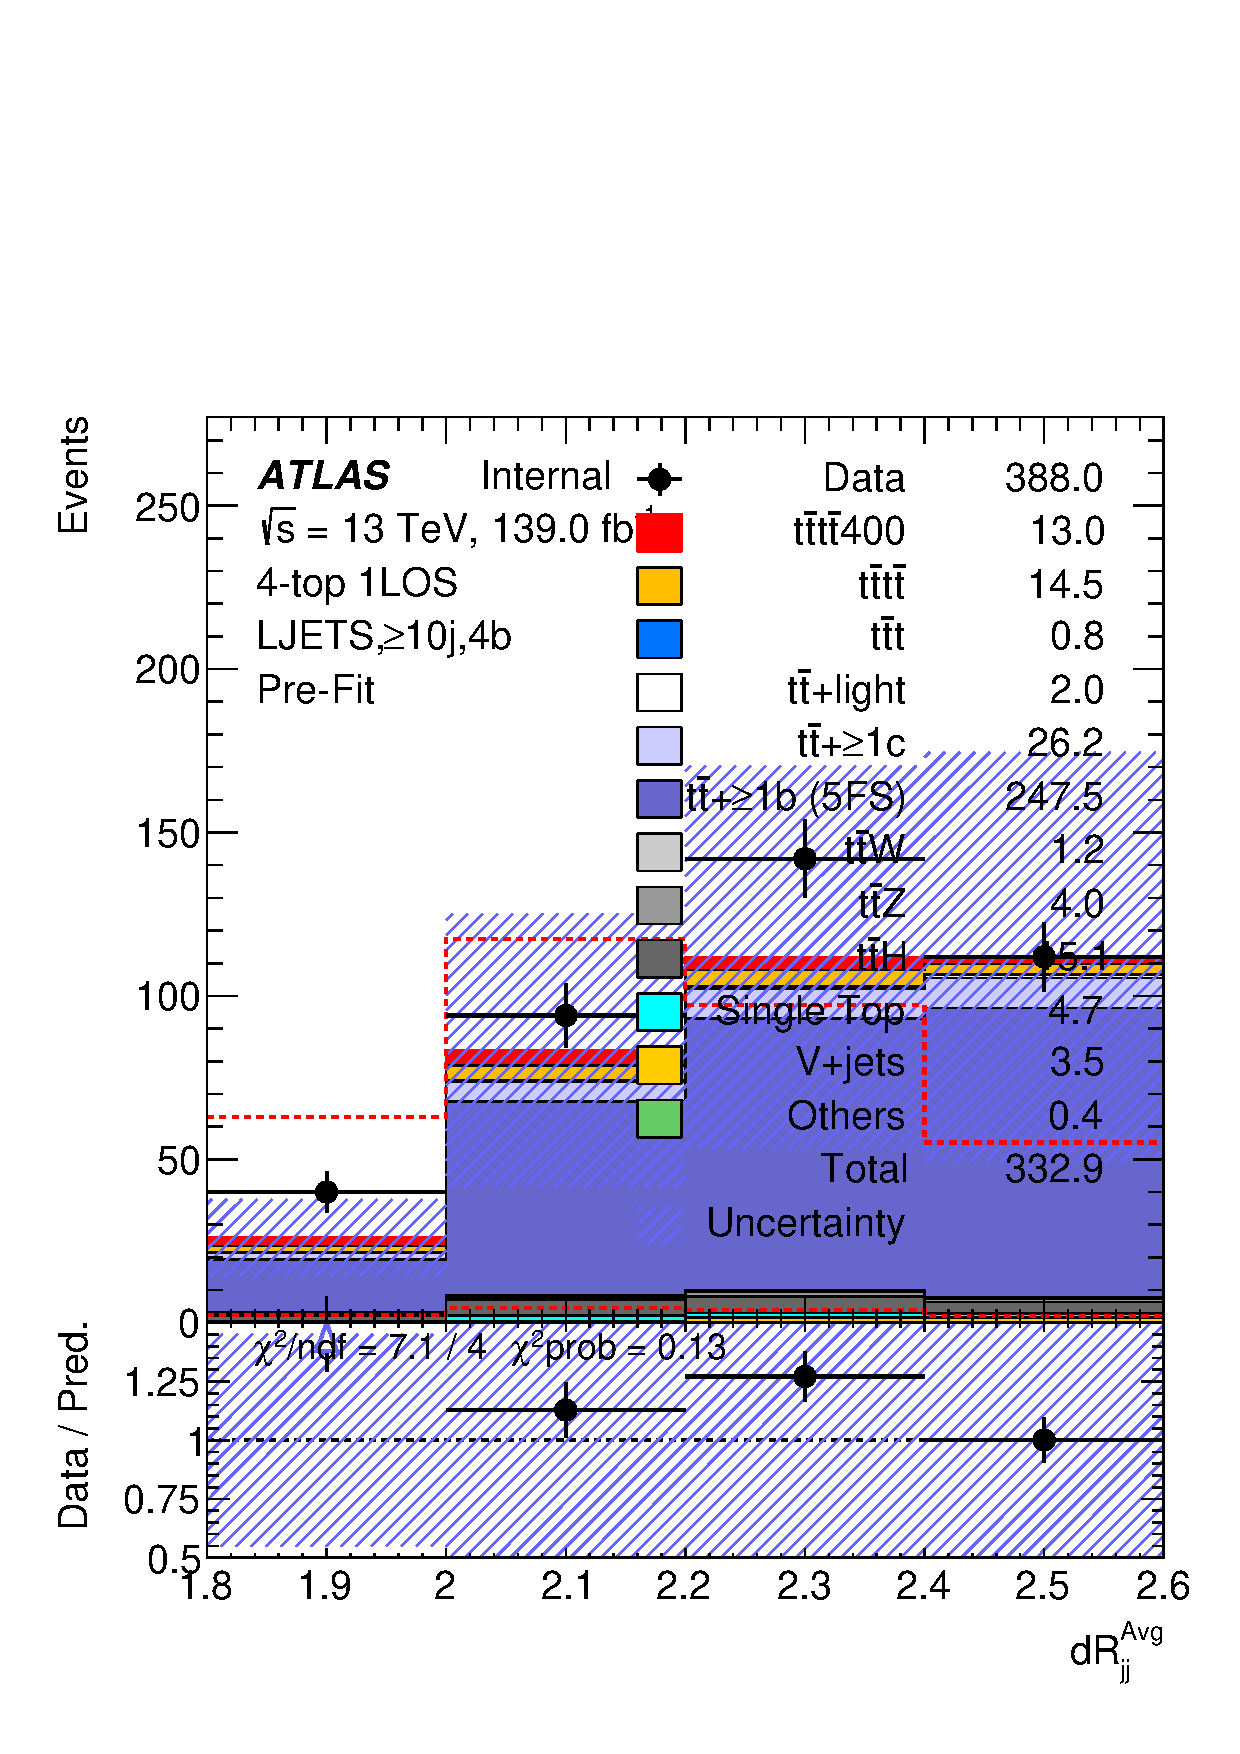
\includegraphics[width=0.23 \textwidth]{figures/fits/GNN/400/all/data_unblindedBonly/Plots/val_ljets_ge10j4b_dRjj_Avg.pdf} &
        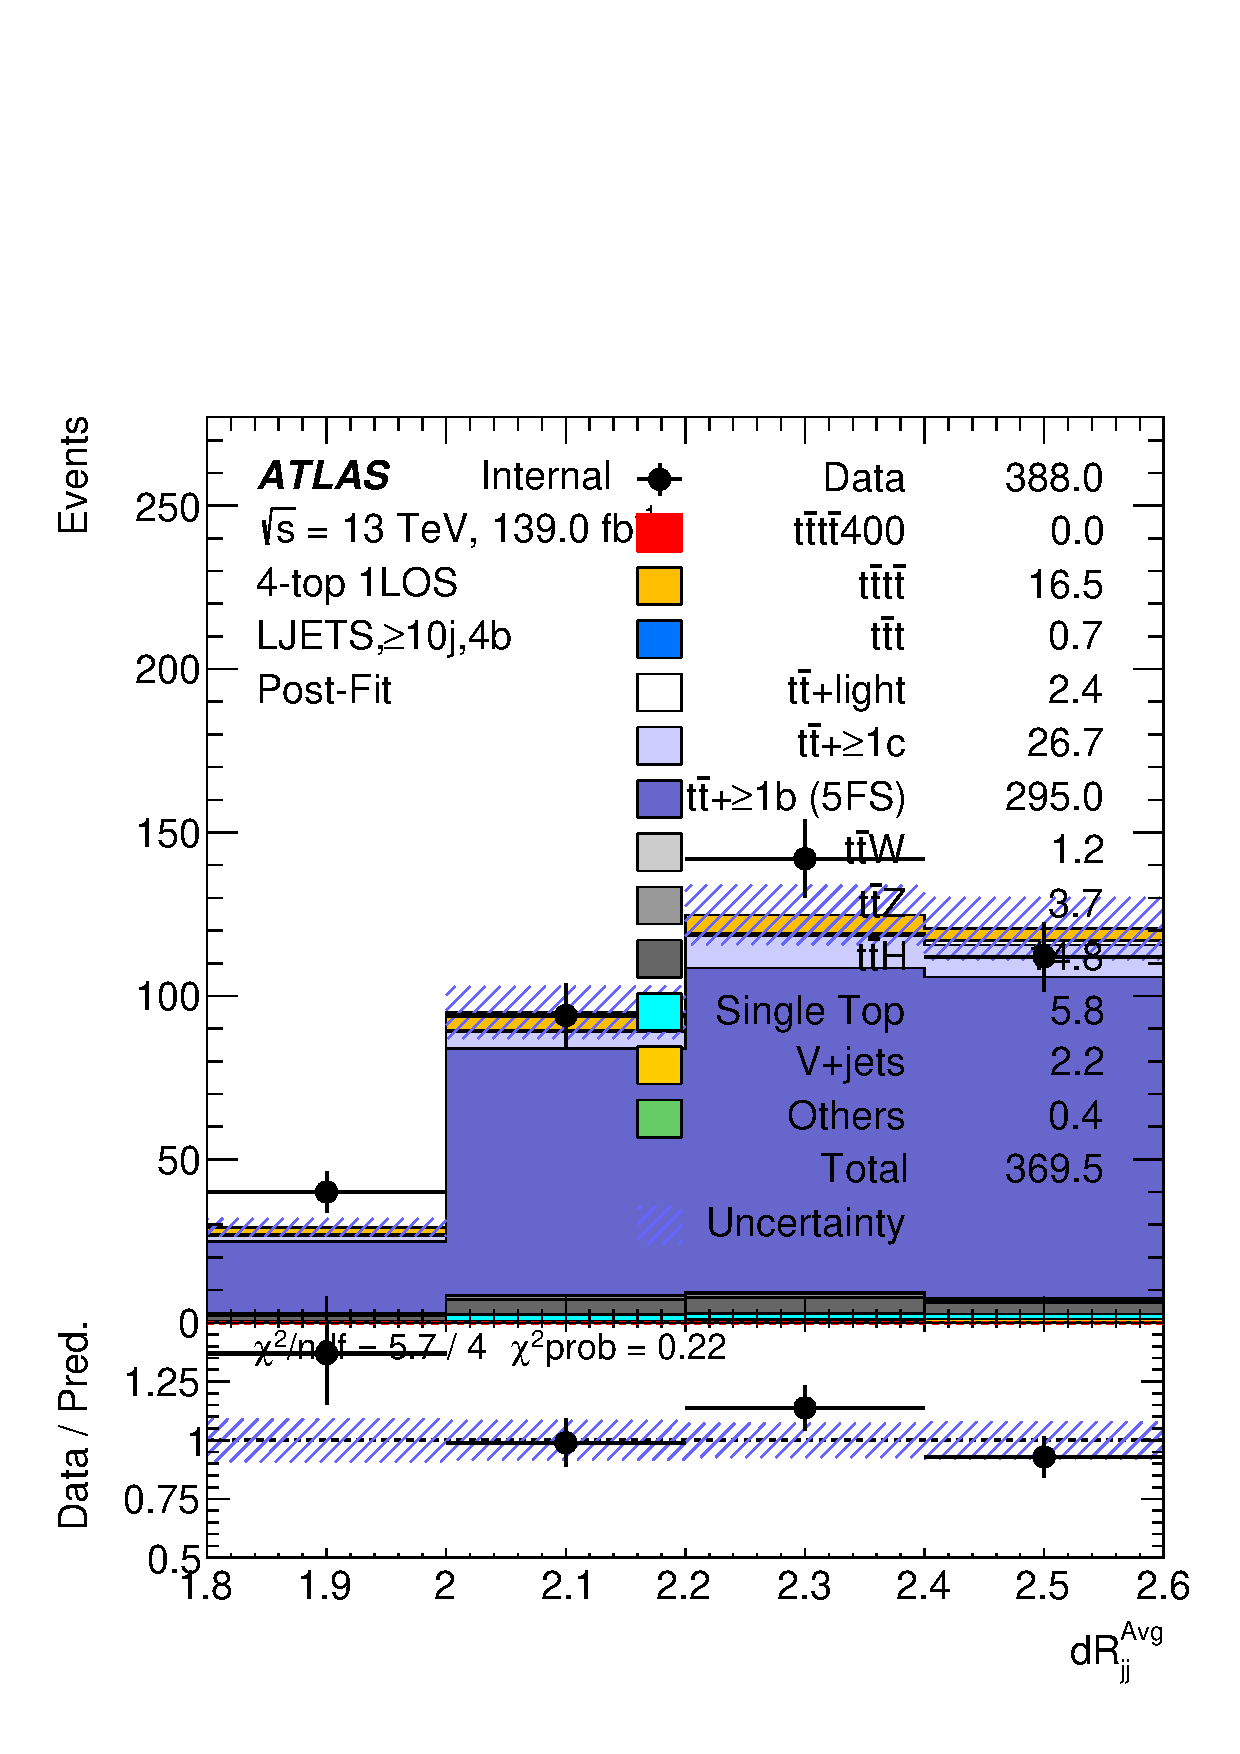
\includegraphics[width=0.23 \textwidth]{figures/fits/GNN/400/all/data_unblindedBonly/Plots/val_ljets_ge10j4b_dRjj_Avg_postFit.pdf} \\

        \end{tabular}
        \end{center}

\caption{\label{GNN_input_val_1}Pre-fit(left) and Post-fit(right) distributions for GNN input variables in the ge10j4b region.}
\end{figure}

\begin{figure}

        \begin{center} \setlength{\tabcolsep}{2.5pt}\footnotesize
        \begin{tabular}{cccc}

        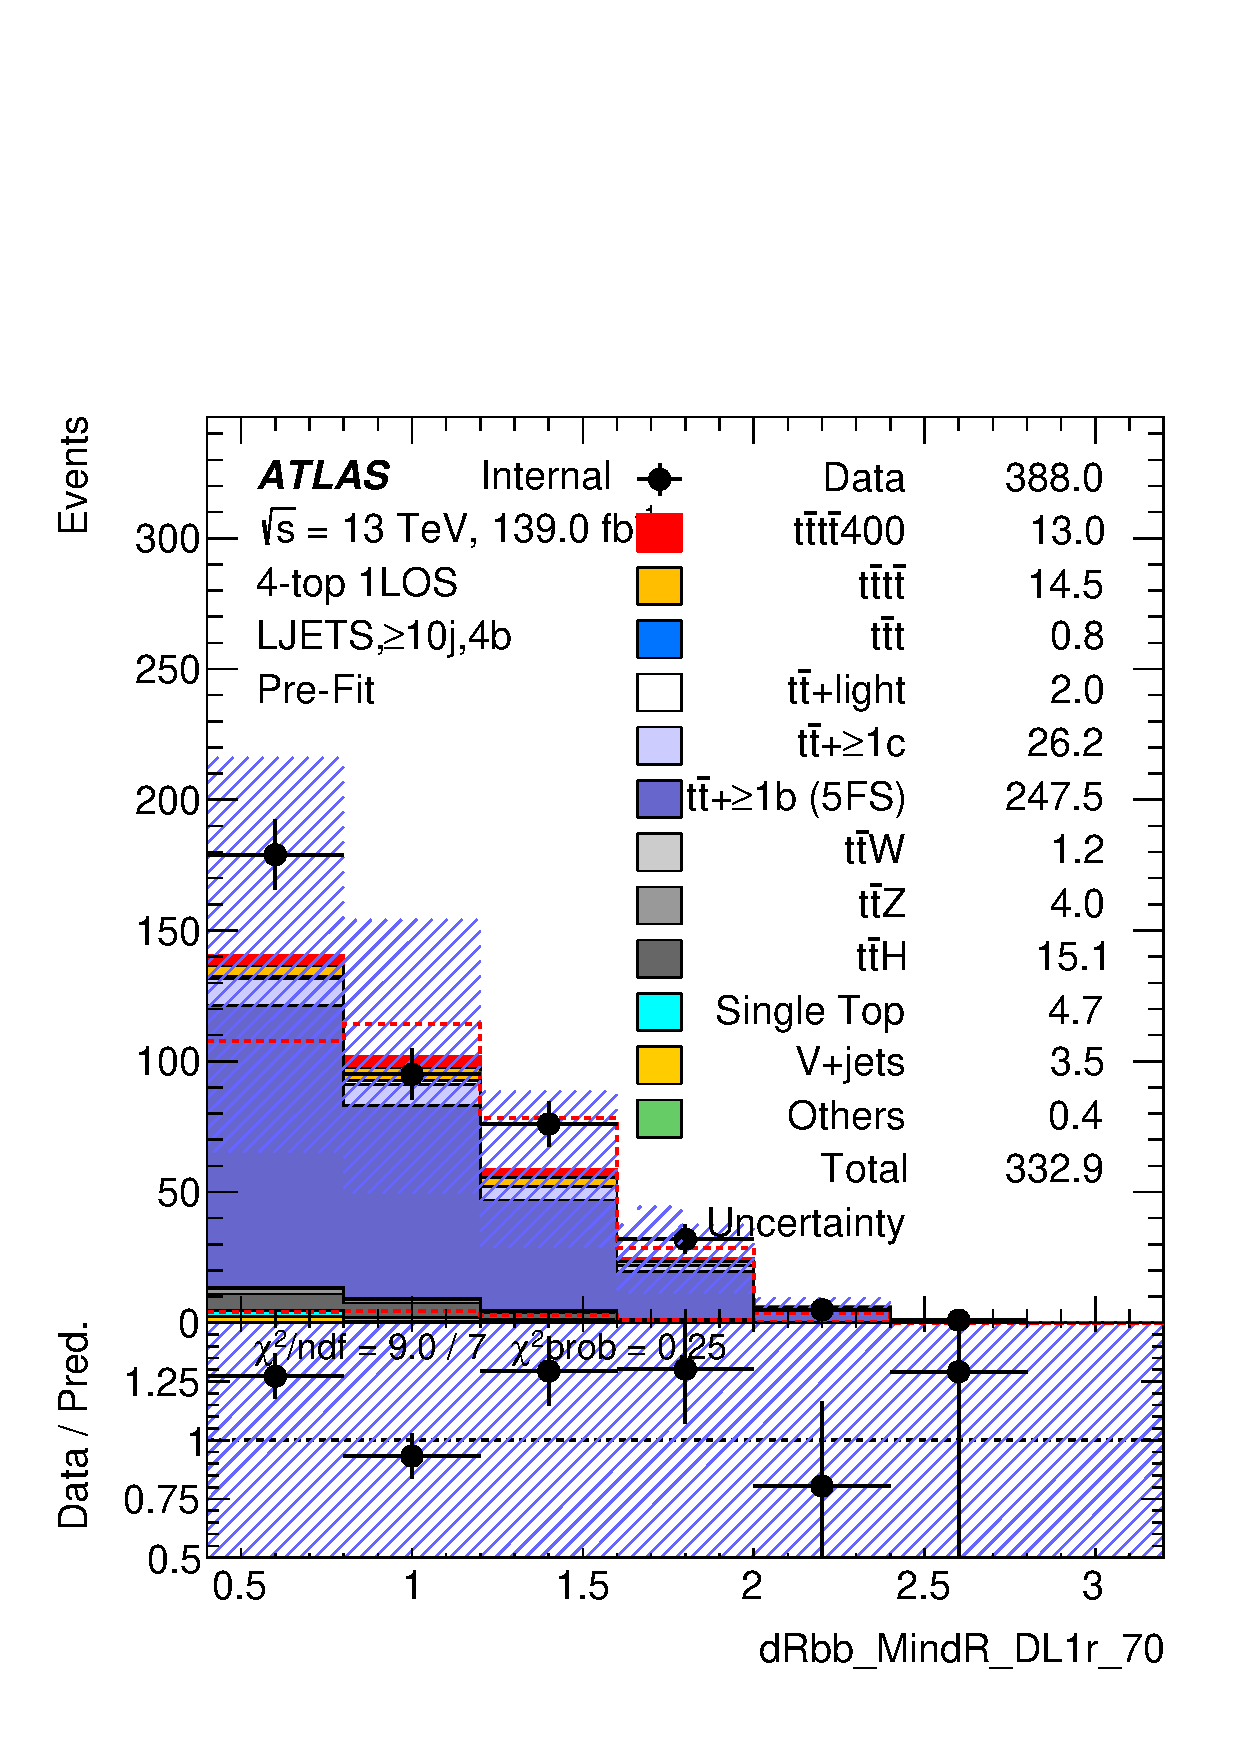
\includegraphics[width=0.23 \textwidth]{figures/fits/GNN/400/all/data_unblindedBonly/Plots/val_ljets_ge10j4b_dRbb_MindR_DL1r_70.pdf} &
        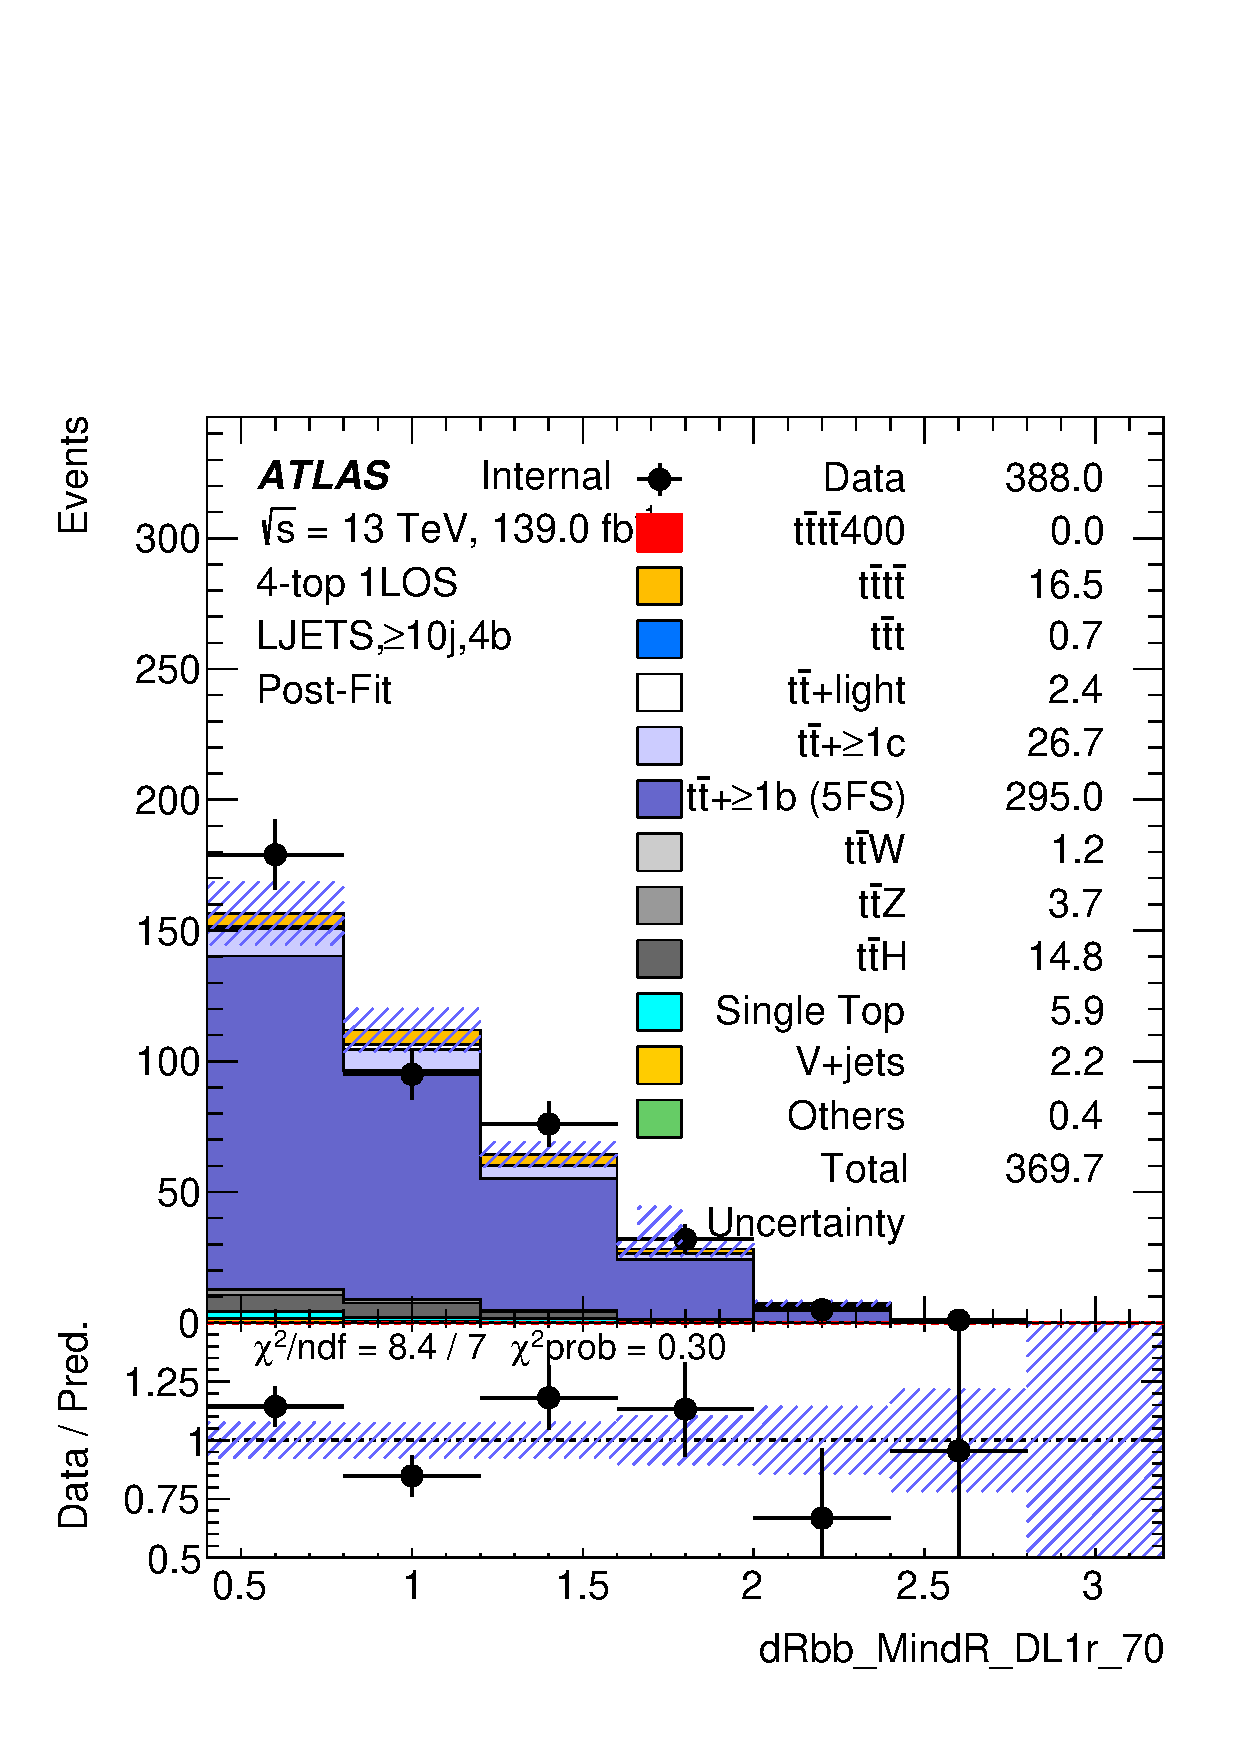
\includegraphics[width=0.23 \textwidth]{figures/fits/GNN/400/all/data_unblindedBonly/Plots/val_ljets_ge10j4b_dRbb_MindR_DL1r_70_postFit.pdf} &
        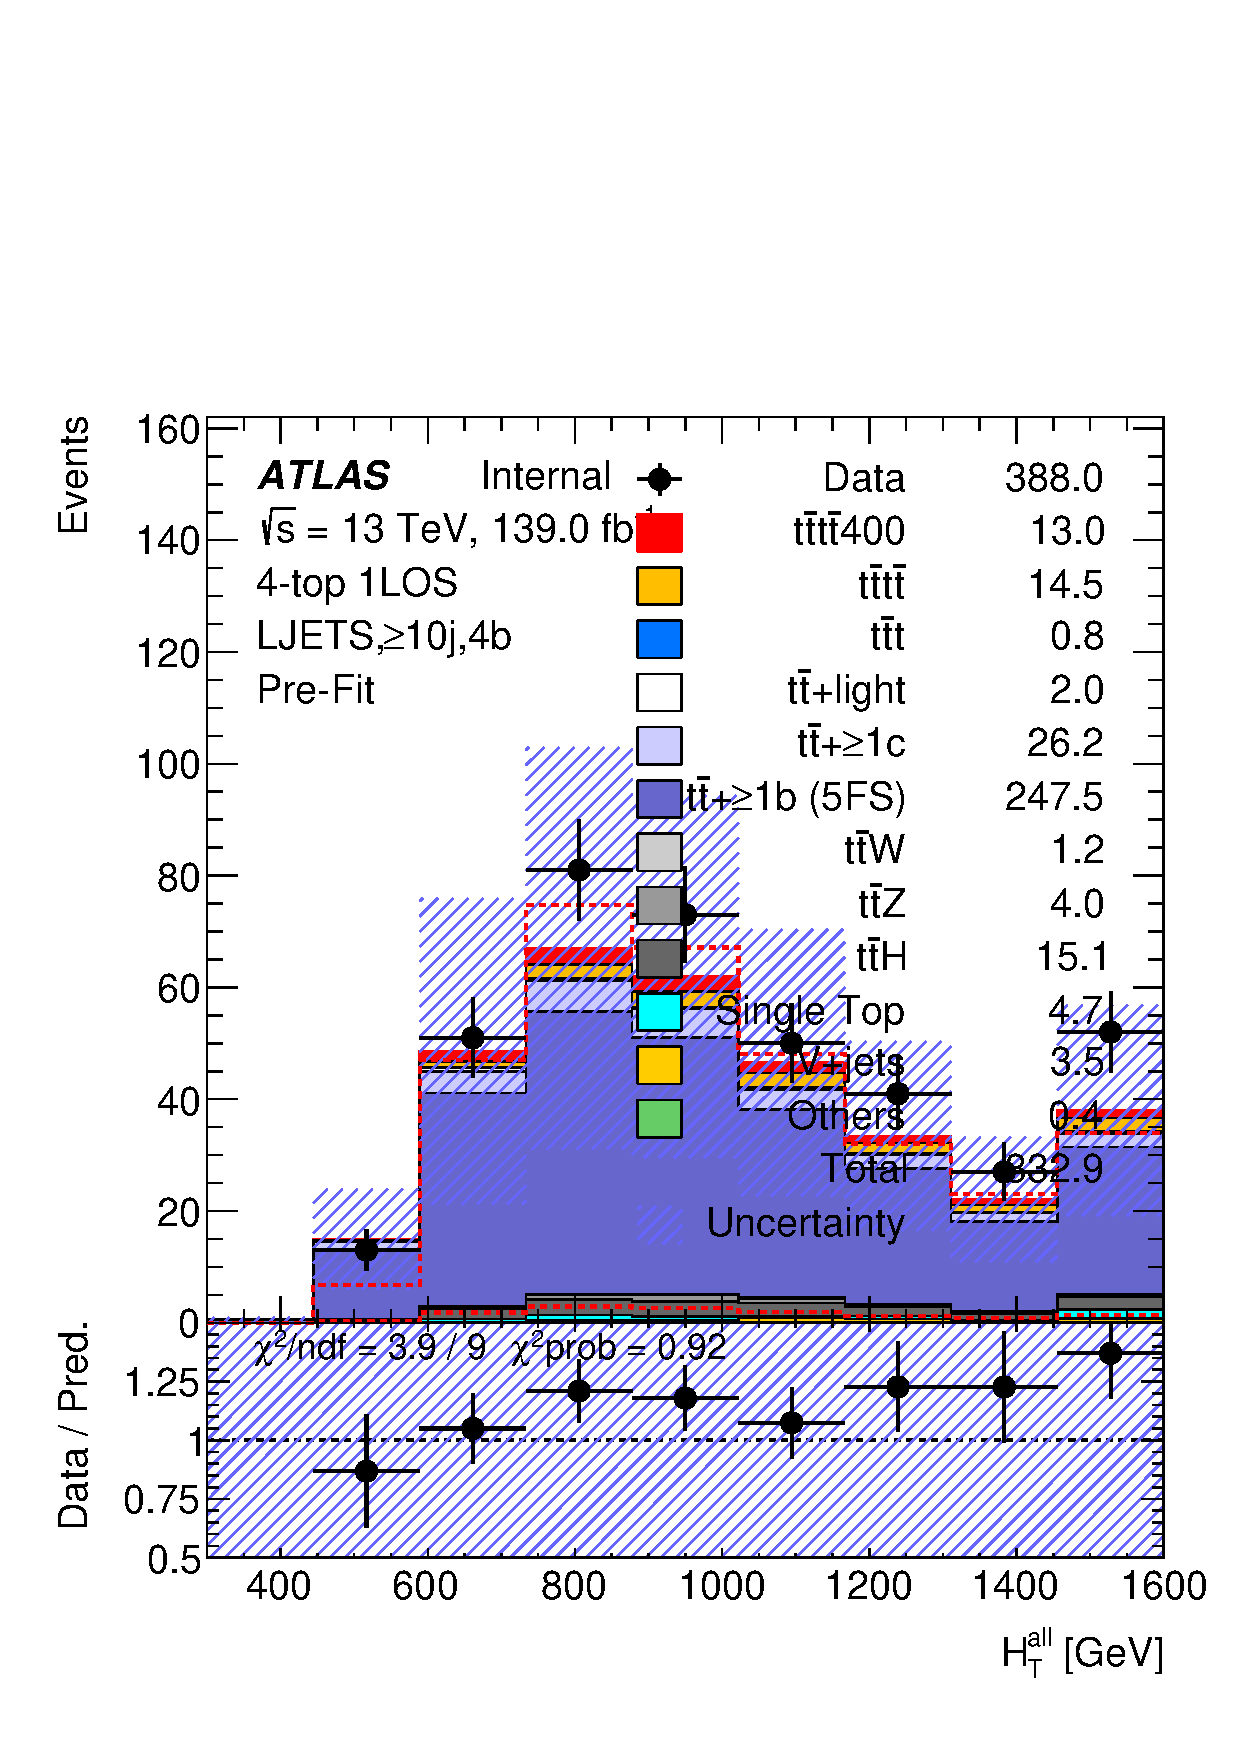
\includegraphics[width=0.23 \textwidth]{figures/fits/GNN/400/all/data_unblindedBonly/Plots/val_ljets_ge10j4b_HT_all.pdf} &
        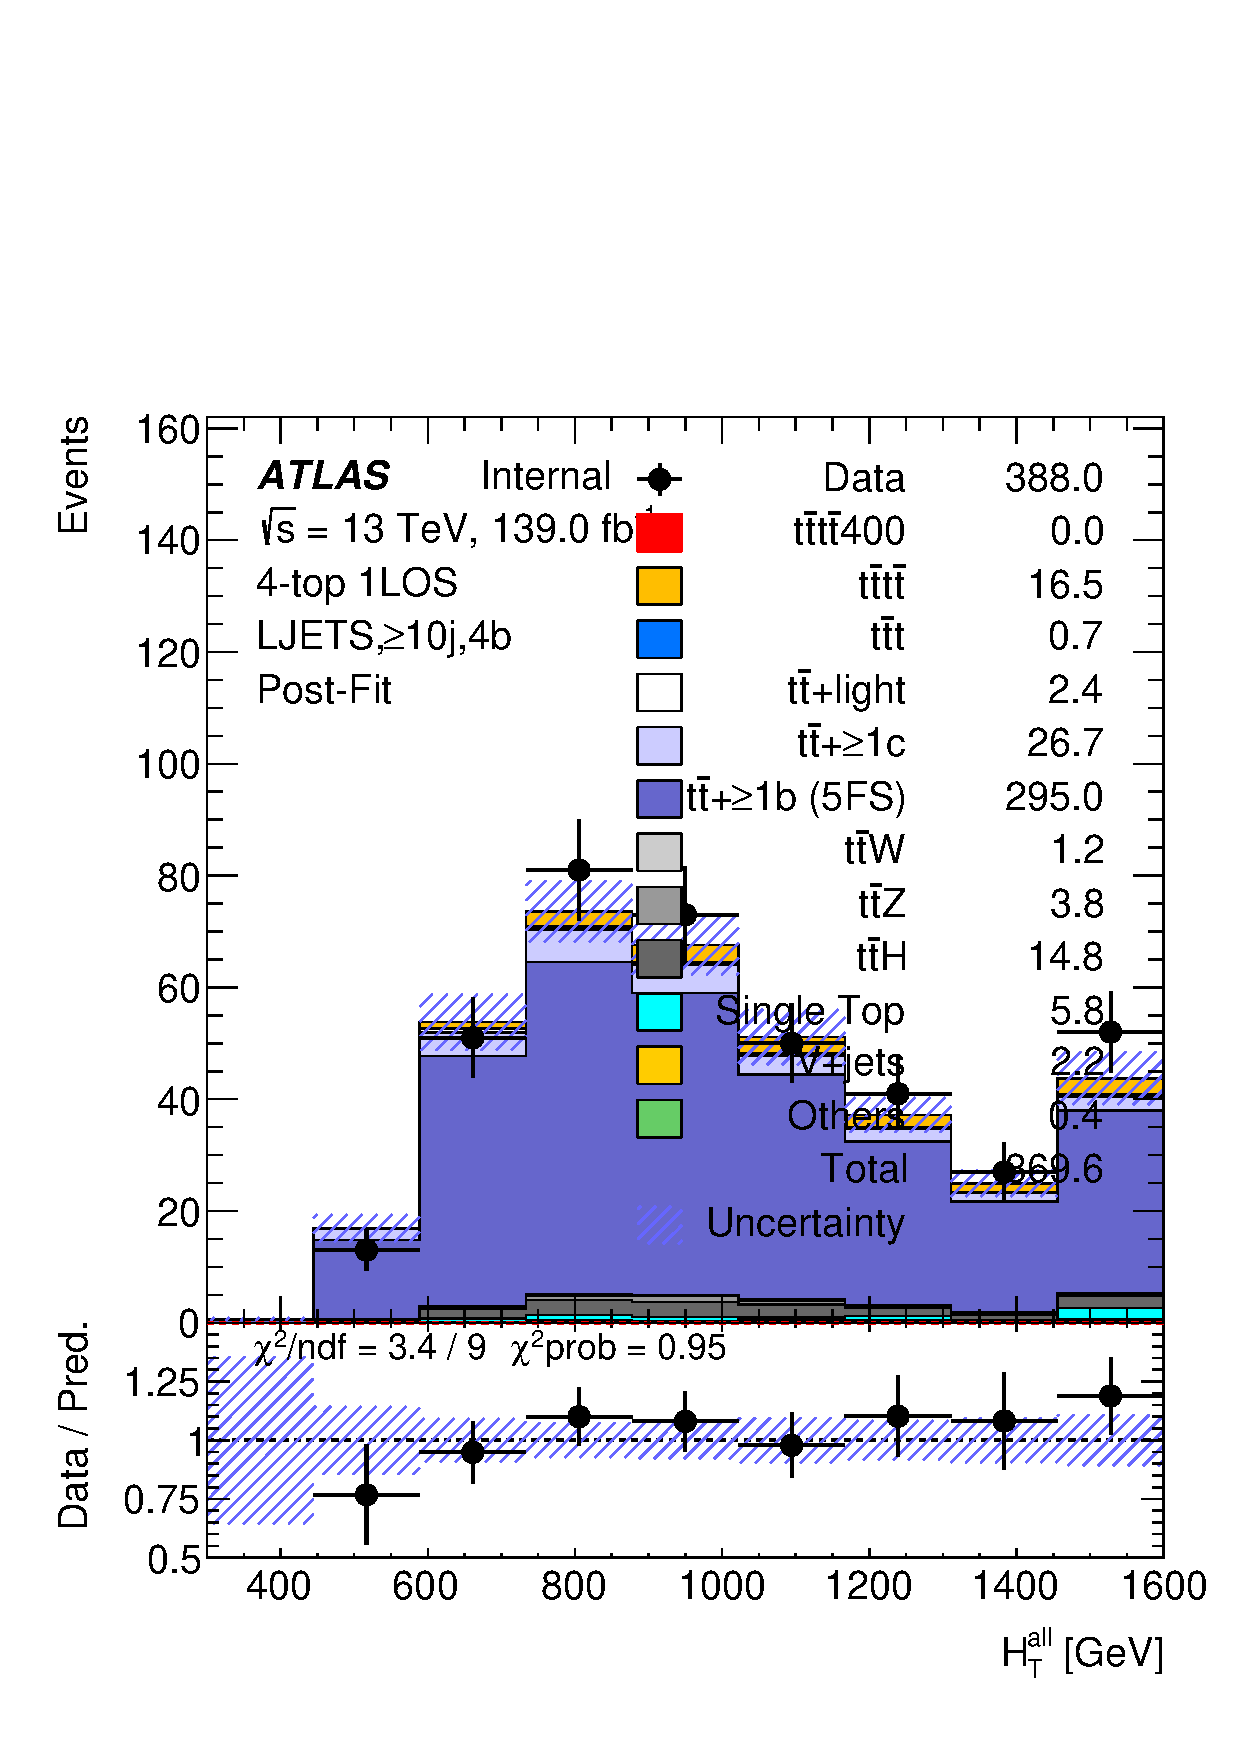
\includegraphics[width=0.23 \textwidth]{figures/fits/GNN/400/all/data_unblindedBonly/Plots/val_ljets_ge10j4b_HT_all_postFit.pdf} \\

        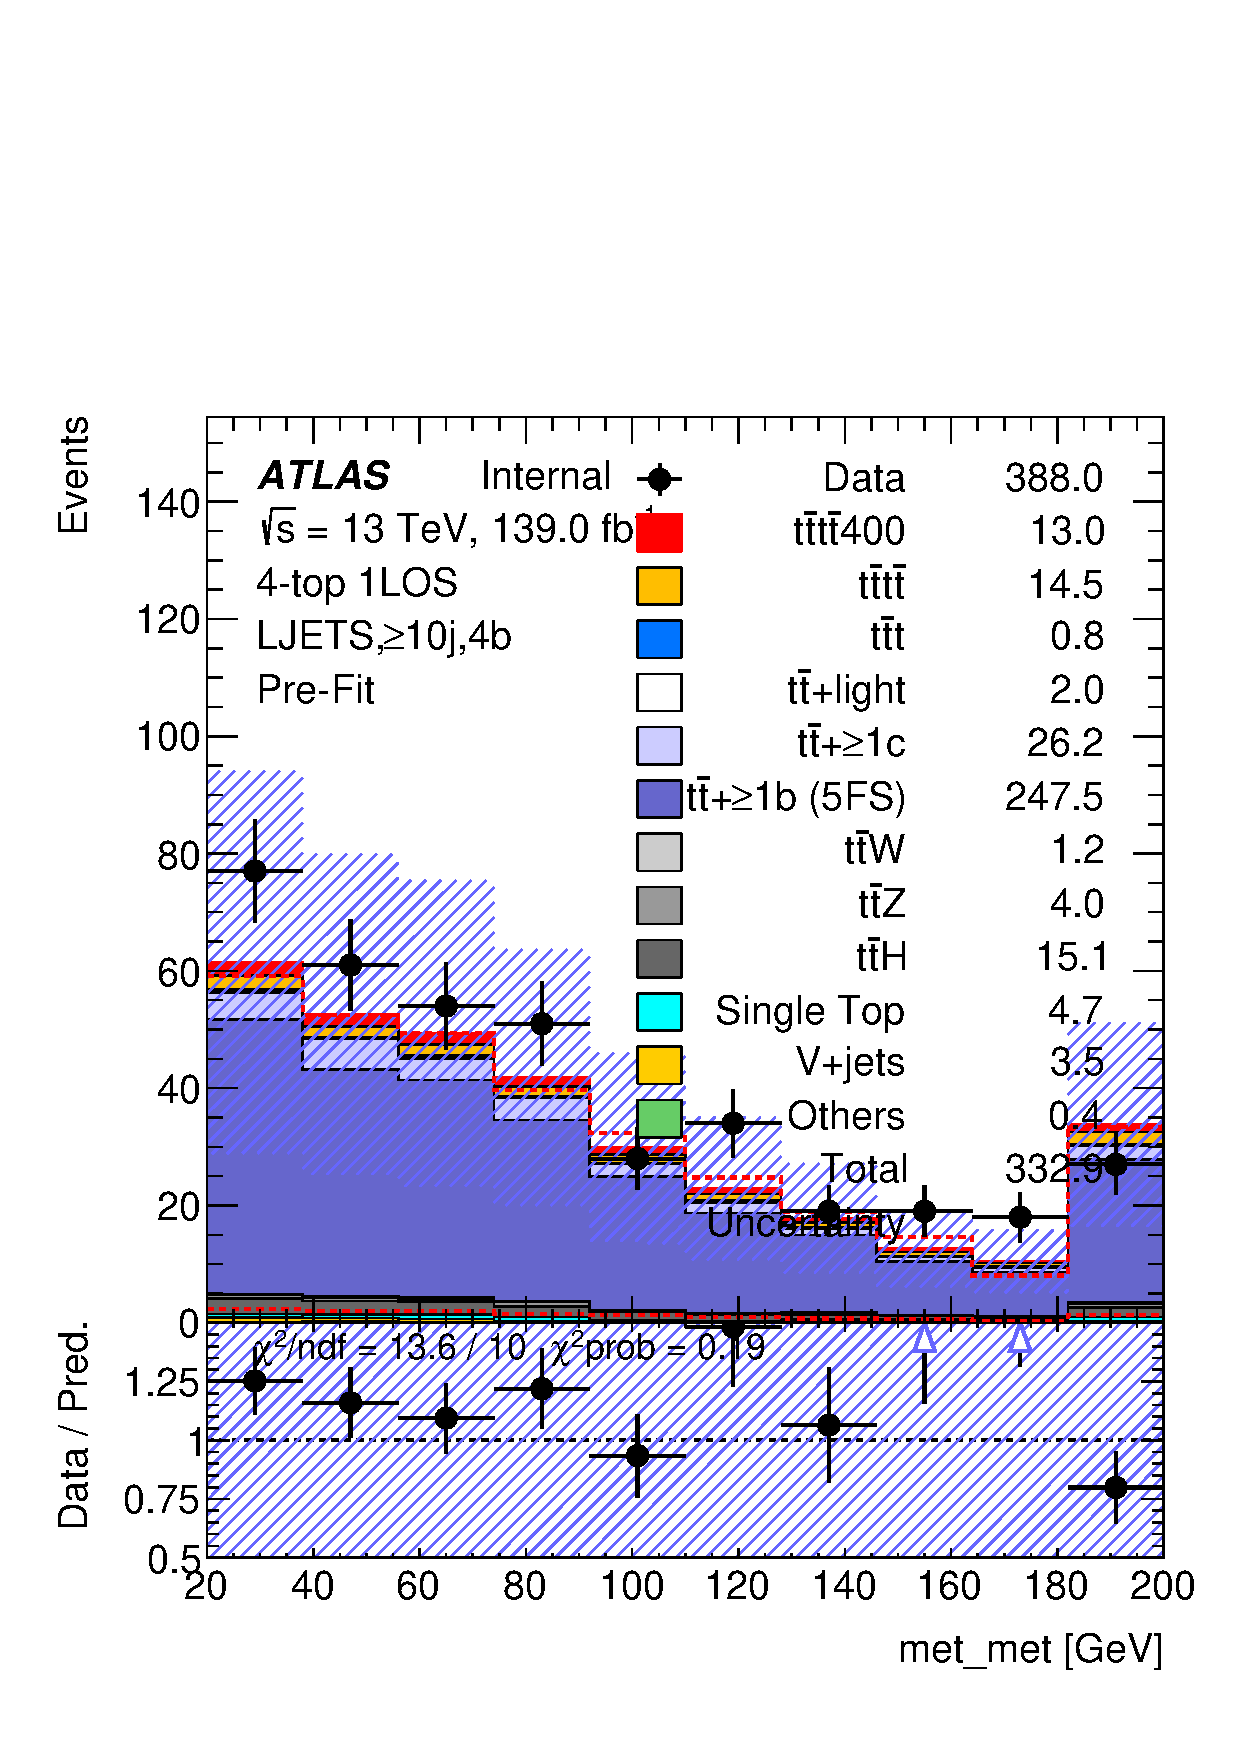
\includegraphics[width=0.23 \textwidth]{figures/fits/GNN/400/all/data_unblindedBonly/Plots/val_ljets_ge10j4b_met.pdf} &
        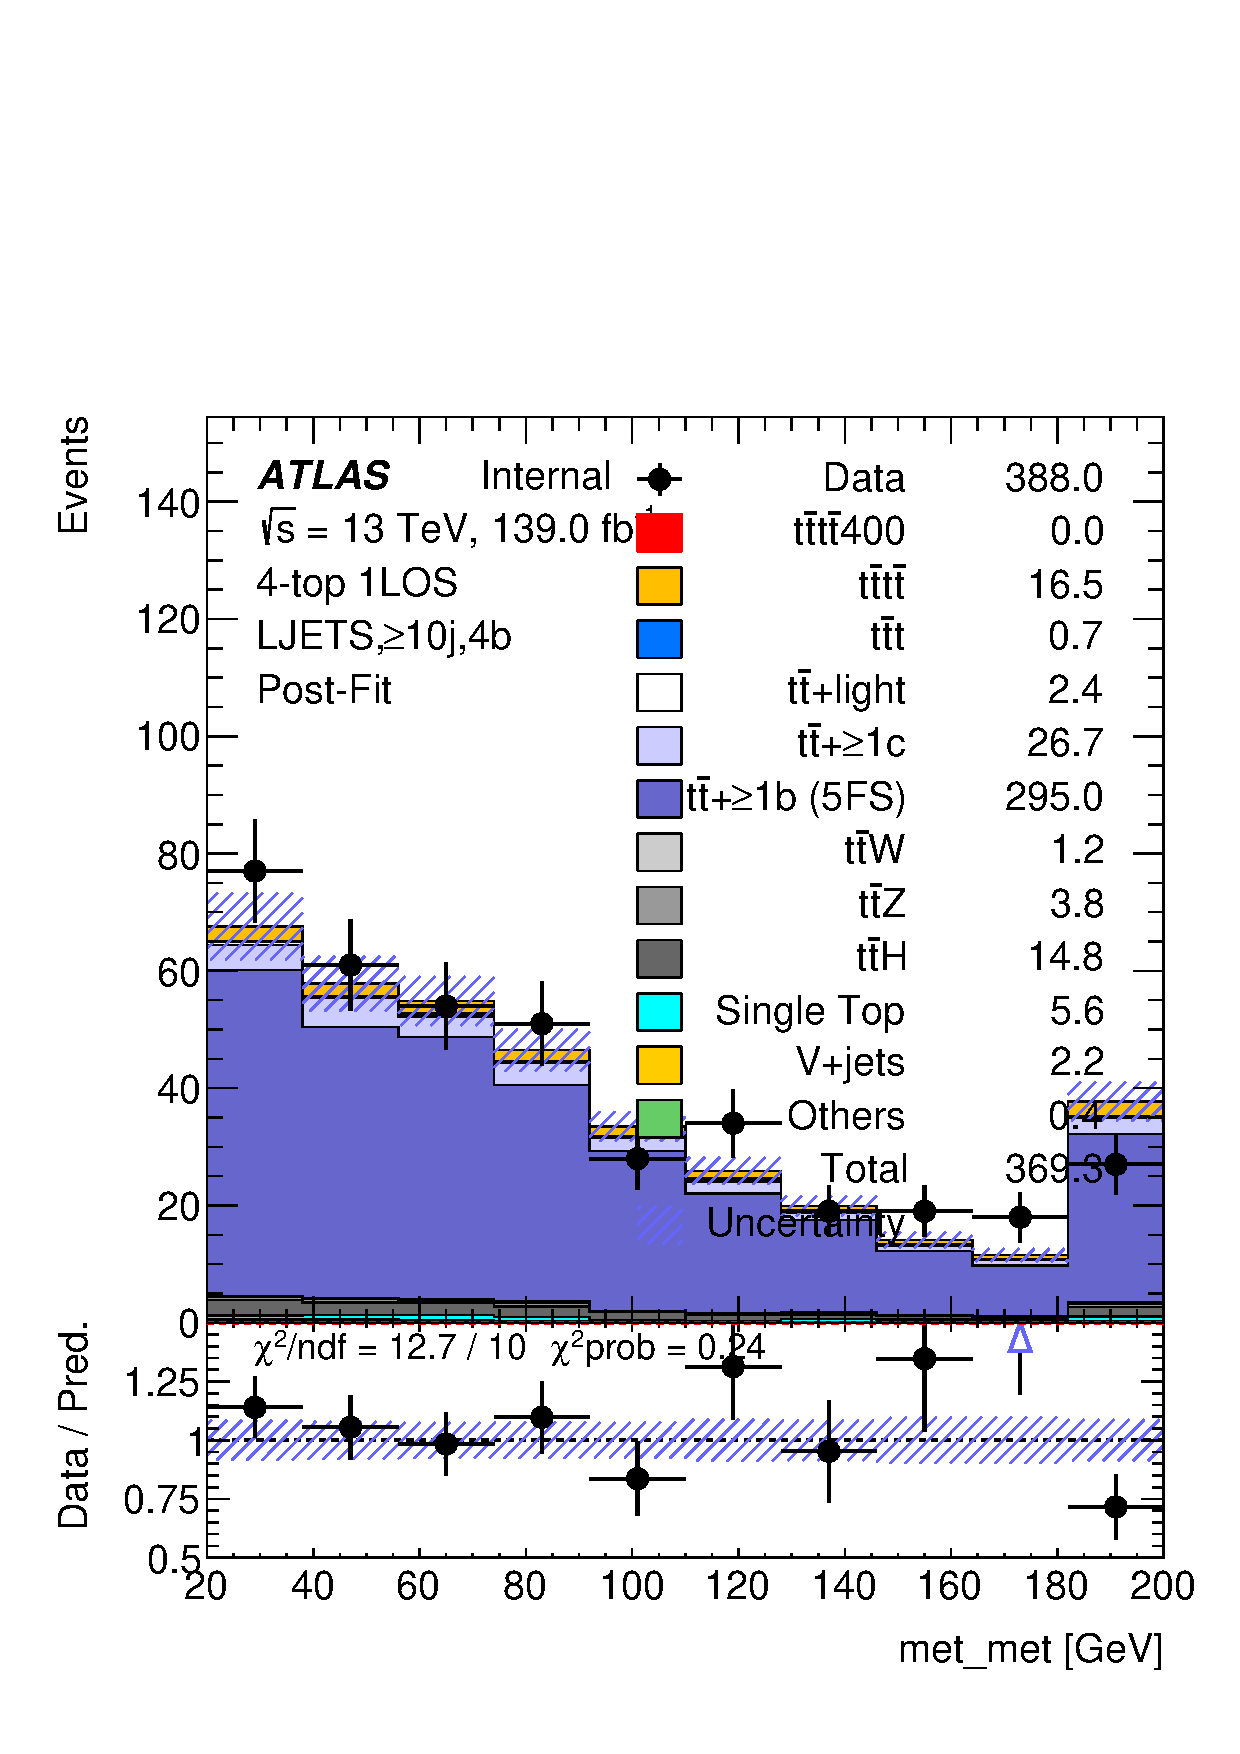
\includegraphics[width=0.23 \textwidth]{figures/fits/GNN/400/all/data_unblindedBonly/Plots/val_ljets_ge10j4b_met_postFit.pdf} &
        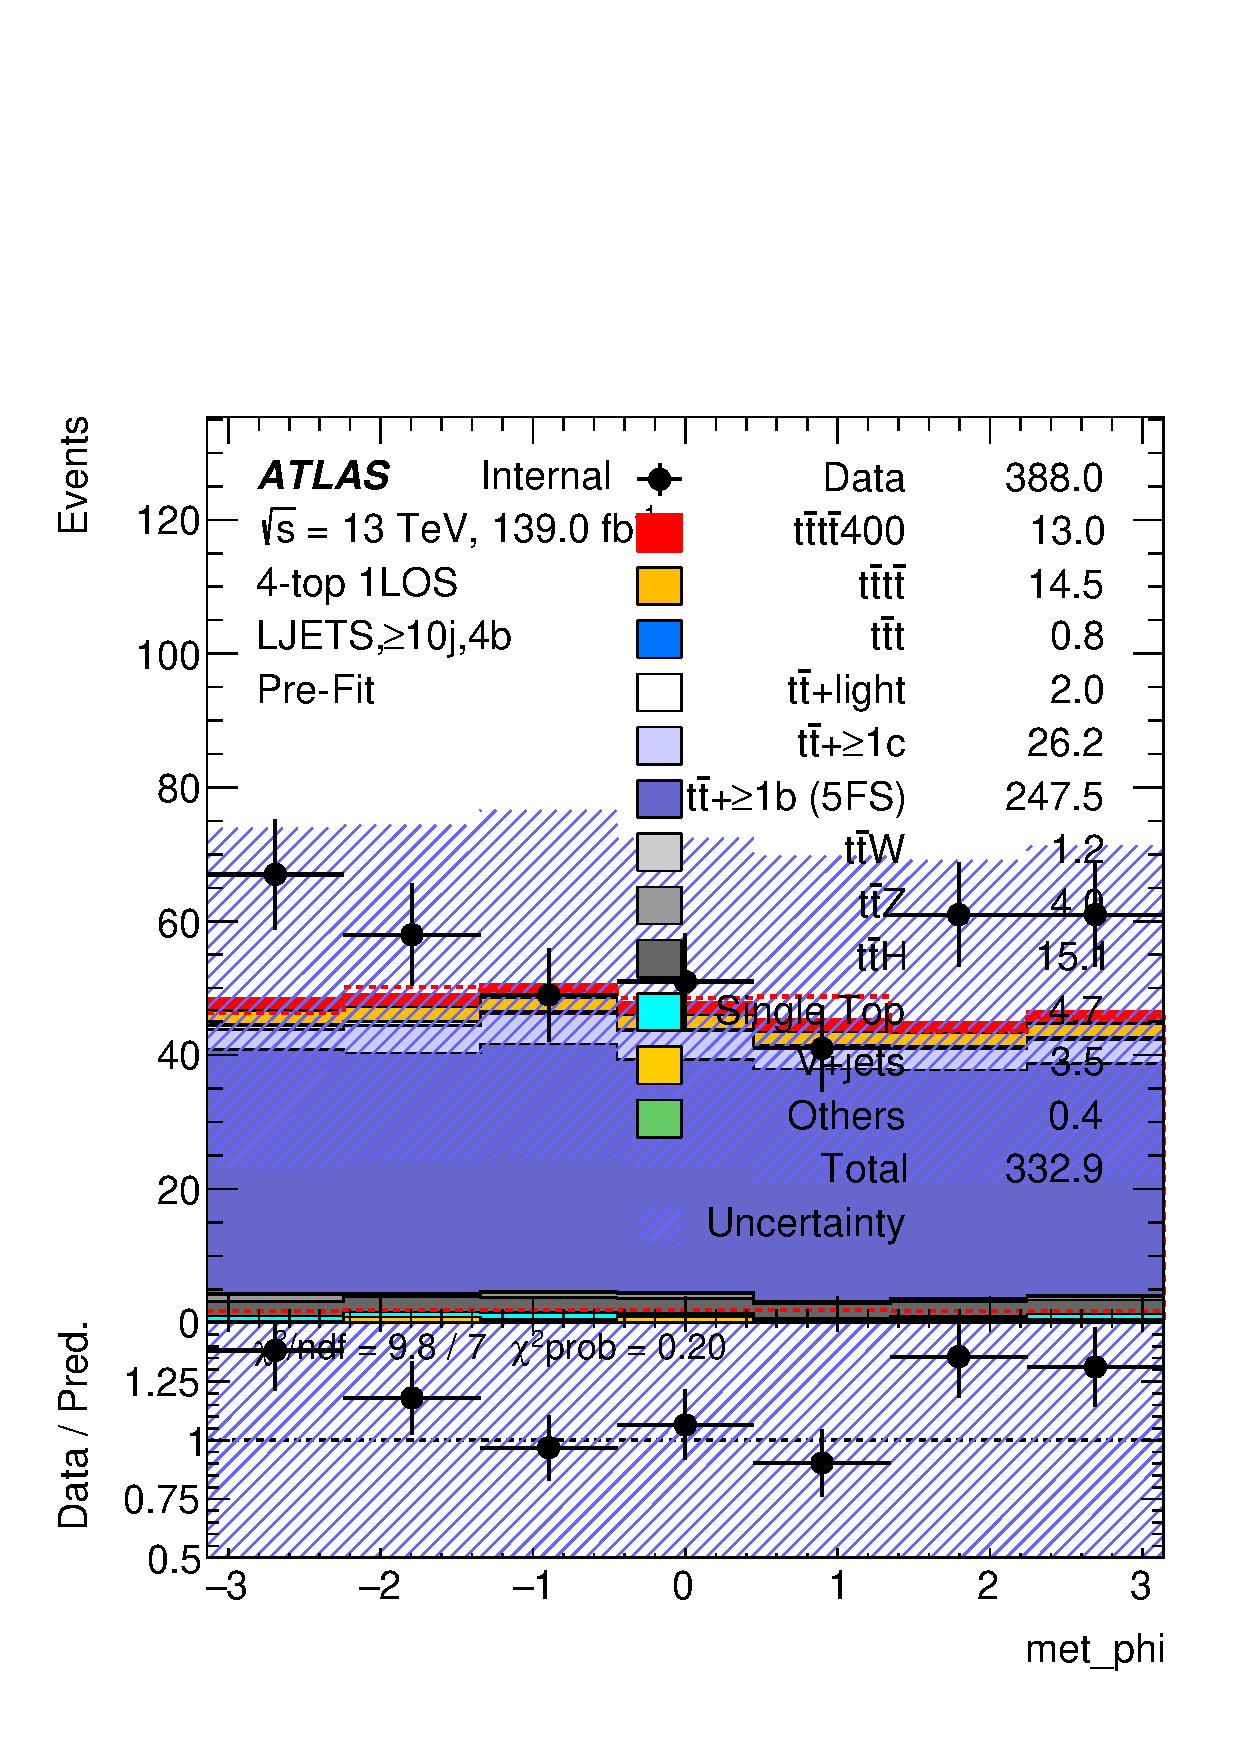
\includegraphics[width=0.23 \textwidth]{figures/fits/GNN/400/all/data_unblindedBonly/Plots/val_ljets_ge10j4b_met_phi.pdf} &
        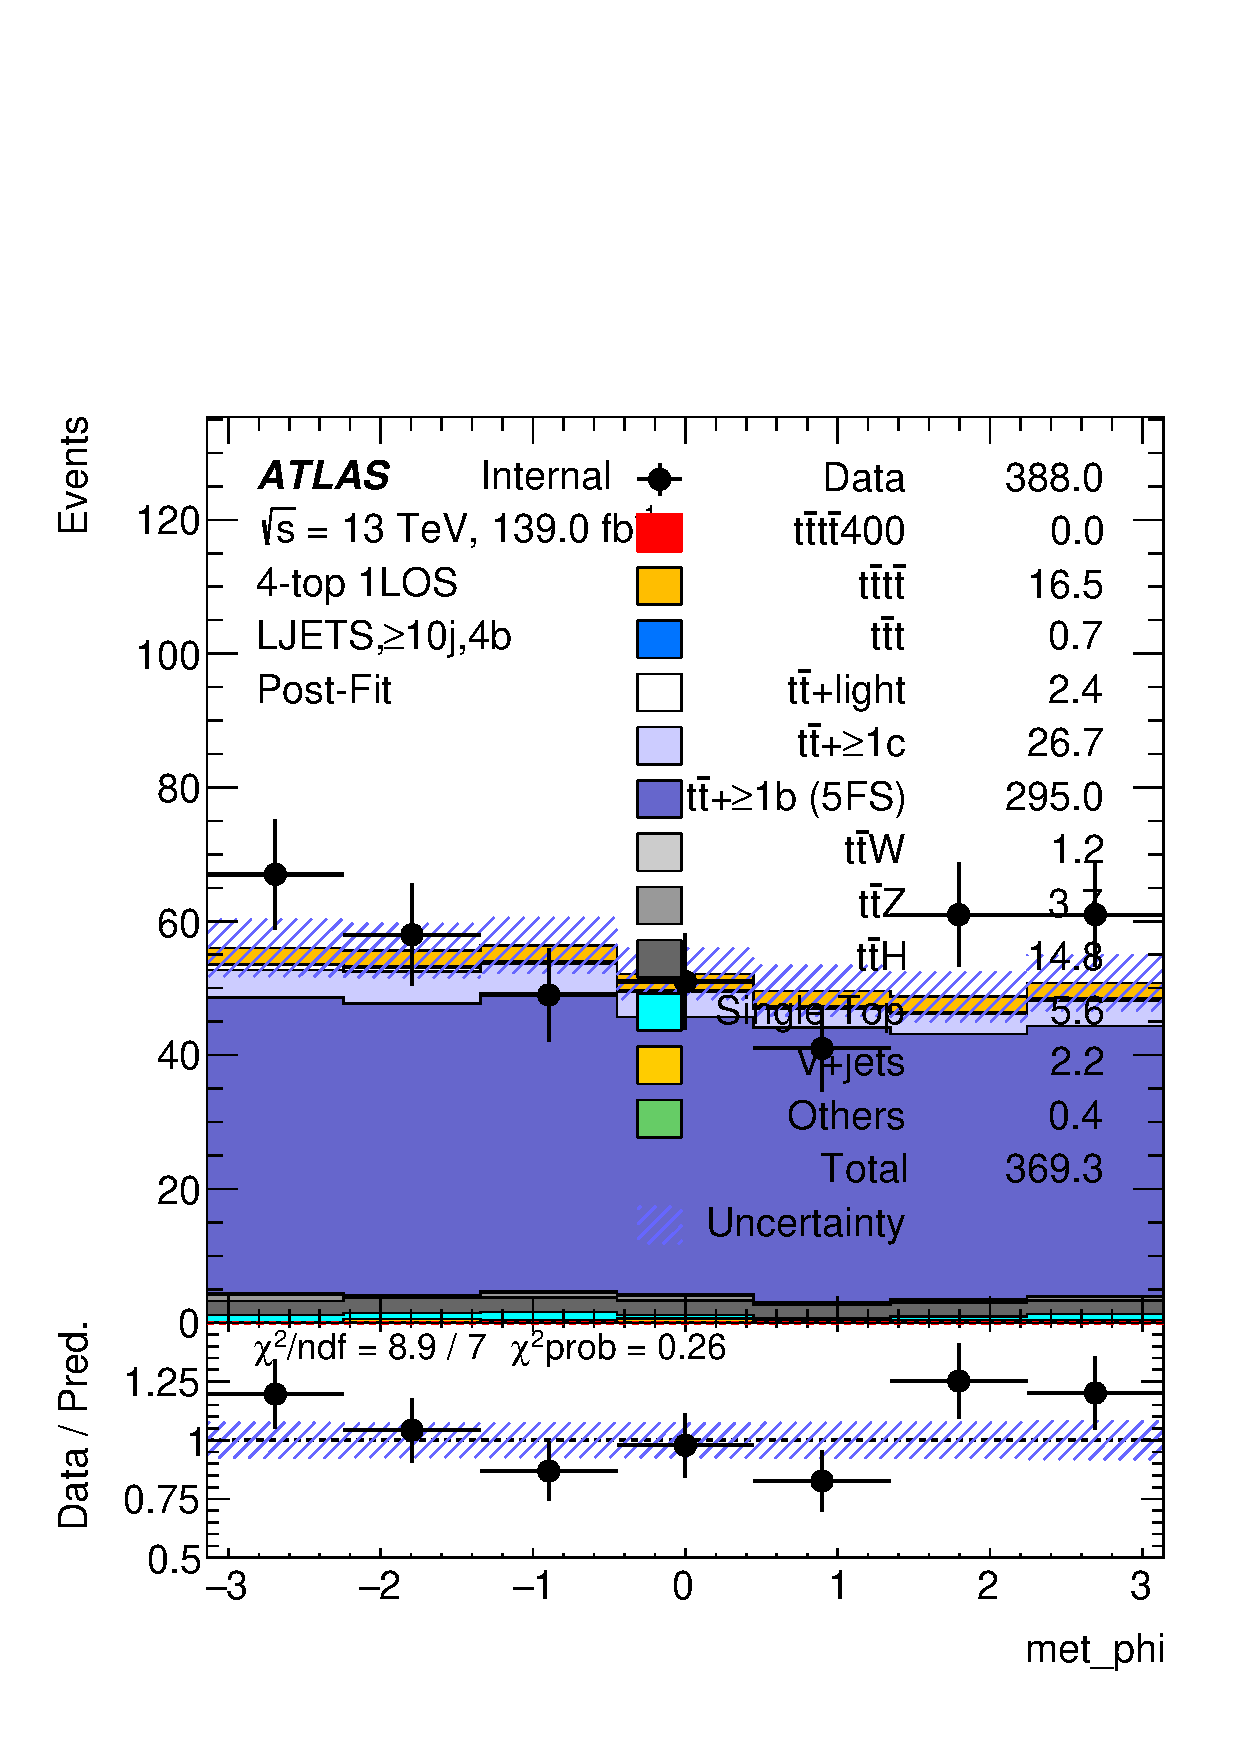
\includegraphics[width=0.23 \textwidth]{figures/fits/GNN/400/all/data_unblindedBonly/Plots/val_ljets_ge10j4b_met_phi_postFit.pdf} \\

        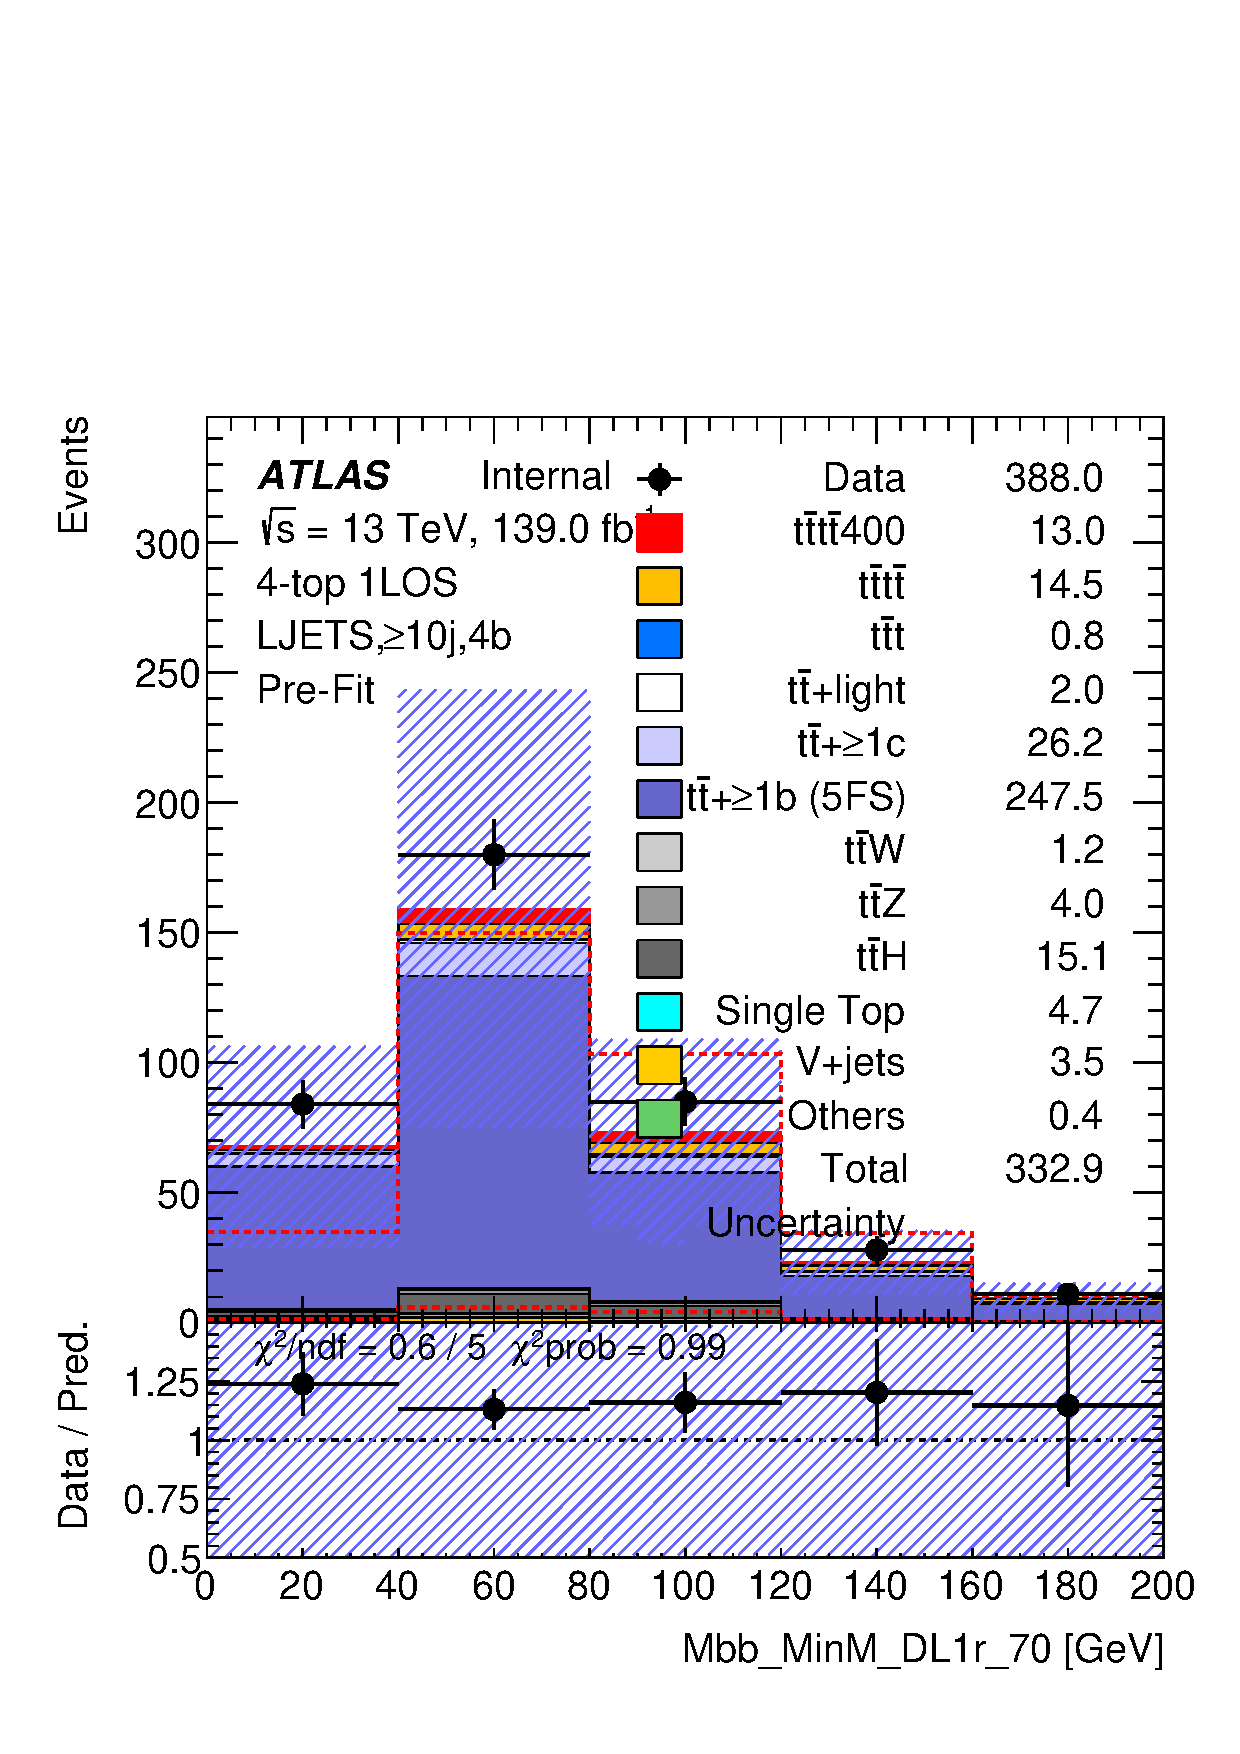
\includegraphics[width=0.23 \textwidth]{figures/fits/GNN/400/all/data_unblindedBonly/Plots/val_ljets_ge10j4b_Mbb_MinM_DL1r_70.pdf} &
        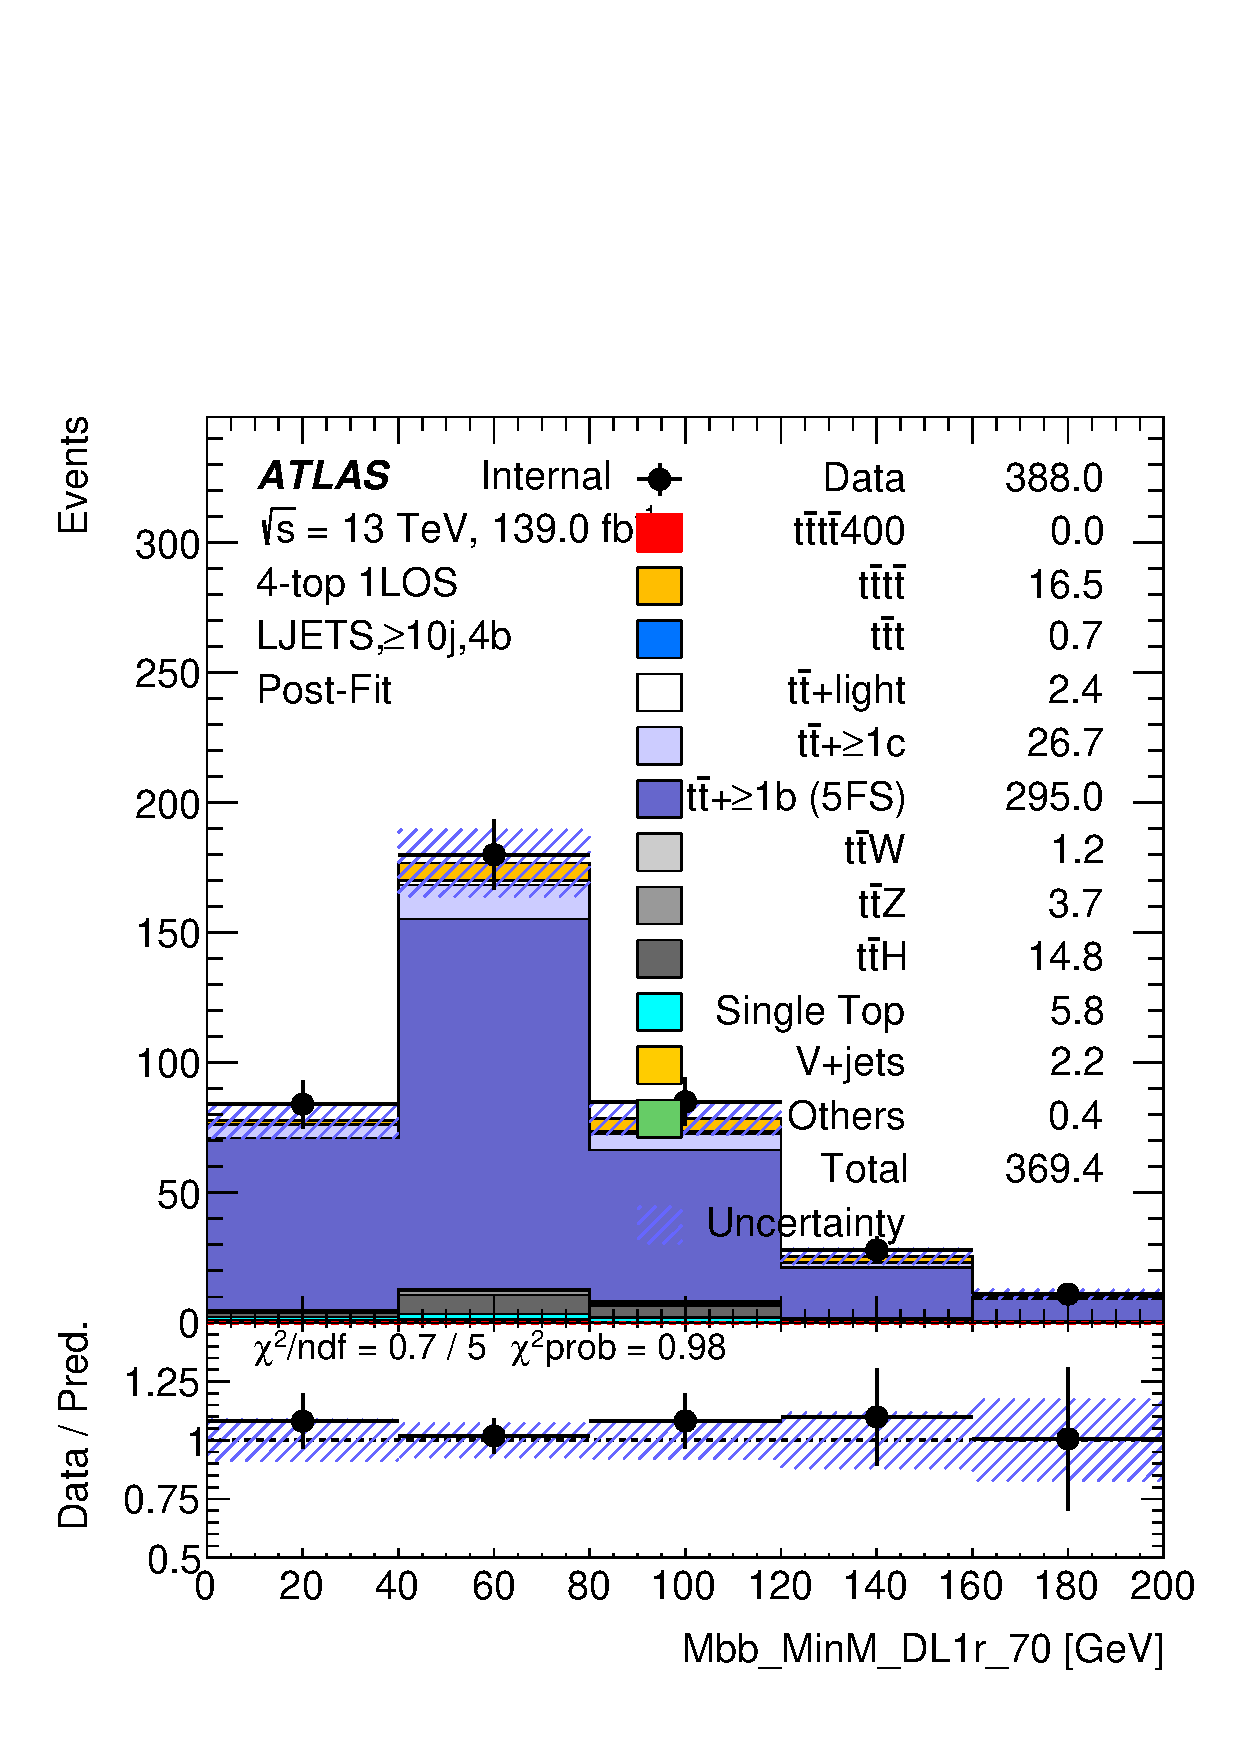
\includegraphics[width=0.23 \textwidth]{figures/fits/GNN/400/all/data_unblindedBonly/Plots/val_ljets_ge10j4b_Mbb_MinM_DL1r_70_postFit.pdf} &
        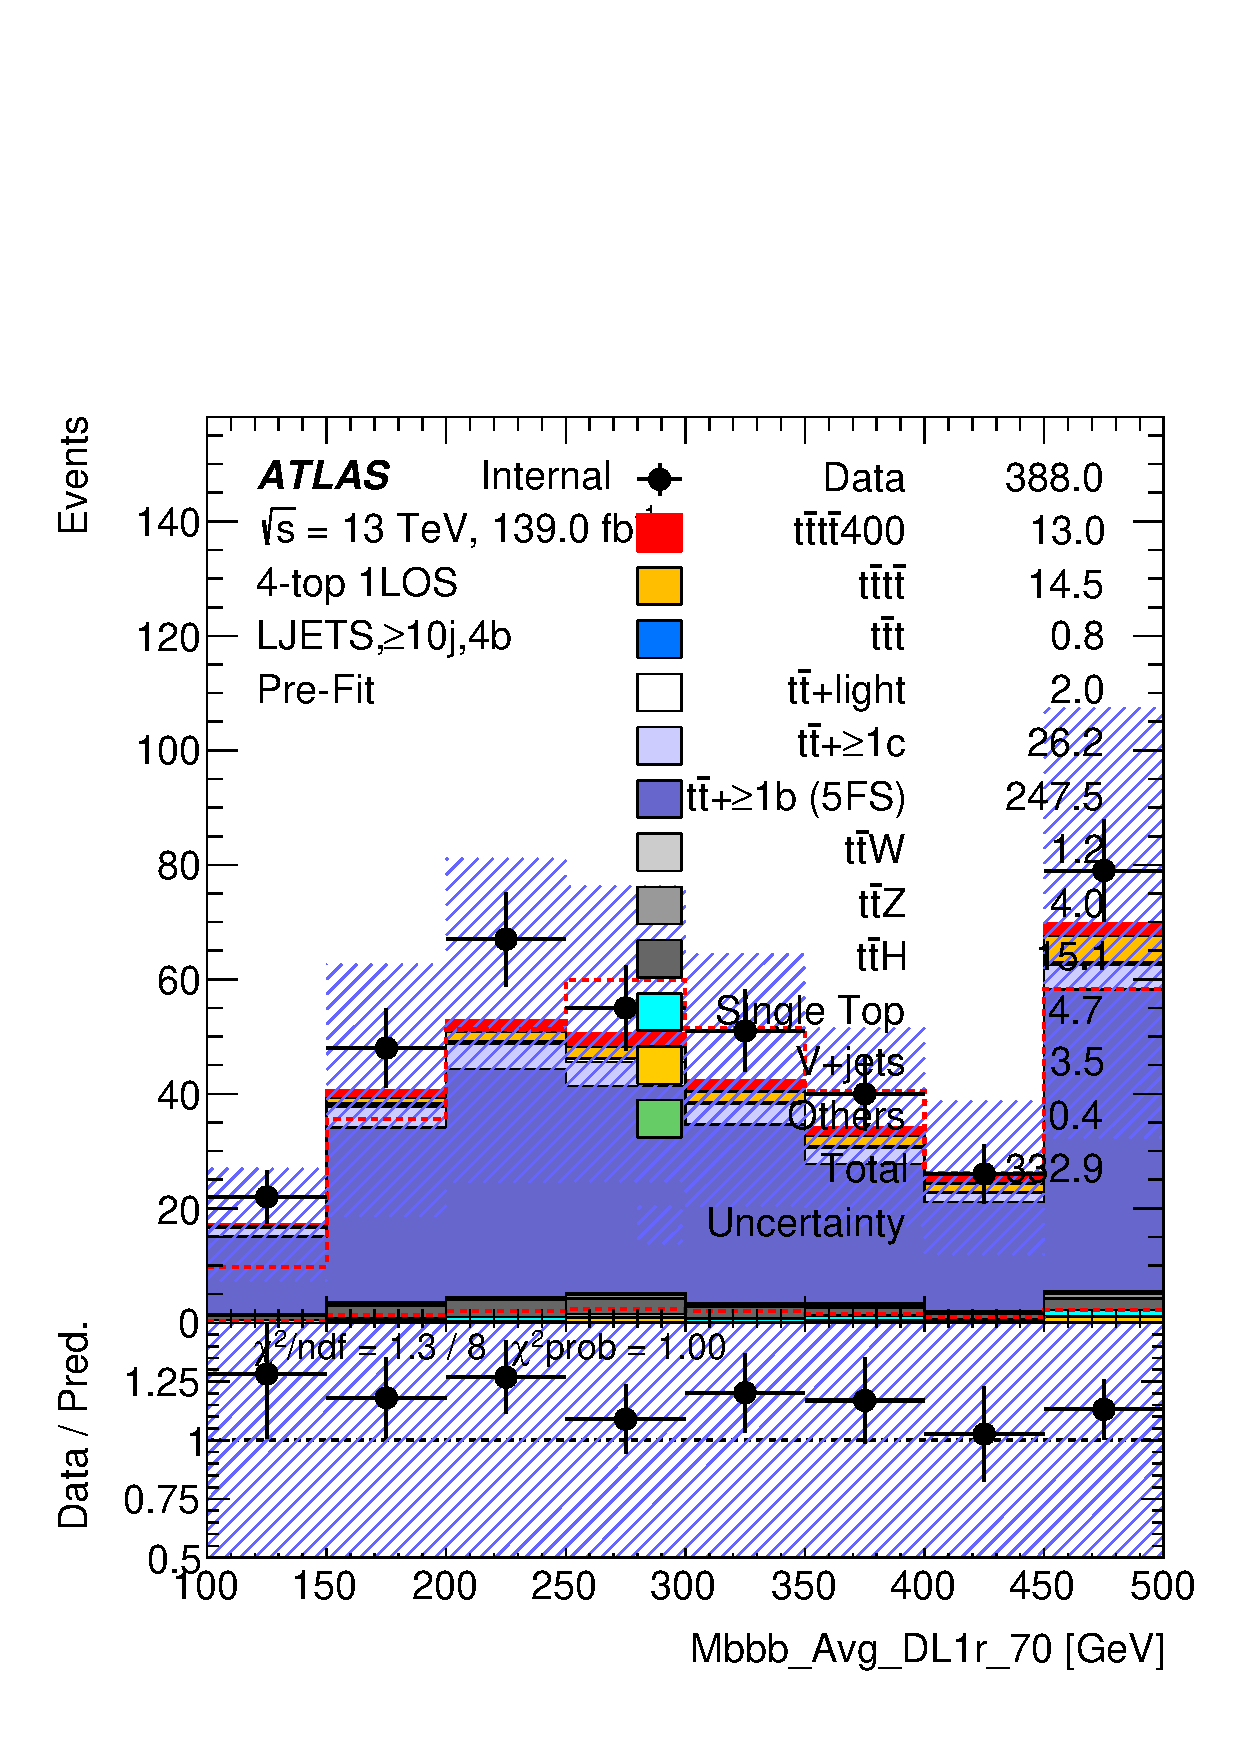
\includegraphics[width=0.23 \textwidth]{figures/fits/GNN/400/all/data_unblindedBonly/Plots/val_ljets_ge10j4b_Mbbb_Avg_DL1r_70.pdf} &
        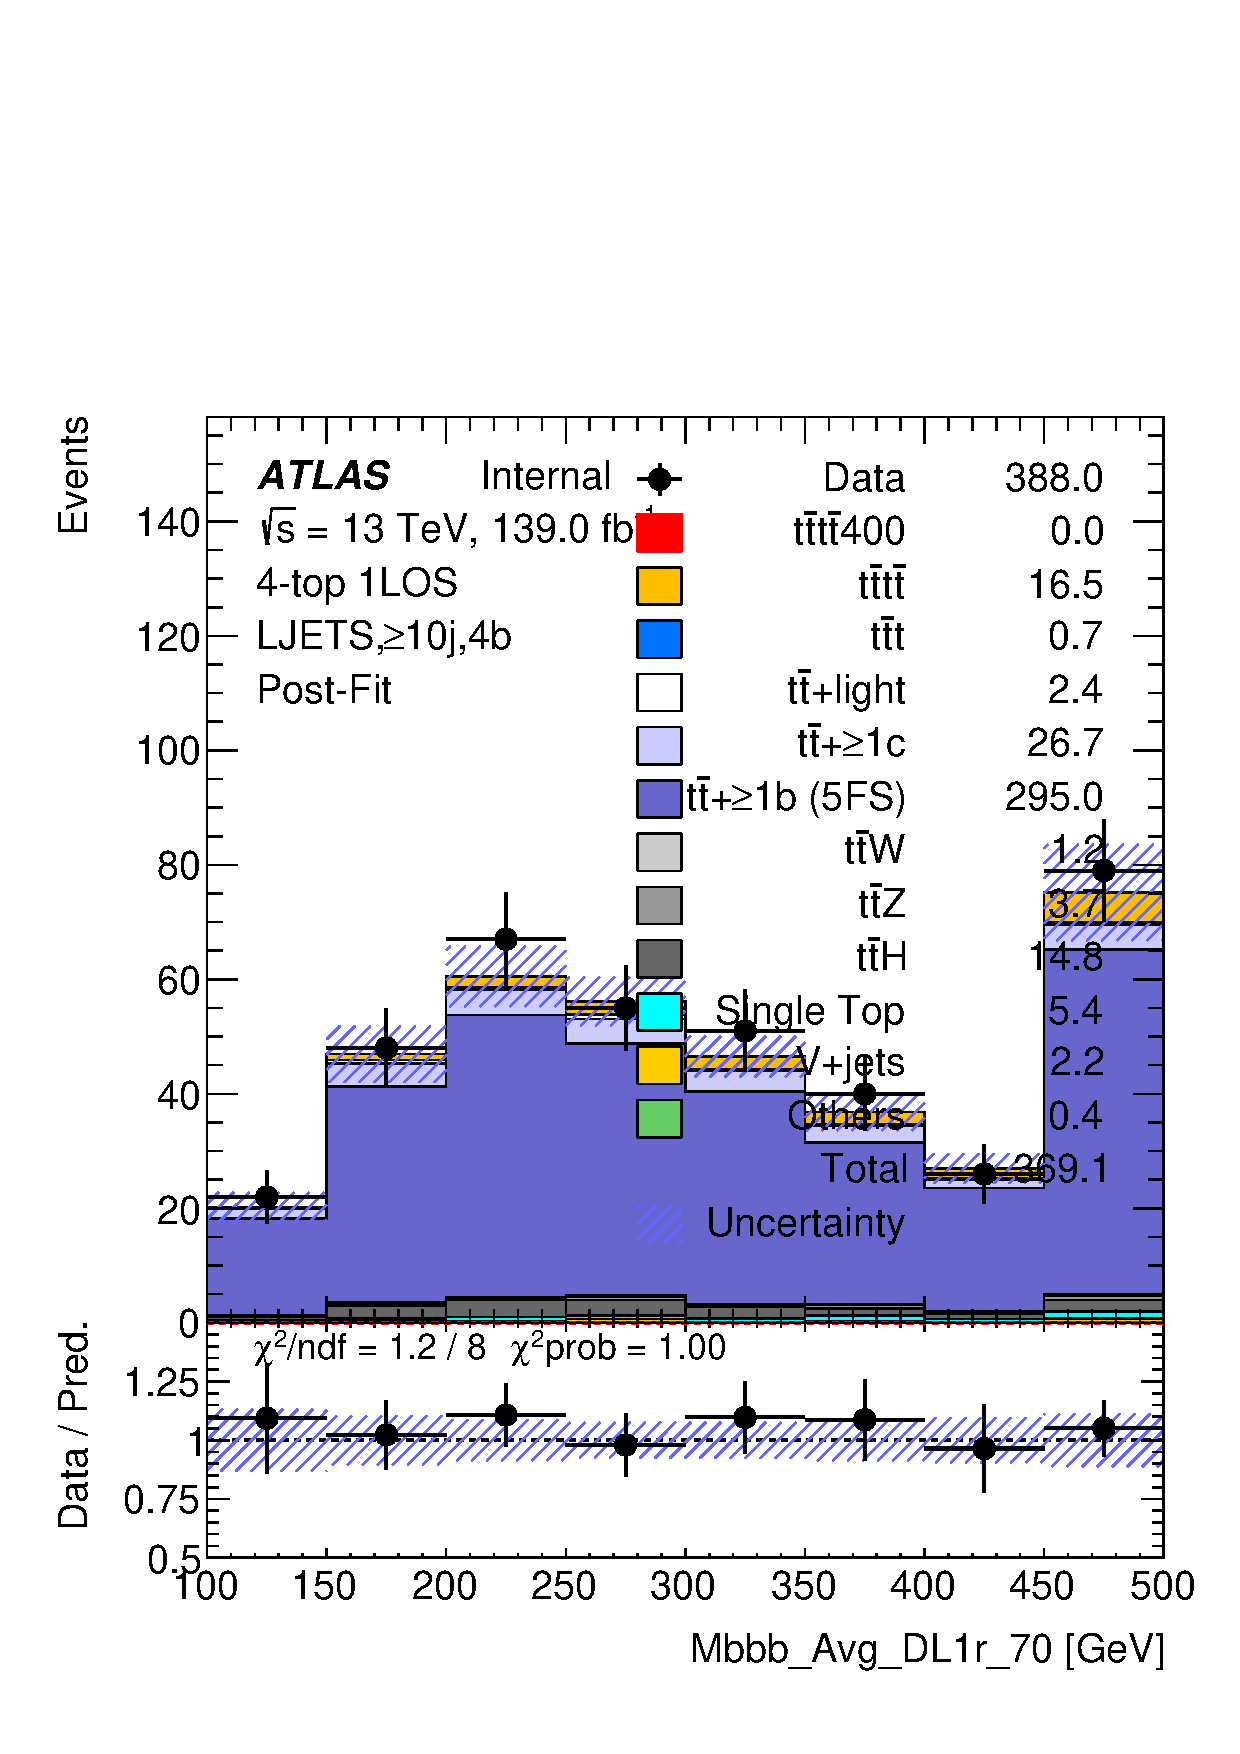
\includegraphics[width=0.23 \textwidth]{figures/fits/GNN/400/all/data_unblindedBonly/Plots/val_ljets_ge10j4b_Mbbb_Avg_DL1r_70_postFit.pdf} \\

        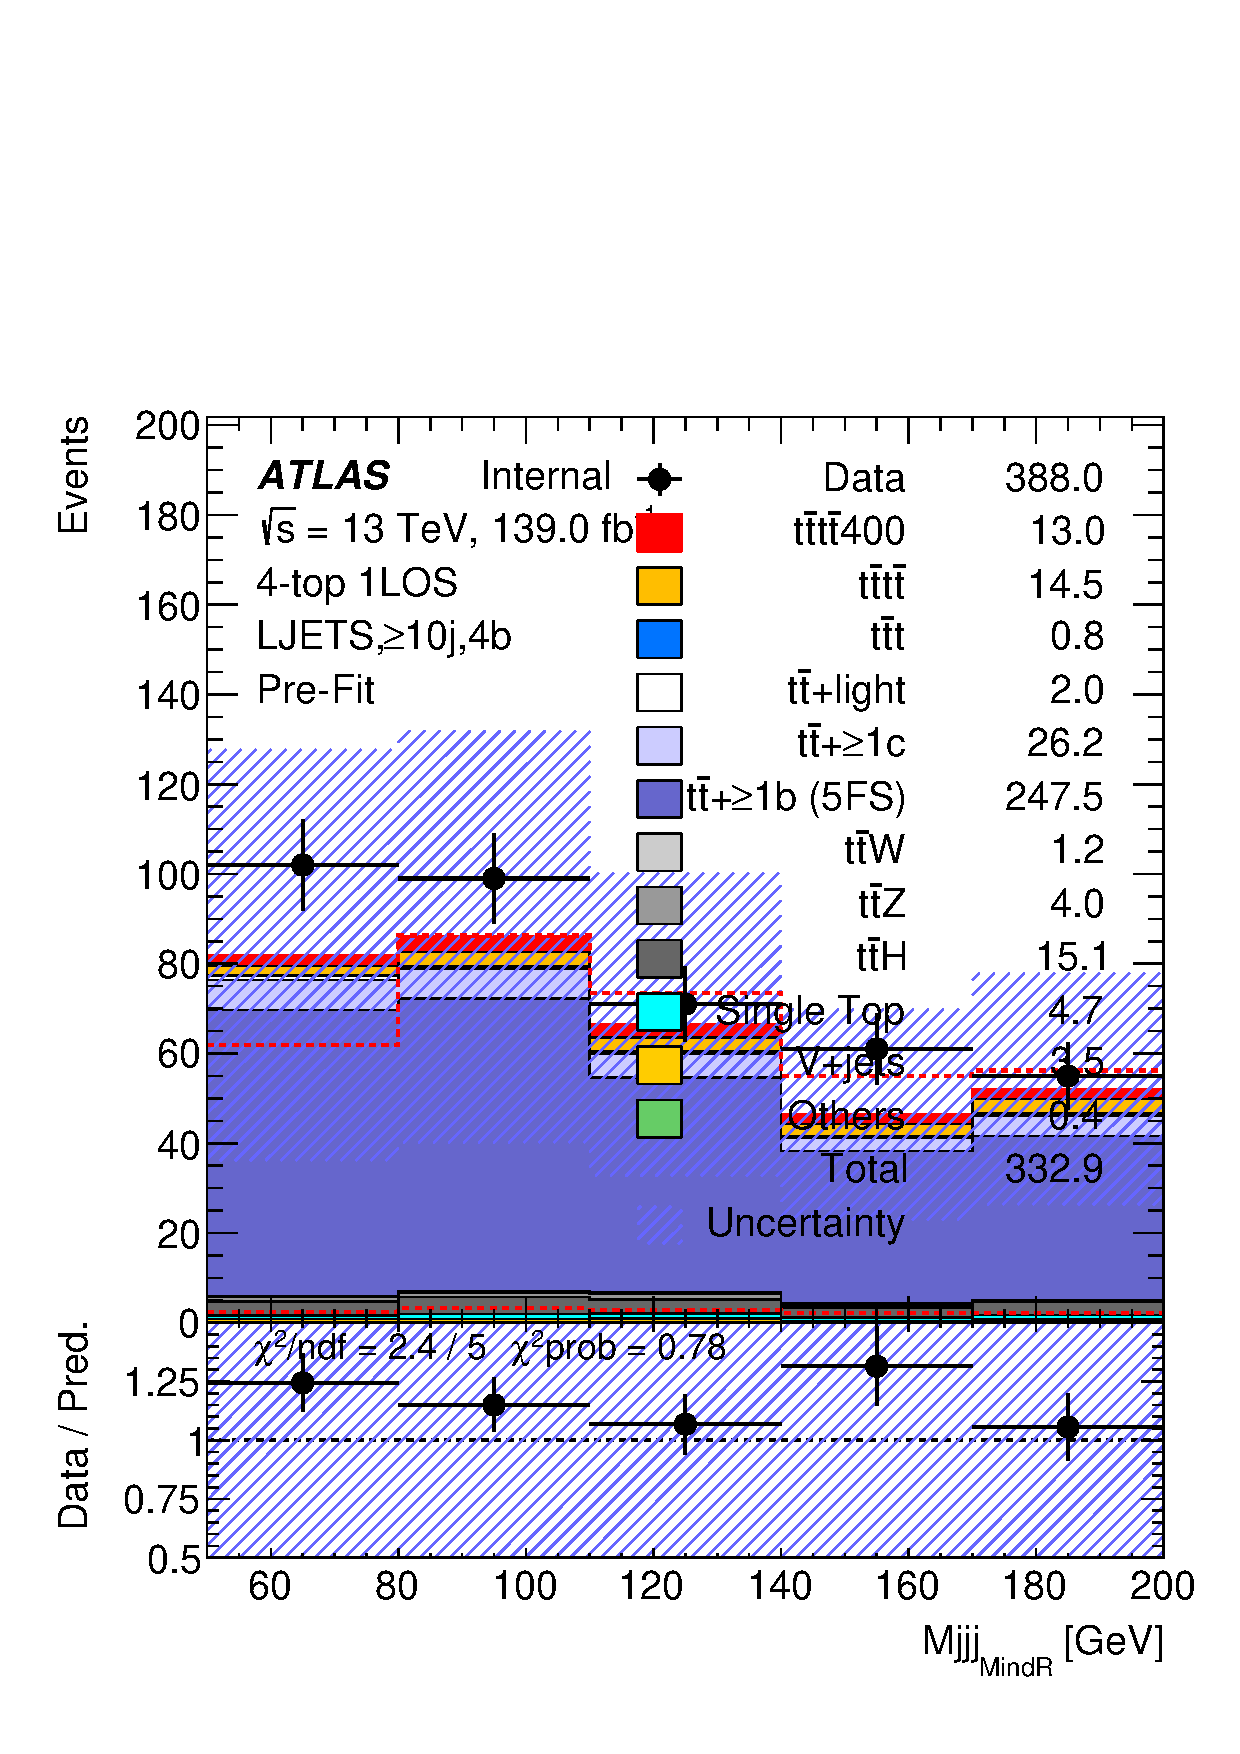
\includegraphics[width=0.23 \textwidth]{figures/fits/GNN/400/all/data_unblindedBonly/Plots/val_ljets_ge10j4b_Mjjj_MindR.pdf} &
        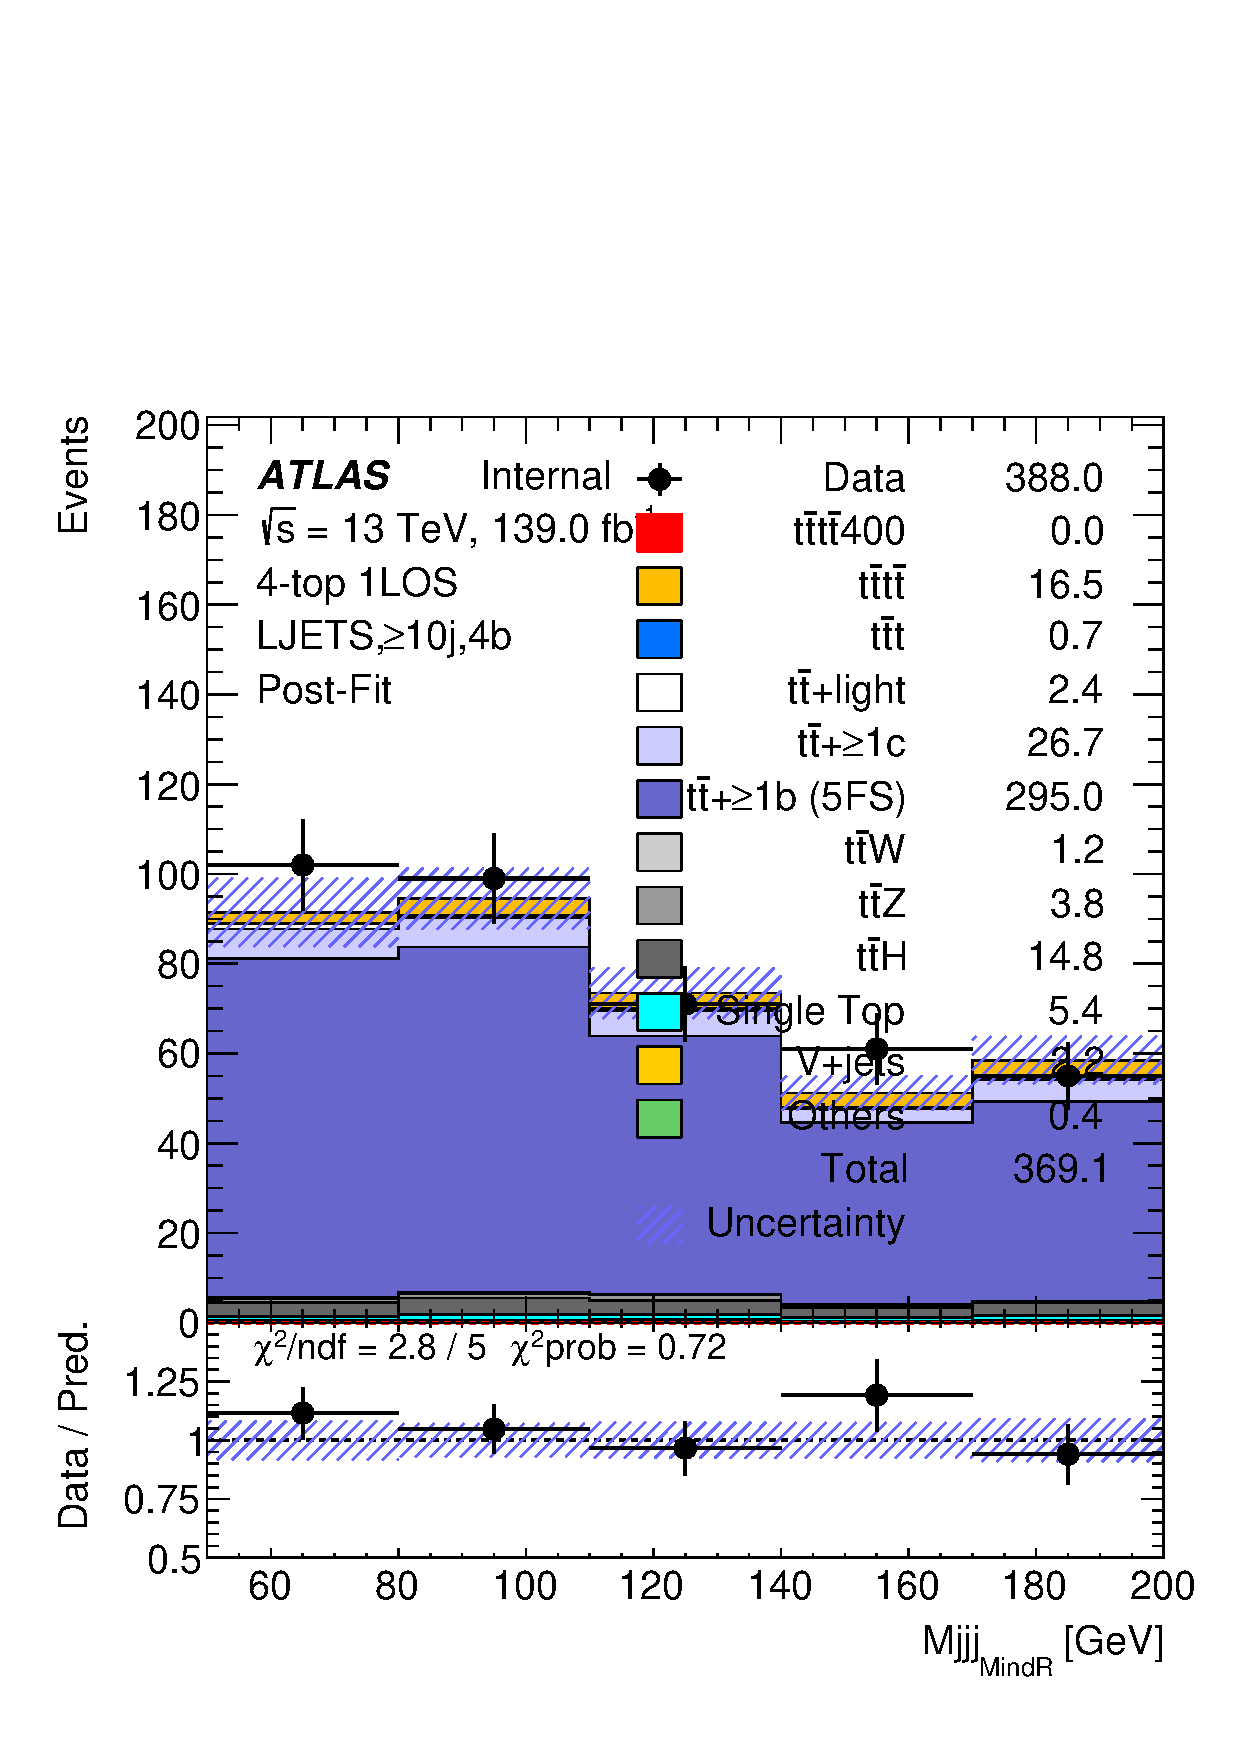
\includegraphics[width=0.23 \textwidth]{figures/fits/GNN/400/all/data_unblindedBonly/Plots/val_ljets_ge10j4b_Mjjj_MindR_postFit.pdf} &
        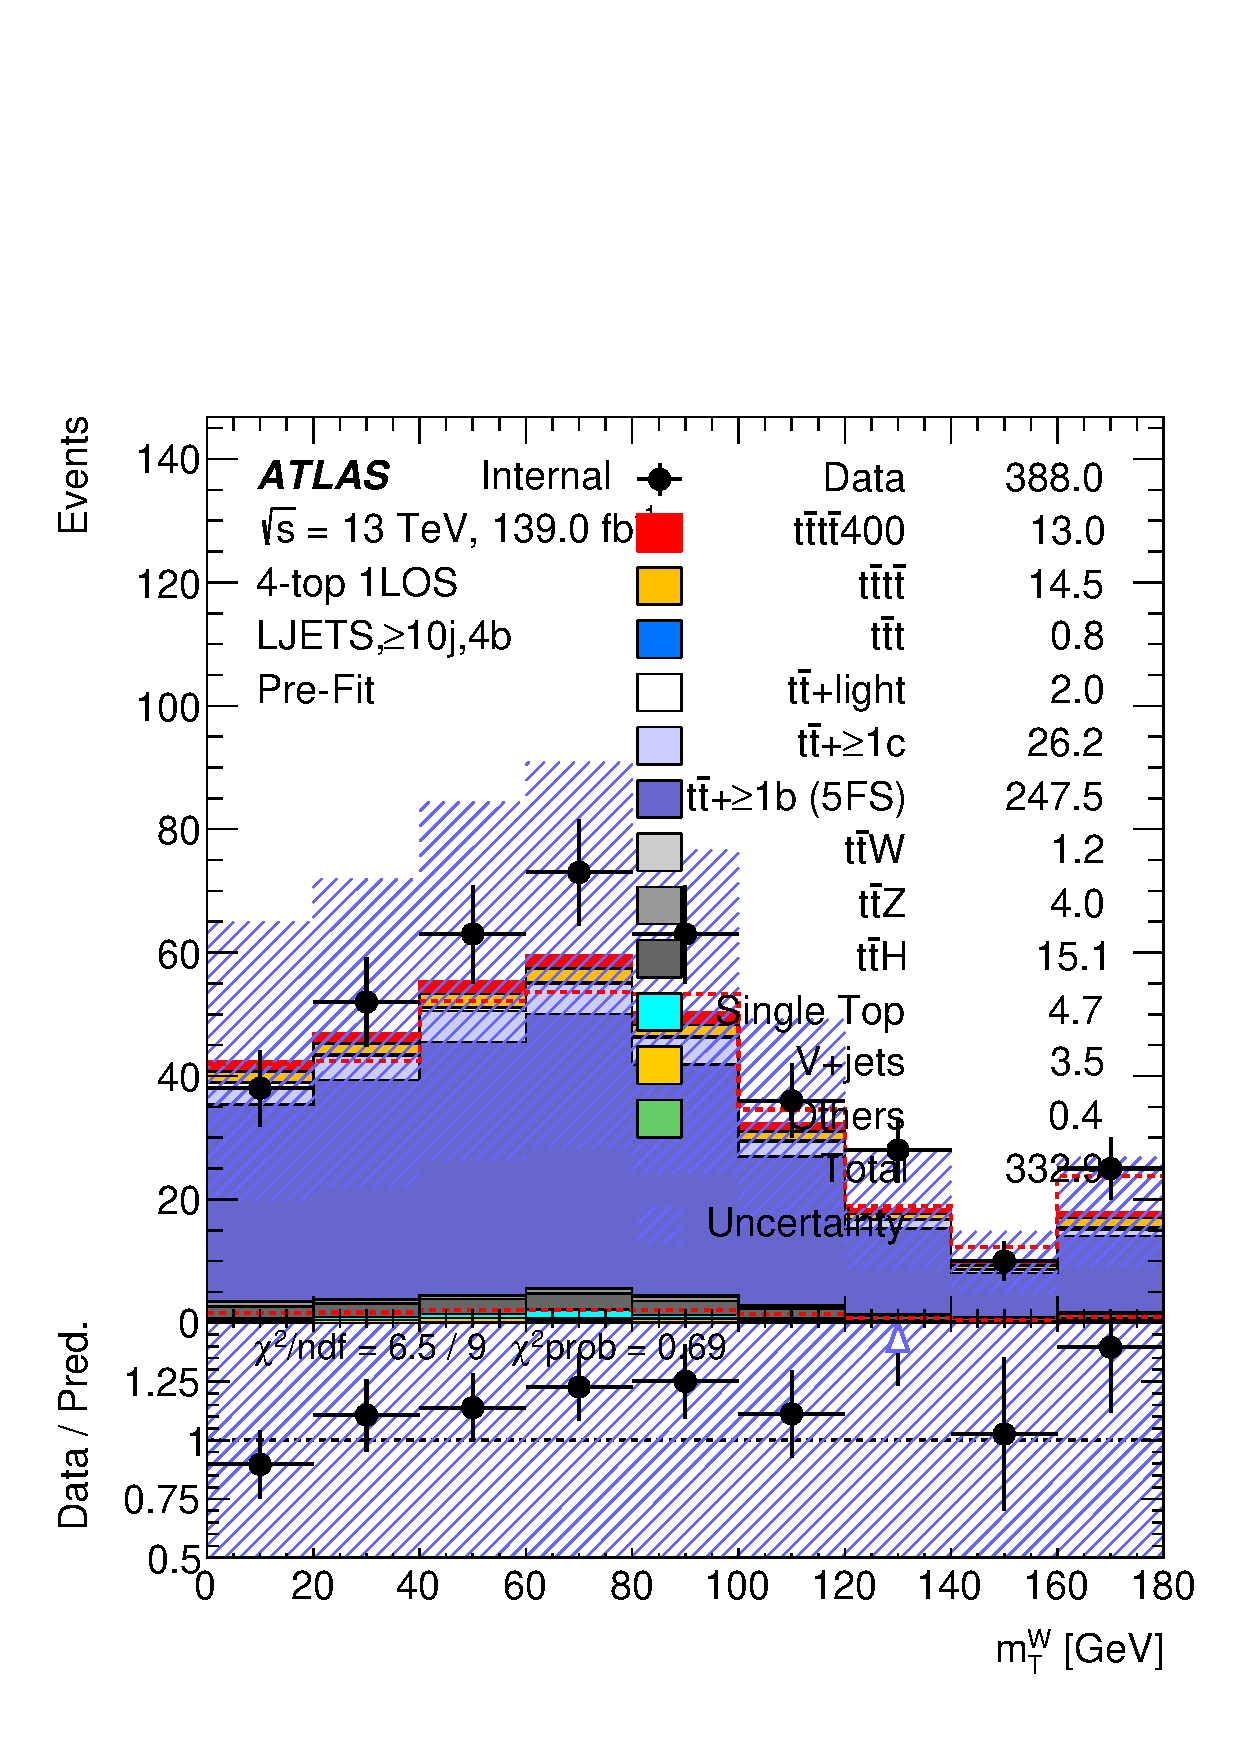
\includegraphics[width=0.23 \textwidth]{figures/fits/GNN/400/all/data_unblindedBonly/Plots/val_ljets_ge10j4b_mtw.pdf} &
        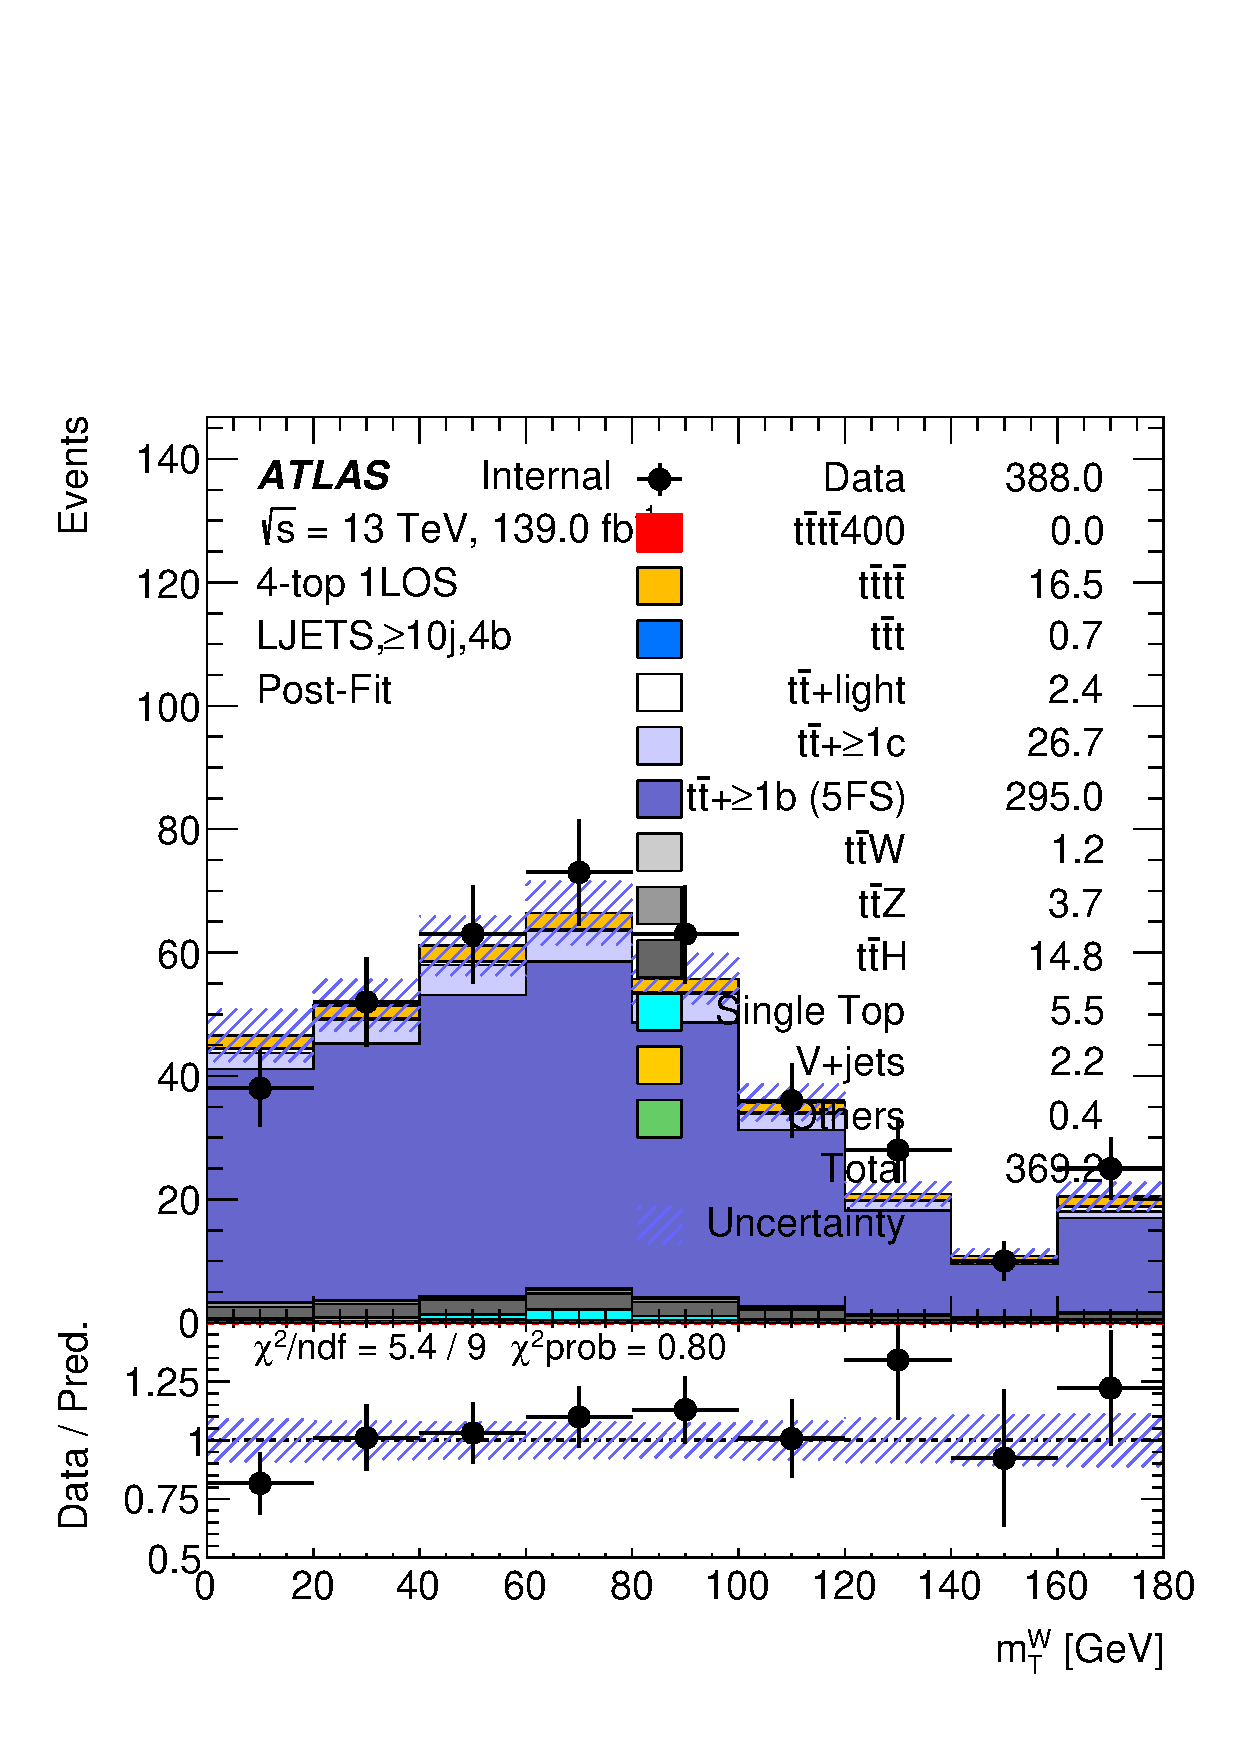
\includegraphics[width=0.23 \textwidth]{figures/fits/GNN/400/all/data_unblindedBonly/Plots/val_ljets_ge10j4b_mtw_postFit.pdf} \\

        \end{tabular}
        \end{center}

\caption{\label{GNN_input_val_2}Pre-fit(left) and Post-fit(right) distributions for GNN input variables in the ge10j4b region.}
\end{figure}

\begin{figure}

        \begin{center} \setlength{\tabcolsep}{2.5pt}\footnotesize
        \begin{tabular}{cccc}

        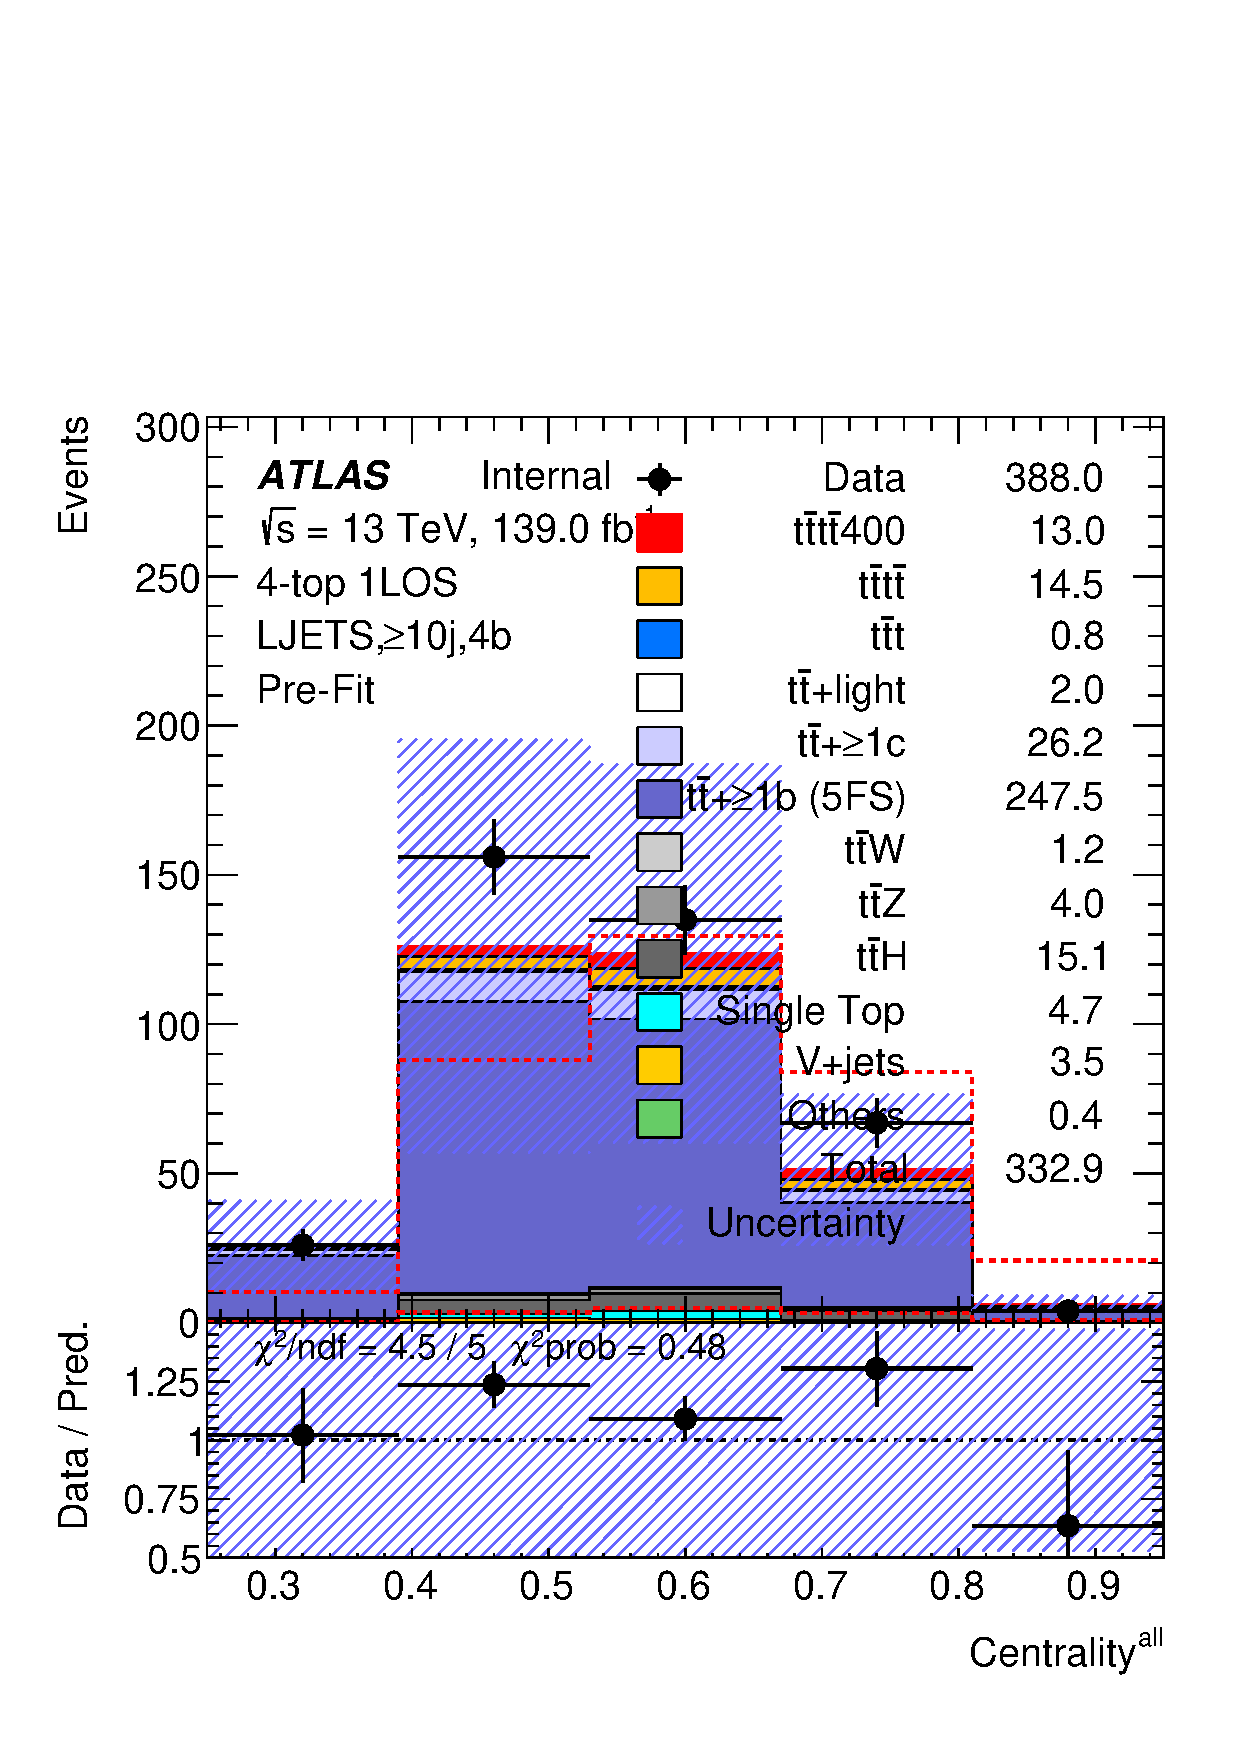
\includegraphics[width=0.23 \textwidth]{figures/fits/GNN/400/all/data_unblindedBonly/Plots/val_ljets_ge10j4b_centrality.pdf} &
        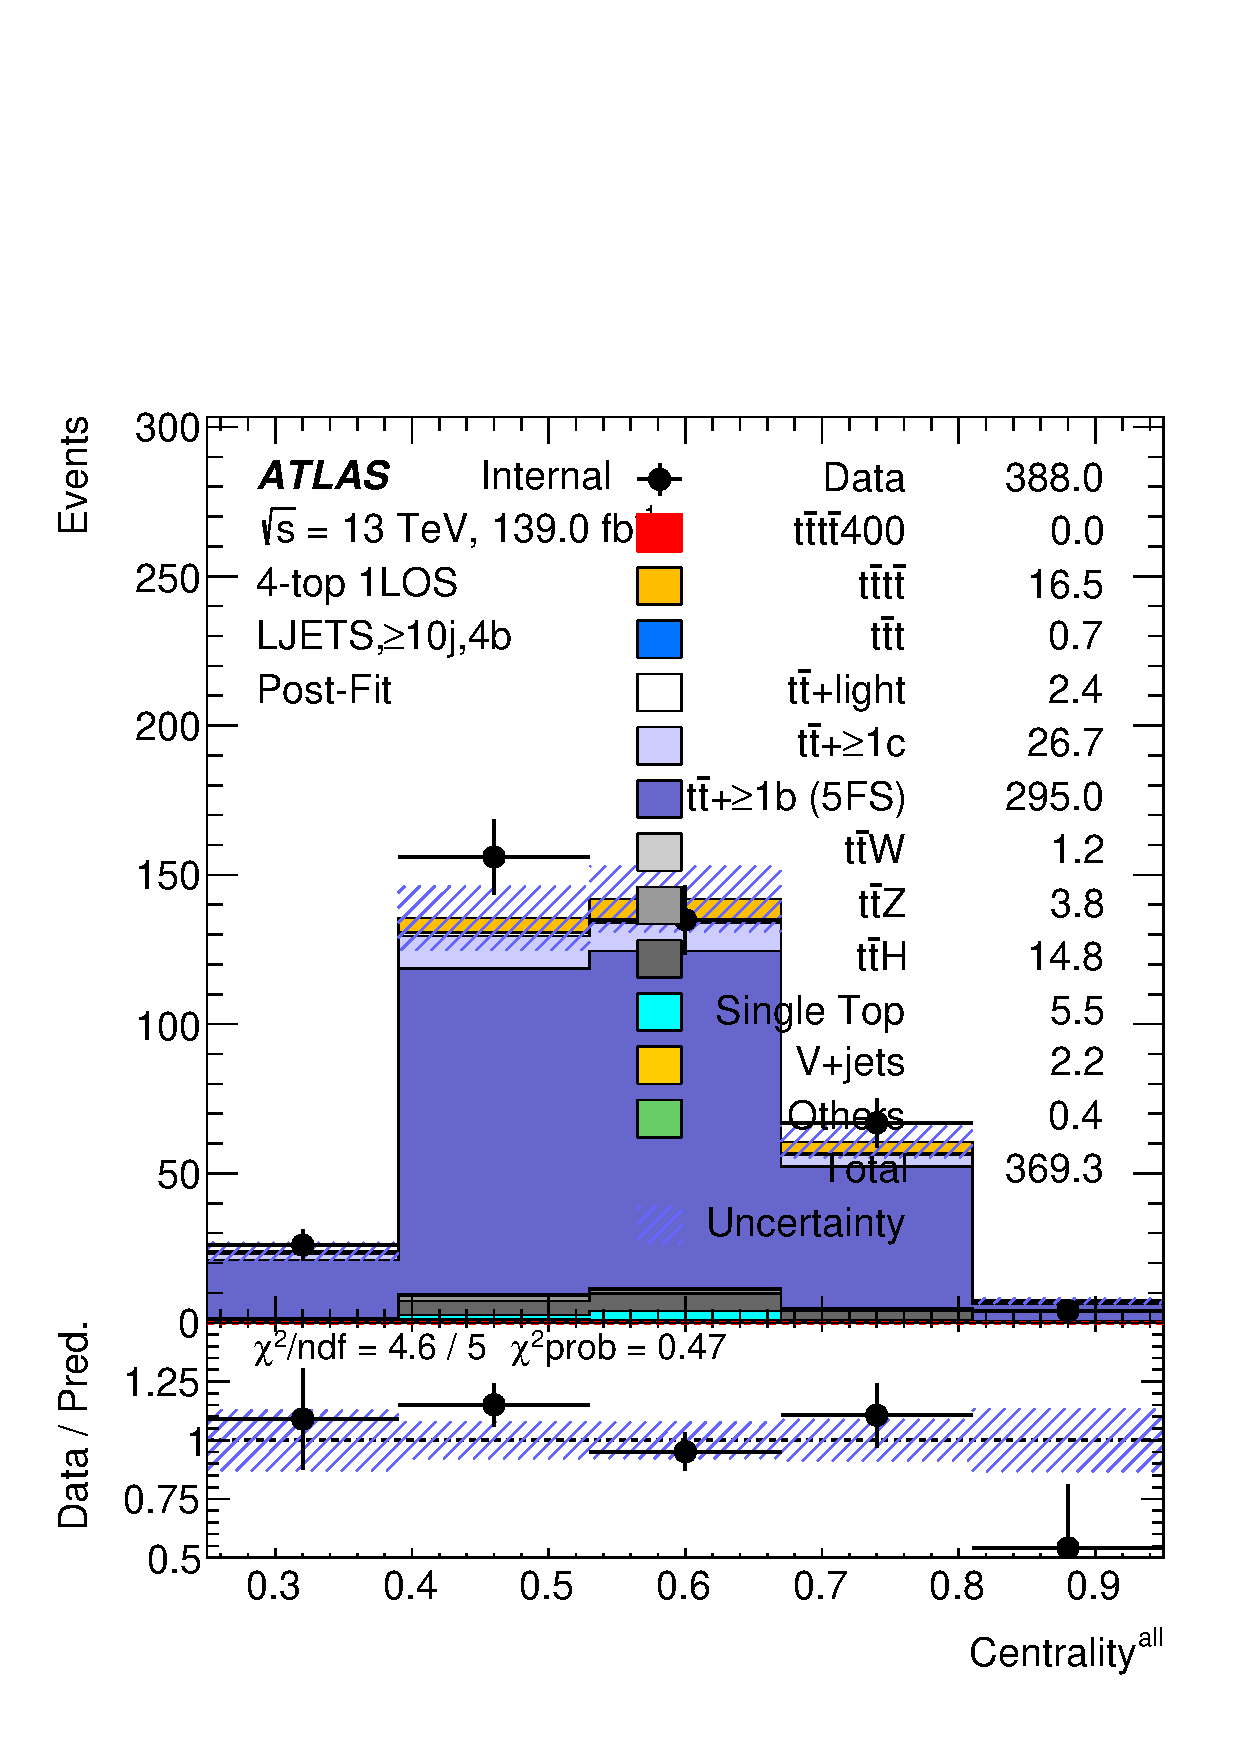
\includegraphics[width=0.23 \textwidth]{figures/fits/GNN/400/all/data_unblindedBonly/Plots/val_ljets_ge10j4b_centrality_postFit.pdf} &
        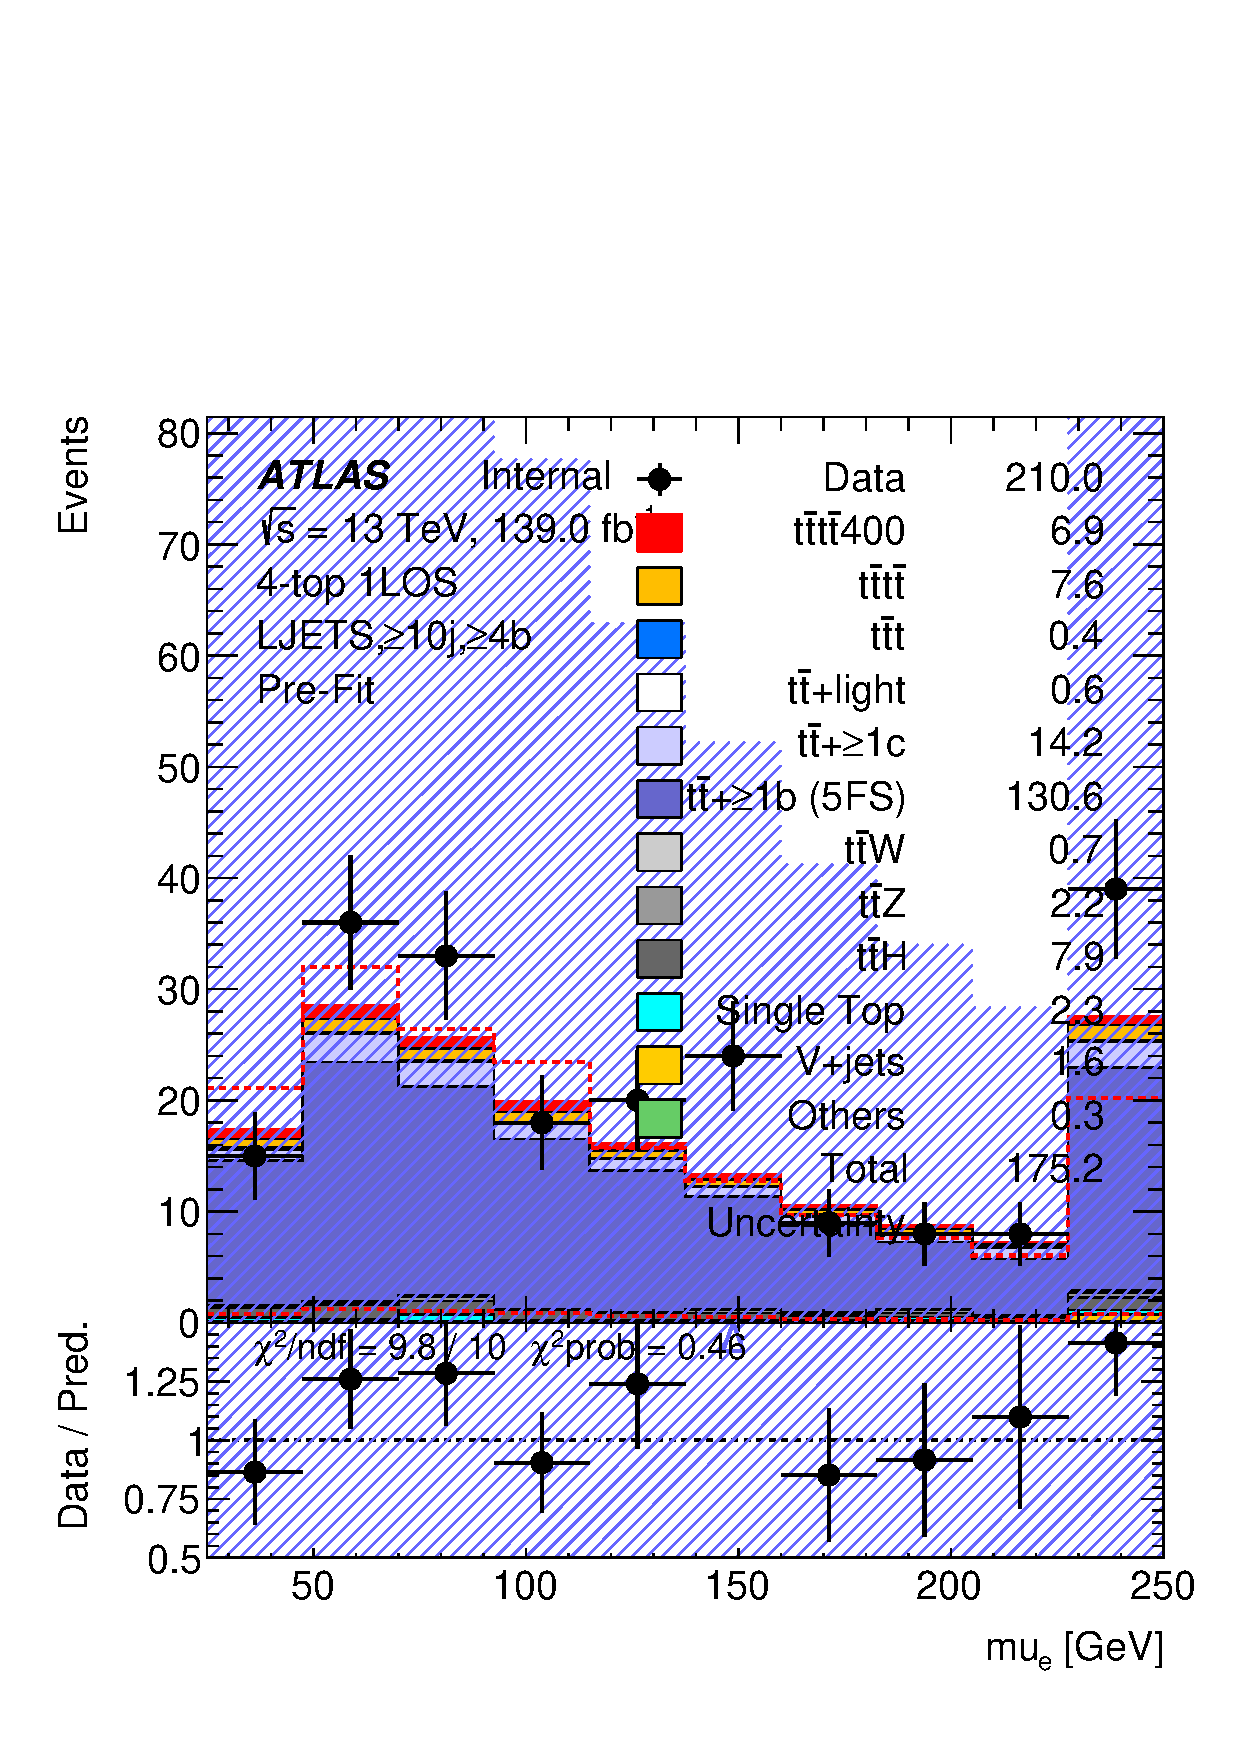
\includegraphics[width=0.23 \textwidth]{figures/fits/GNN/400/all/data_unblindedBonly/Plots/val_ljets_ge10j4b_mu_e.pdf} &
        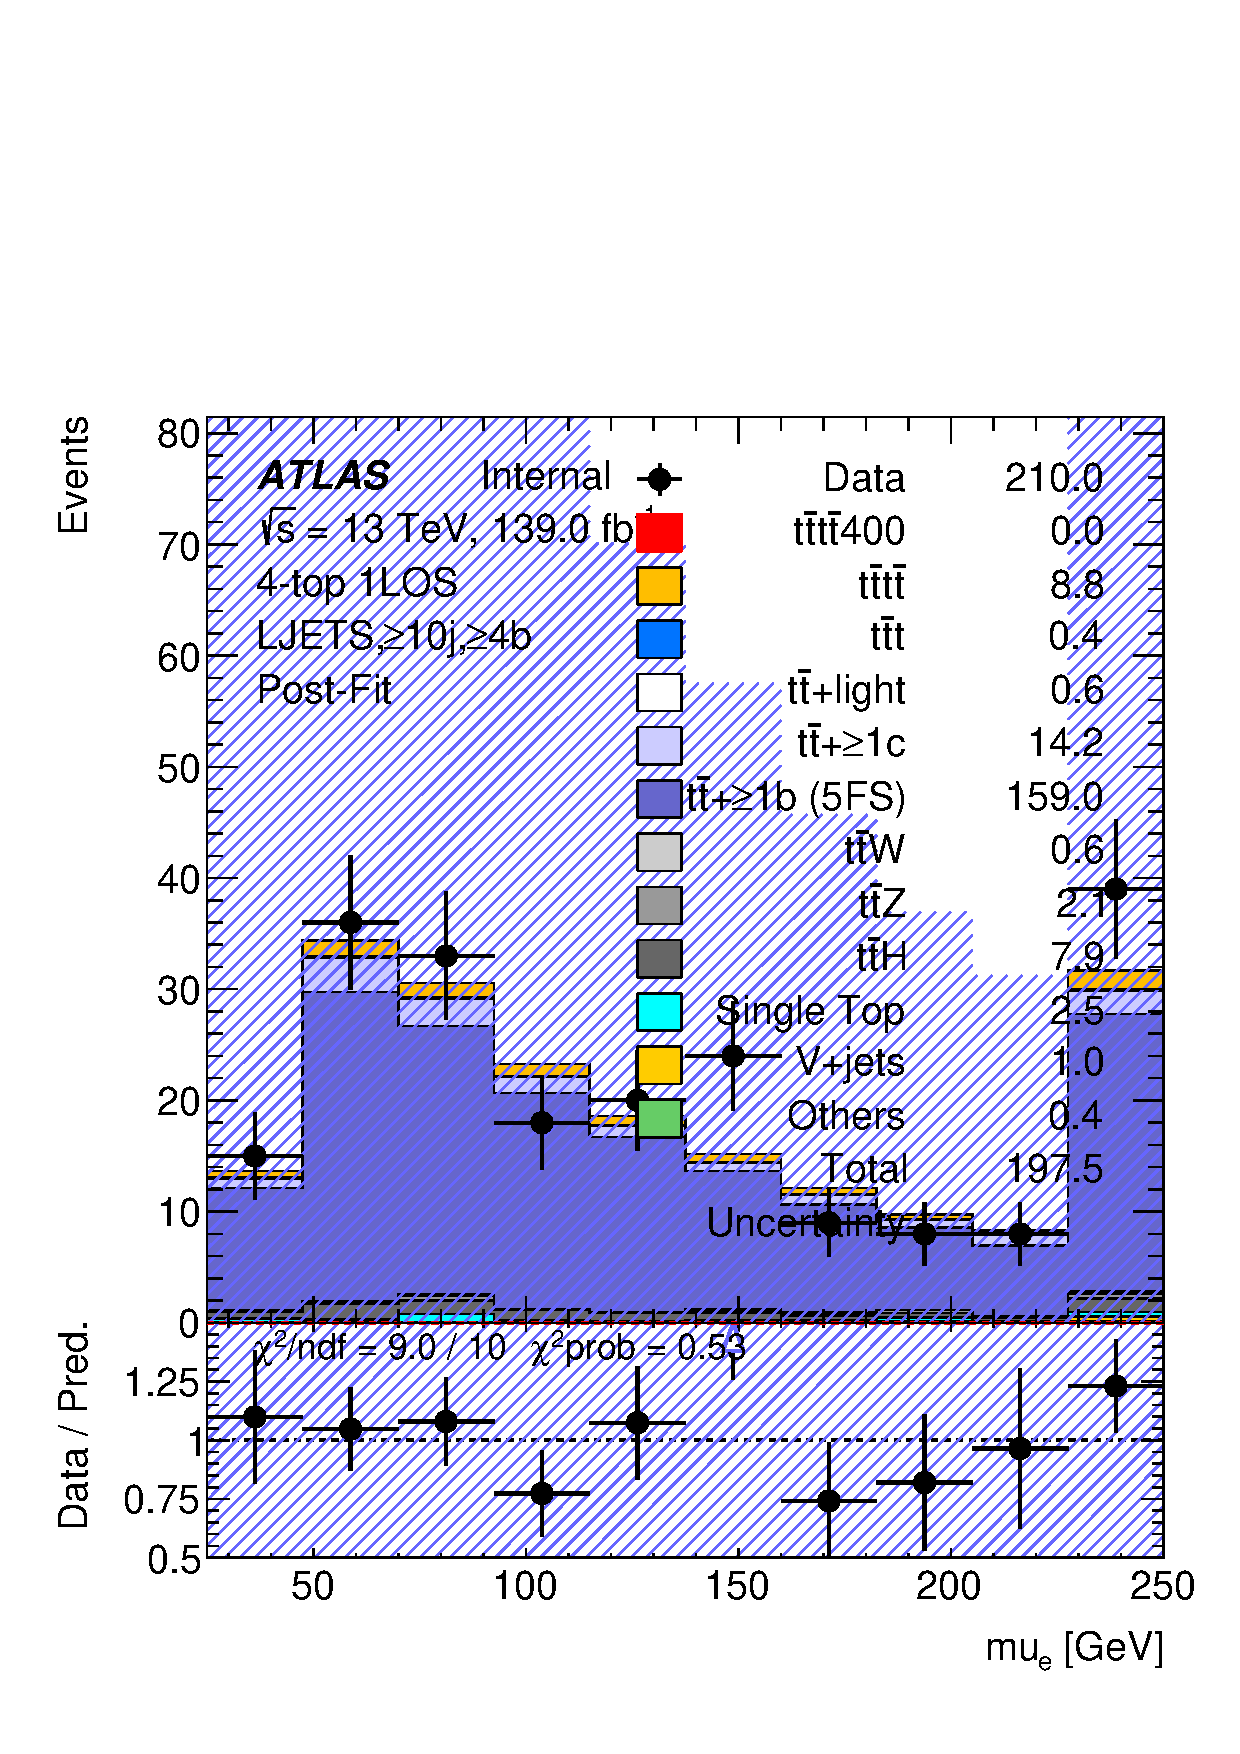
\includegraphics[width=0.23 \textwidth]{figures/fits/GNN/400/all/data_unblindedBonly/Plots/val_ljets_ge10j4b_mu_e_postFit.pdf} \\

        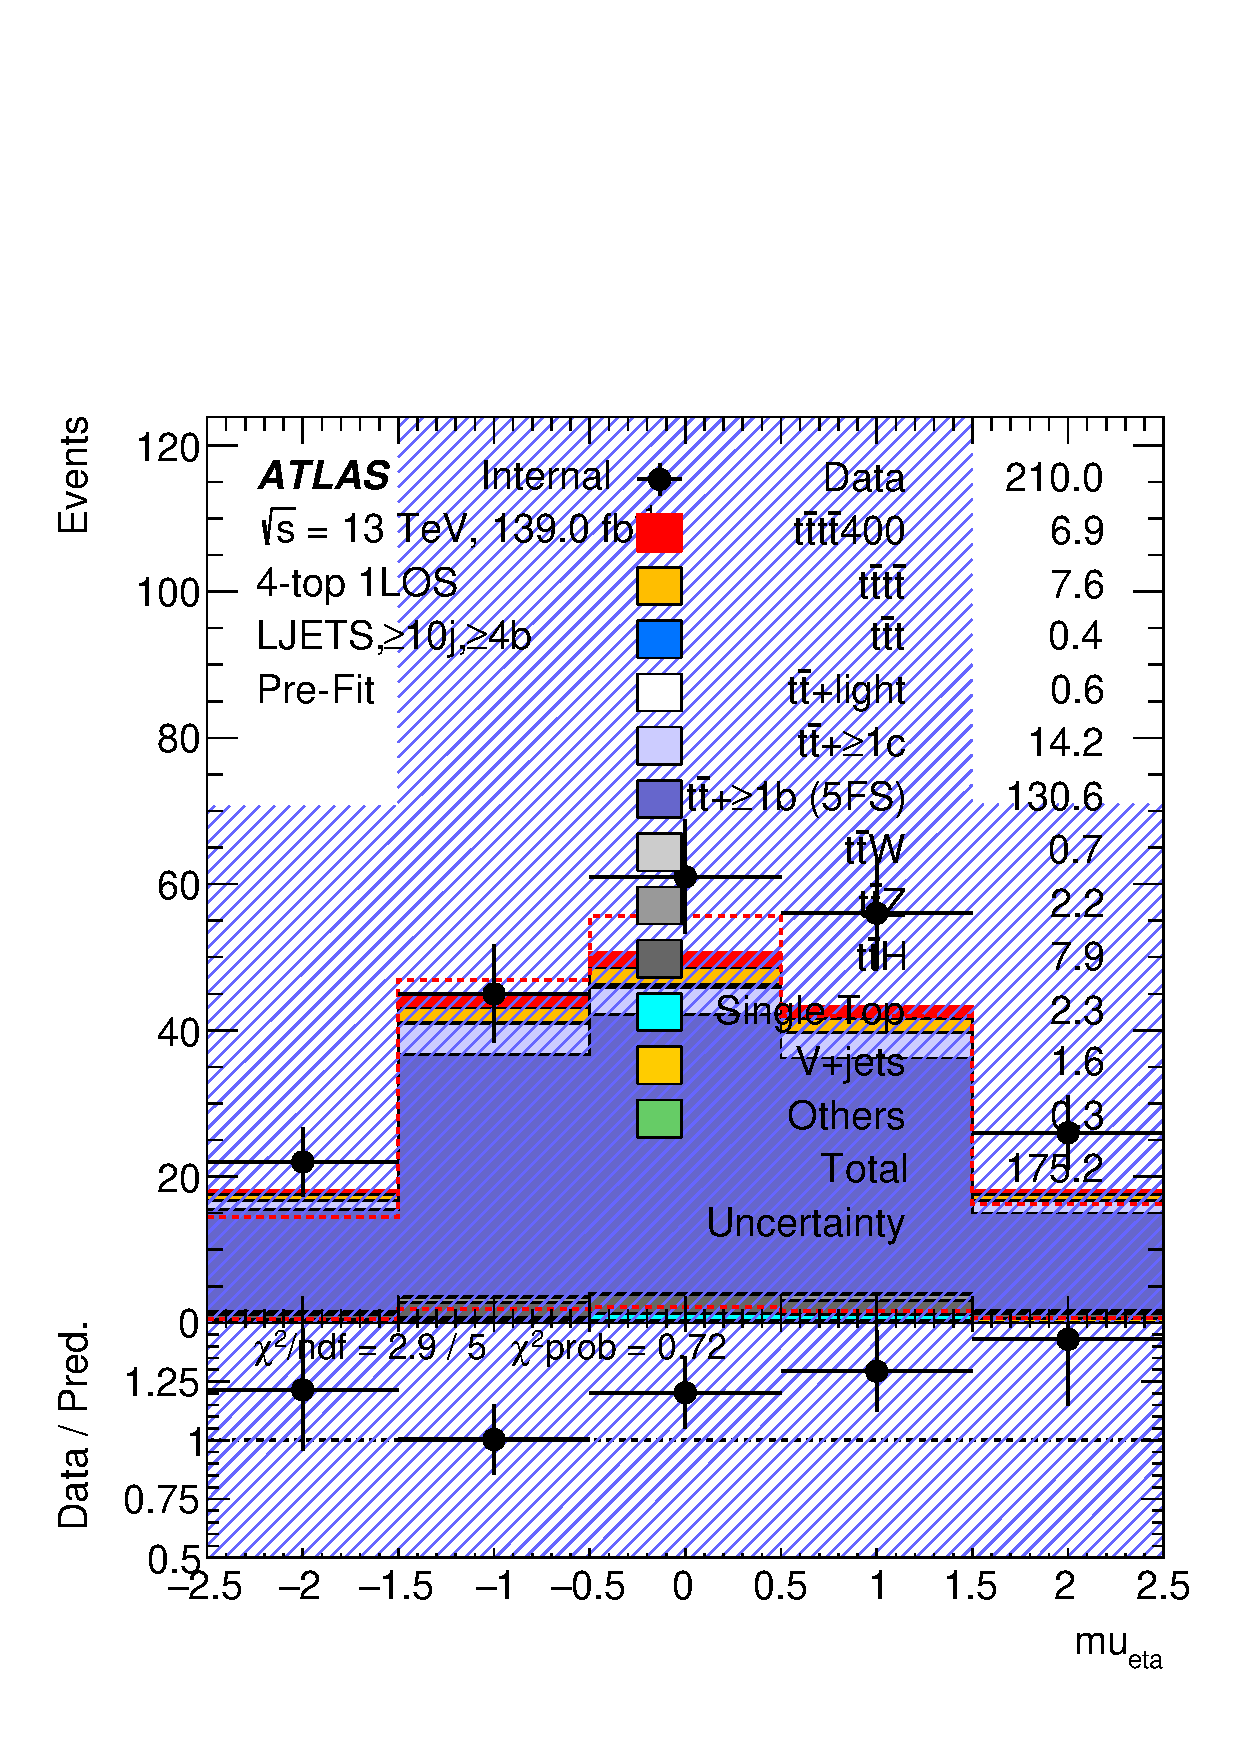
\includegraphics[width=0.23 \textwidth]{figures/fits/GNN/400/all/data_unblindedBonly/Plots/val_ljets_ge10j4b_mu_eta.pdf} &
        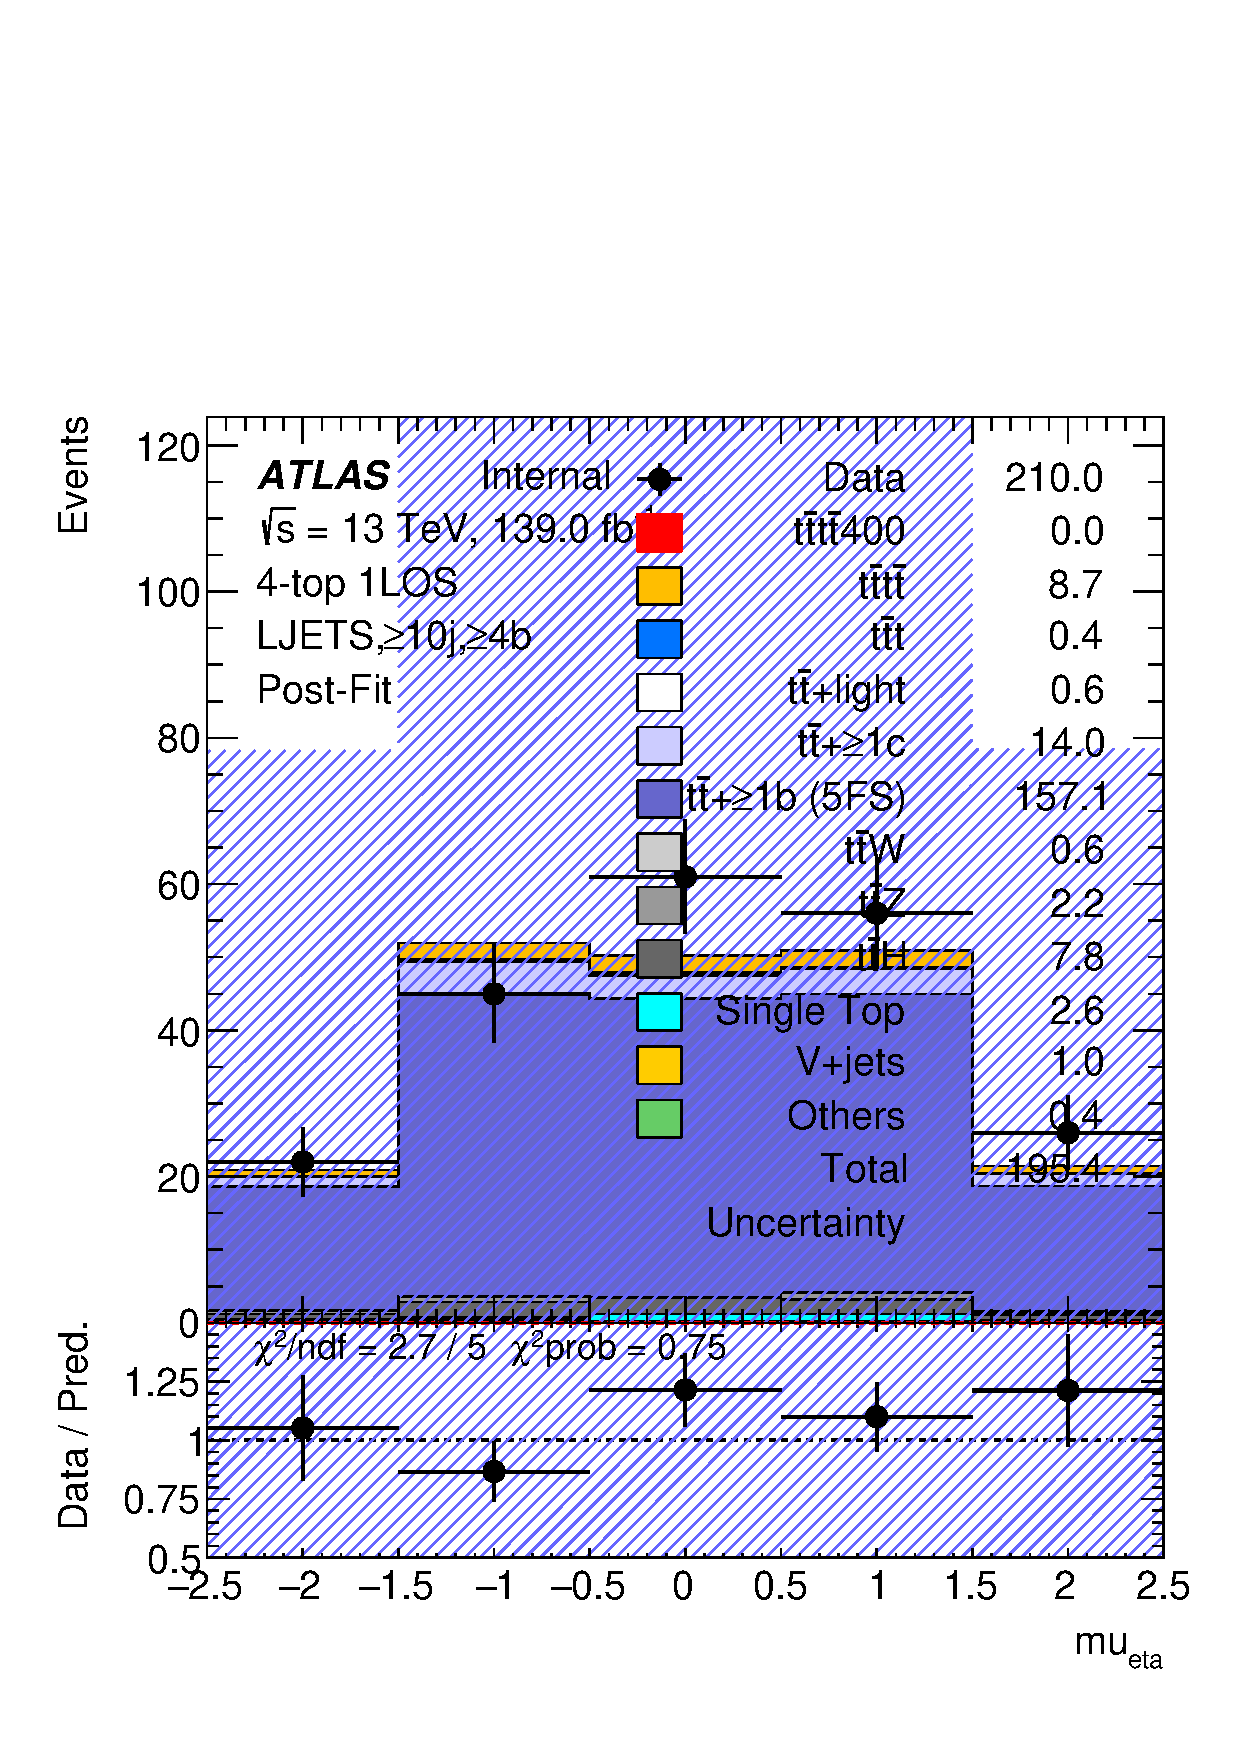
\includegraphics[width=0.23 \textwidth]{figures/fits/GNN/400/all/data_unblindedBonly/Plots/val_ljets_ge10j4b_mu_eta_postFit.pdf} &
        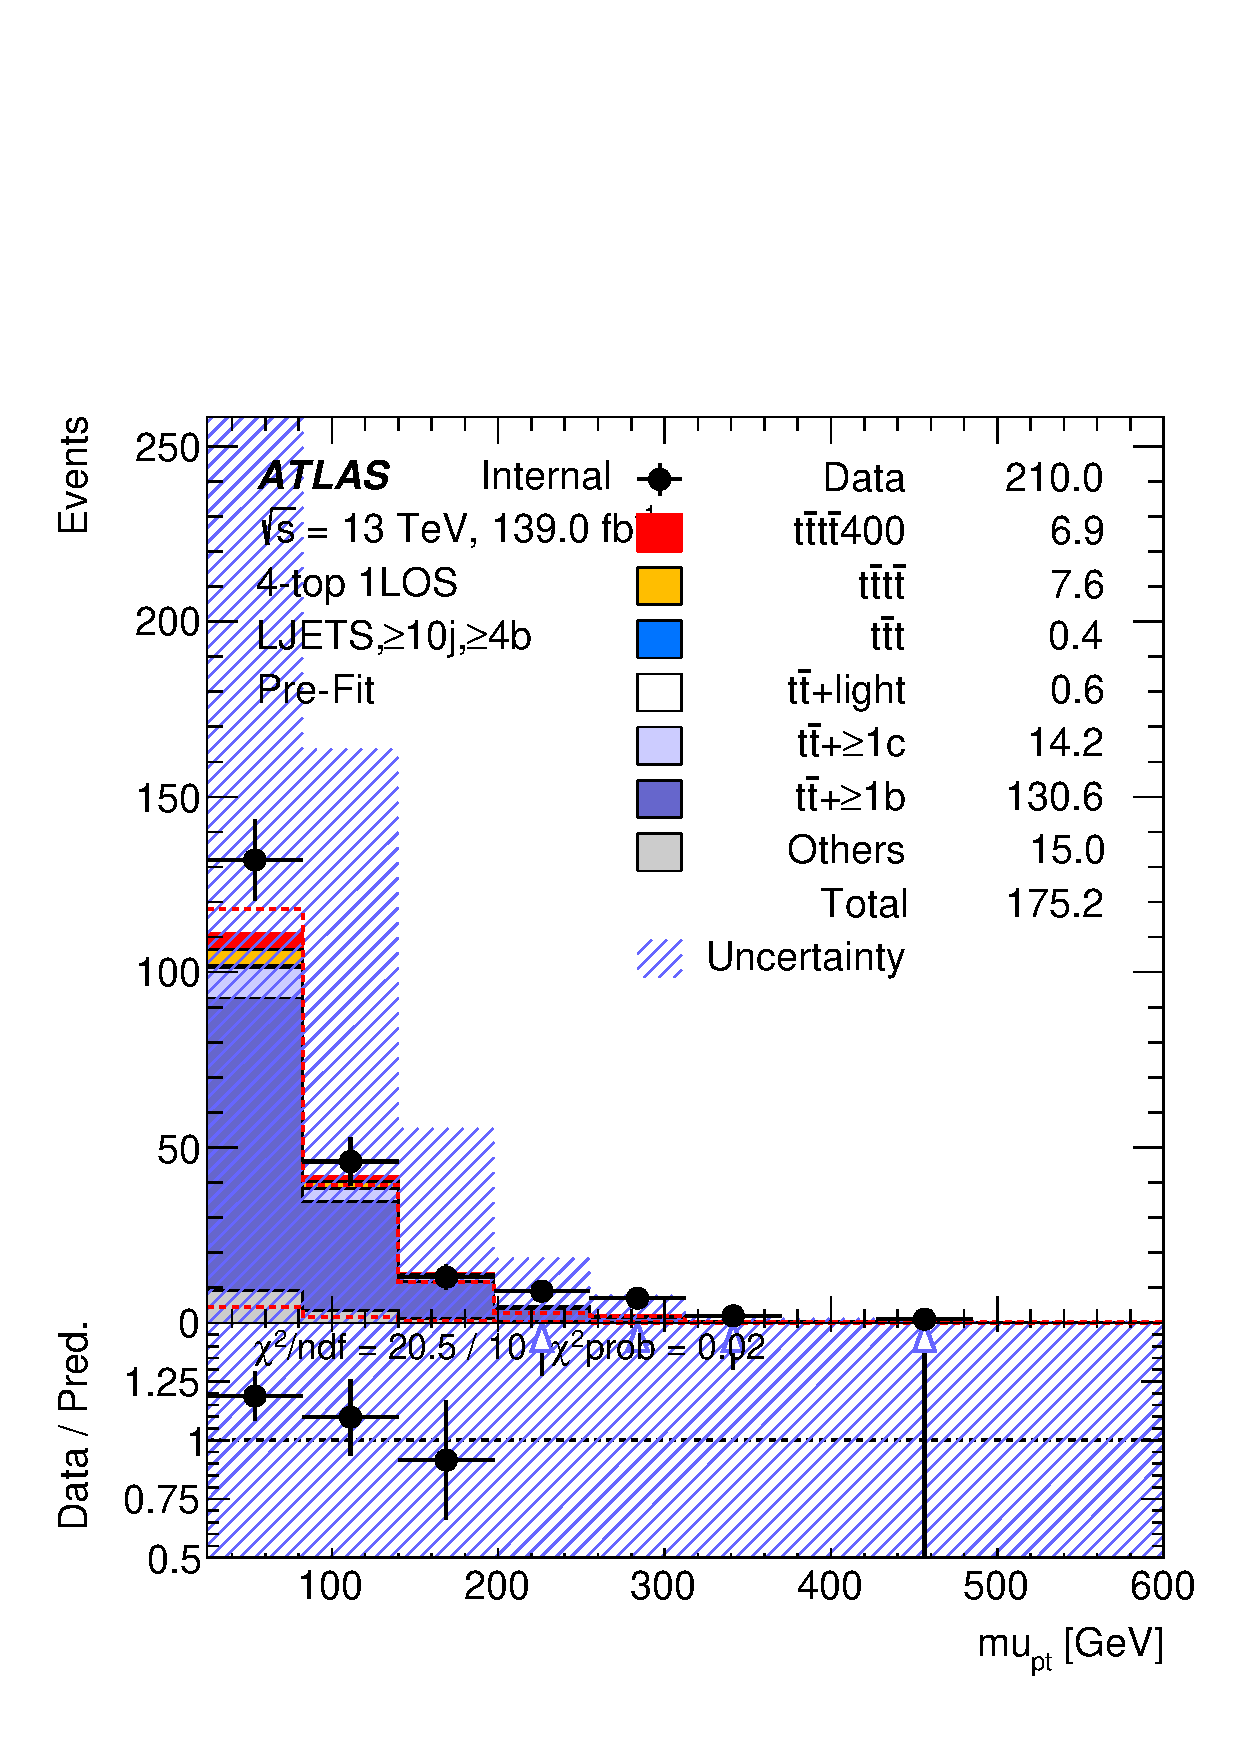
\includegraphics[width=0.23 \textwidth]{figures/fits/GNN/400/all/data_unblindedBonly/Plots/val_ljets_ge10j4b_mu_pt.pdf} &
        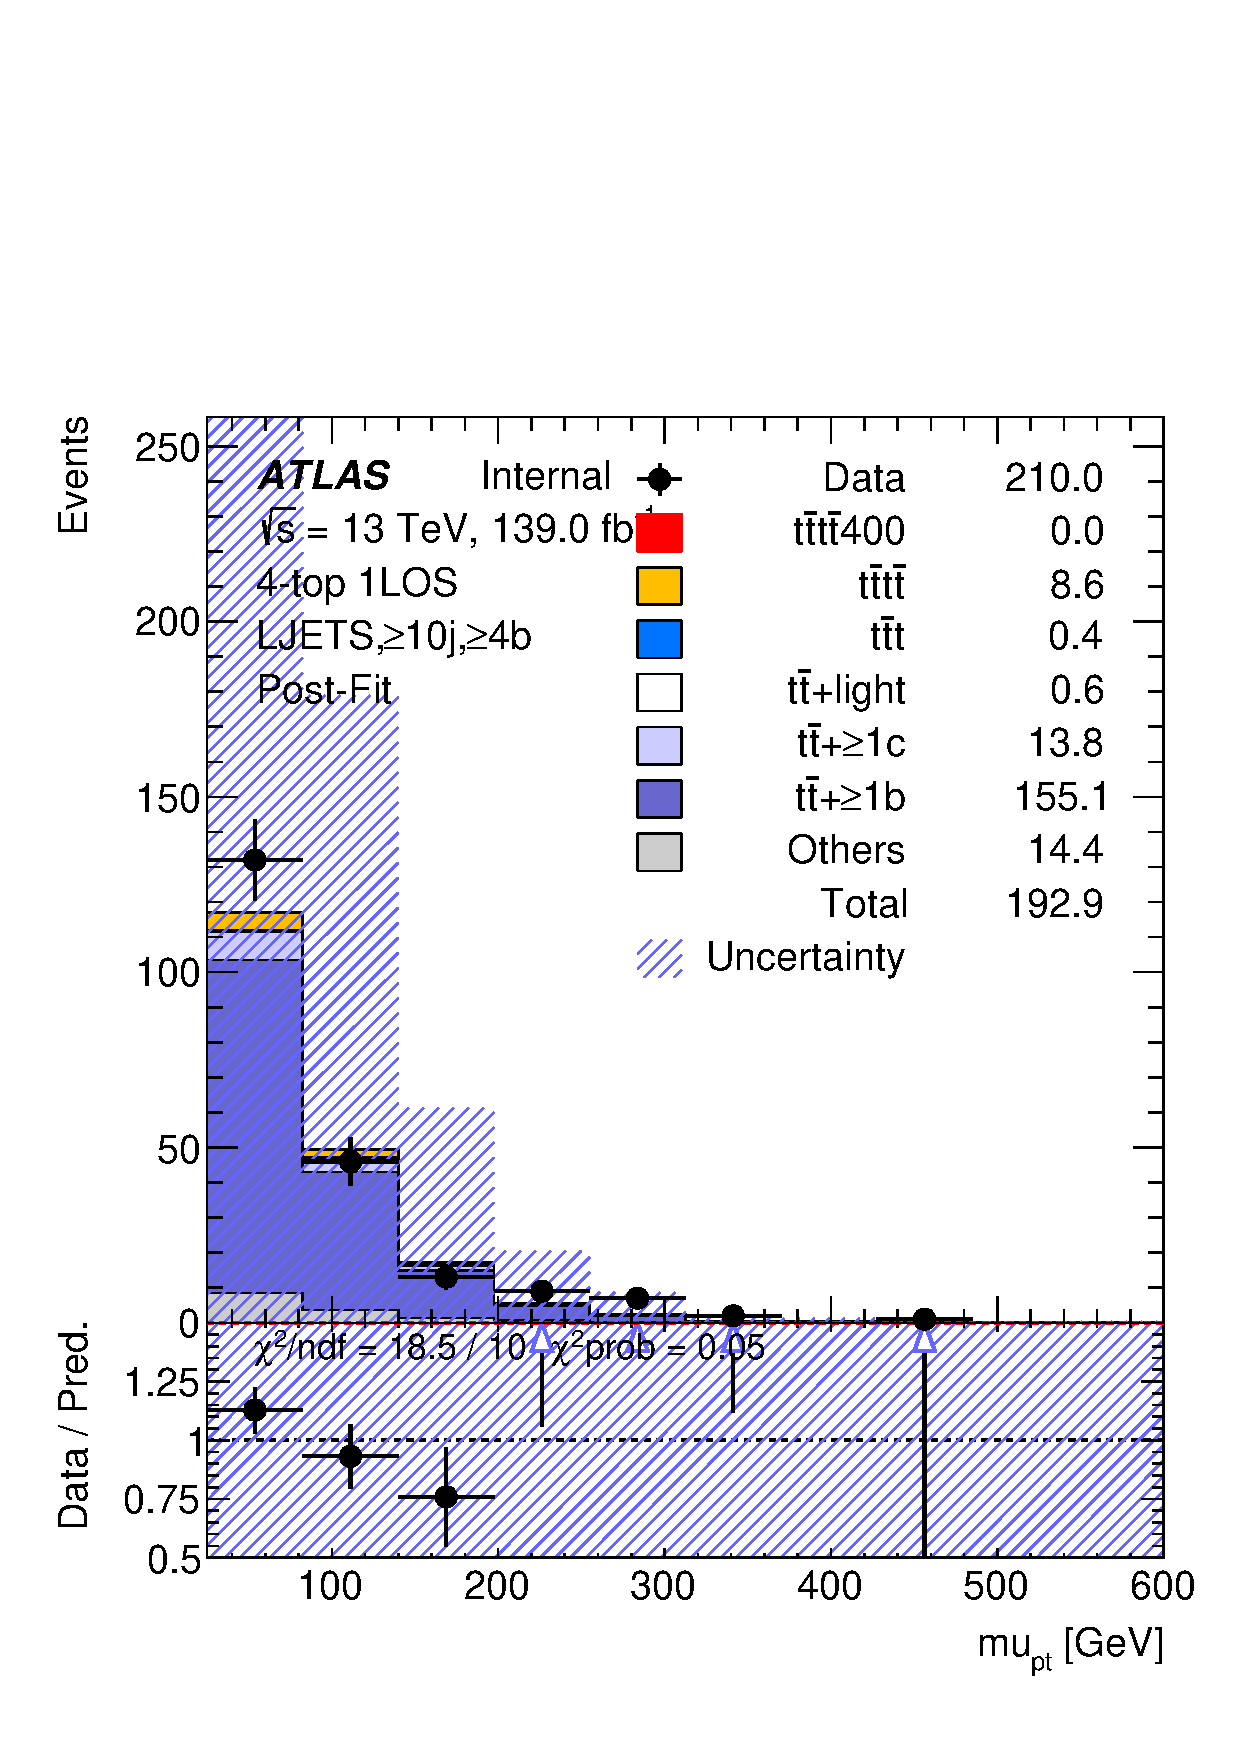
\includegraphics[width=0.23 \textwidth]{figures/fits/GNN/400/all/data_unblindedBonly/Plots/val_ljets_ge10j4b_mu_pt_postFit.pdf} \\

        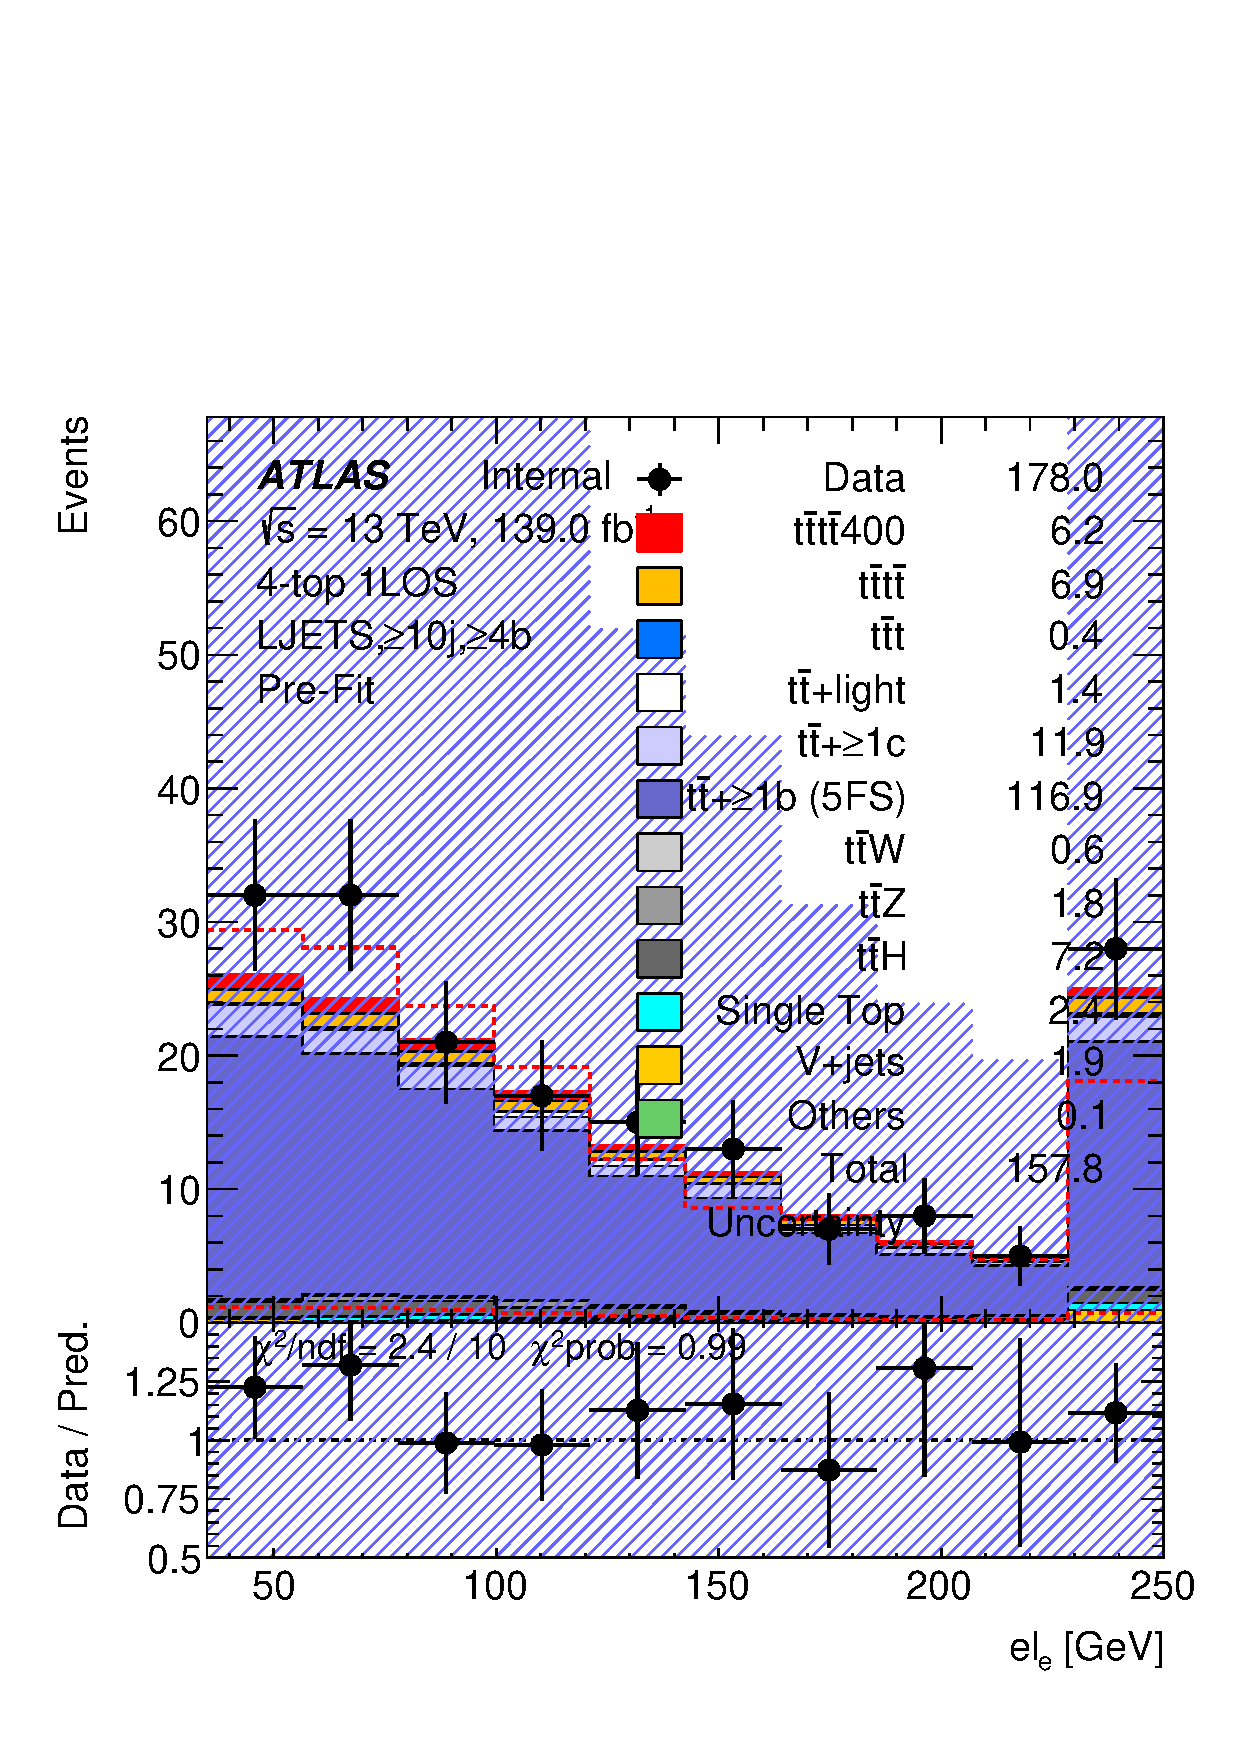
\includegraphics[width=0.23 \textwidth]{figures/fits/GNN/400/all/data_unblindedBonly/Plots/val_ljets_ge10j4b_el_e.pdf} &
        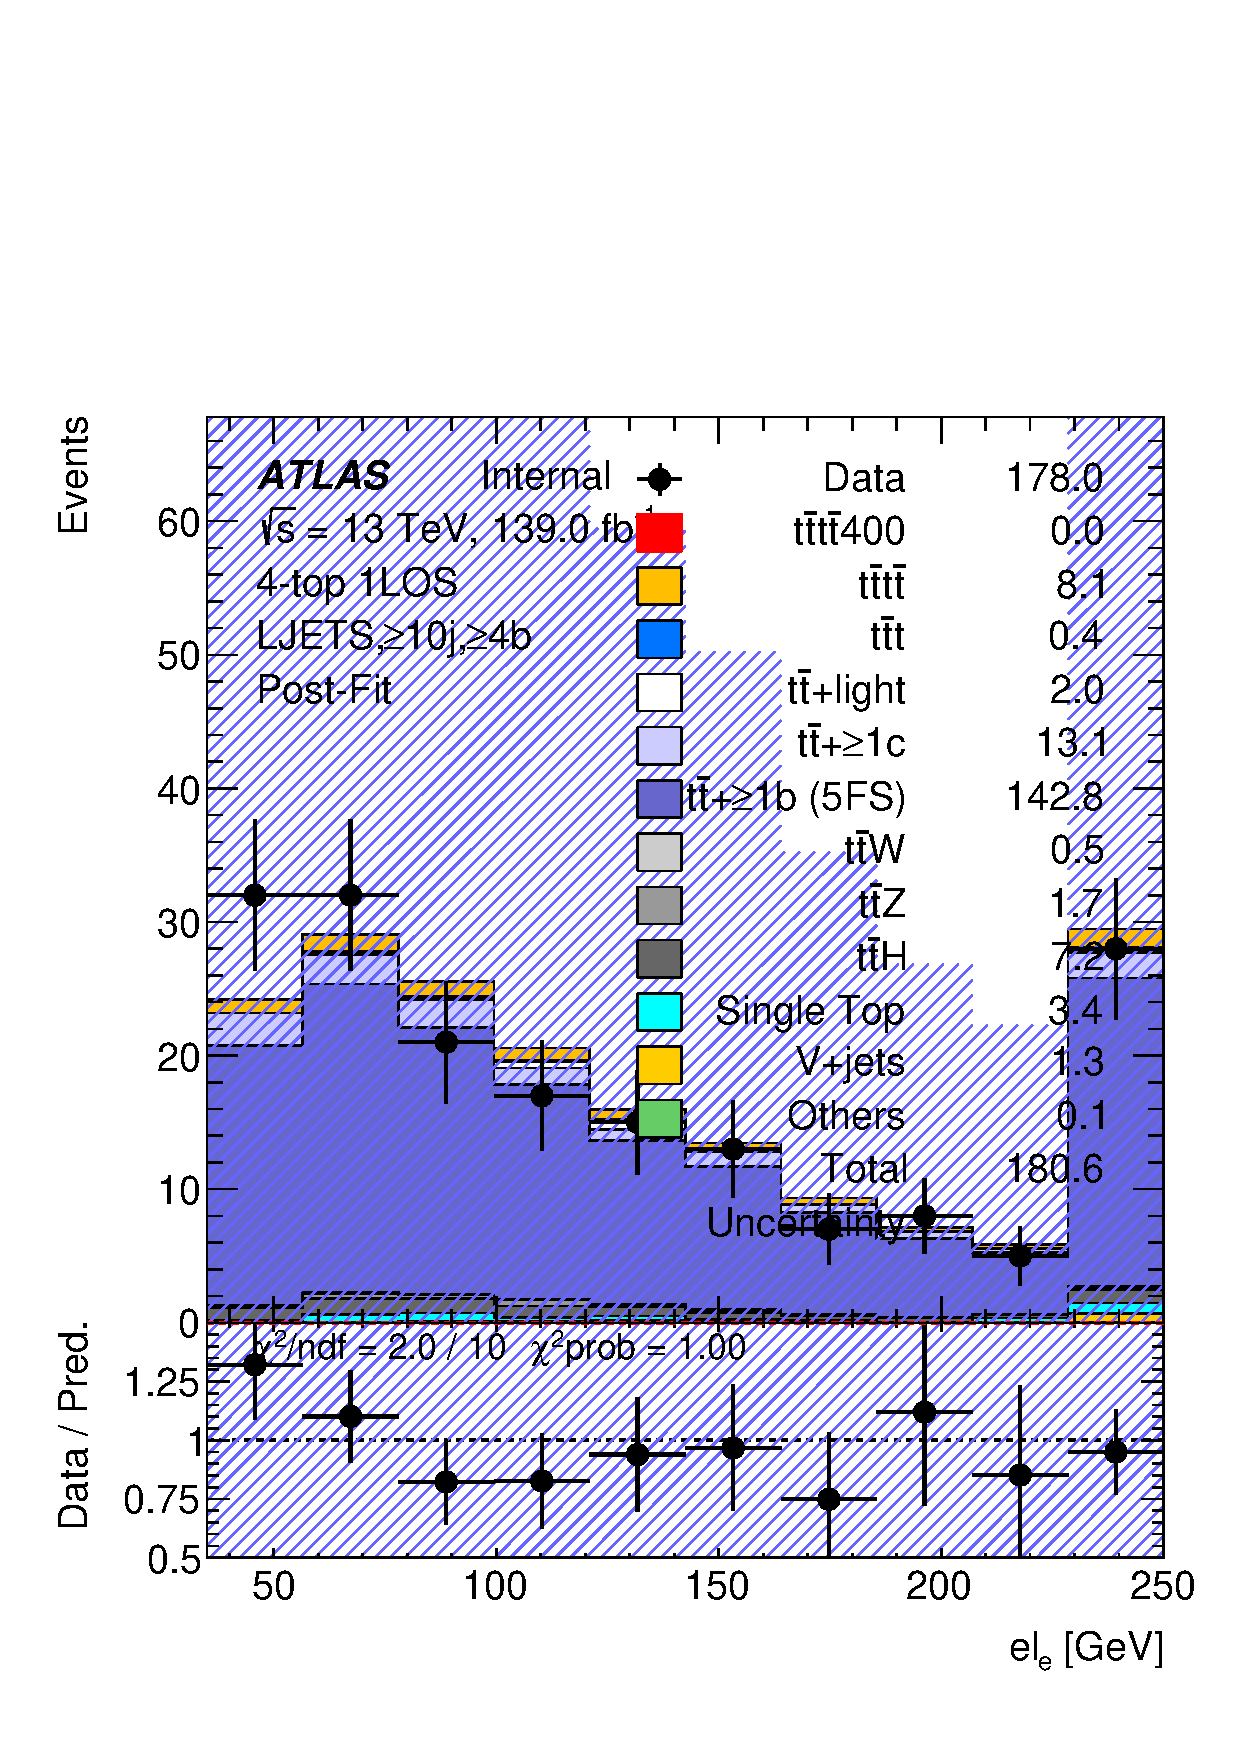
\includegraphics[width=0.23 \textwidth]{figures/fits/GNN/400/all/data_unblindedBonly/Plots/val_ljets_ge10j4b_el_e_postFit.pdf} &
        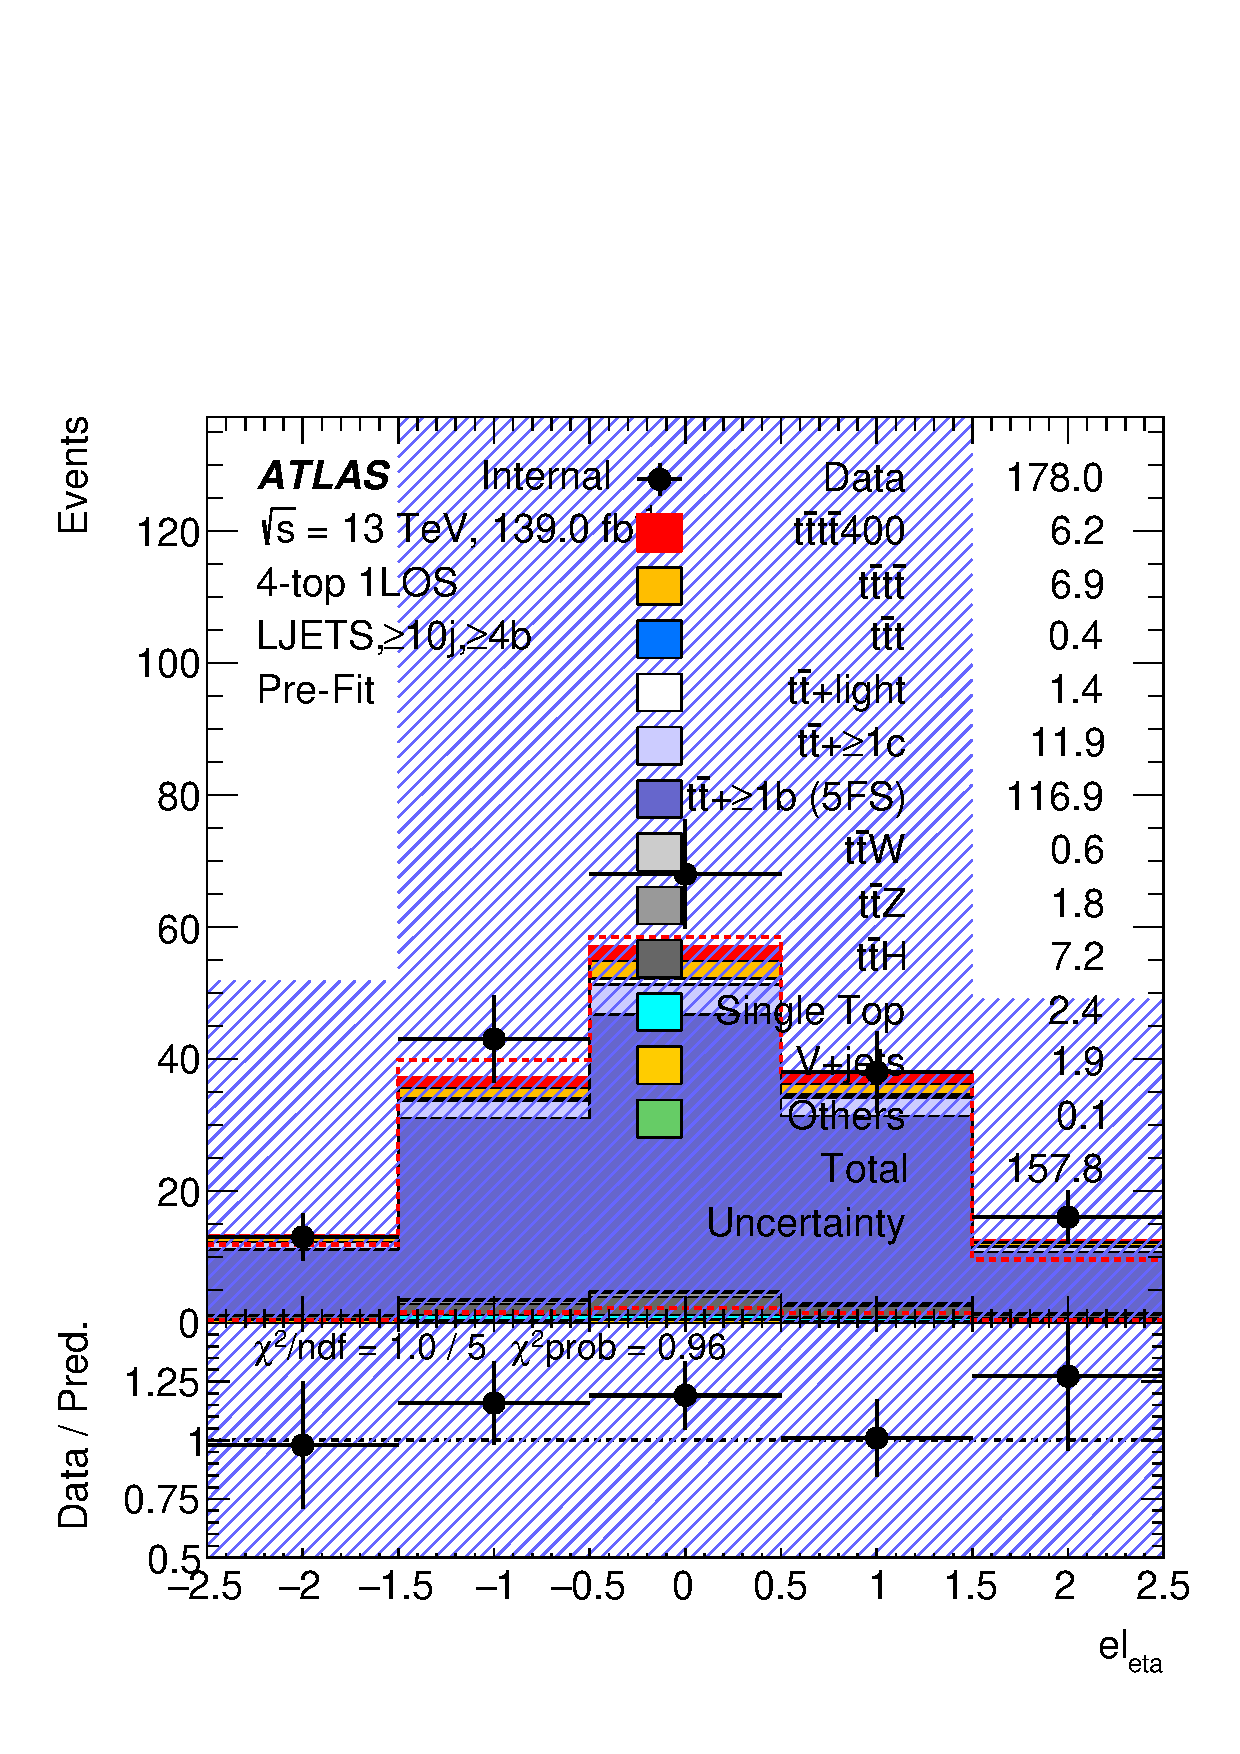
\includegraphics[width=0.23 \textwidth]{figures/fits/GNN/400/all/data_unblindedBonly/Plots/val_ljets_ge10j4b_el_eta.pdf} &
        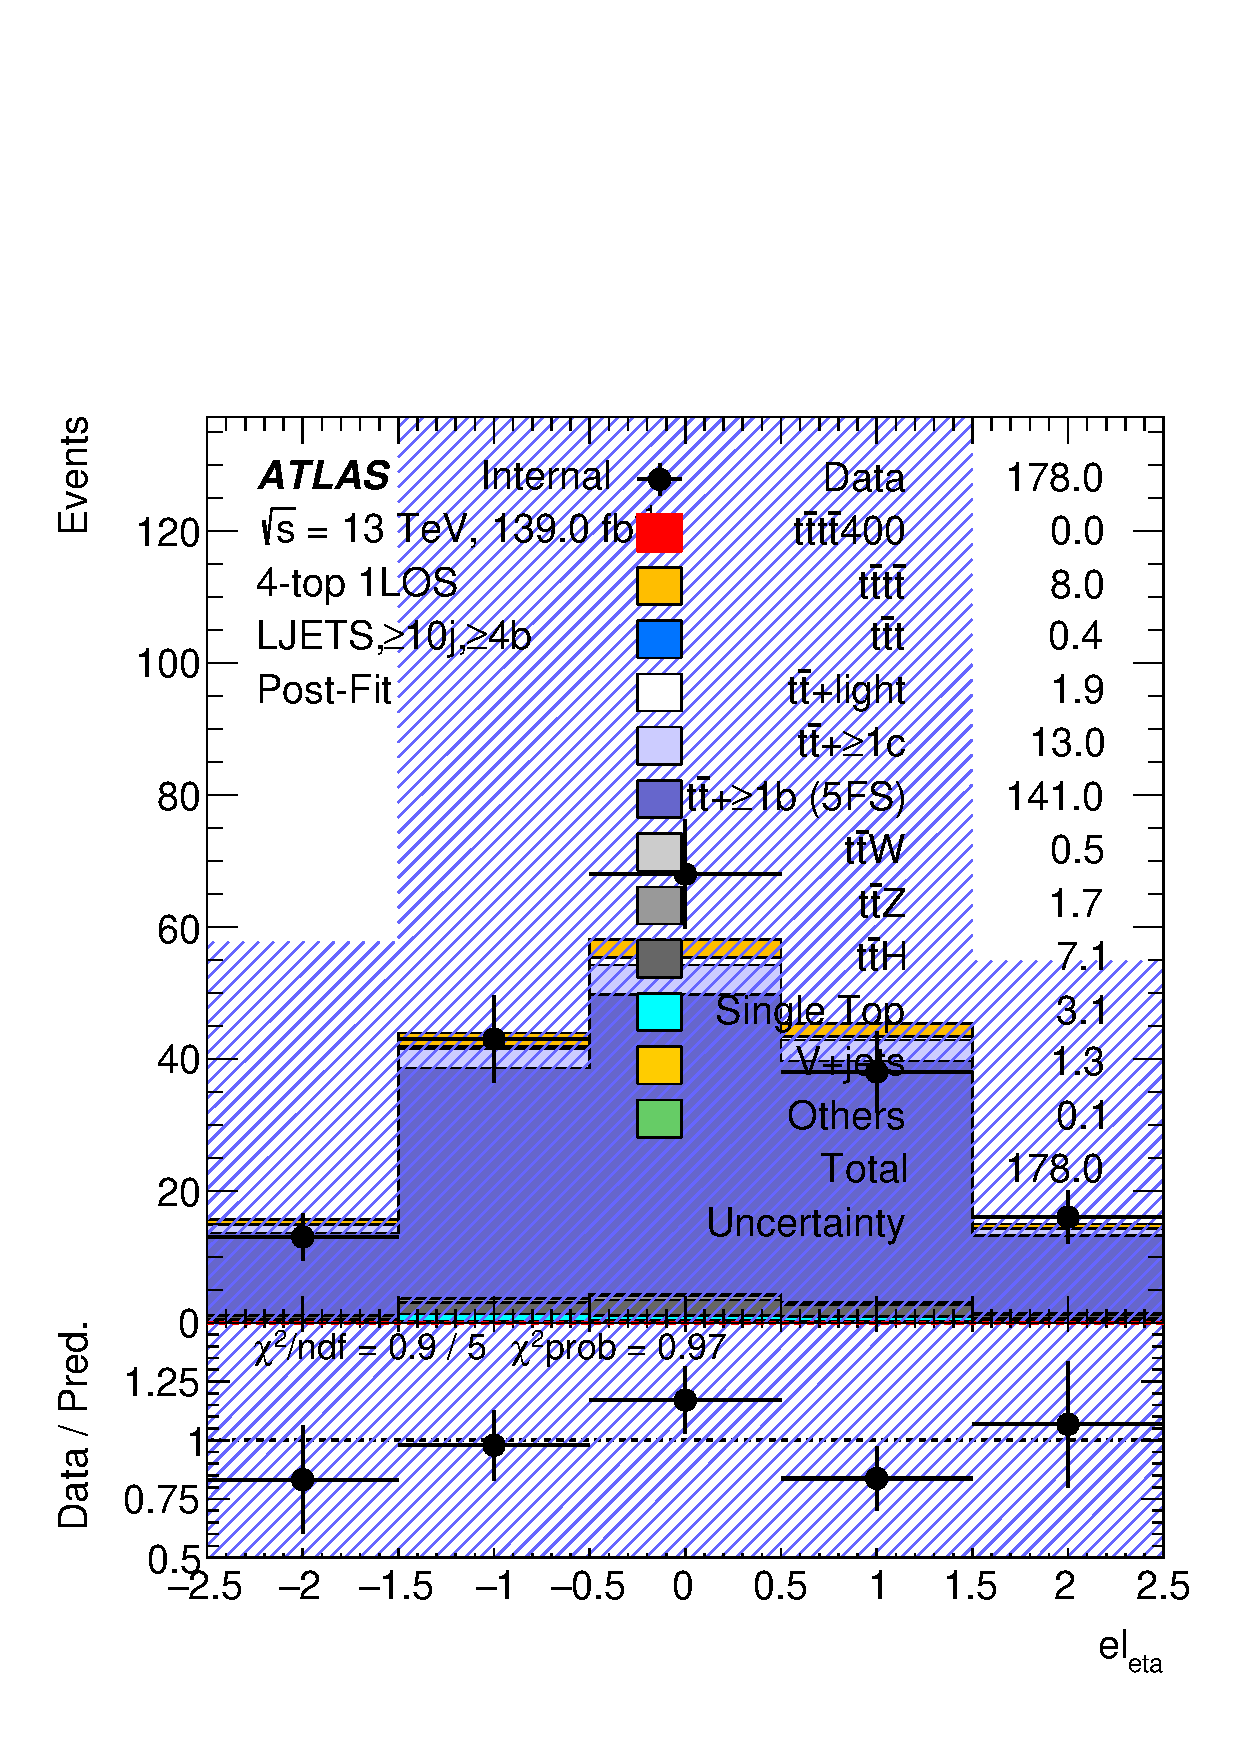
\includegraphics[width=0.23 \textwidth]{figures/fits/GNN/400/all/data_unblindedBonly/Plots/val_ljets_ge10j4b_el_eta_postFit.pdf} \\

        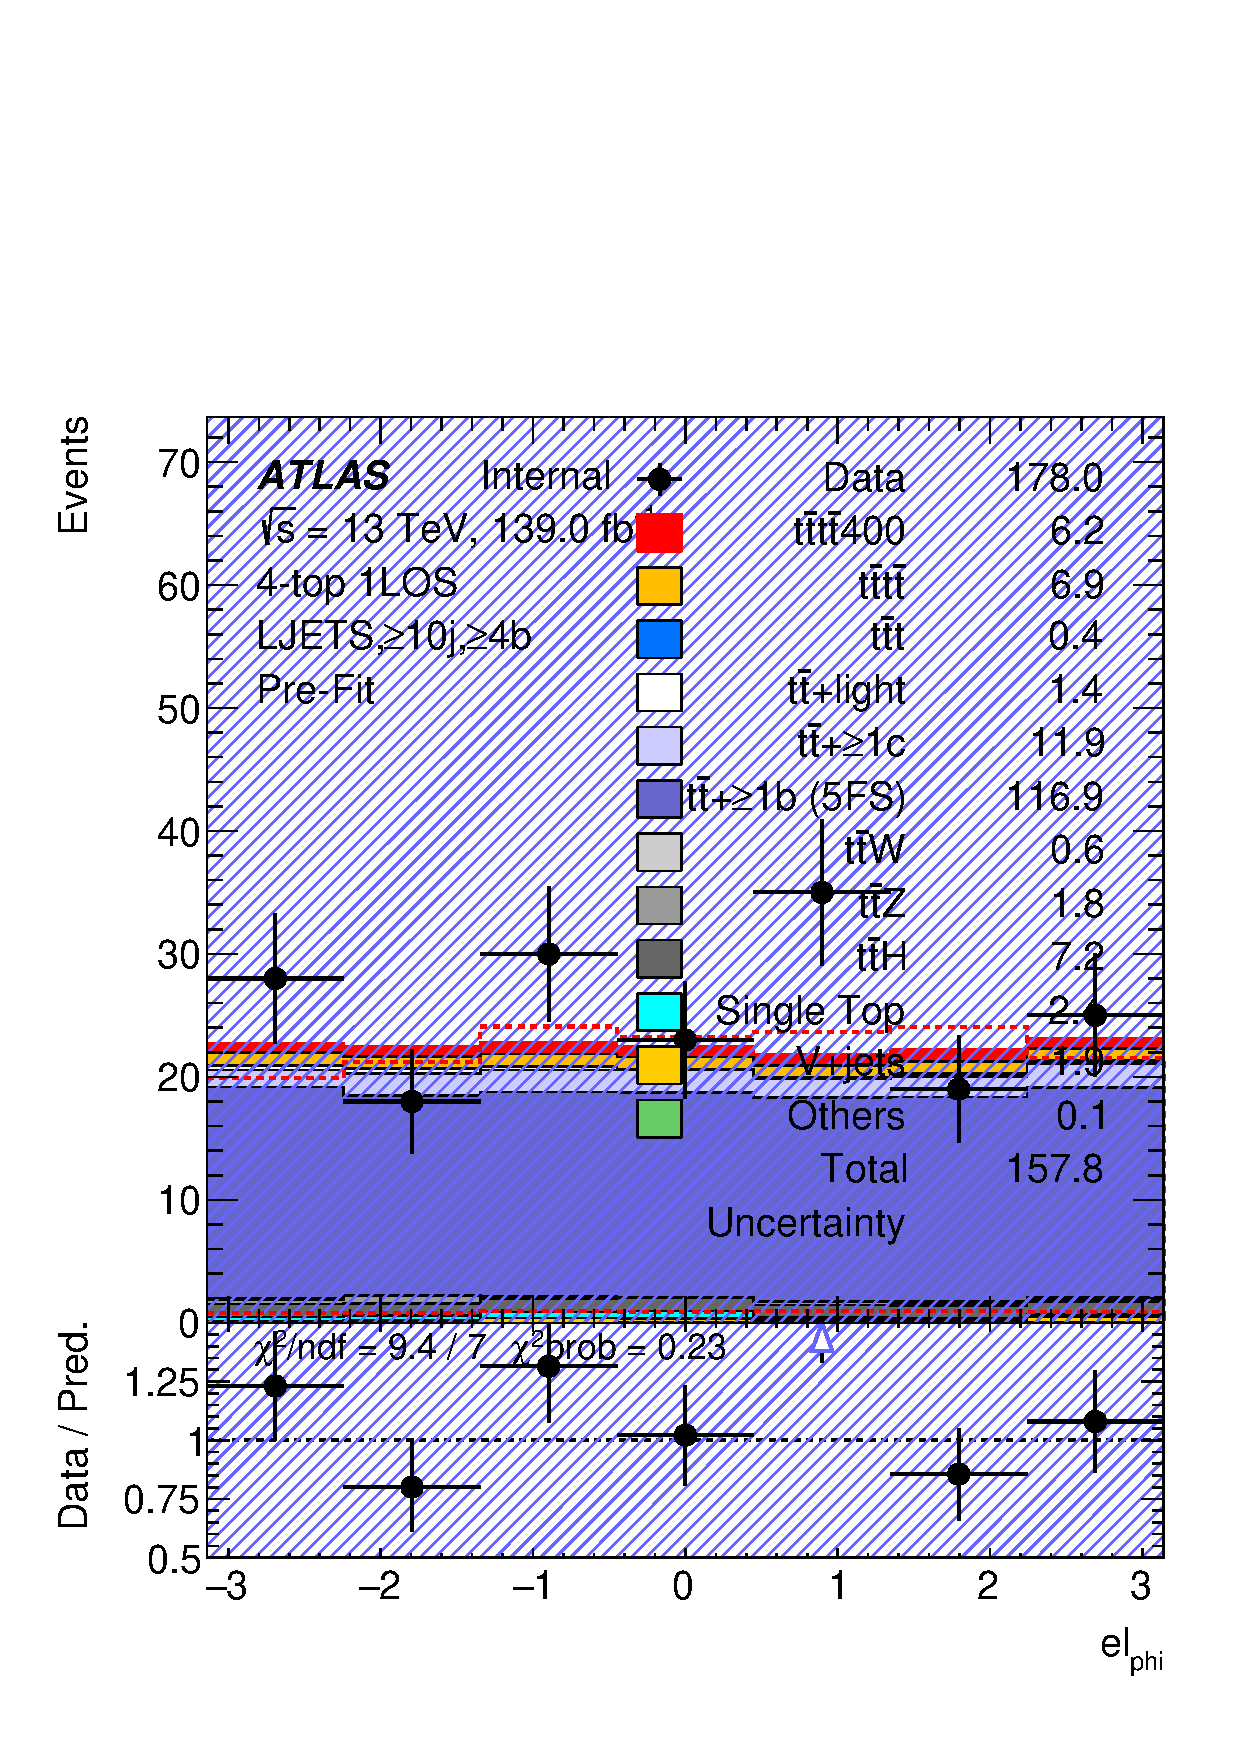
\includegraphics[width=0.23 \textwidth]{figures/fits/GNN/400/all/data_unblindedBonly/Plots/val_ljets_ge10j4b_el_phi.pdf} &
        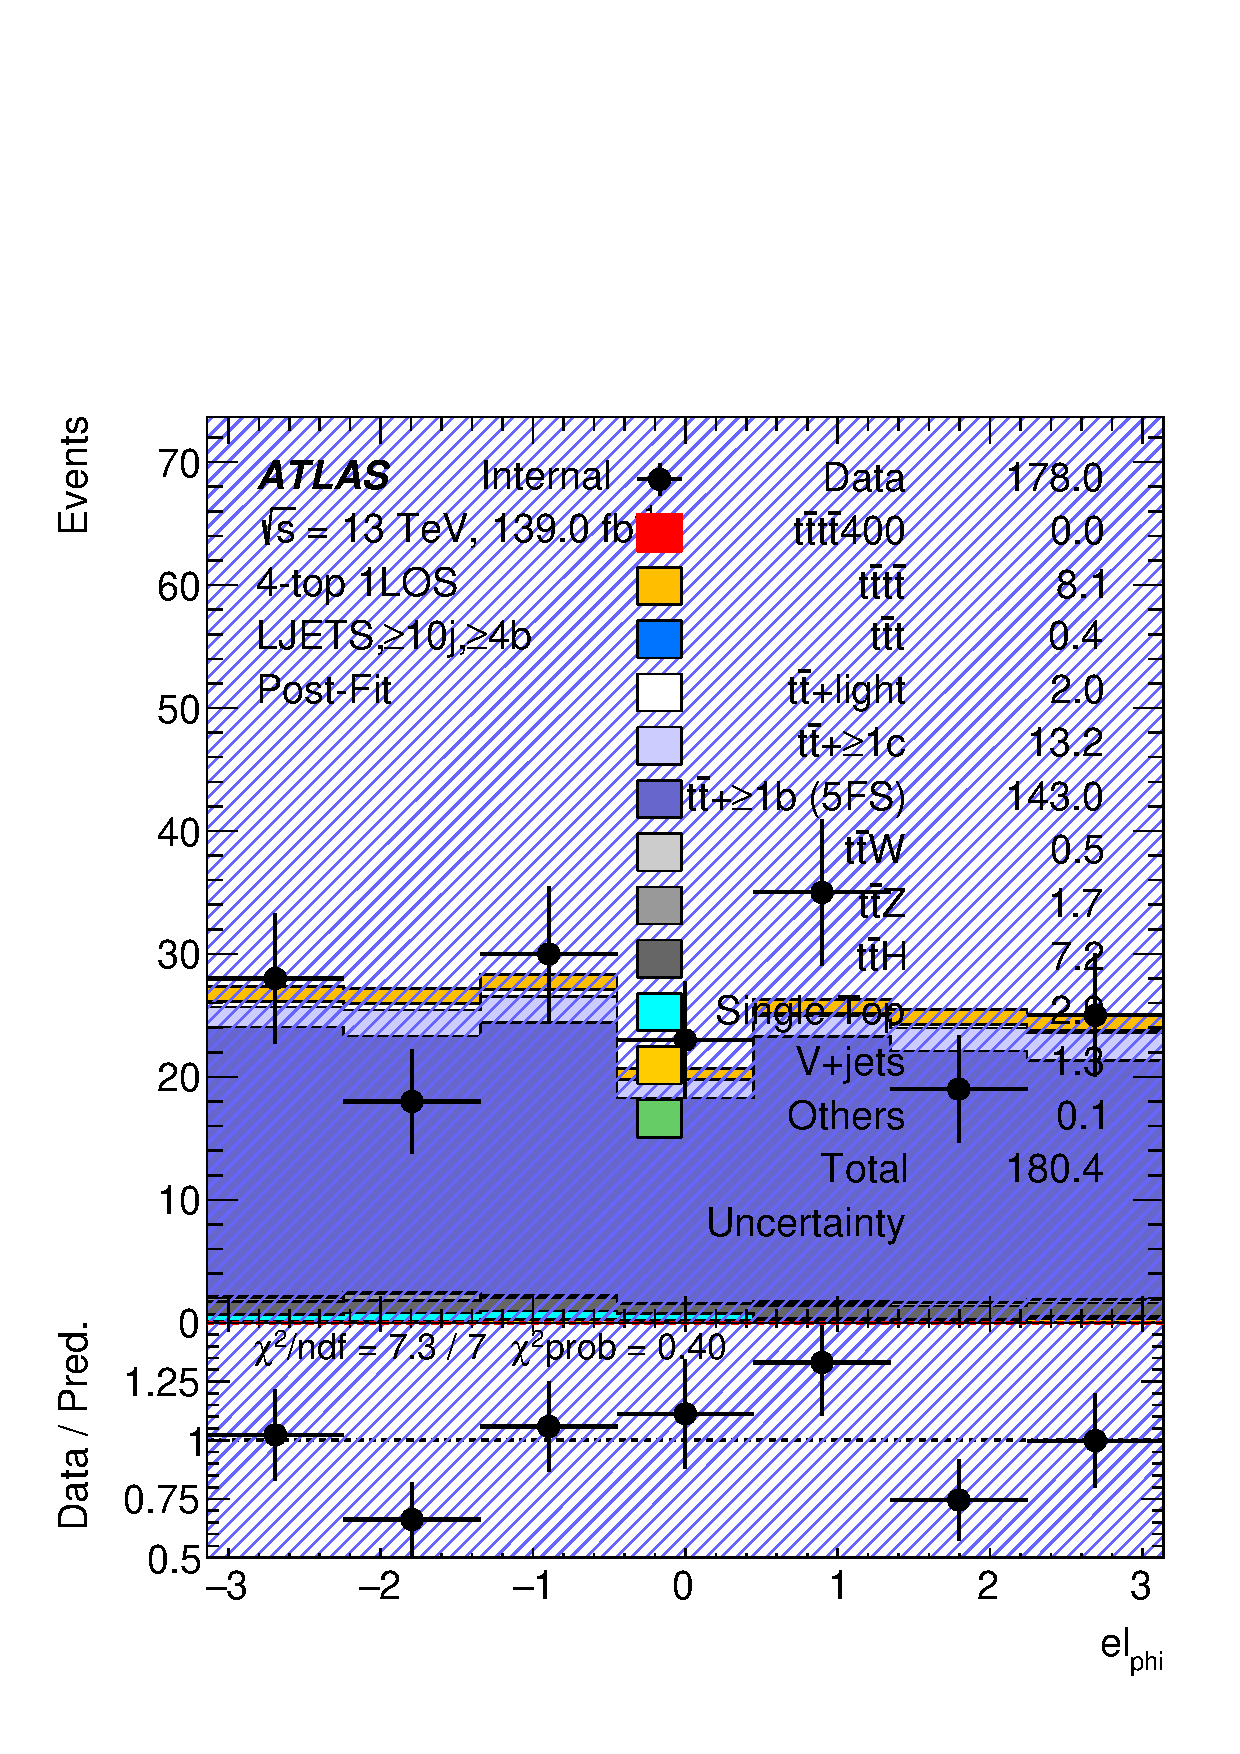
\includegraphics[width=0.23 \textwidth]{figures/fits/GNN/400/all/data_unblindedBonly/Plots/val_ljets_ge10j4b_el_phi_postFit.pdf} &
        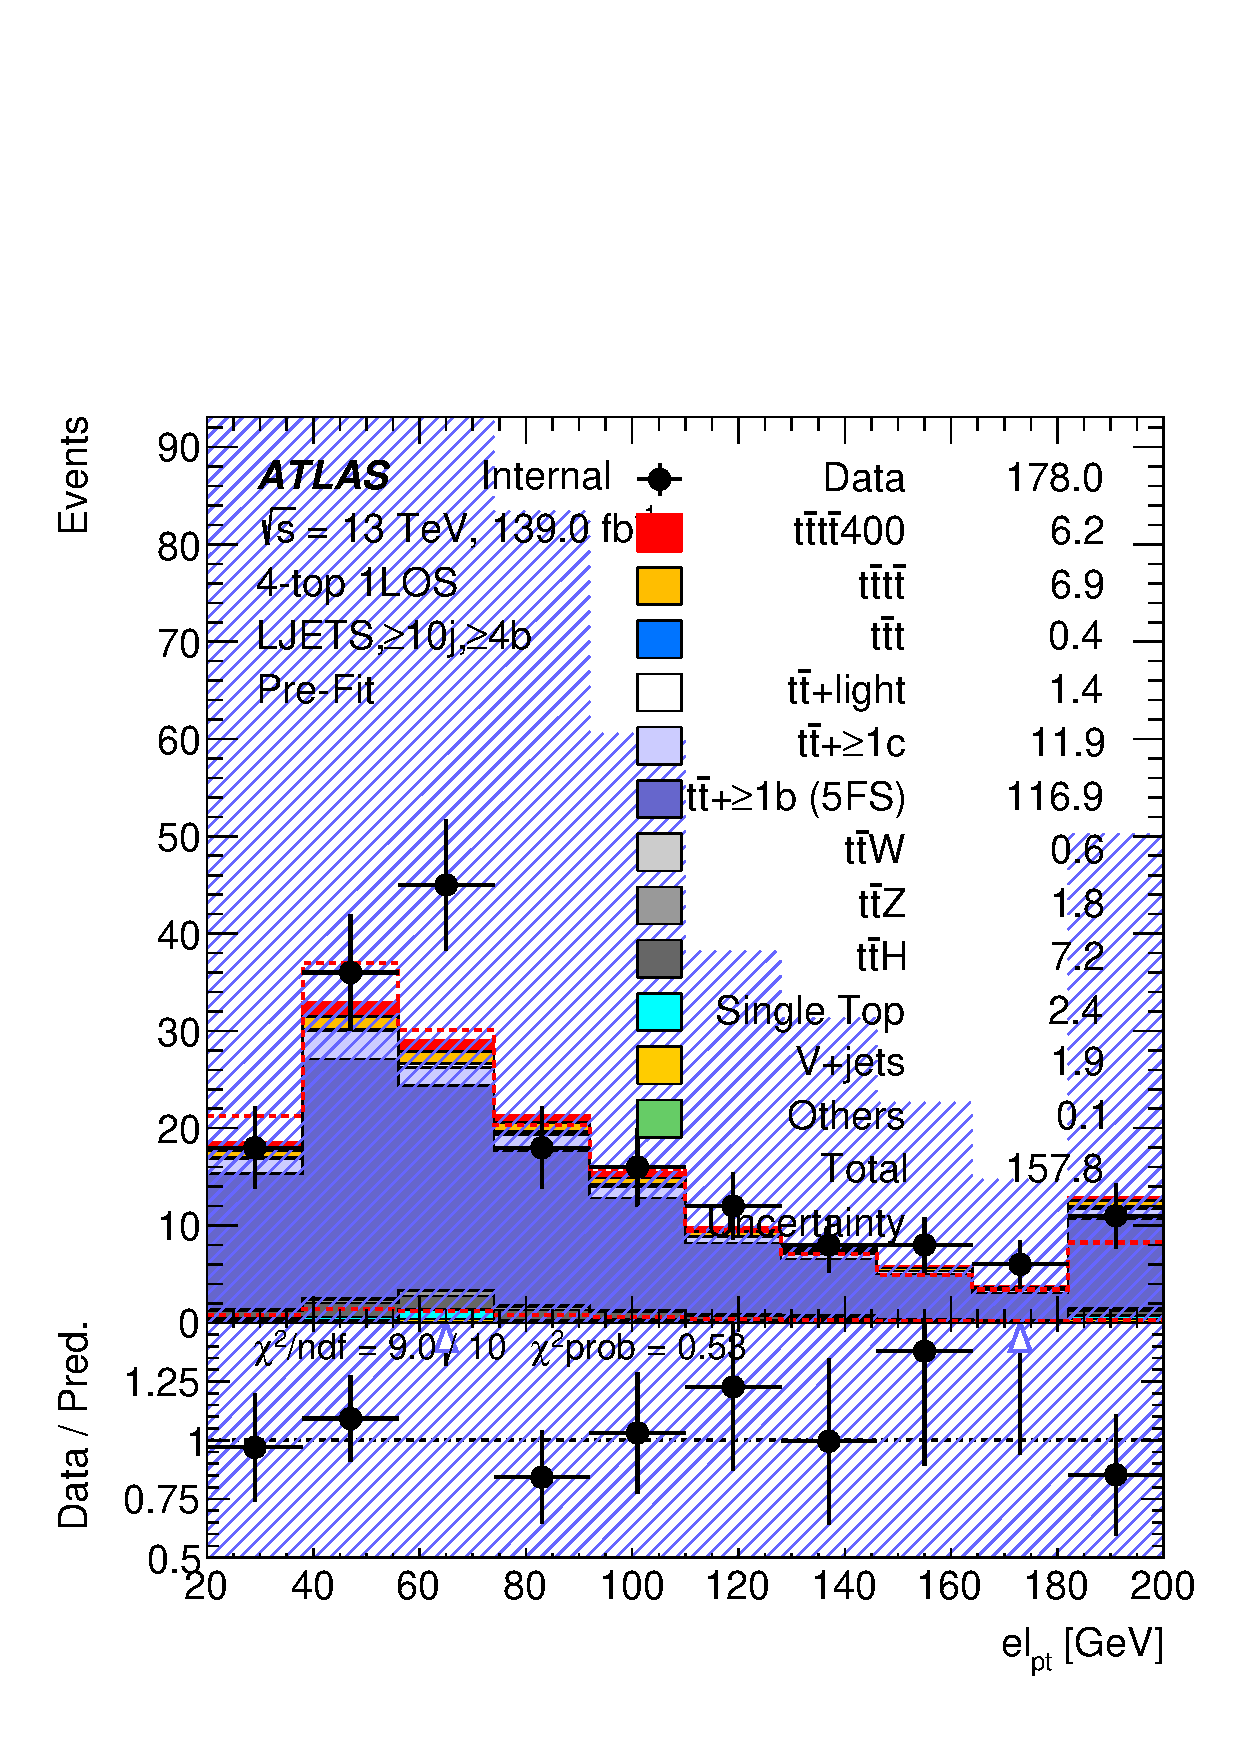
\includegraphics[width=0.23 \textwidth]{figures/fits/GNN/400/all/data_unblindedBonly/Plots/val_ljets_ge10j4b_el_pt.pdf} &
        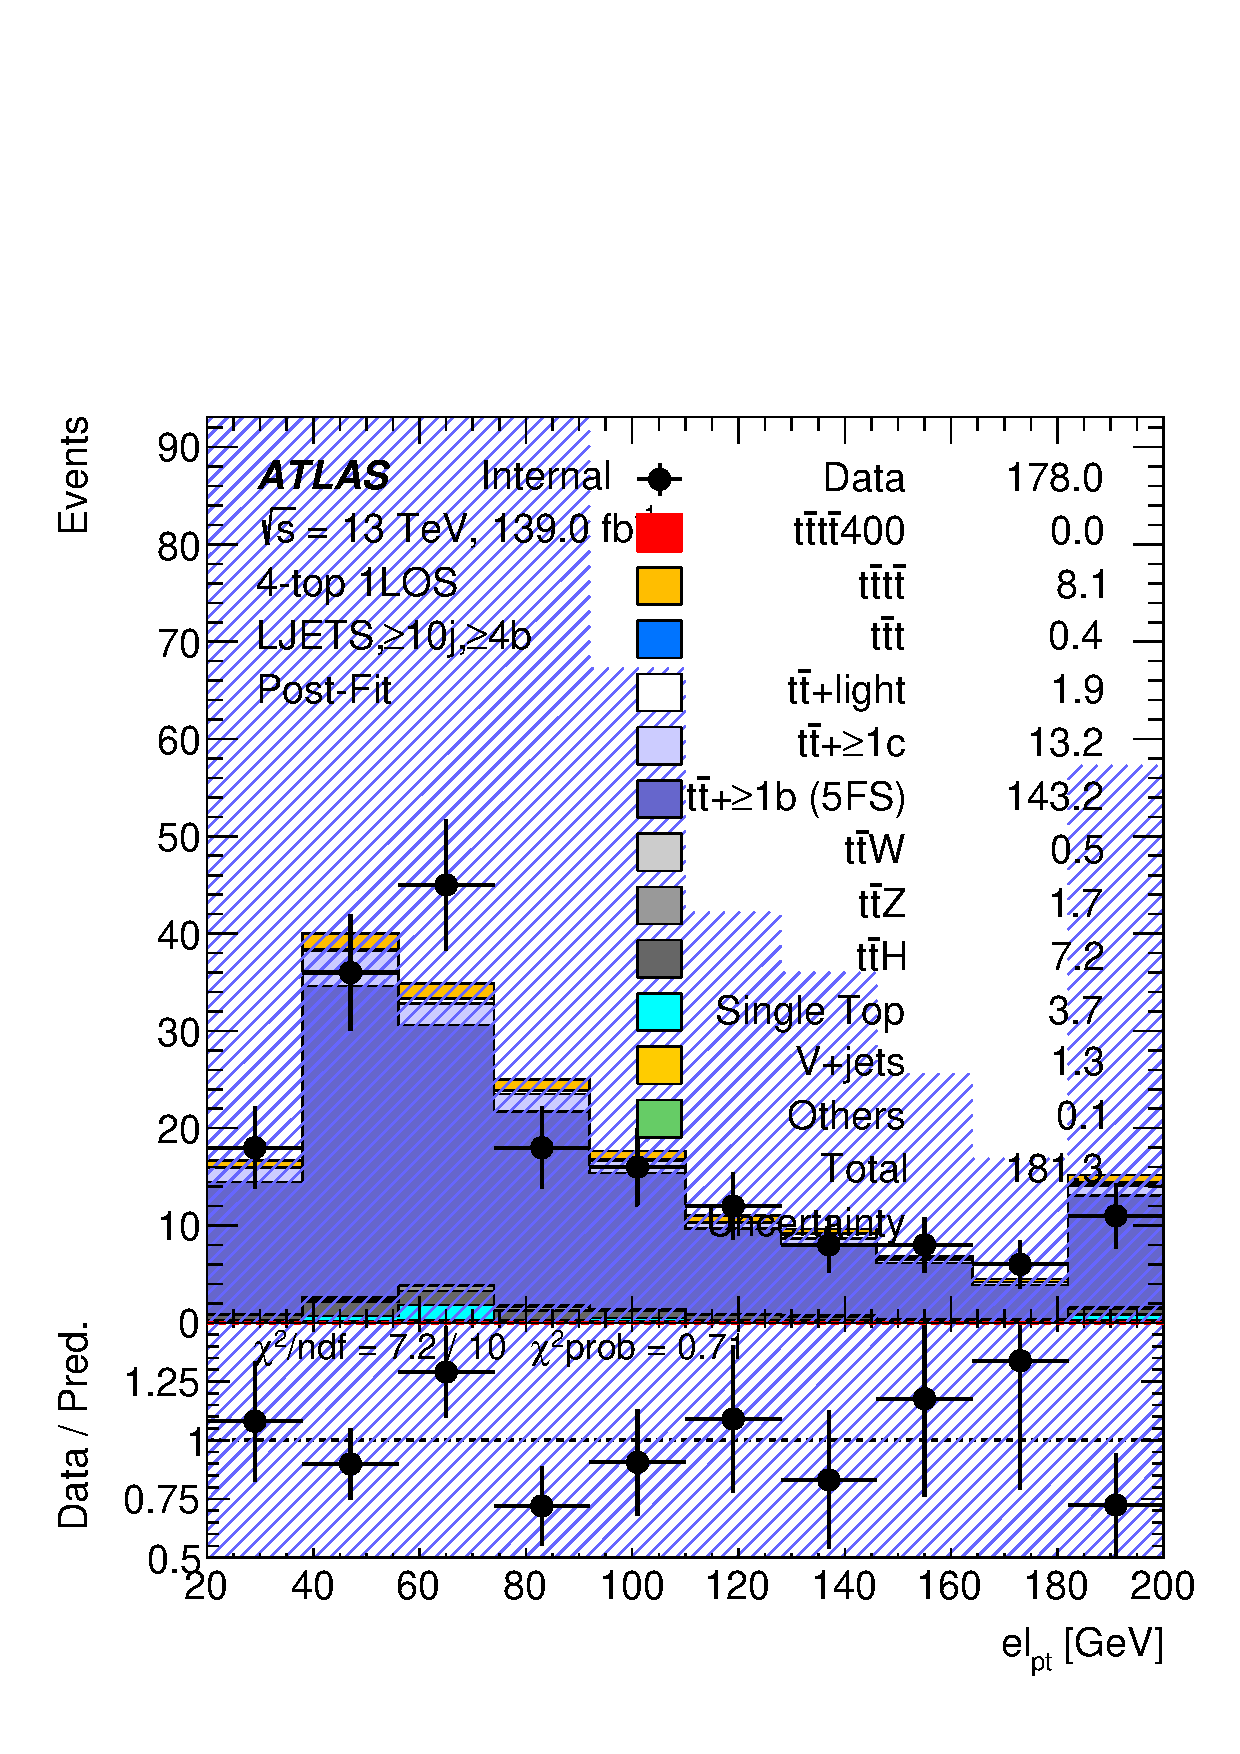
\includegraphics[width=0.23 \textwidth]{figures/fits/GNN/400/all/data_unblindedBonly/Plots/val_ljets_ge10j4b_el_pt_postFit.pdf} \\

        \end{tabular}
        \end{center}

\caption{\label{GNN_input_val_3}Pre-fit(left) and Post-fit(right) distributions for GNN input variables in the ge10j4b region.}
\end{figure}



\clearpage

\subsection{GNN Input Variable Distributions for region 2L, $\geq8$ jets, 3bL}
\label{app:validation_GNN_input_2L_ge8j3bL}

The pre-fit and post-fit plots for the GNN input variables are shown in Figures \ref{GNN_input_val_1}, \ref{GNN_input_val_2}, and \ref{GNN_input_val_3} from the background-only unblinded-data fits. The distributions are shown for the 2L ge8j3bL region, which is one of the regions most sensitive to signal. Good MC/data agreement can be seen.

\begin{figure}
        \begin{center} \setlength{\tabcolsep}{2.5pt}\footnotesize
        \begin{tabular}{cccc}
        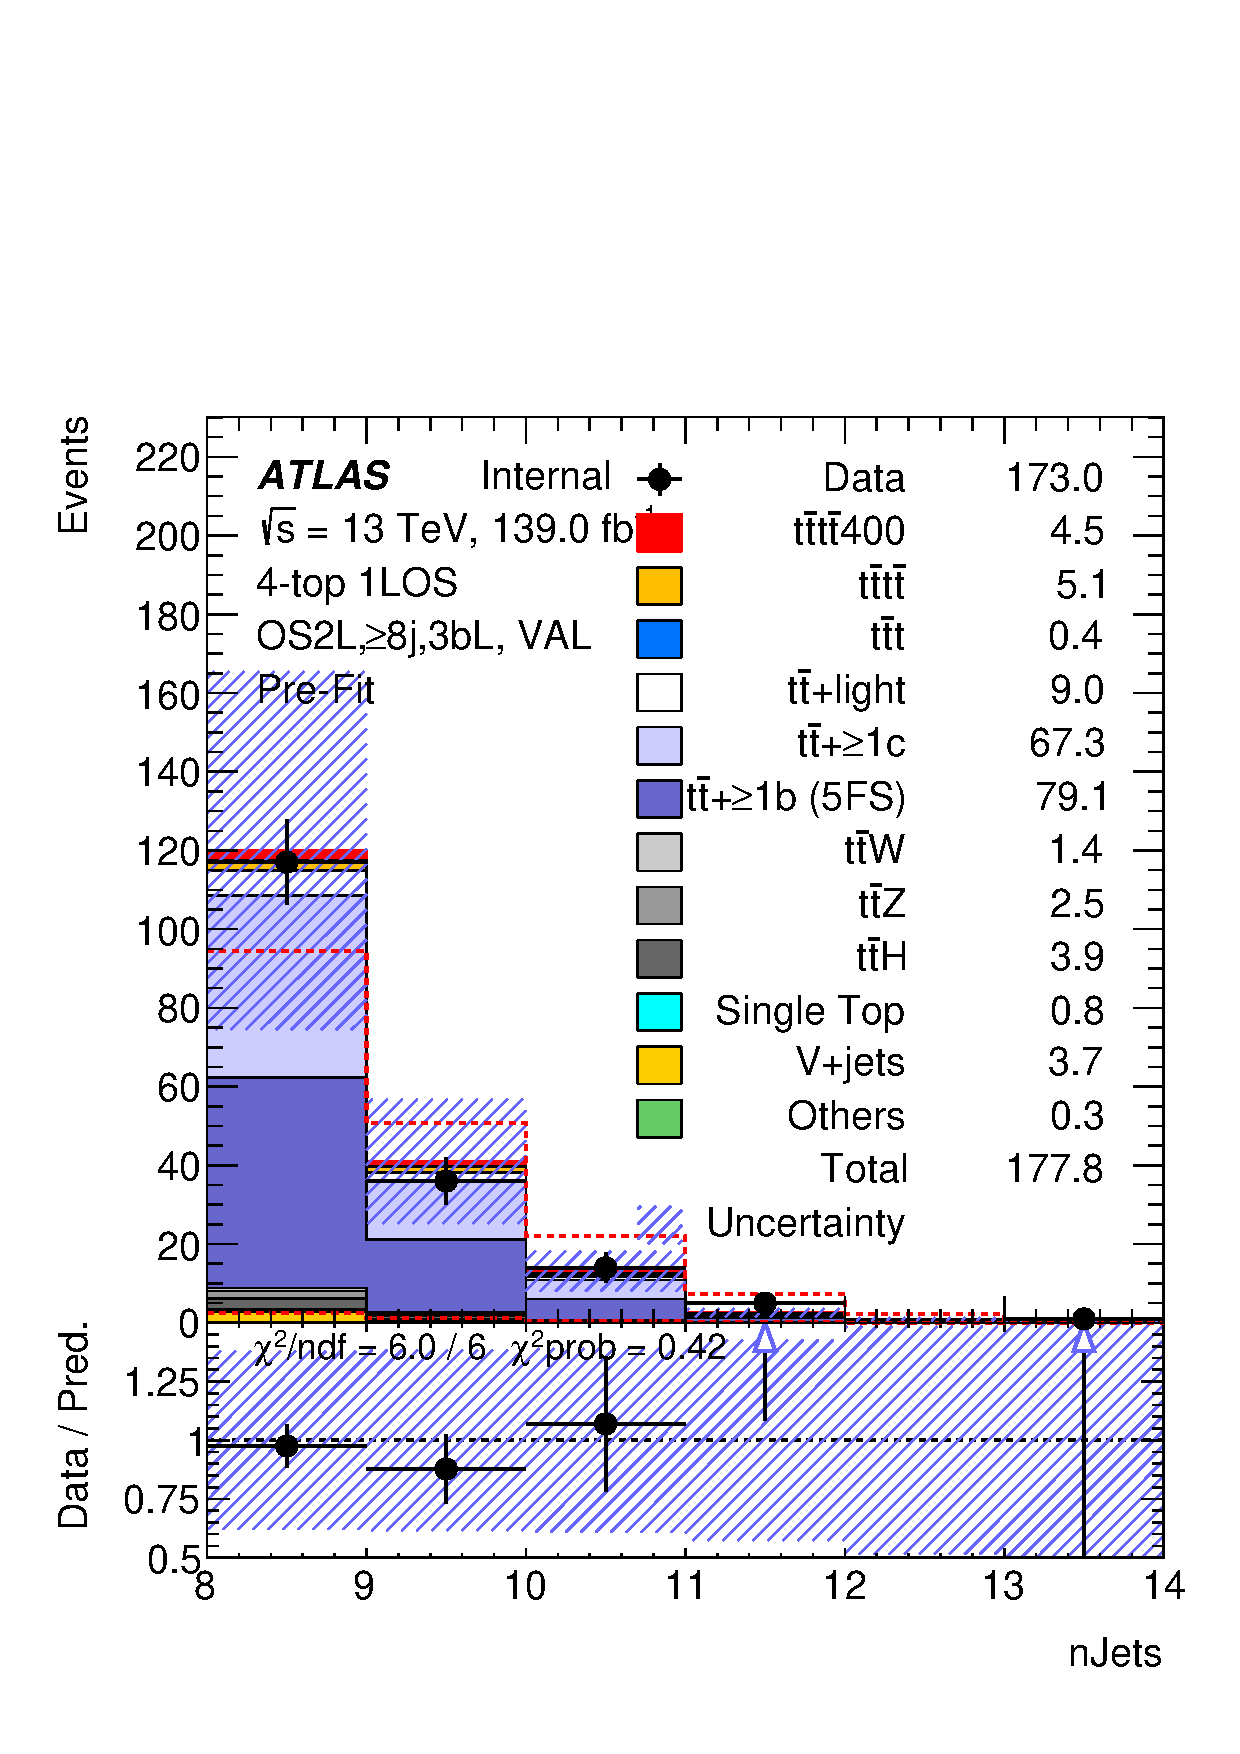
\includegraphics[width=0.23 \textwidth]{figures/fits/GNN/400/all/data_unblindedBonly/Plots/val_os2l_ge8j3bL_nJets.pdf} &
        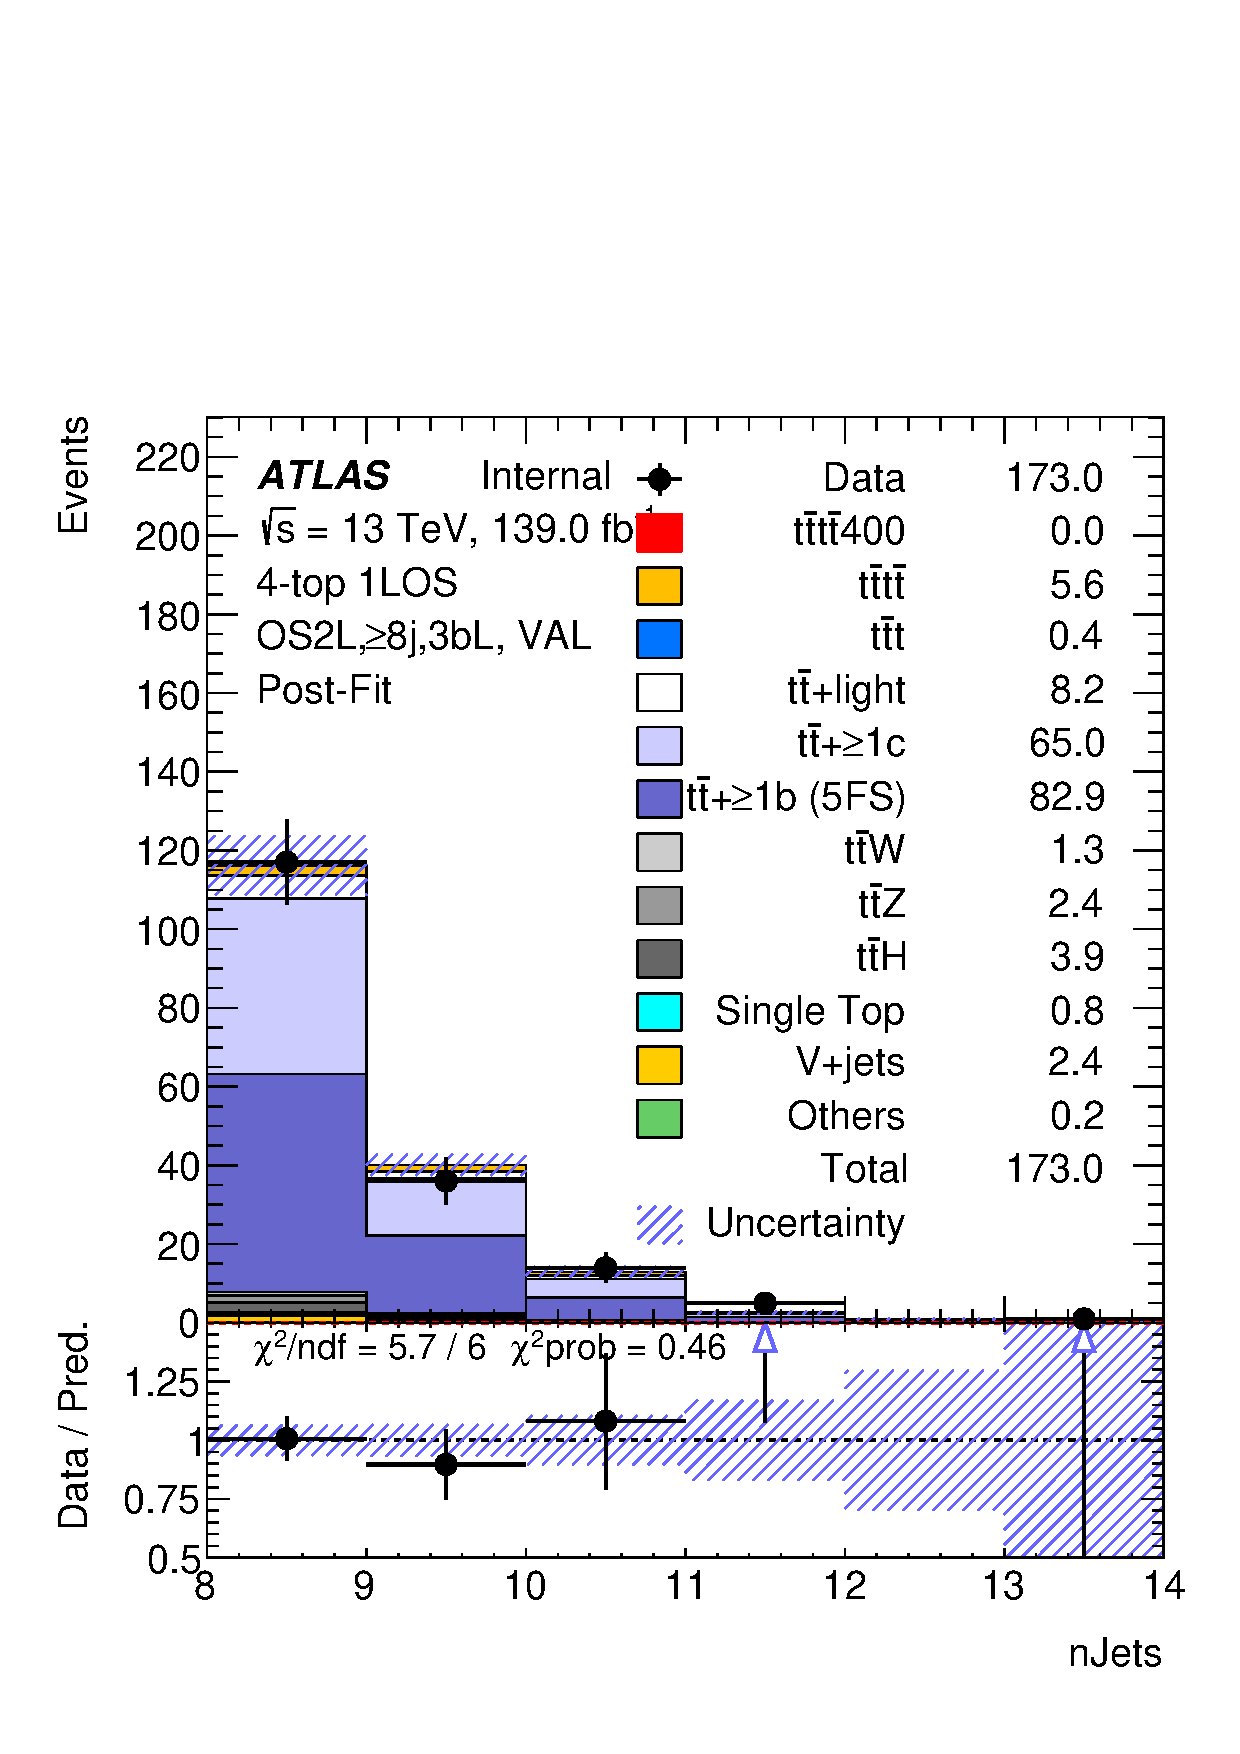
\includegraphics[width=0.23 \textwidth]{figures/fits/GNN/400/all/data_unblindedBonly/Plots/val_os2l_ge8j3bL_nJets_postFit.pdf} &
        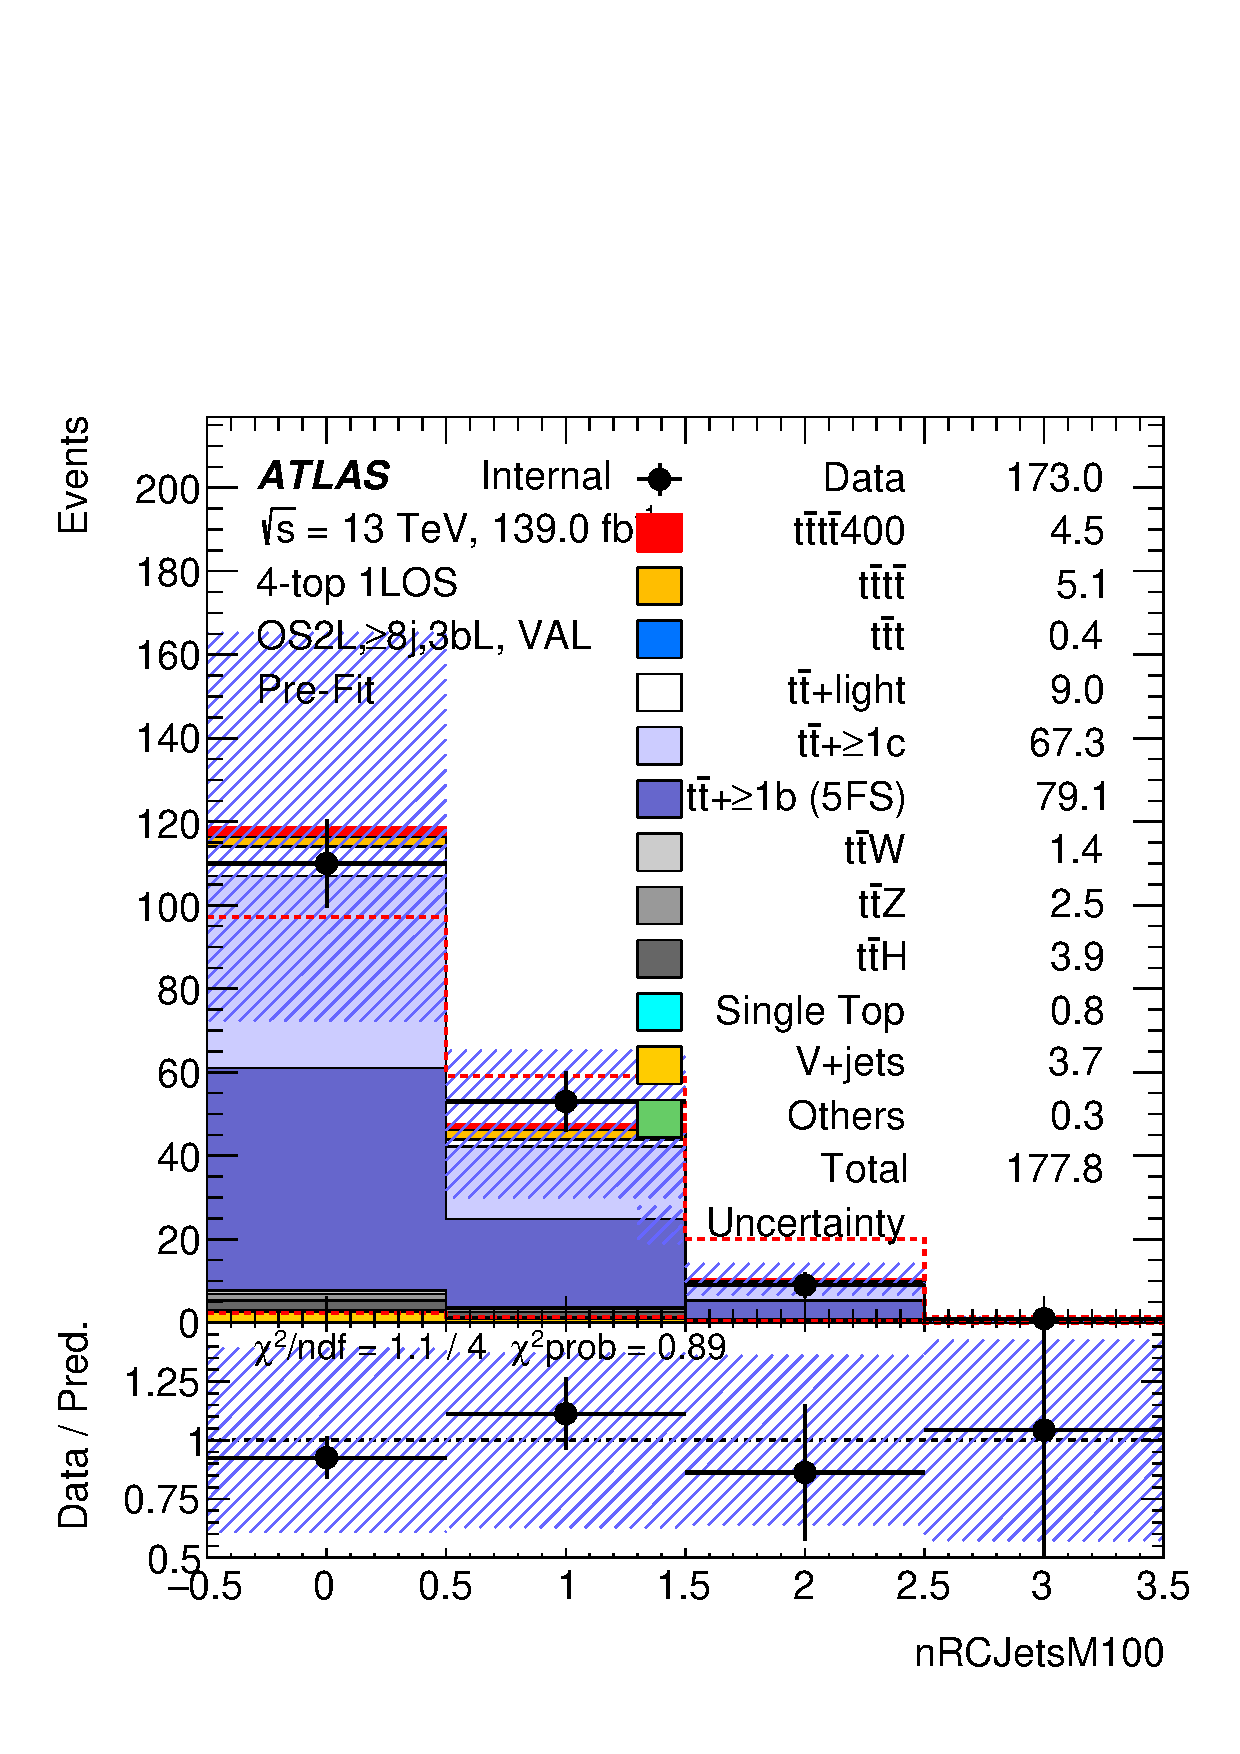
\includegraphics[width=0.23 \textwidth]{figures/fits/GNN/400/all/data_unblindedBonly/Plots/val_os2l_ge8j3bL_nRCJetsM100.pdf} &
        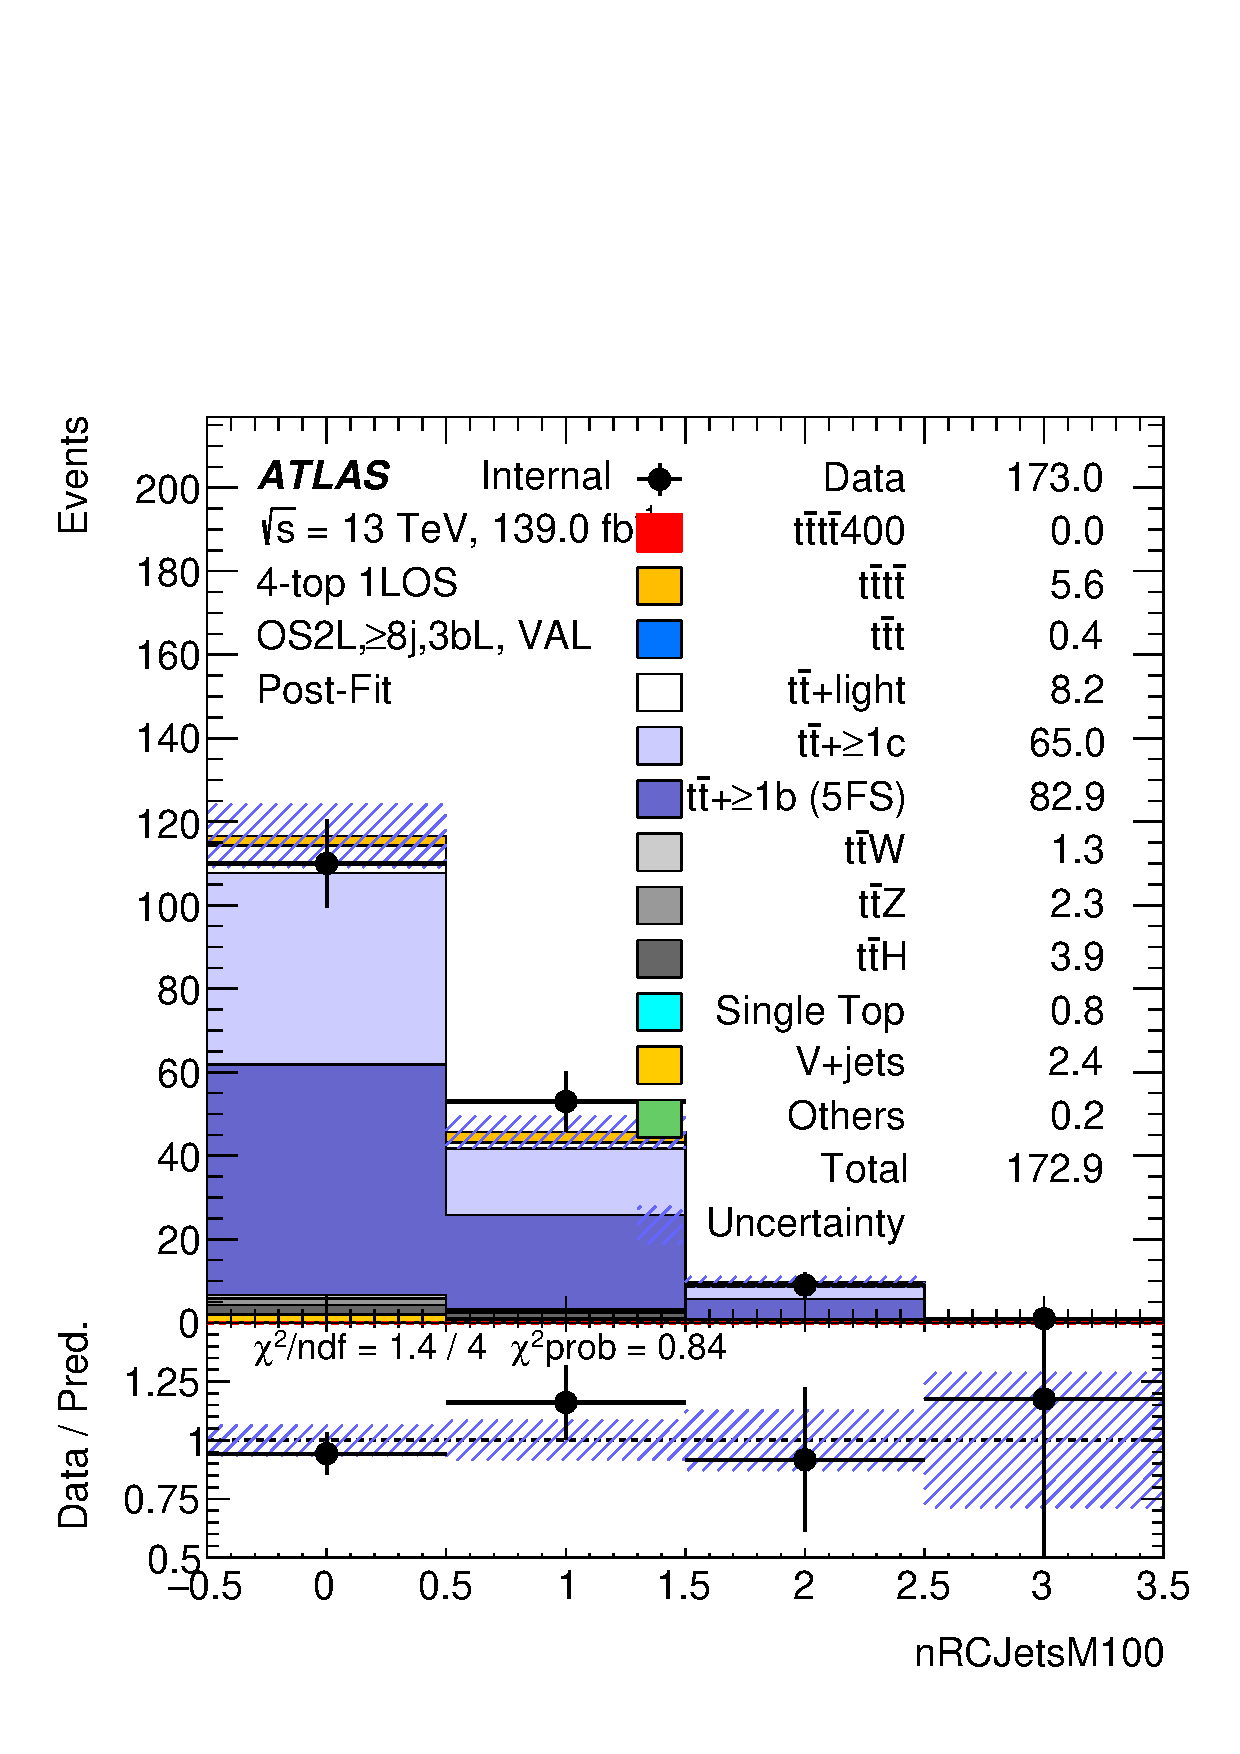
\includegraphics[width=0.23 \textwidth]{figures/fits/GNN/400/all/data_unblindedBonly/Plots/val_os2l_ge8j3bL_nRCJetsM100_postFit.pdf} \\

        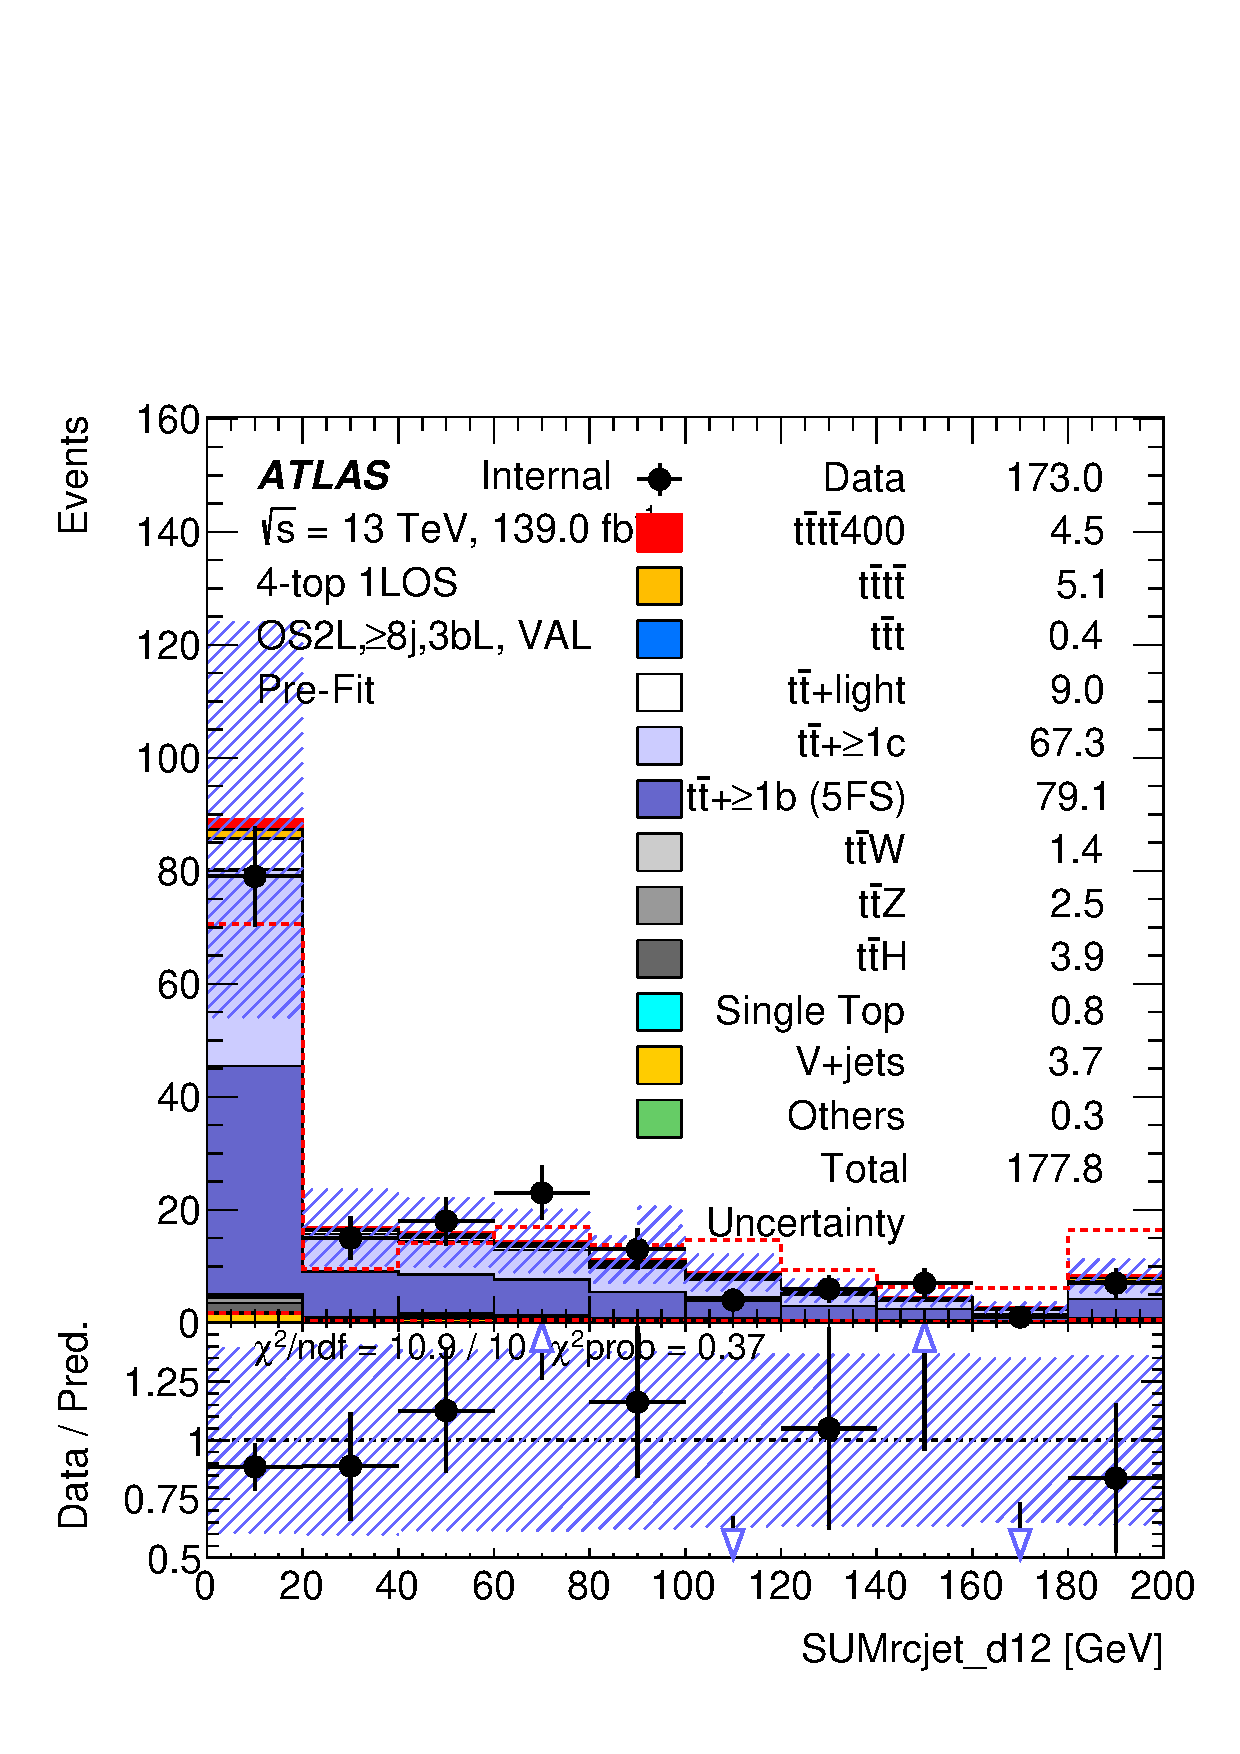
\includegraphics[width=0.23 \textwidth]{figures/fits/GNN/400/all/data_unblindedBonly/Plots/val_os2l_ge8j3bL_sum_rcjet_d12.pdf} &
        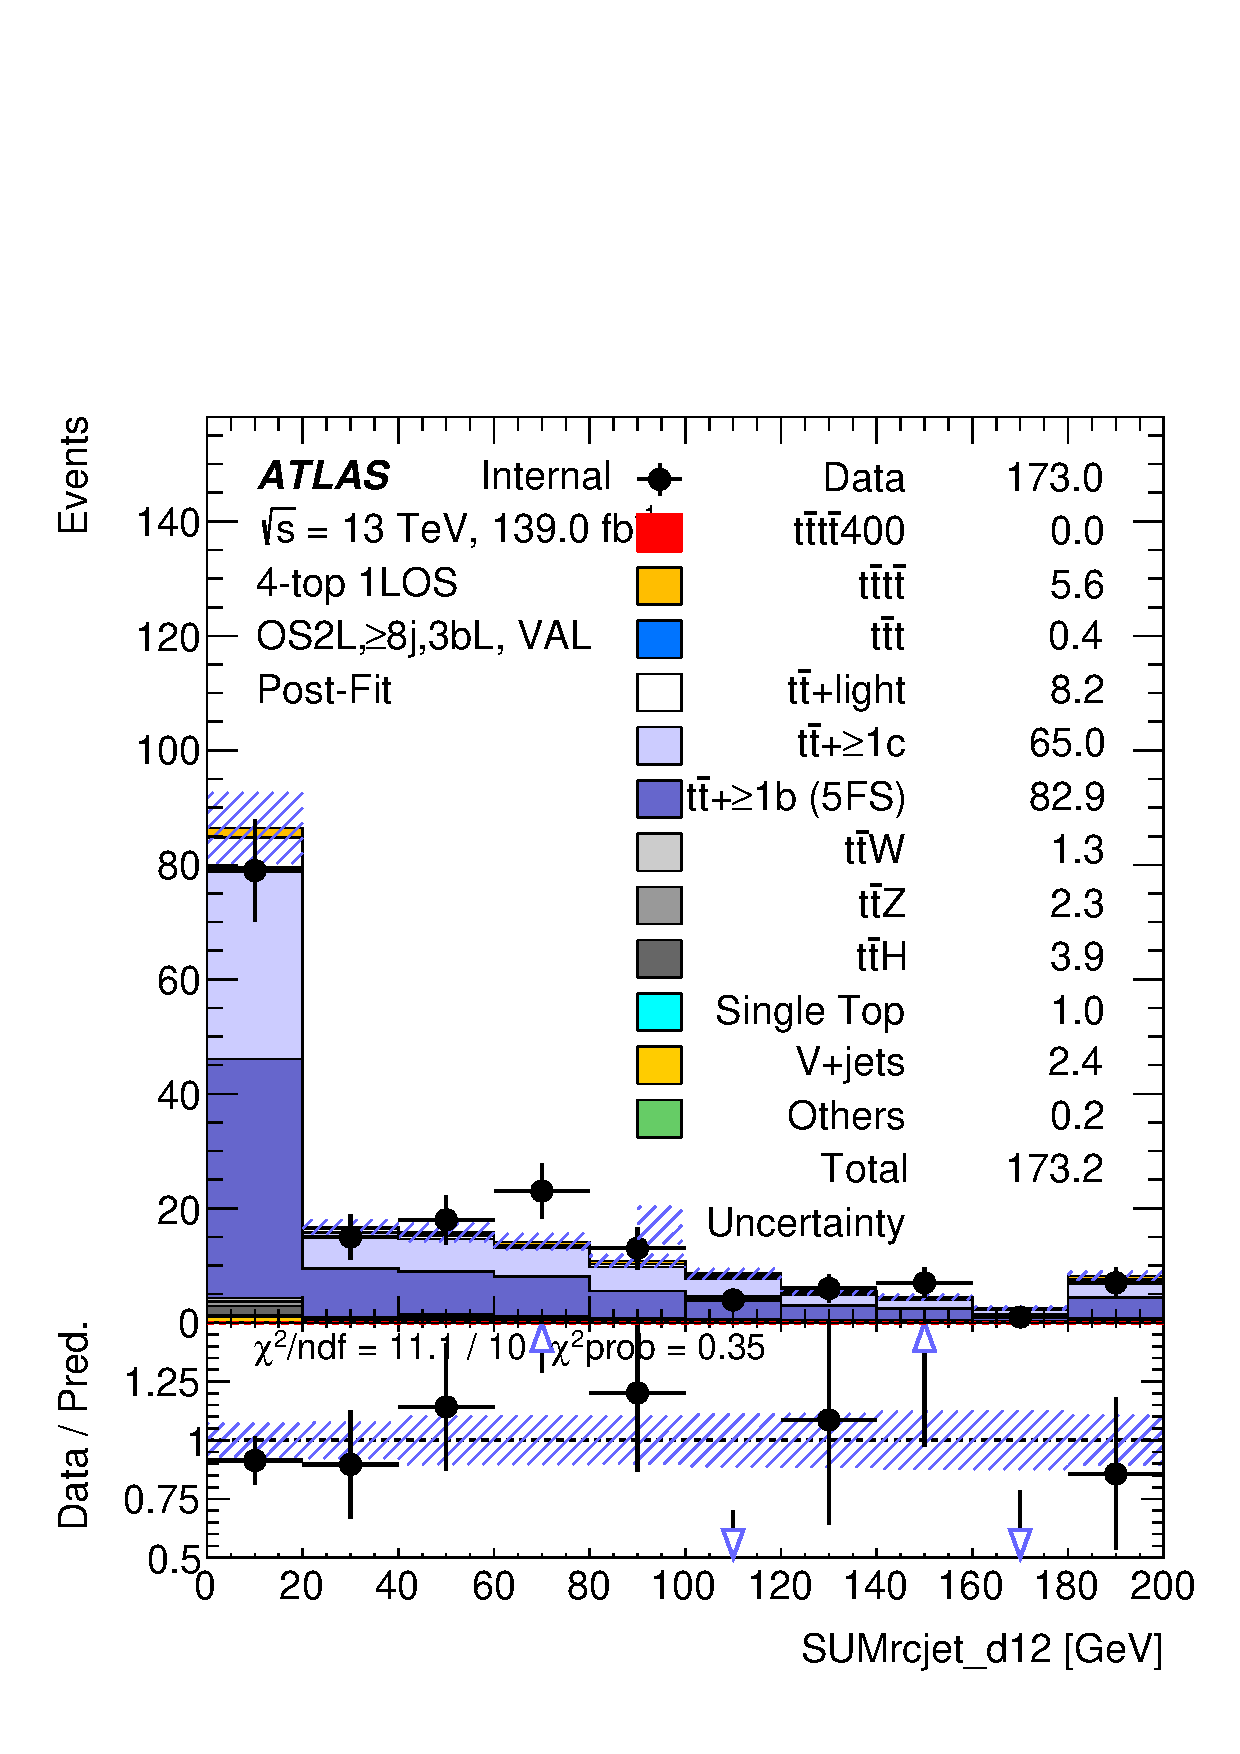
\includegraphics[width=0.23 \textwidth]{figures/fits/GNN/400/all/data_unblindedBonly/Plots/val_os2l_ge8j3bL_sum_rcjet_d12_postFit.pdf} &
        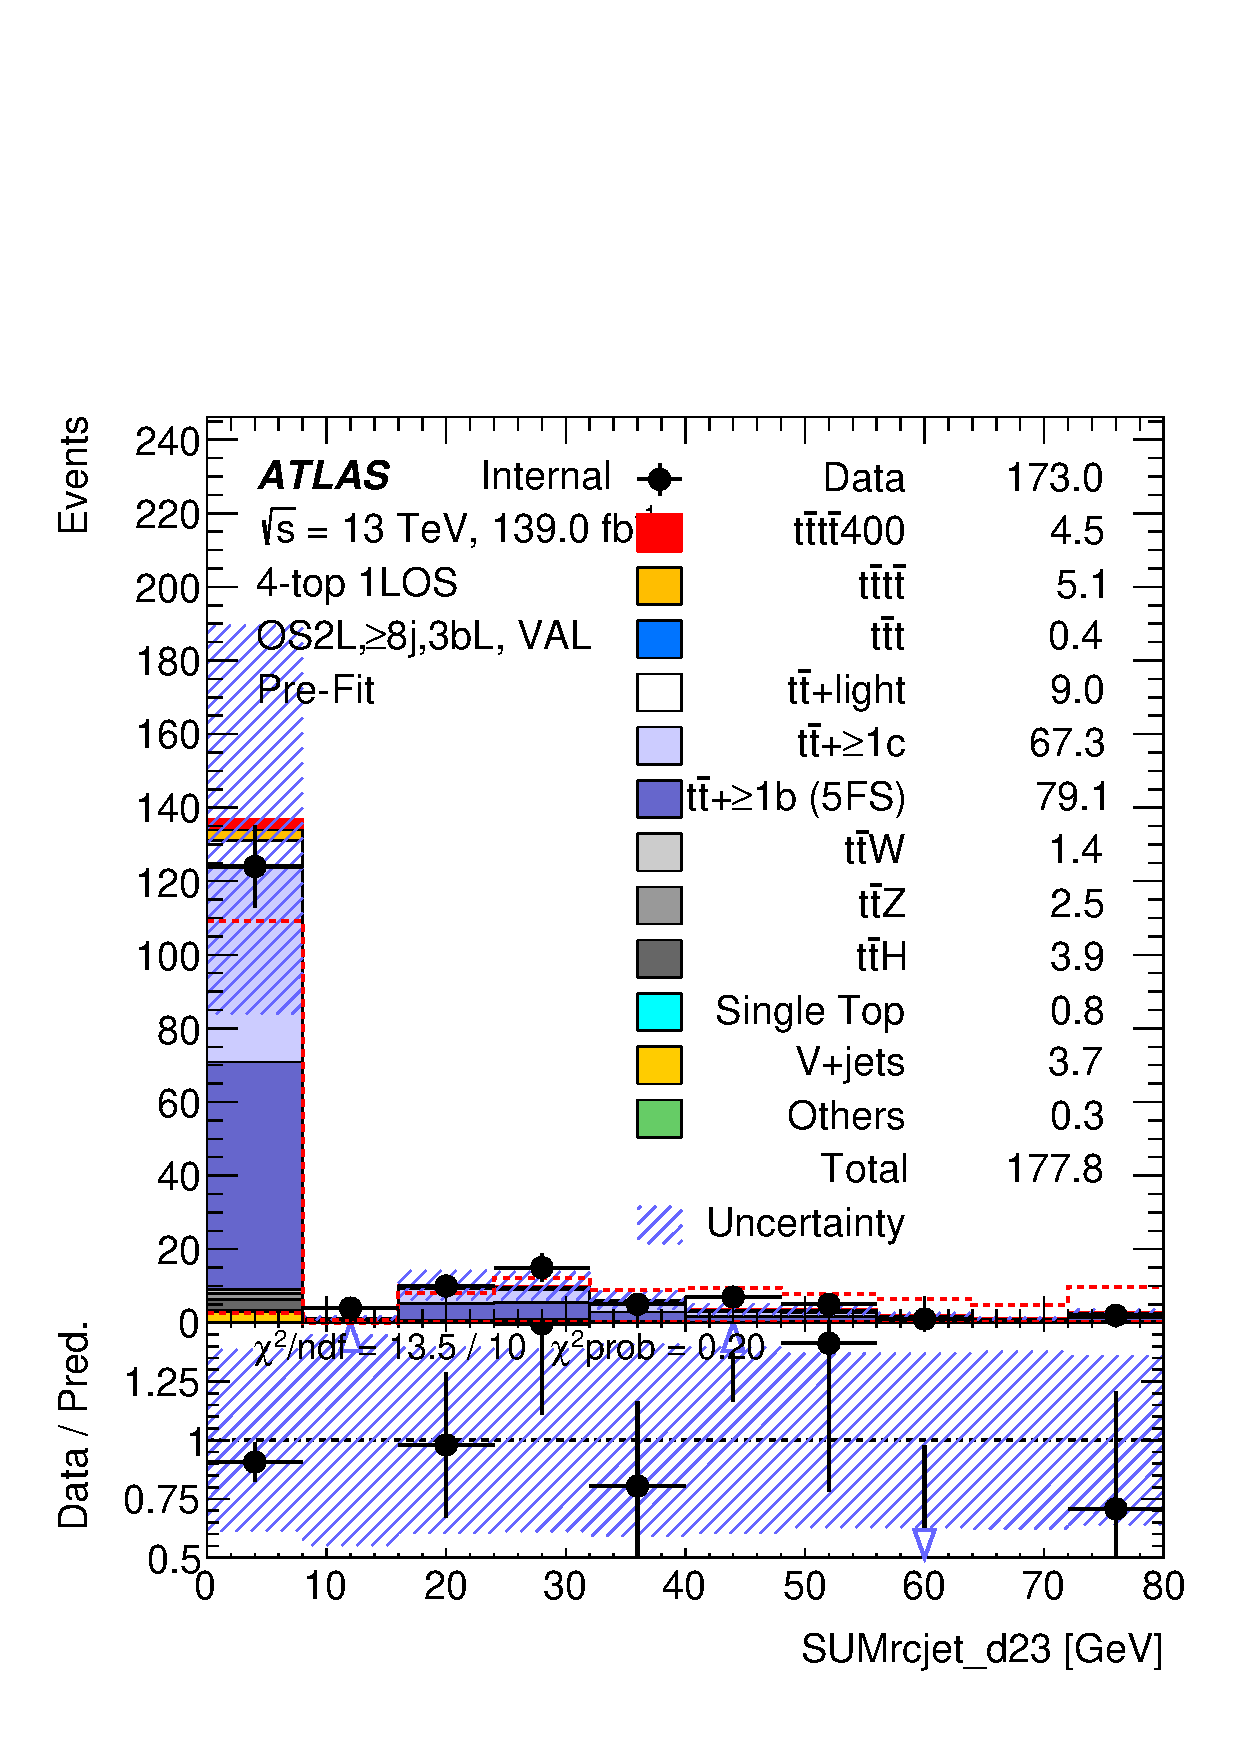
\includegraphics[width=0.23 \textwidth]{figures/fits/GNN/400/all/data_unblindedBonly/Plots/val_os2l_ge8j3bL_sum_rcjet_d23.pdf} &
        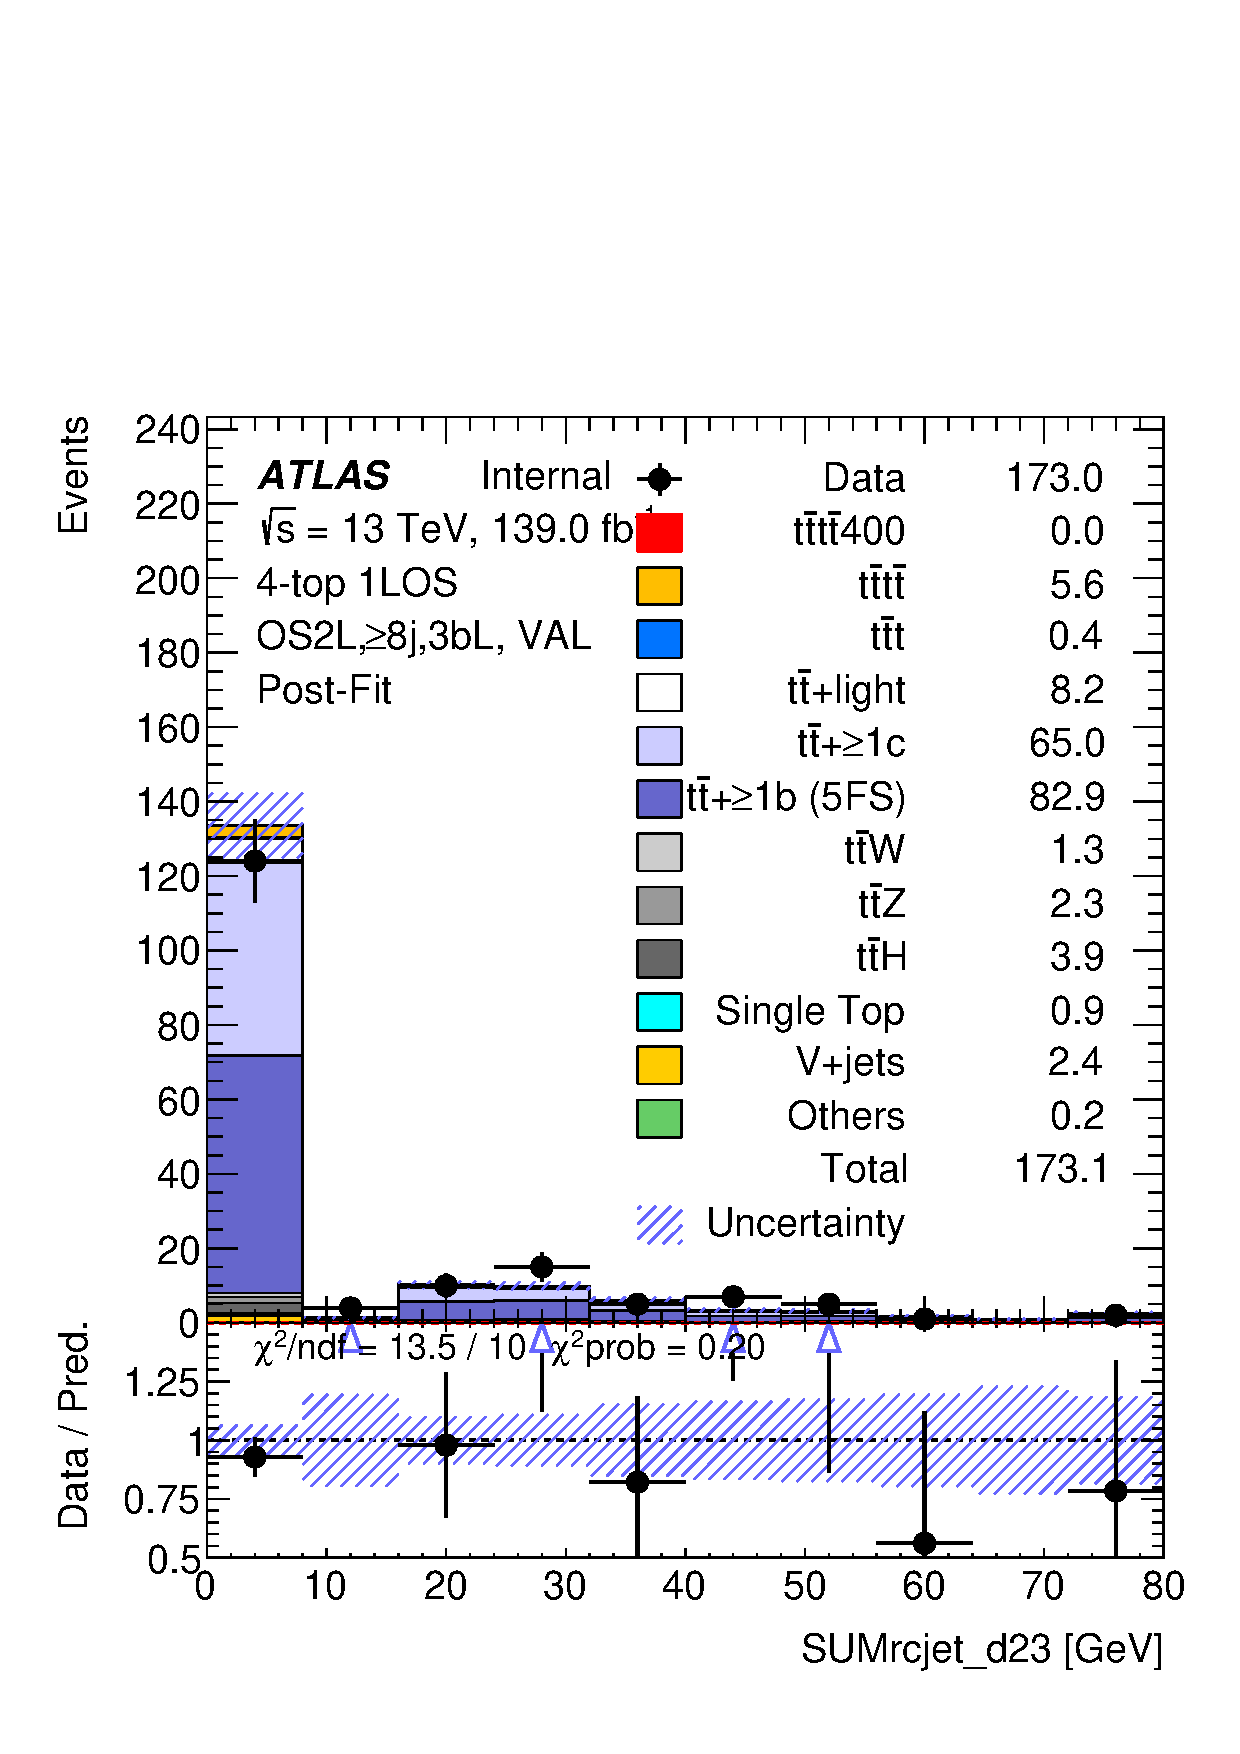
\includegraphics[width=0.23 \textwidth]{figures/fits/GNN/400/all/data_unblindedBonly/Plots/val_os2l_ge8j3bL_sum_rcjet_d23_postFit.pdf} \\

        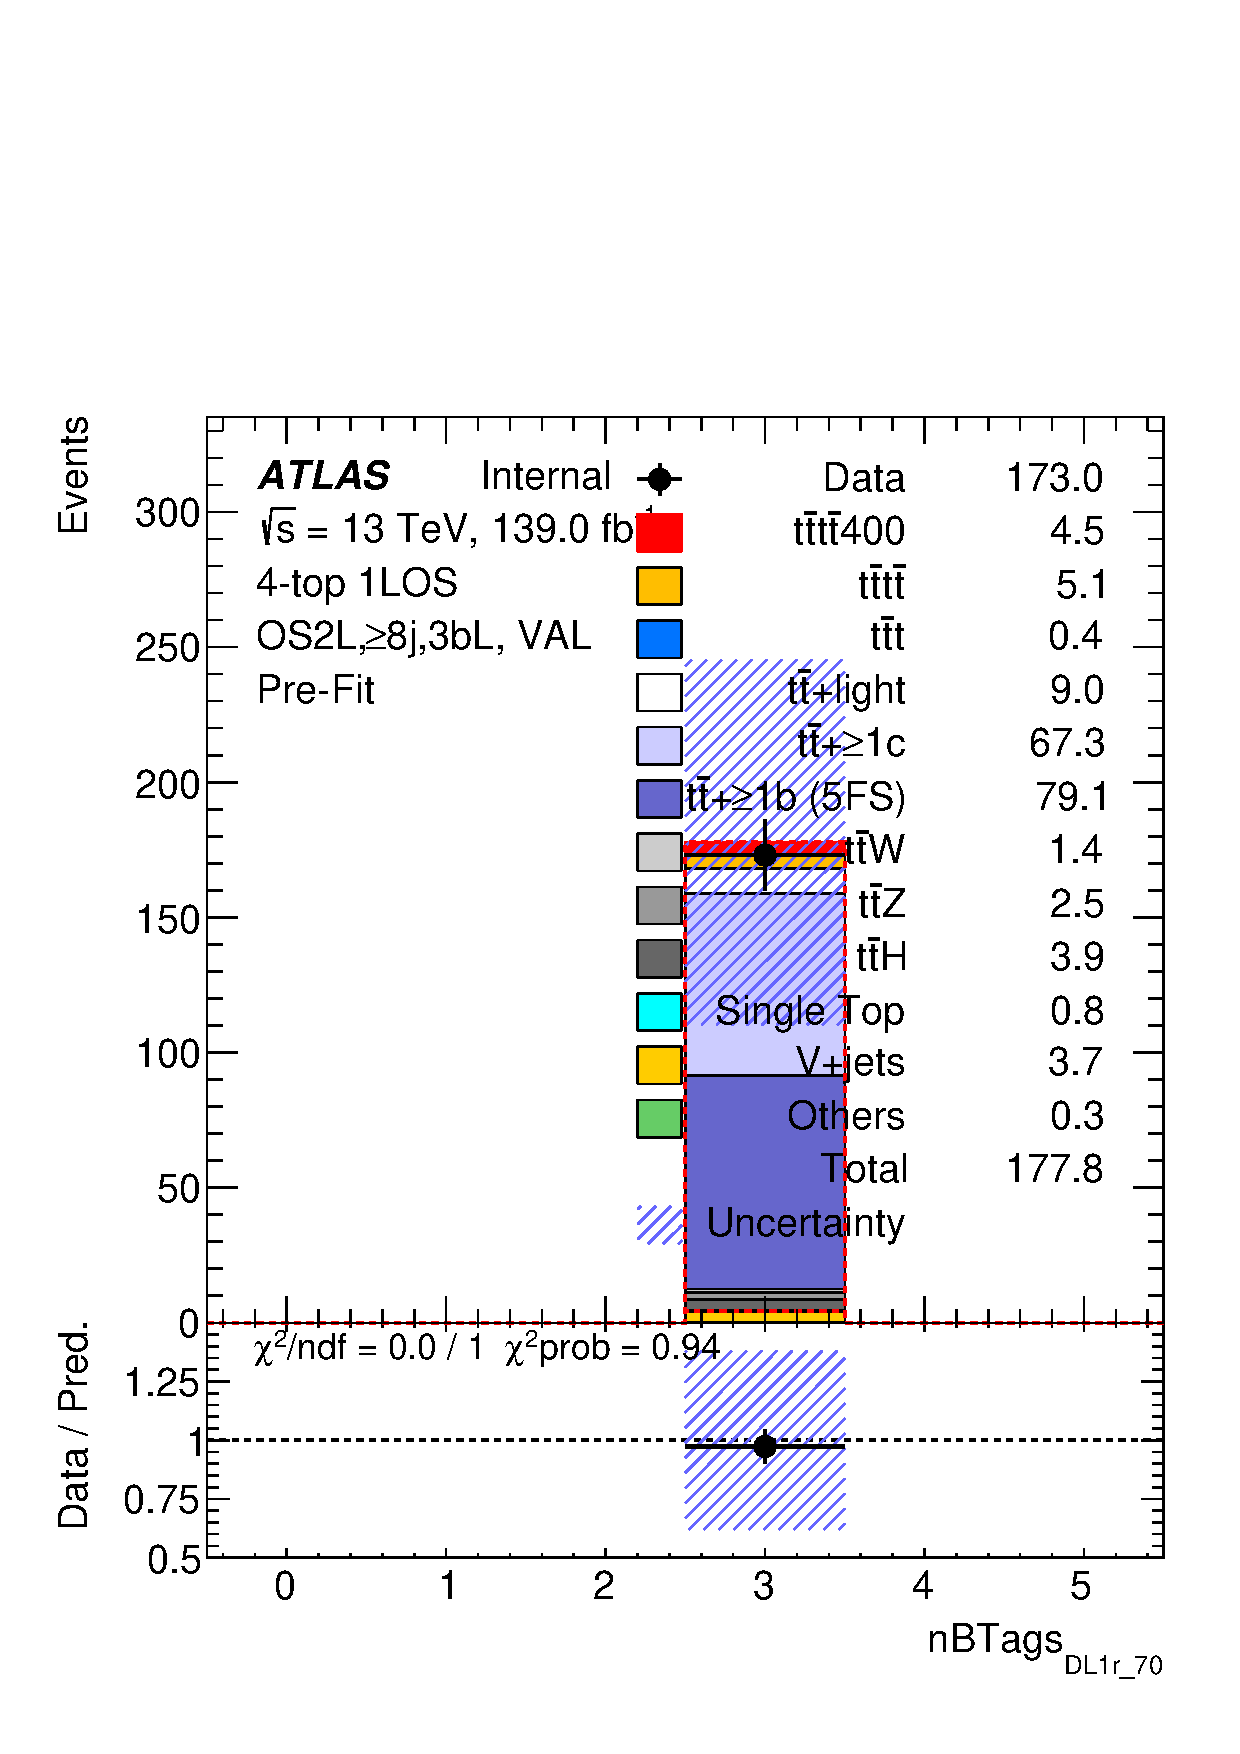
\includegraphics[width=0.23 \textwidth]{figures/fits/GNN/400/all/data_unblindedBonly/Plots/val_os2l_ge8j3bL_nBTags_DL1r_70.pdf} &
        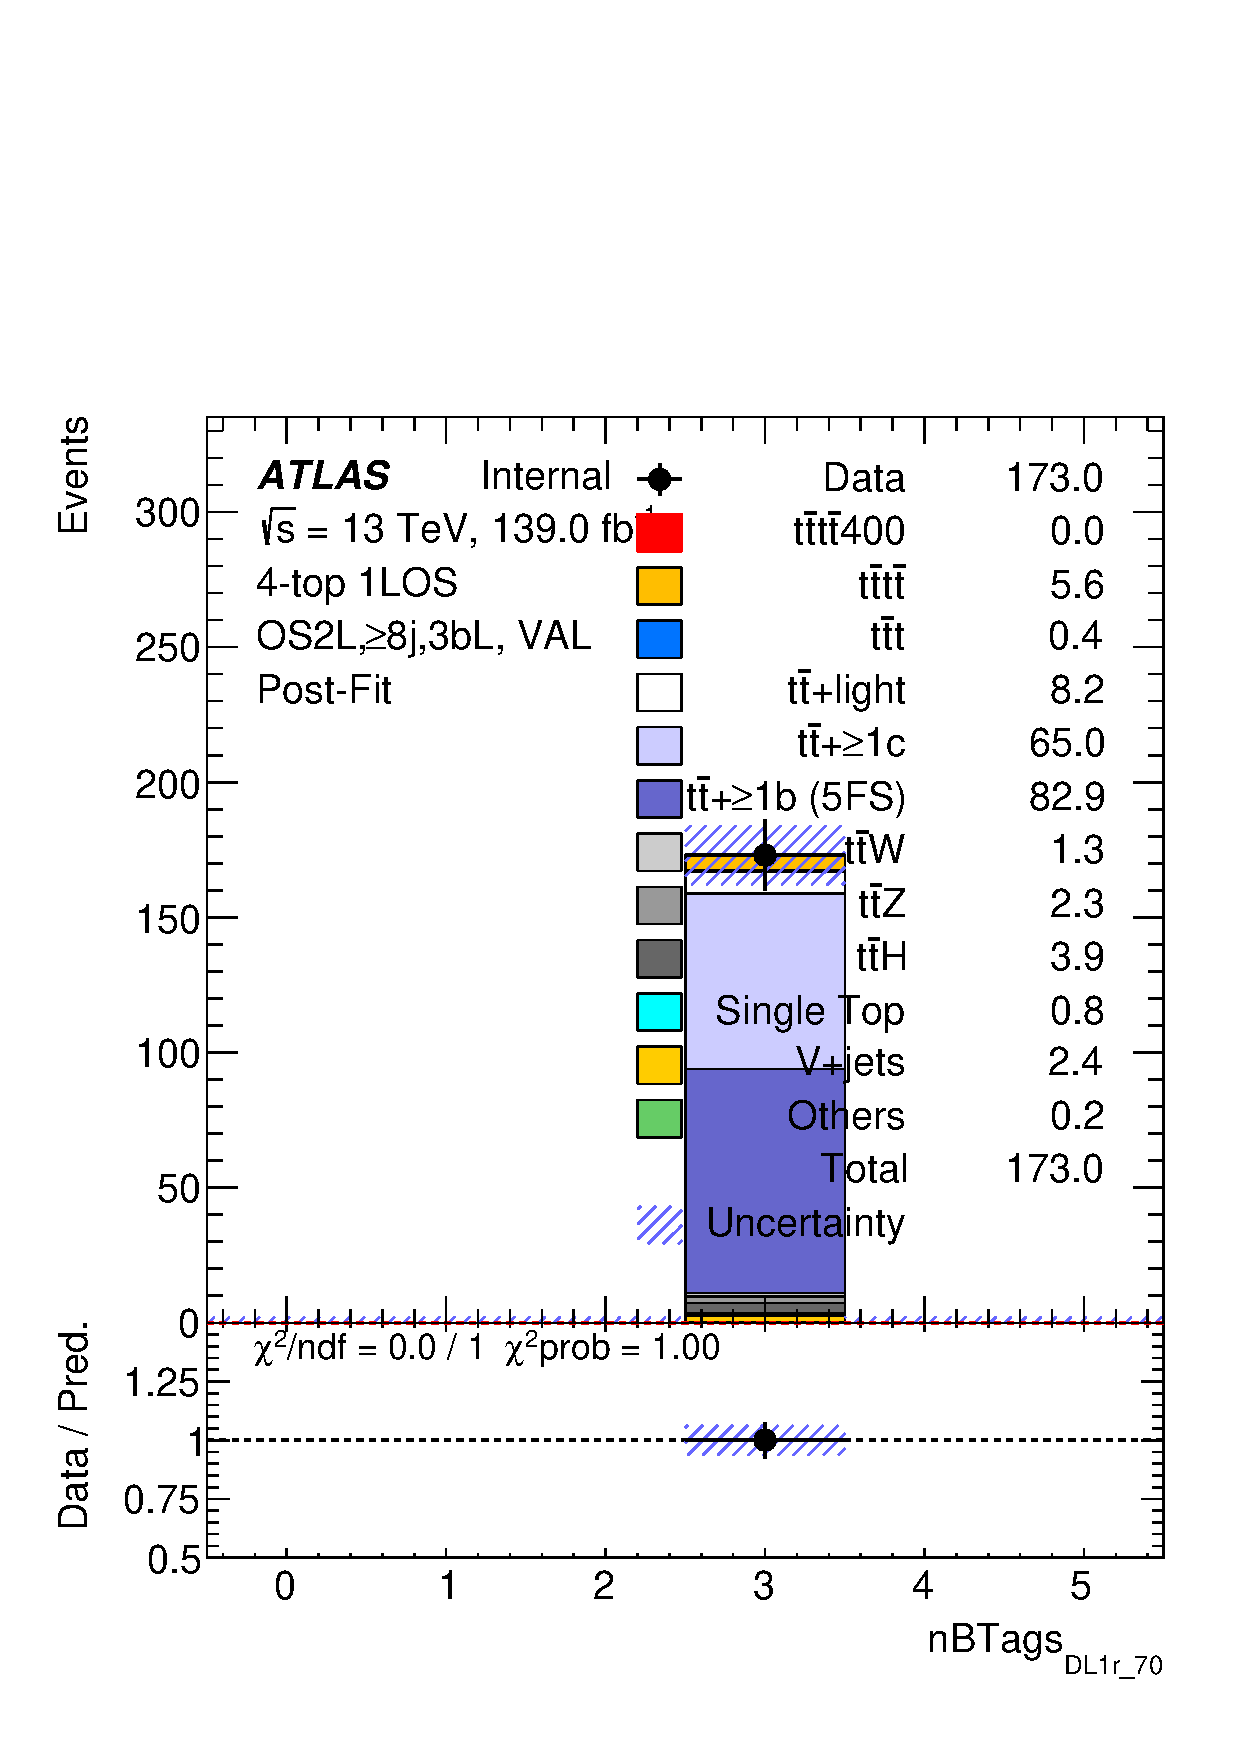
\includegraphics[width=0.23 \textwidth]{figures/fits/GNN/400/all/data_unblindedBonly/Plots/val_os2l_ge8j3bL_nBTags_DL1r_70_postFit.pdf} &
        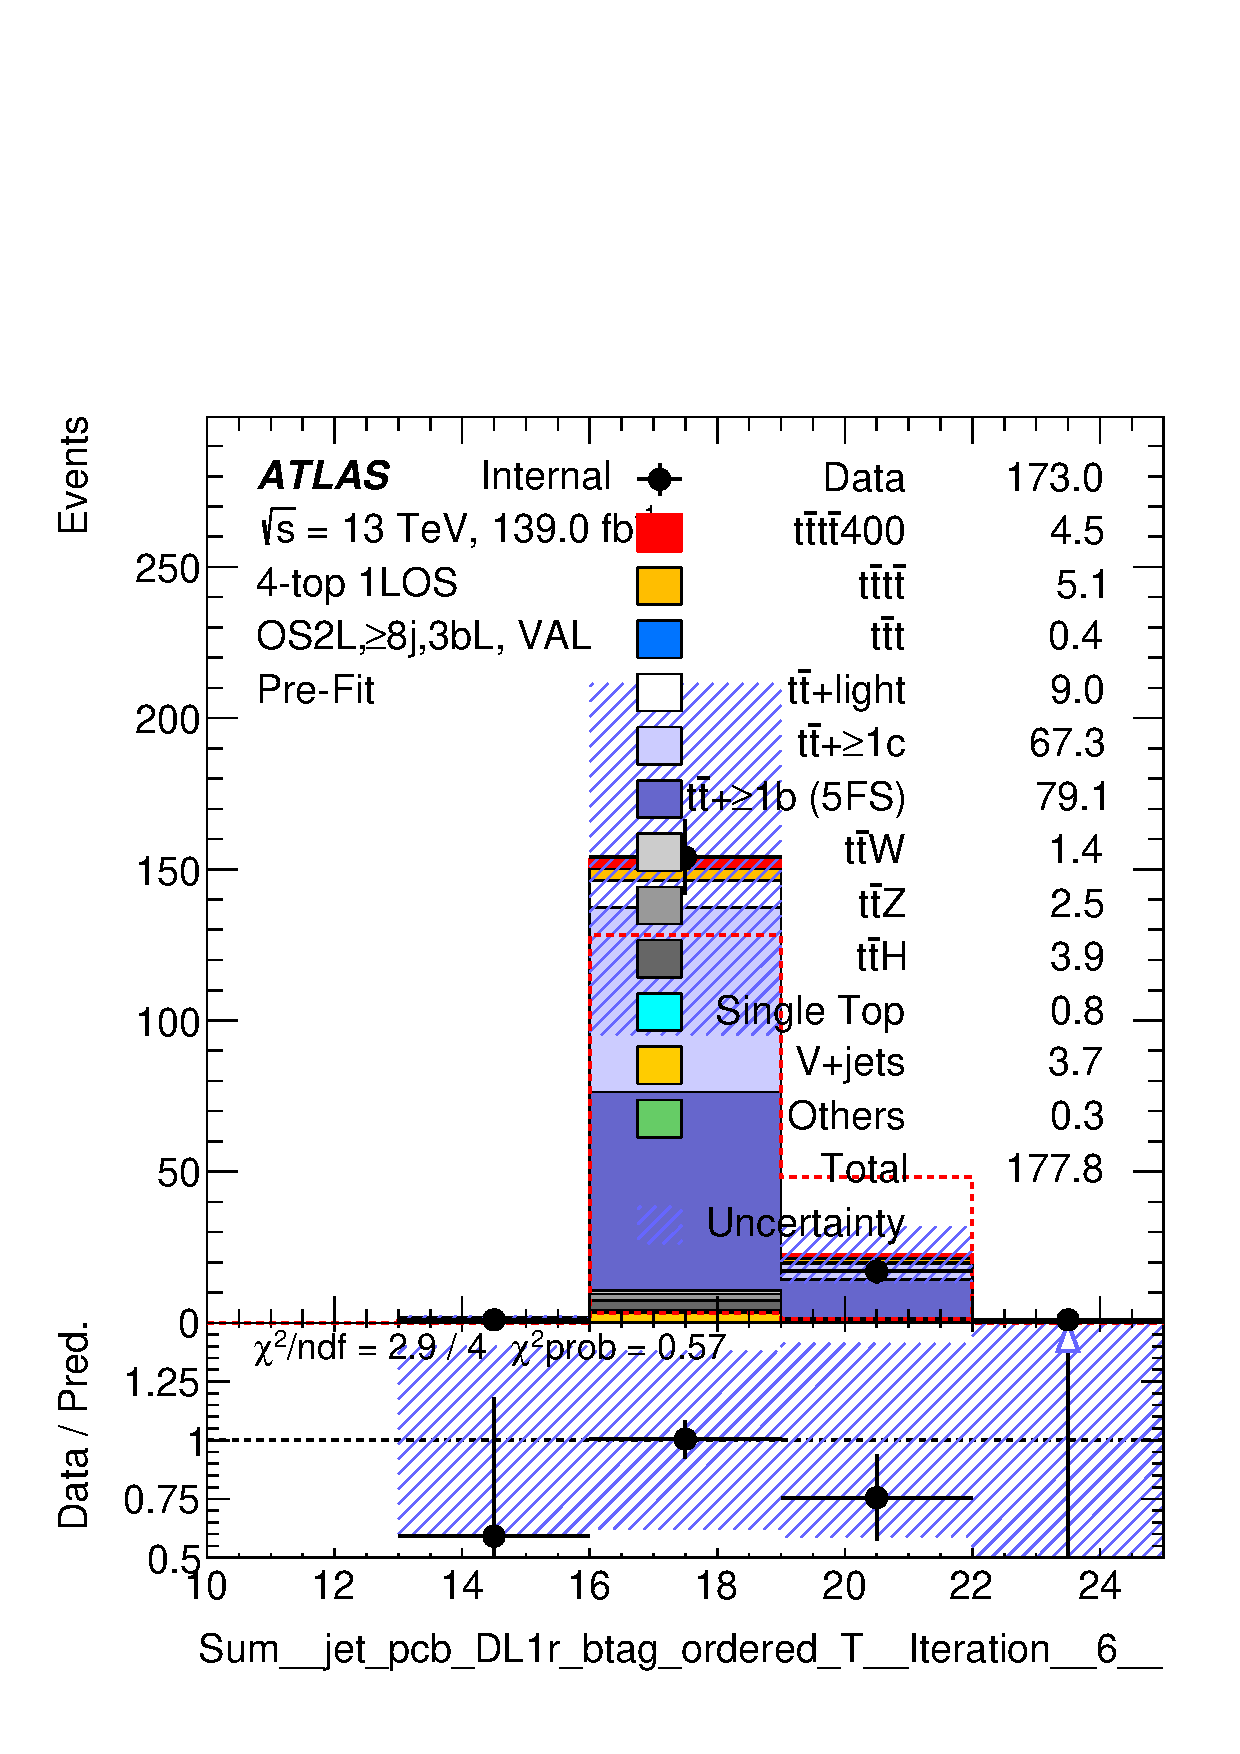
\includegraphics[width=0.23 \textwidth]{figures/fits/GNN/400/all/data_unblindedBonly/Plots/val_os2l_ge8j3bL_sum_pcb.pdf} &
        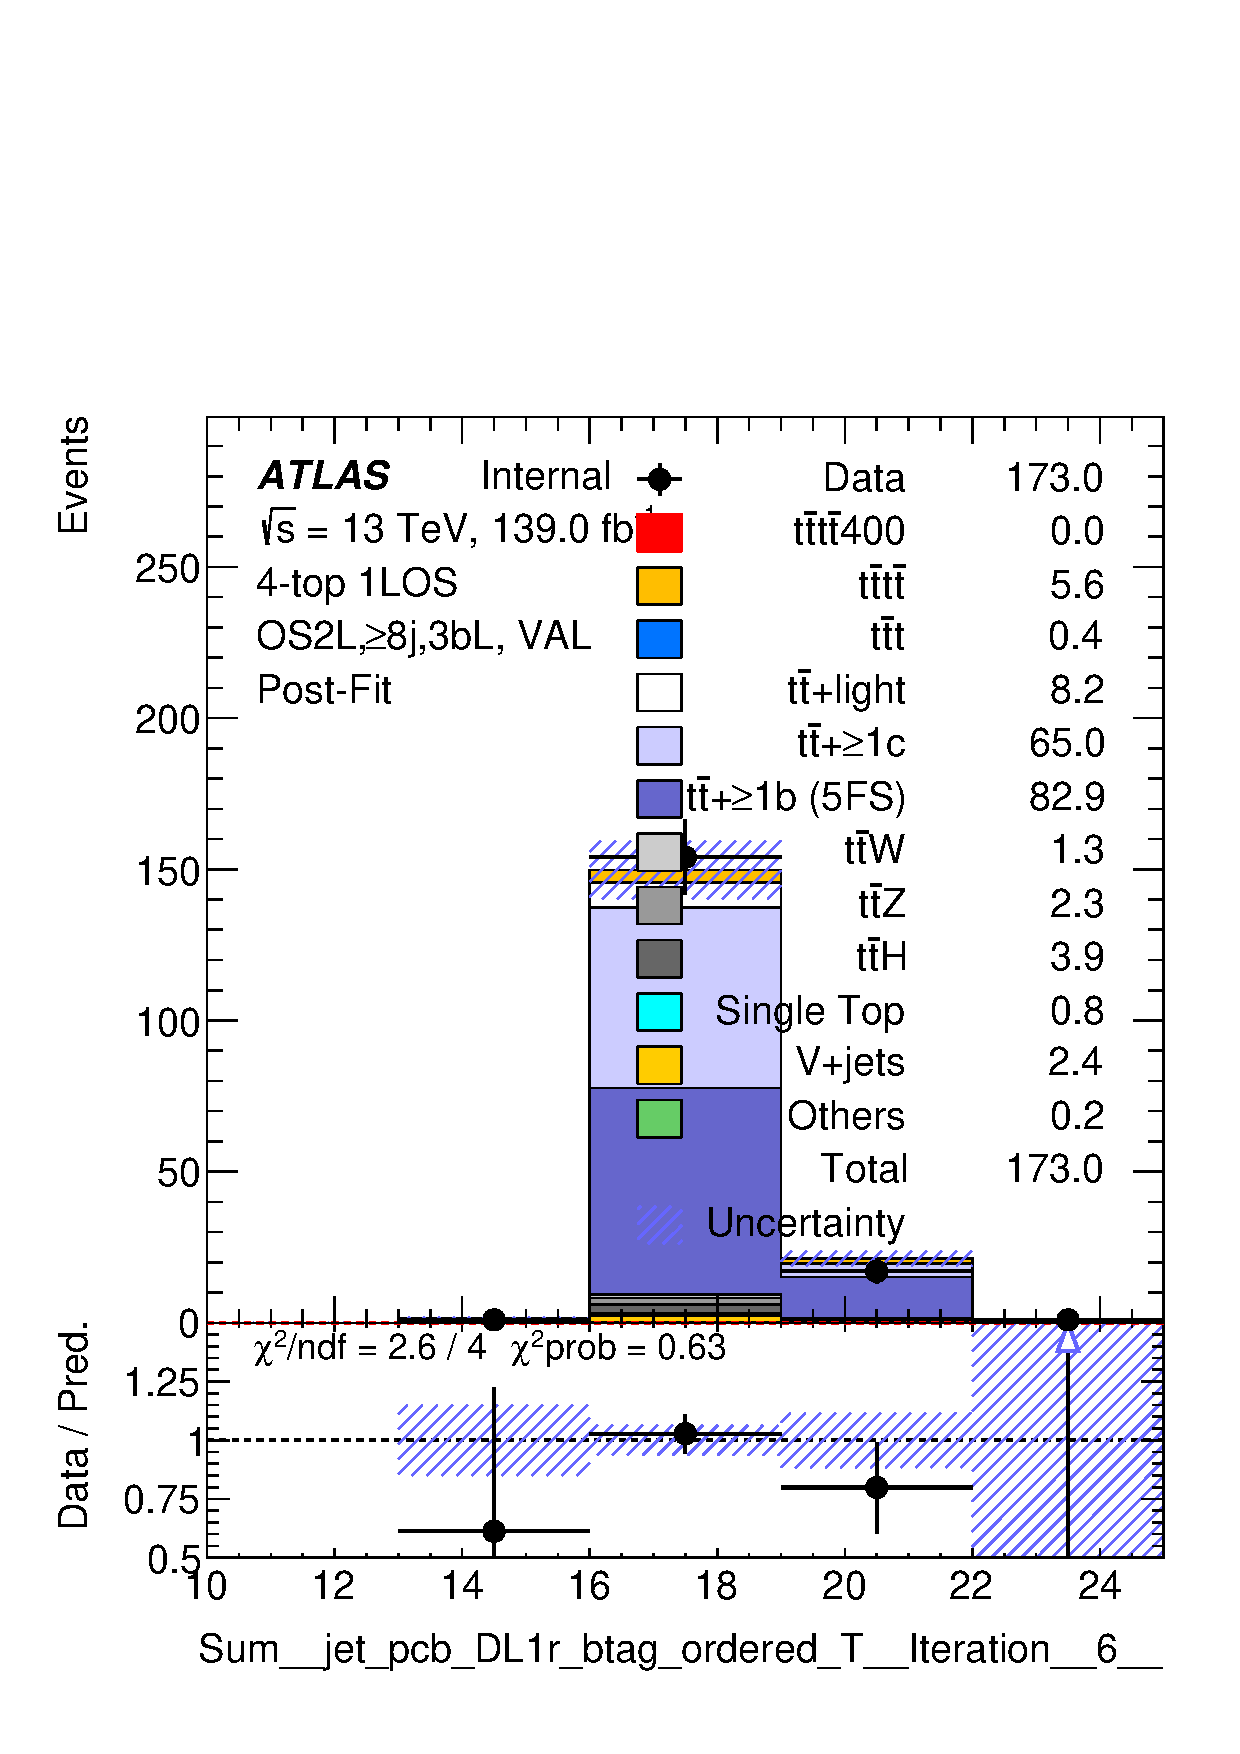
\includegraphics[width=0.23 \textwidth]{figures/fits/GNN/400/all/data_unblindedBonly/Plots/val_os2l_ge8j3bL_sum_pcb_postFit.pdf} \\

        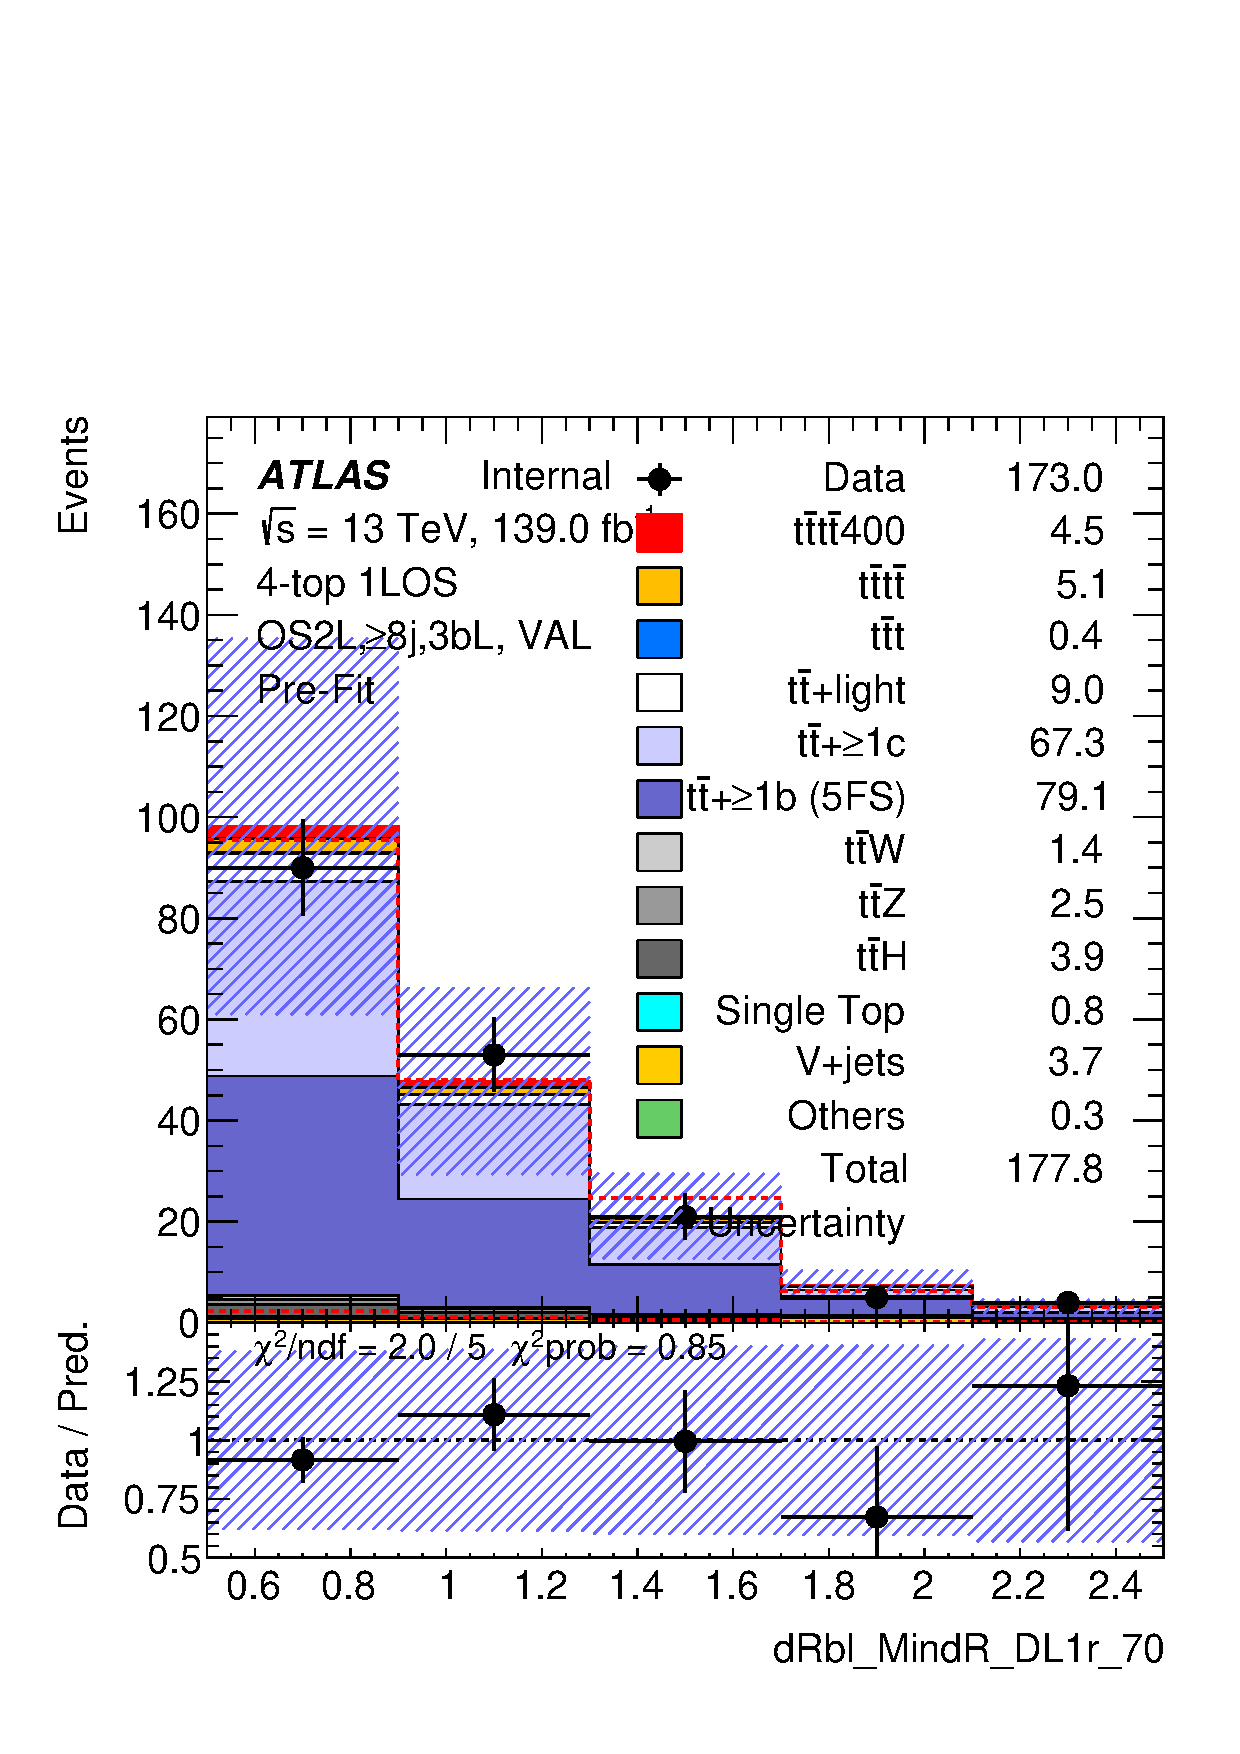
\includegraphics[width=0.23 \textwidth]{figures/fits/GNN/400/all/data_unblindedBonly/Plots/val_os2l_ge8j3bL_dRbl_MindR_DL1r_70.pdf} &
        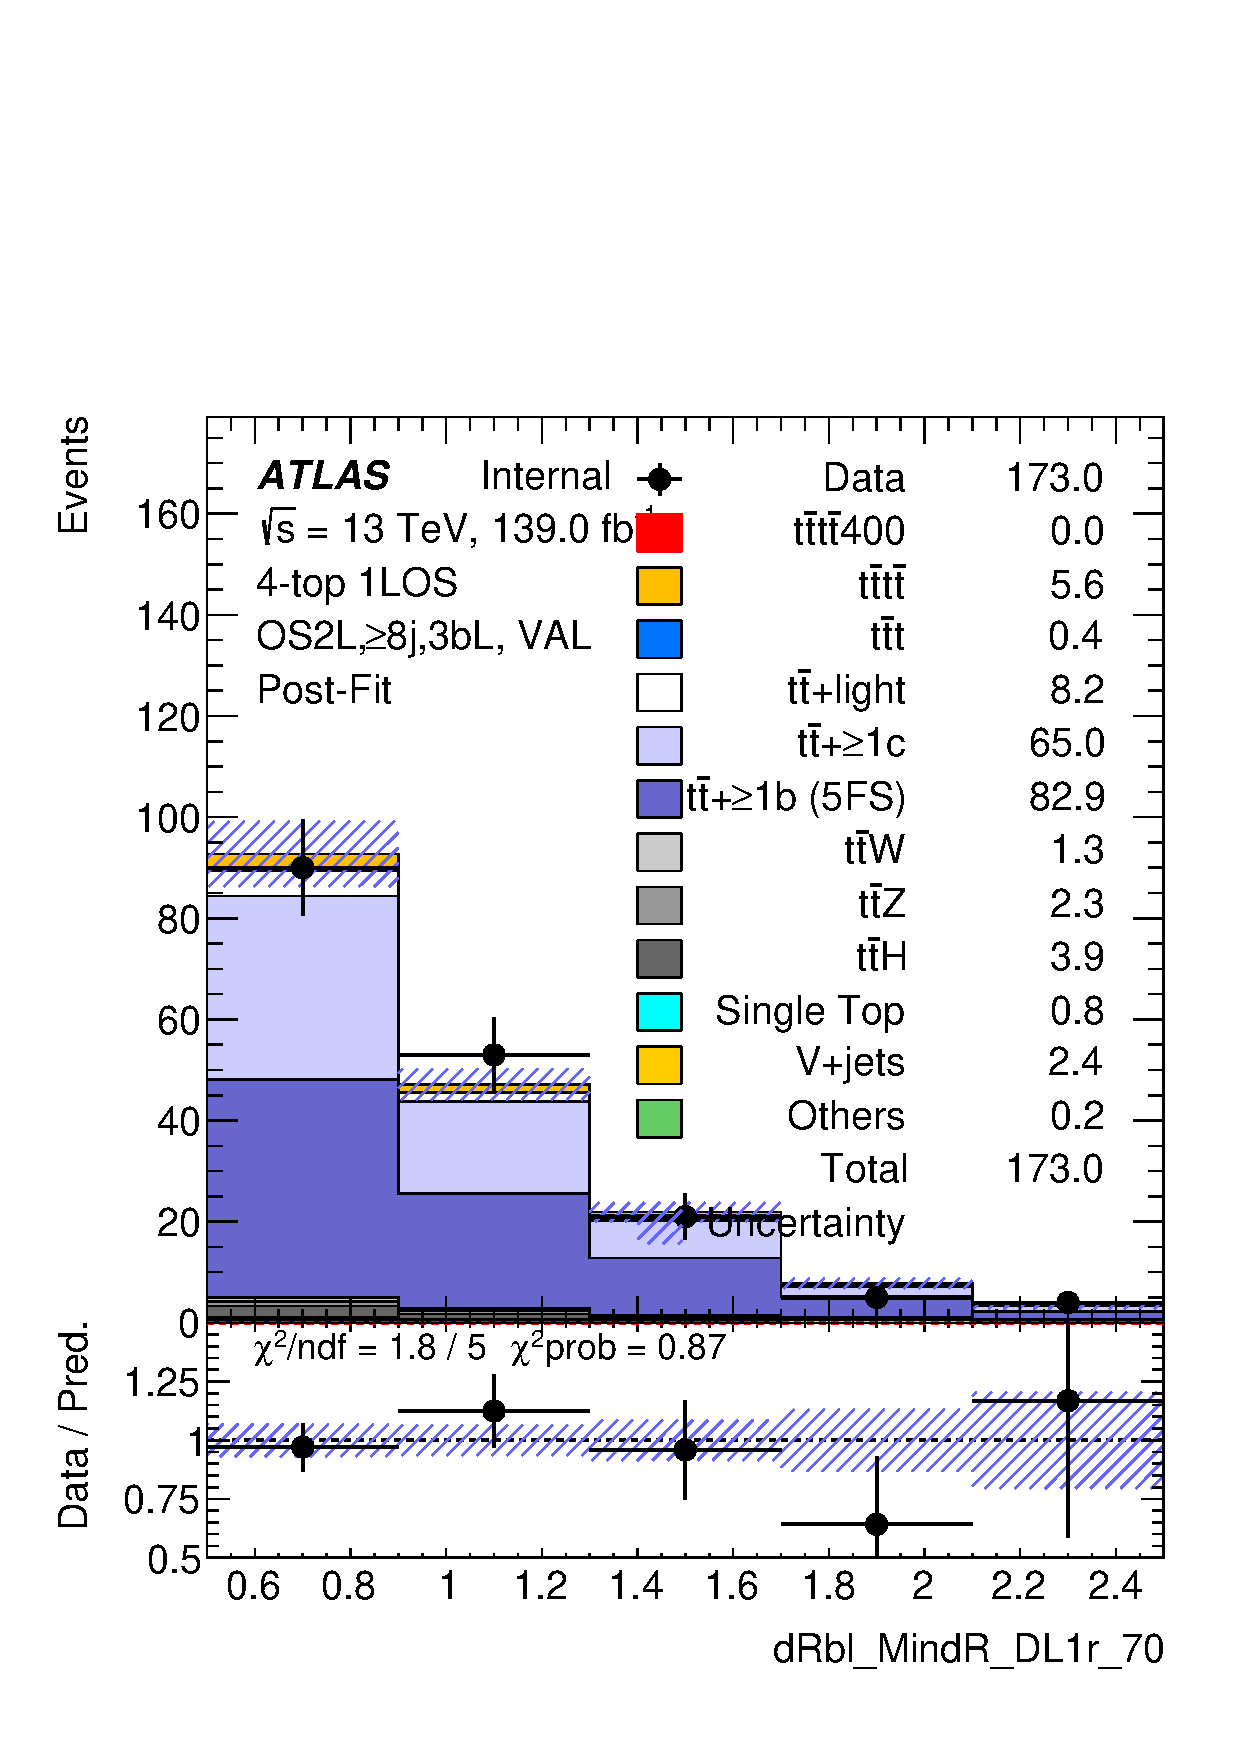
\includegraphics[width=0.23 \textwidth]{figures/fits/GNN/400/all/data_unblindedBonly/Plots/val_os2l_ge8j3bL_dRbl_MindR_DL1r_70_postFit.pdf} &
        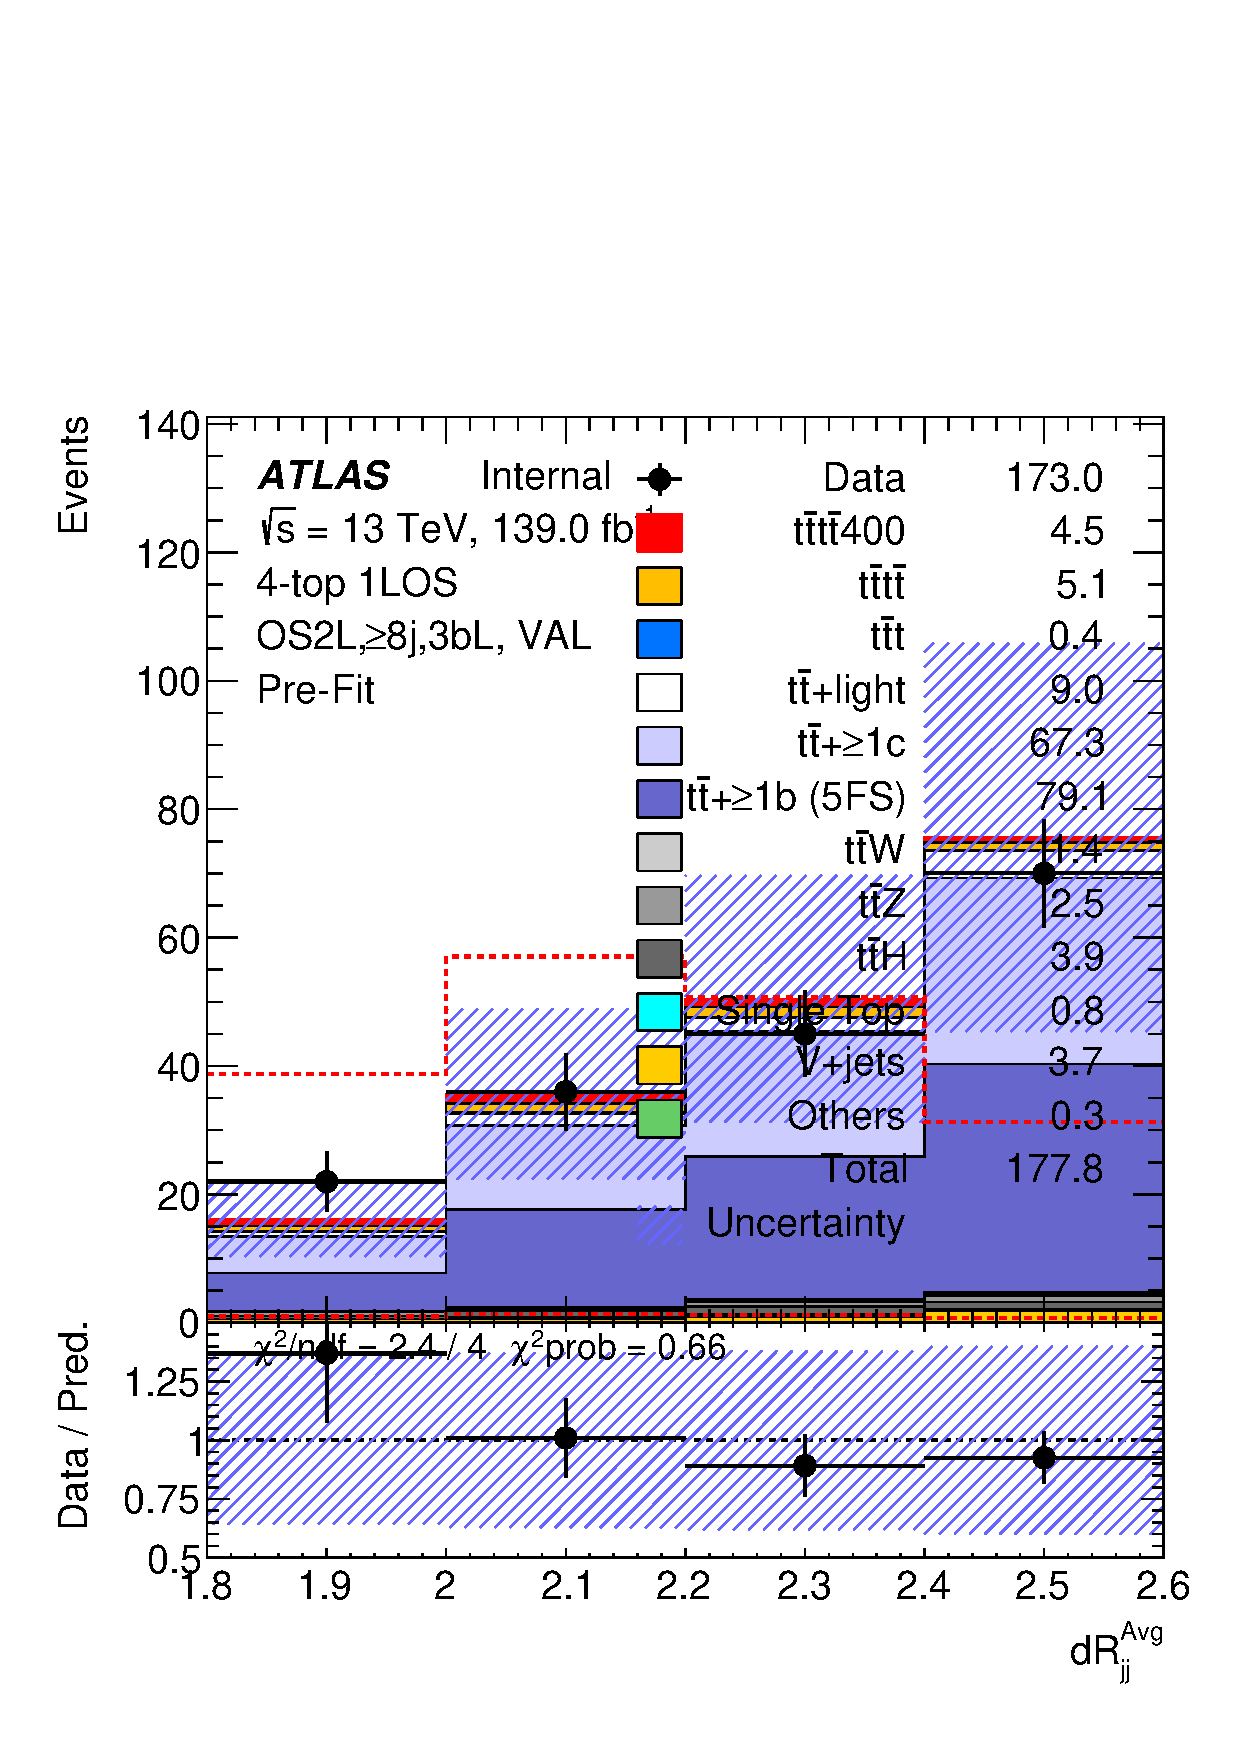
\includegraphics[width=0.23 \textwidth]{figures/fits/GNN/400/all/data_unblindedBonly/Plots/val_os2l_ge8j3bL_dRjj_Avg.pdf} &
        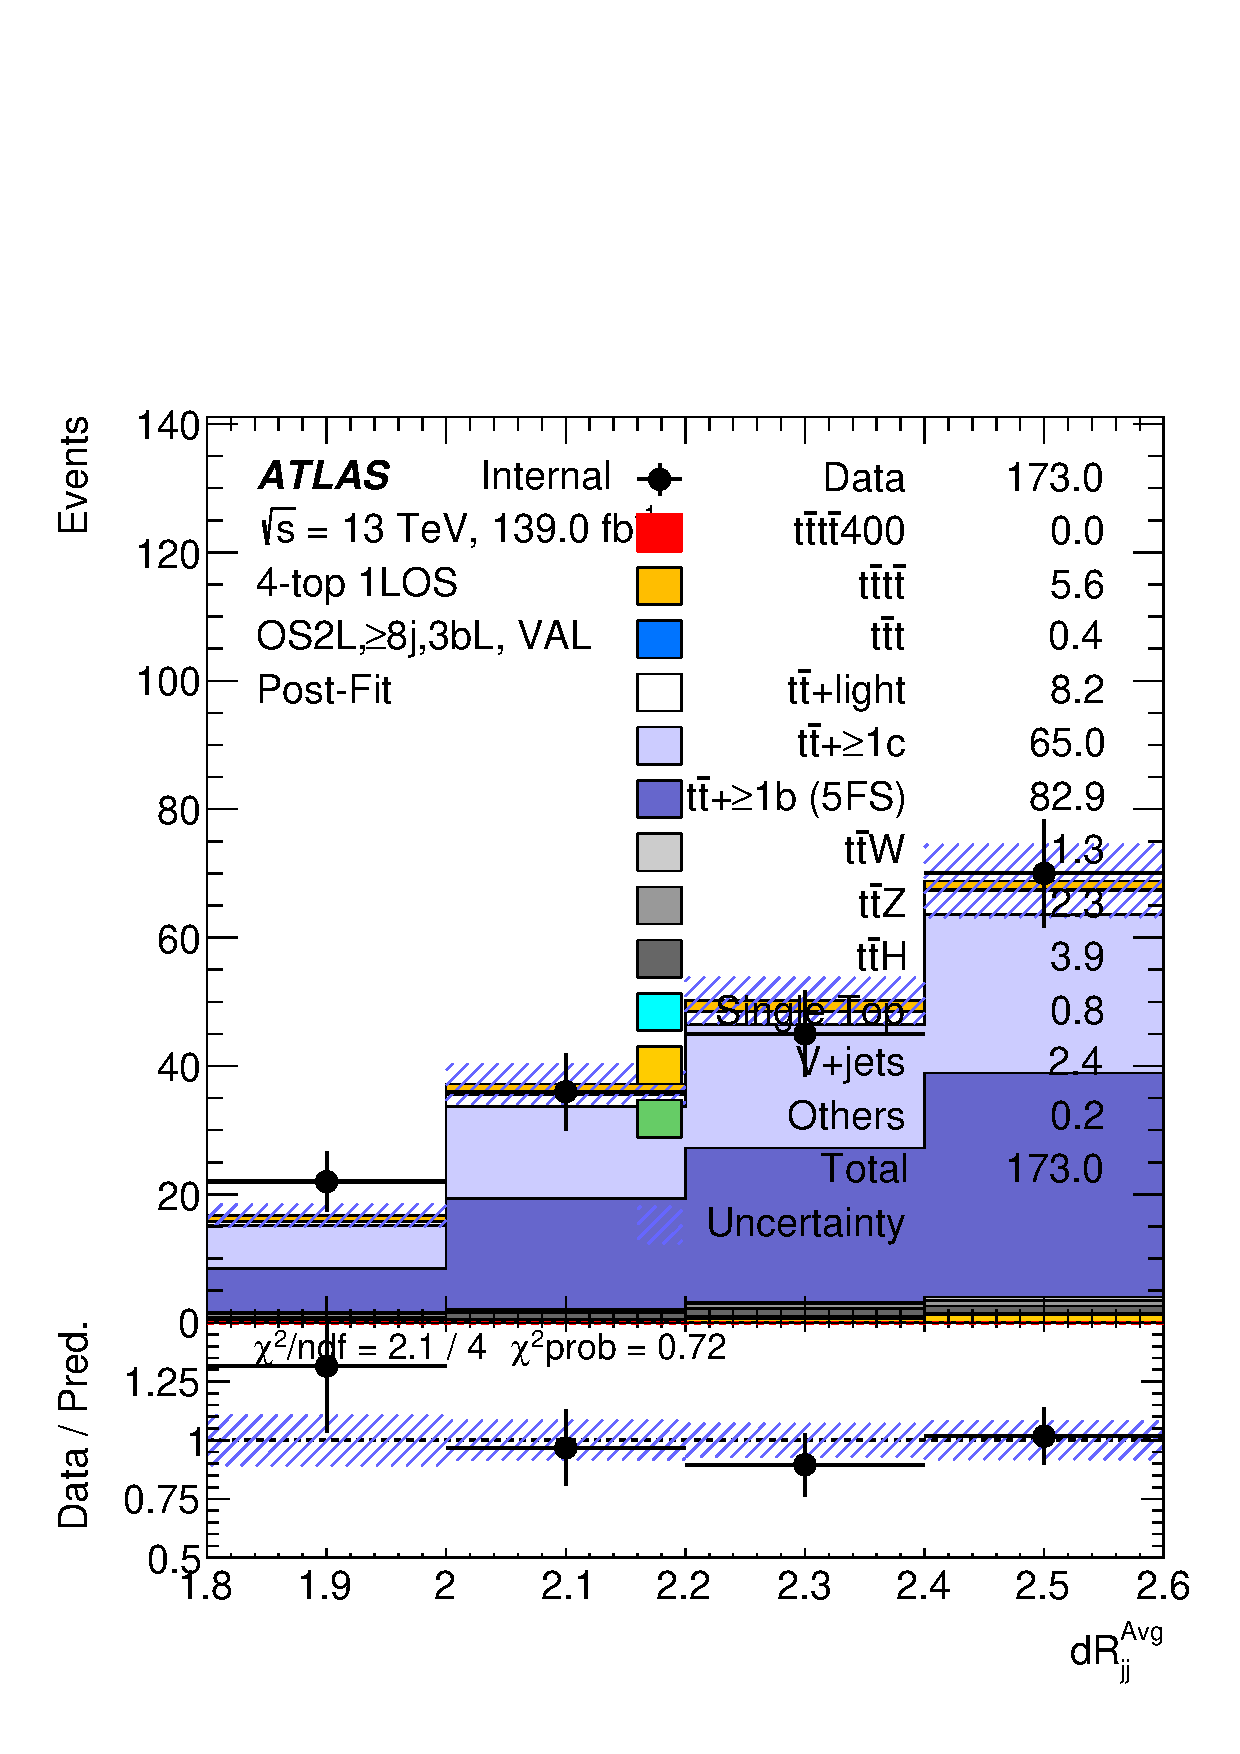
\includegraphics[width=0.23 \textwidth]{figures/fits/GNN/400/all/data_unblindedBonly/Plots/val_os2l_ge8j3bL_dRjj_Avg_postFit.pdf} \\

        \end{tabular}
        \end{center}

\caption{\label{GNN_input_val_1}Pre-fit(left) and Post-fit(right) distributions for GNN input variables in the 2L ge8j3bL region.}
\end{figure}

\begin{figure}

        \begin{center} \setlength{\tabcolsep}{2.5pt}\footnotesize
        \begin{tabular}{cccc}

        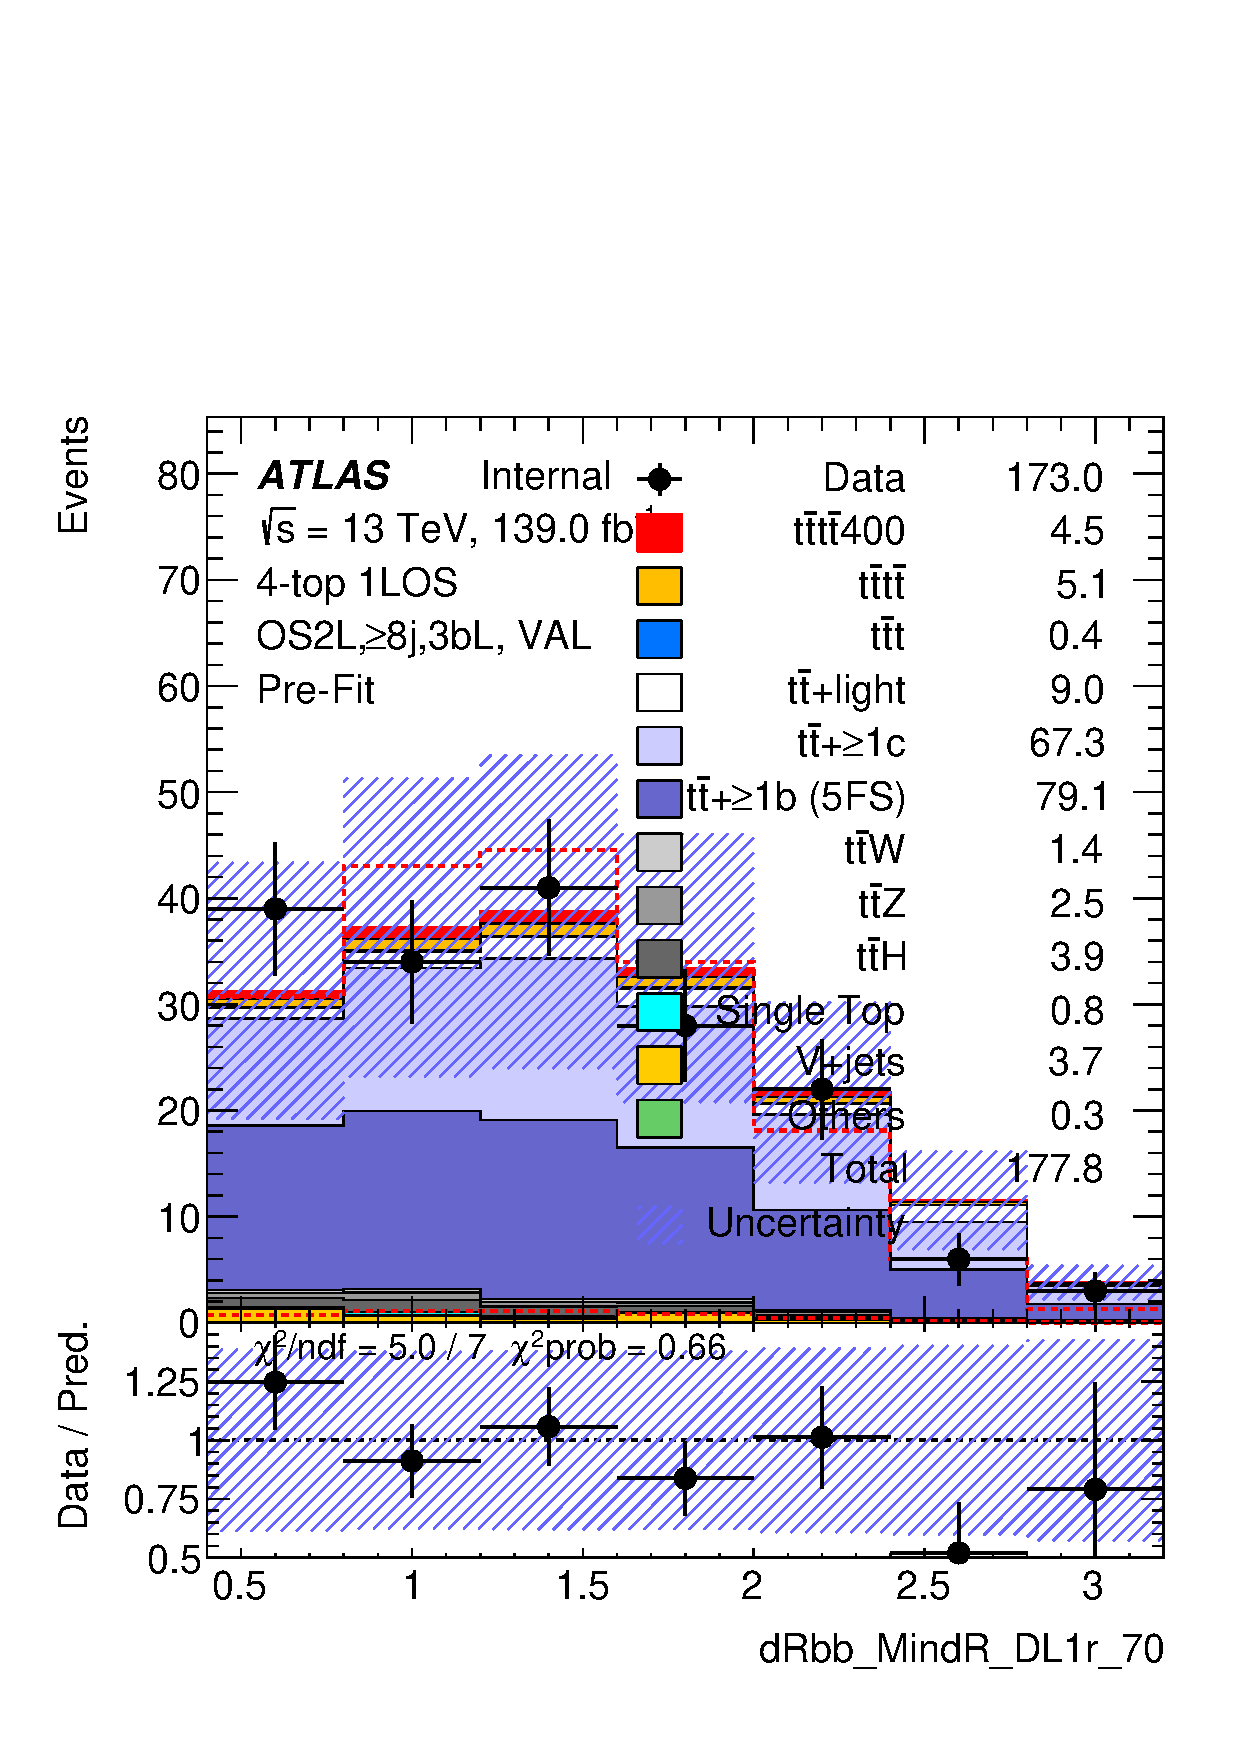
\includegraphics[width=0.23 \textwidth]{figures/fits/GNN/400/all/data_unblindedBonly/Plots/val_os2l_ge8j3bL_dRbb_MindR_DL1r_70.pdf} &
        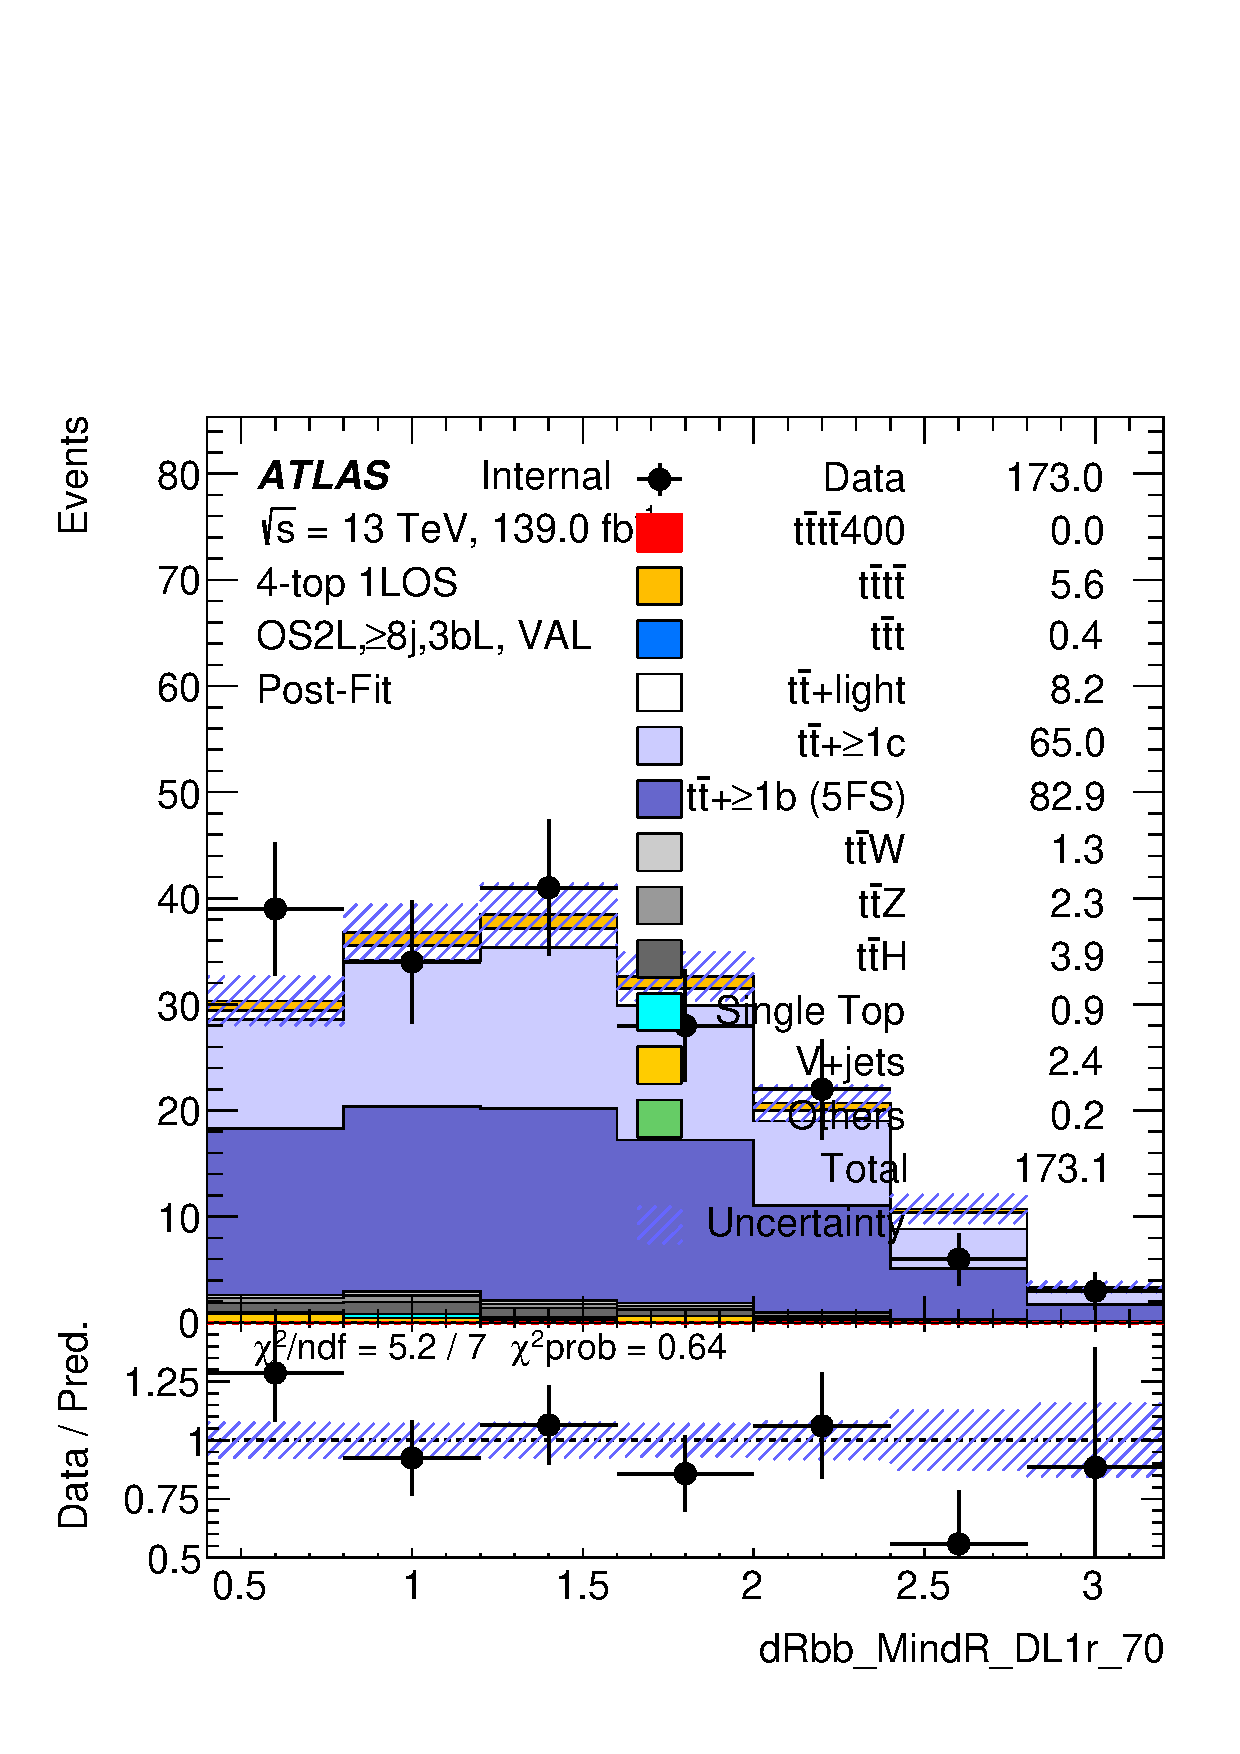
\includegraphics[width=0.23 \textwidth]{figures/fits/GNN/400/all/data_unblindedBonly/Plots/val_os2l_ge8j3bL_dRbb_MindR_DL1r_70_postFit.pdf} &
        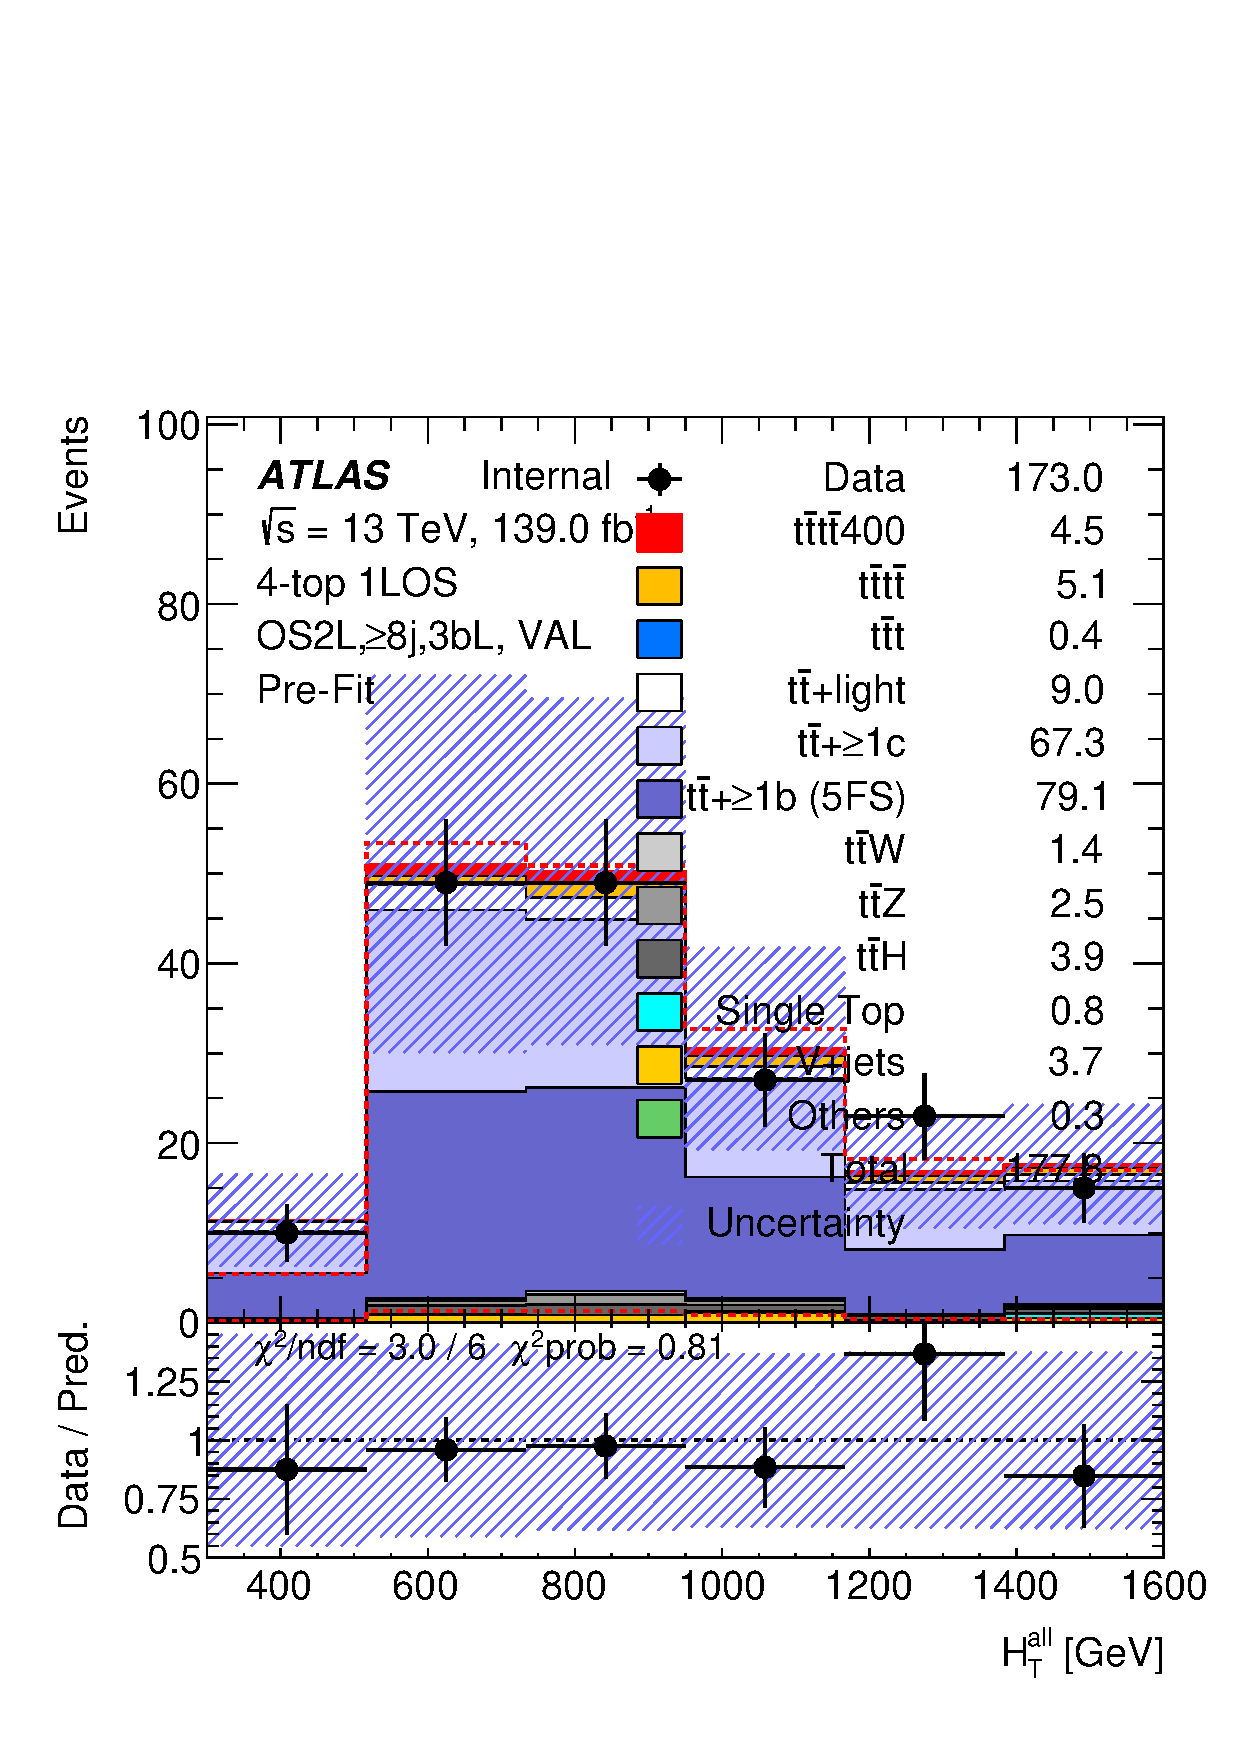
\includegraphics[width=0.23 \textwidth]{figures/fits/GNN/400/all/data_unblindedBonly/Plots/val_os2l_ge8j3bL_HT_all.pdf} &
        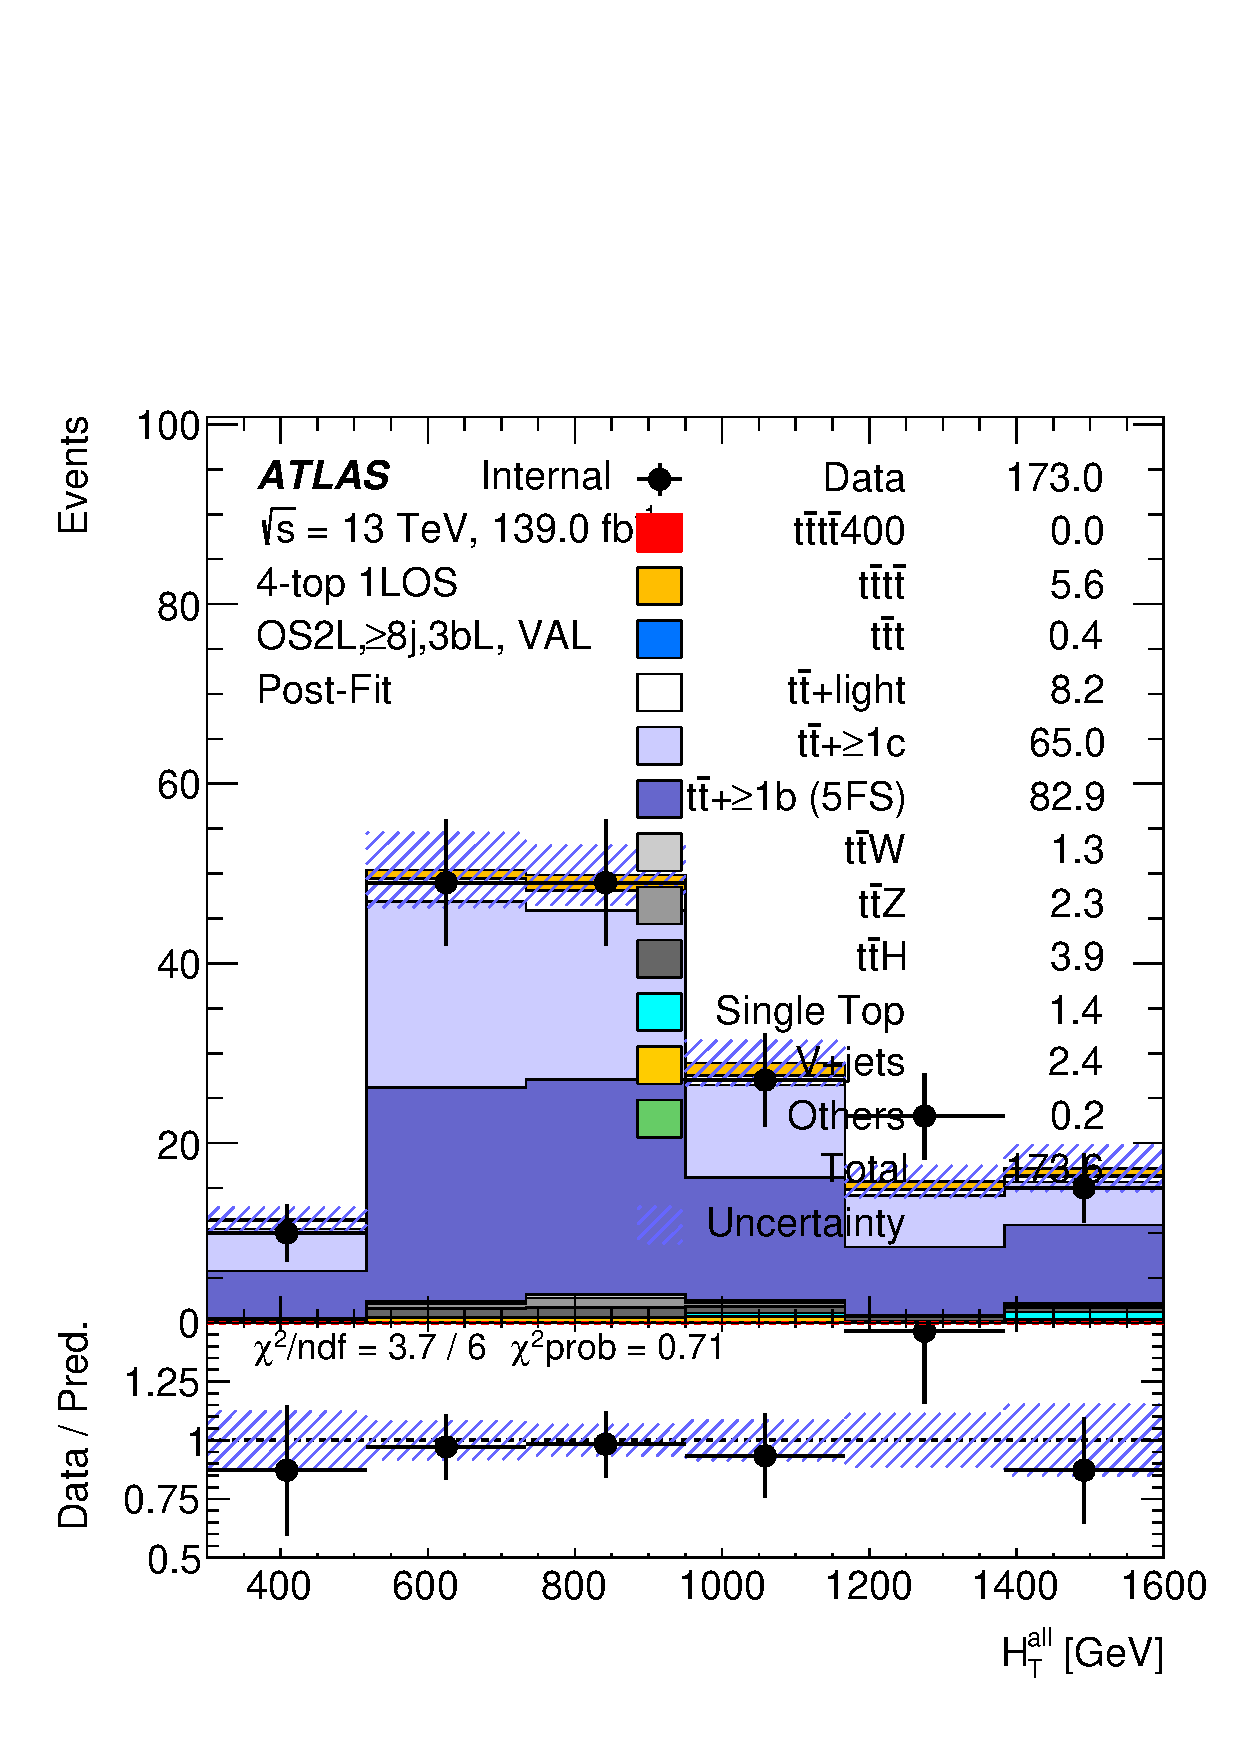
\includegraphics[width=0.23 \textwidth]{figures/fits/GNN/400/all/data_unblindedBonly/Plots/val_os2l_ge8j3bL_HT_all_postFit.pdf} \\

        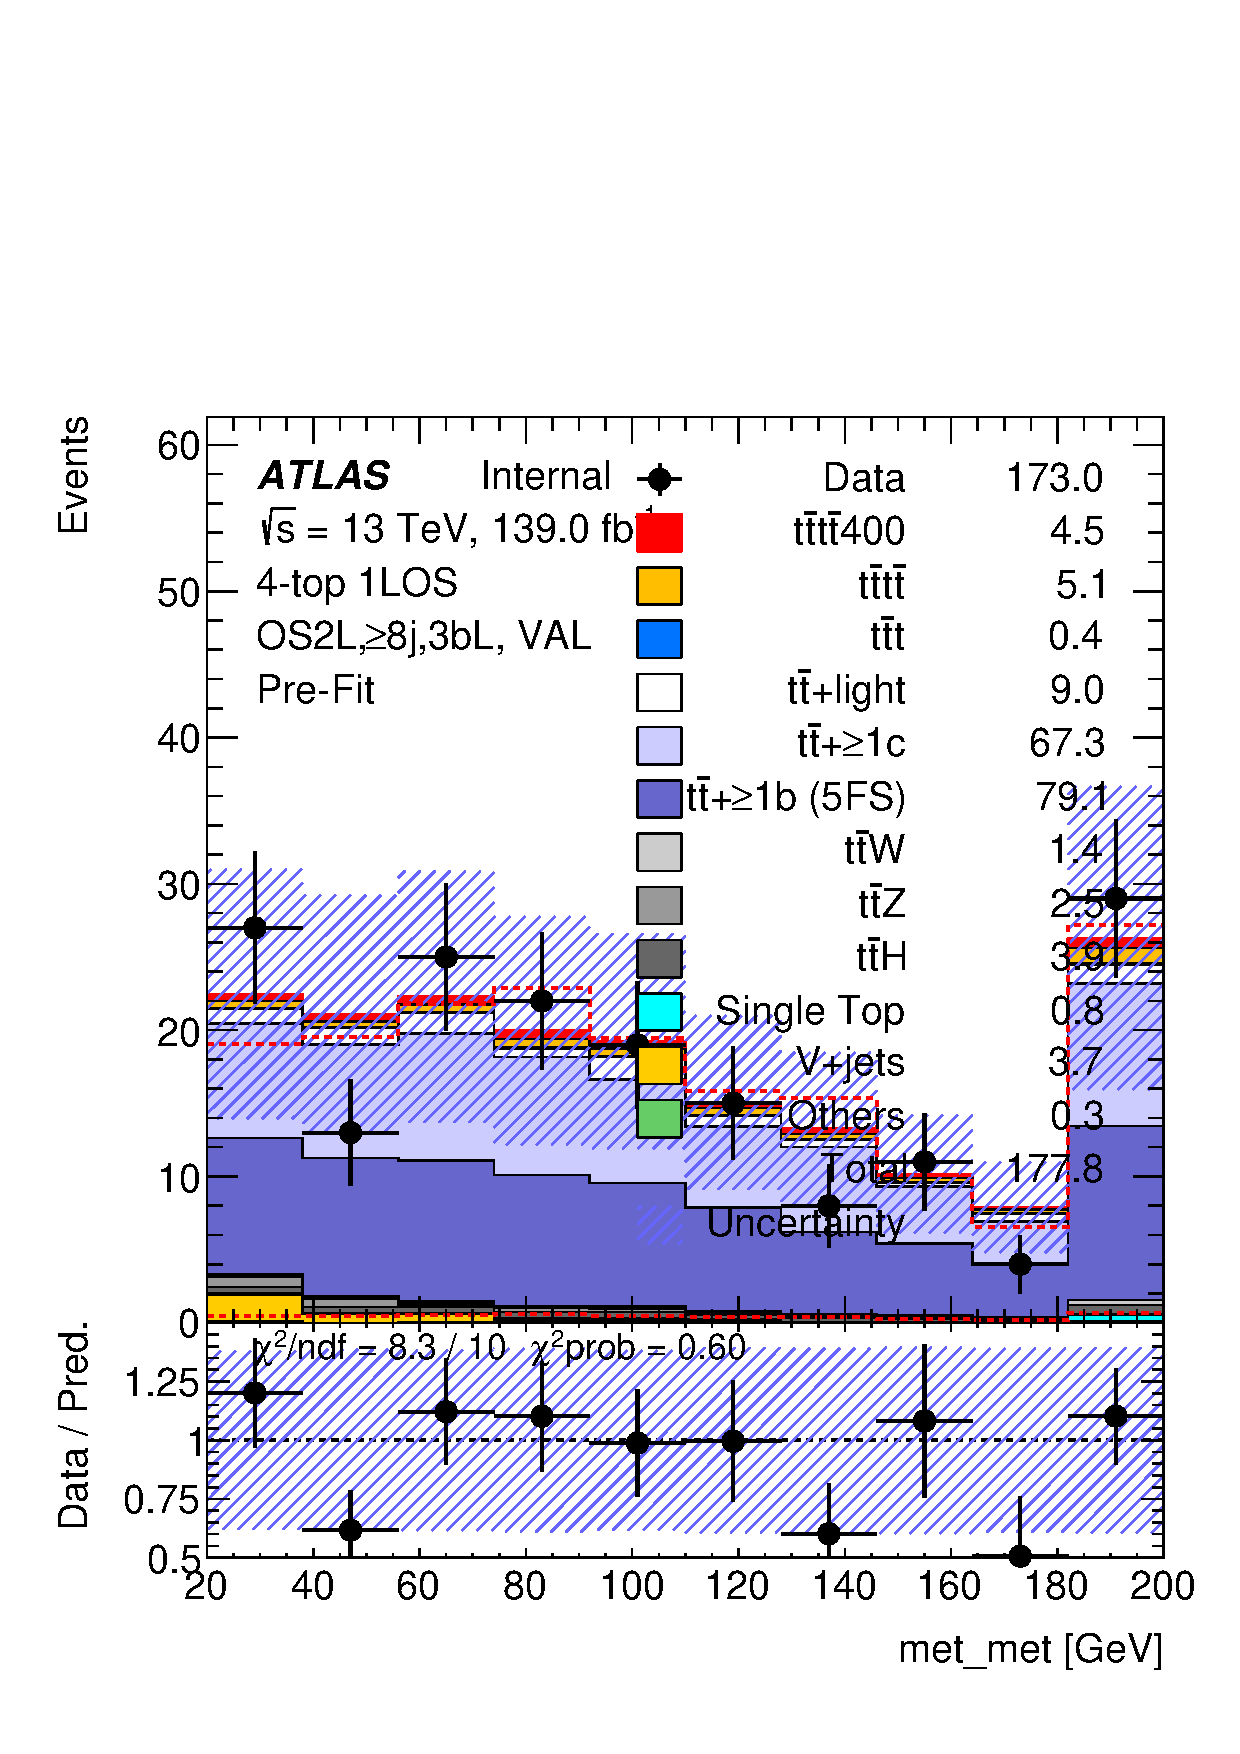
\includegraphics[width=0.23 \textwidth]{figures/fits/GNN/400/all/data_unblindedBonly/Plots/val_os2l_ge8j3bL_met.pdf} &
        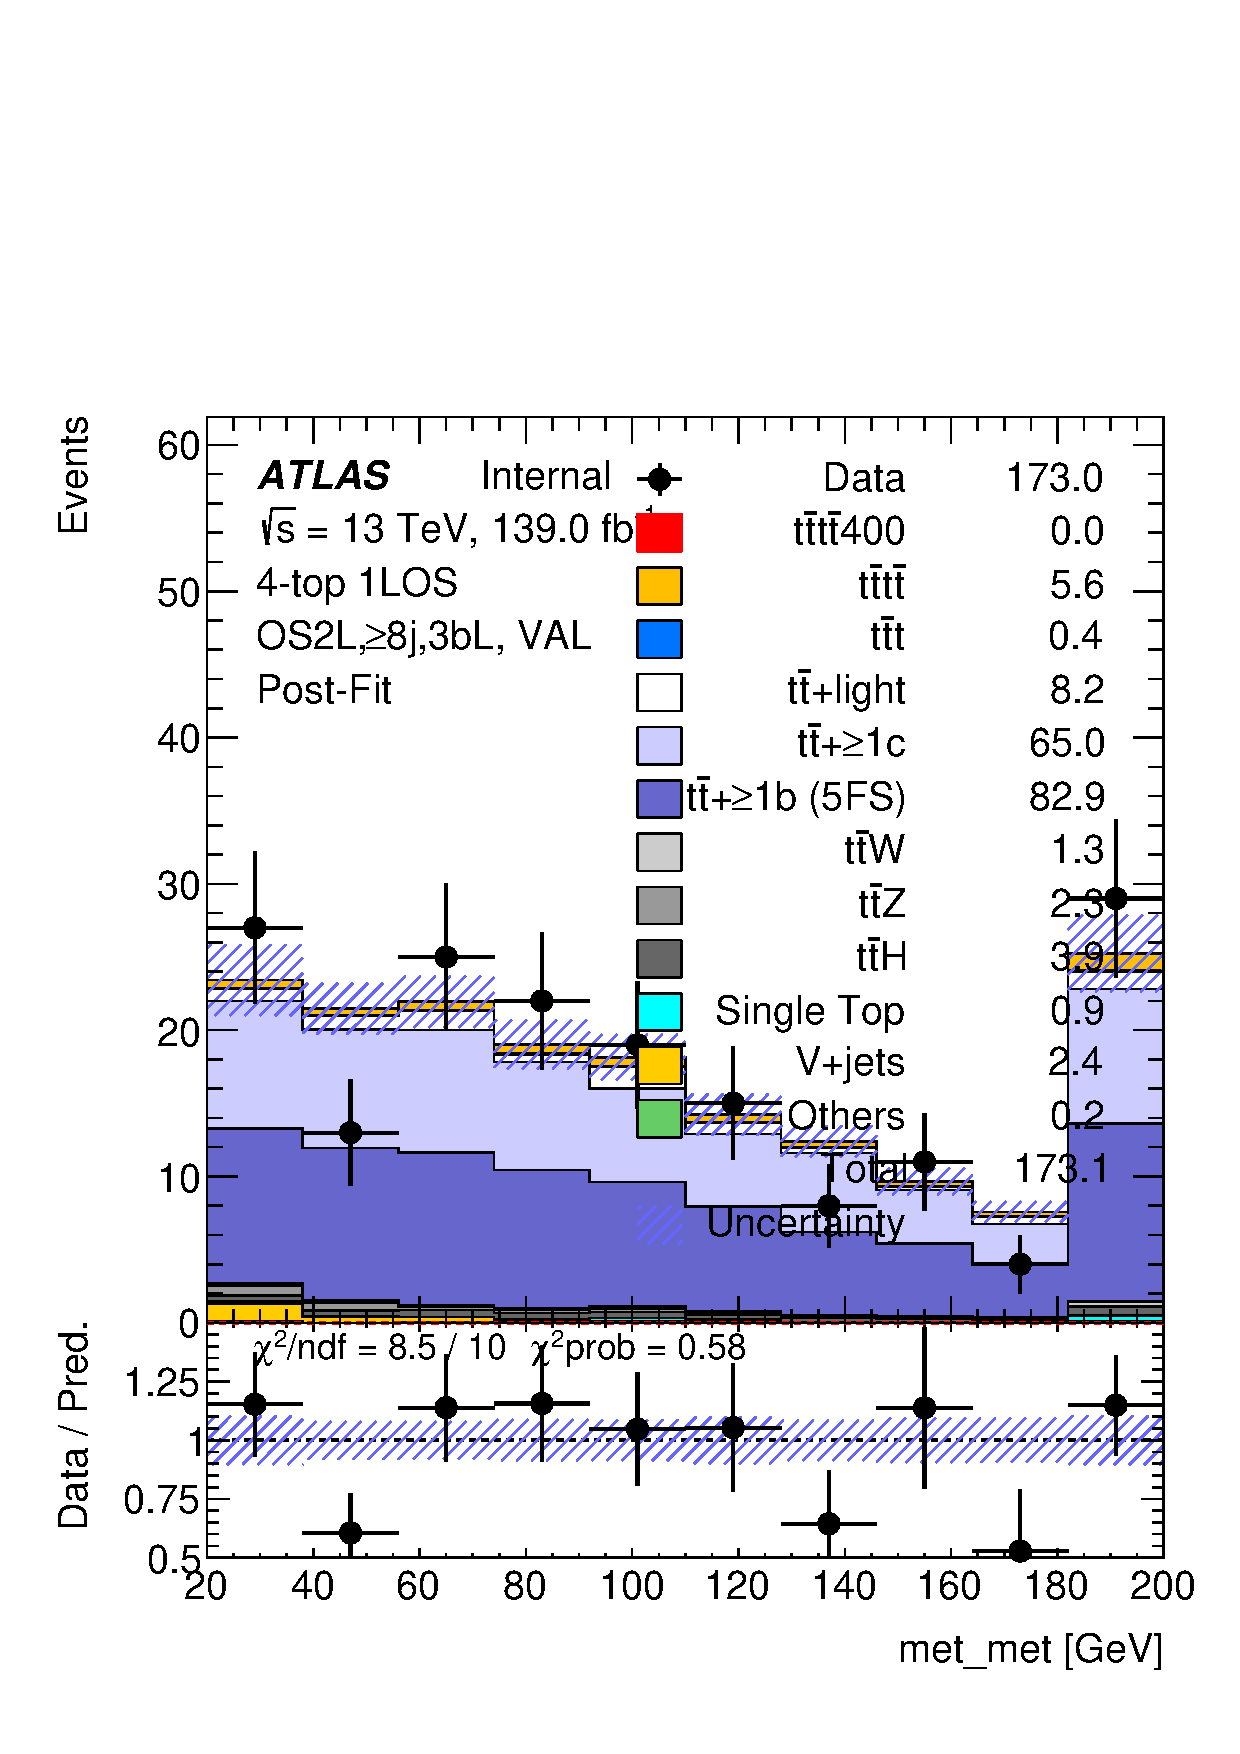
\includegraphics[width=0.23 \textwidth]{figures/fits/GNN/400/all/data_unblindedBonly/Plots/val_os2l_ge8j3bL_met_postFit.pdf} &
        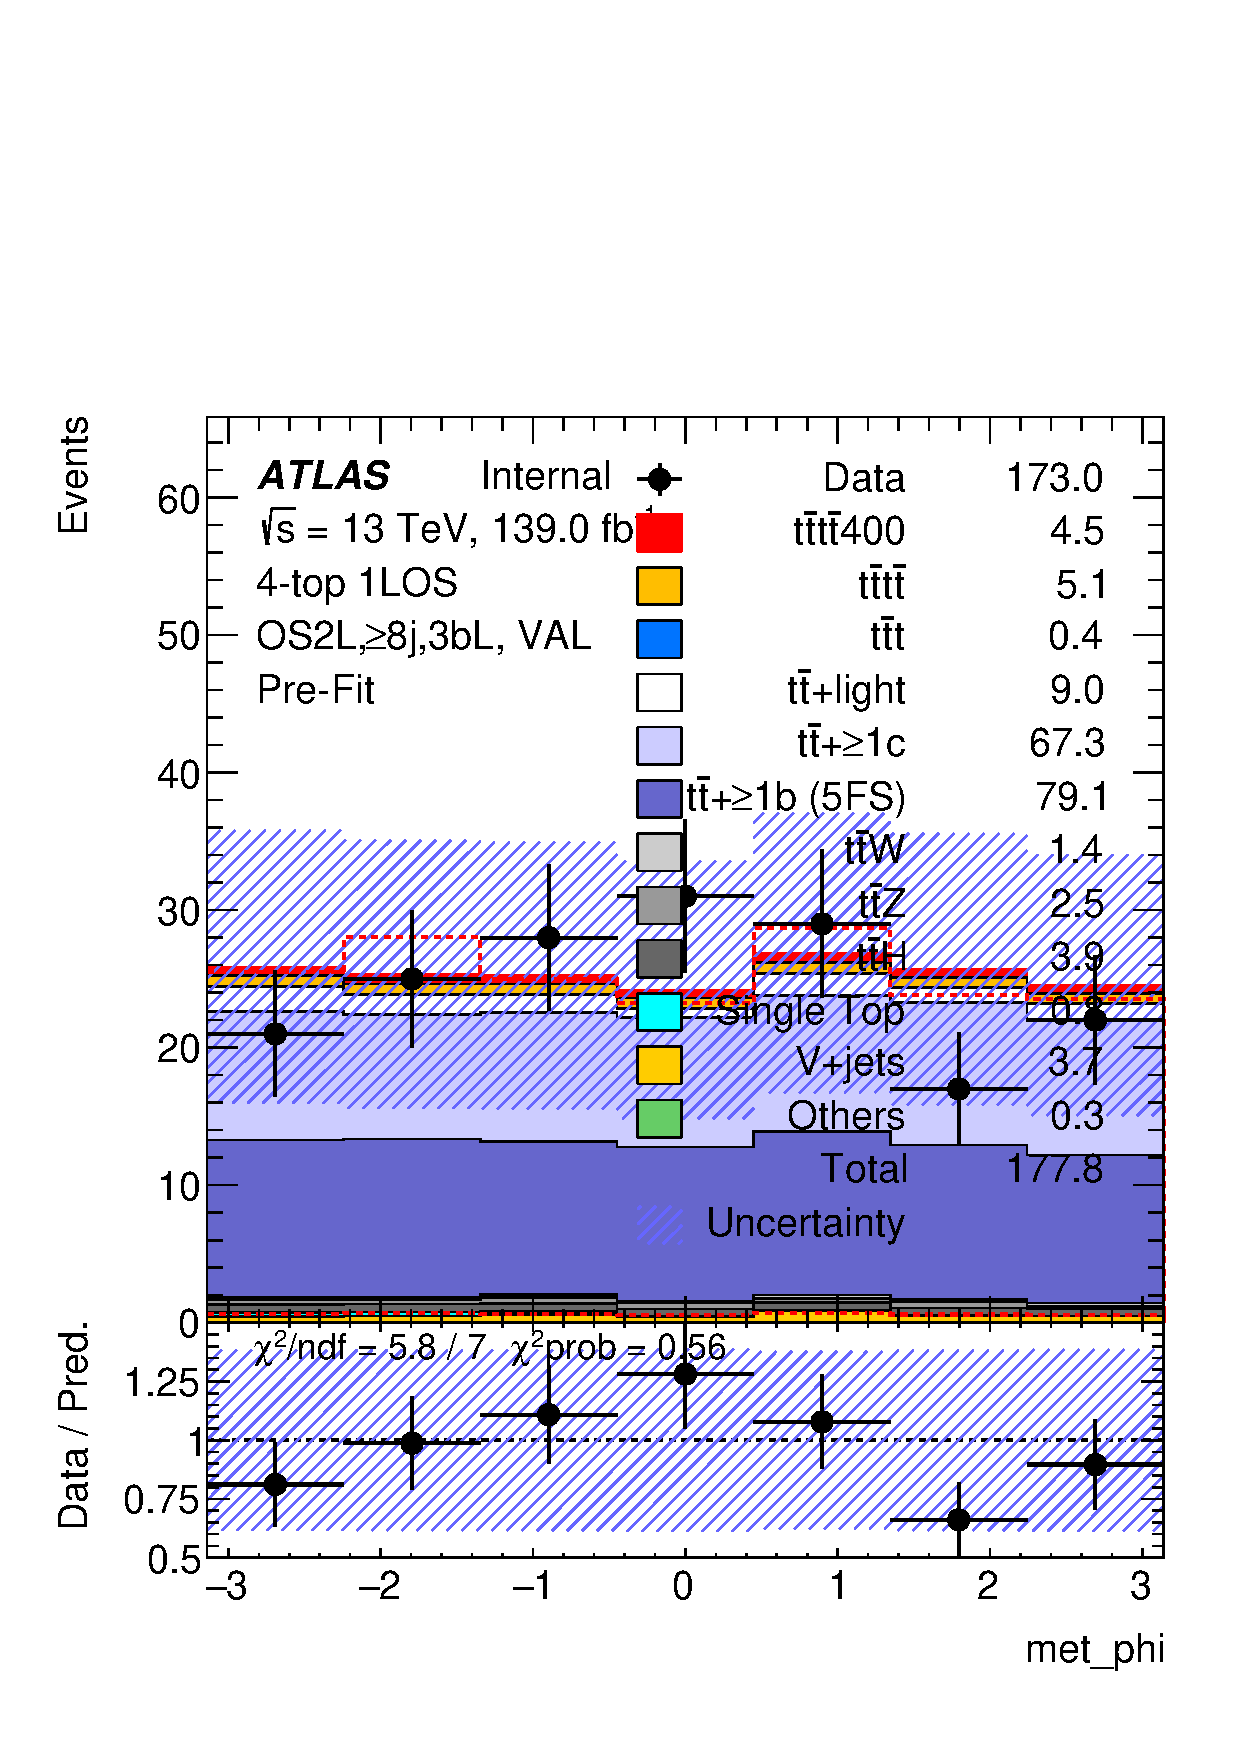
\includegraphics[width=0.23 \textwidth]{figures/fits/GNN/400/all/data_unblindedBonly/Plots/val_os2l_ge8j3bL_met_phi.pdf} &
        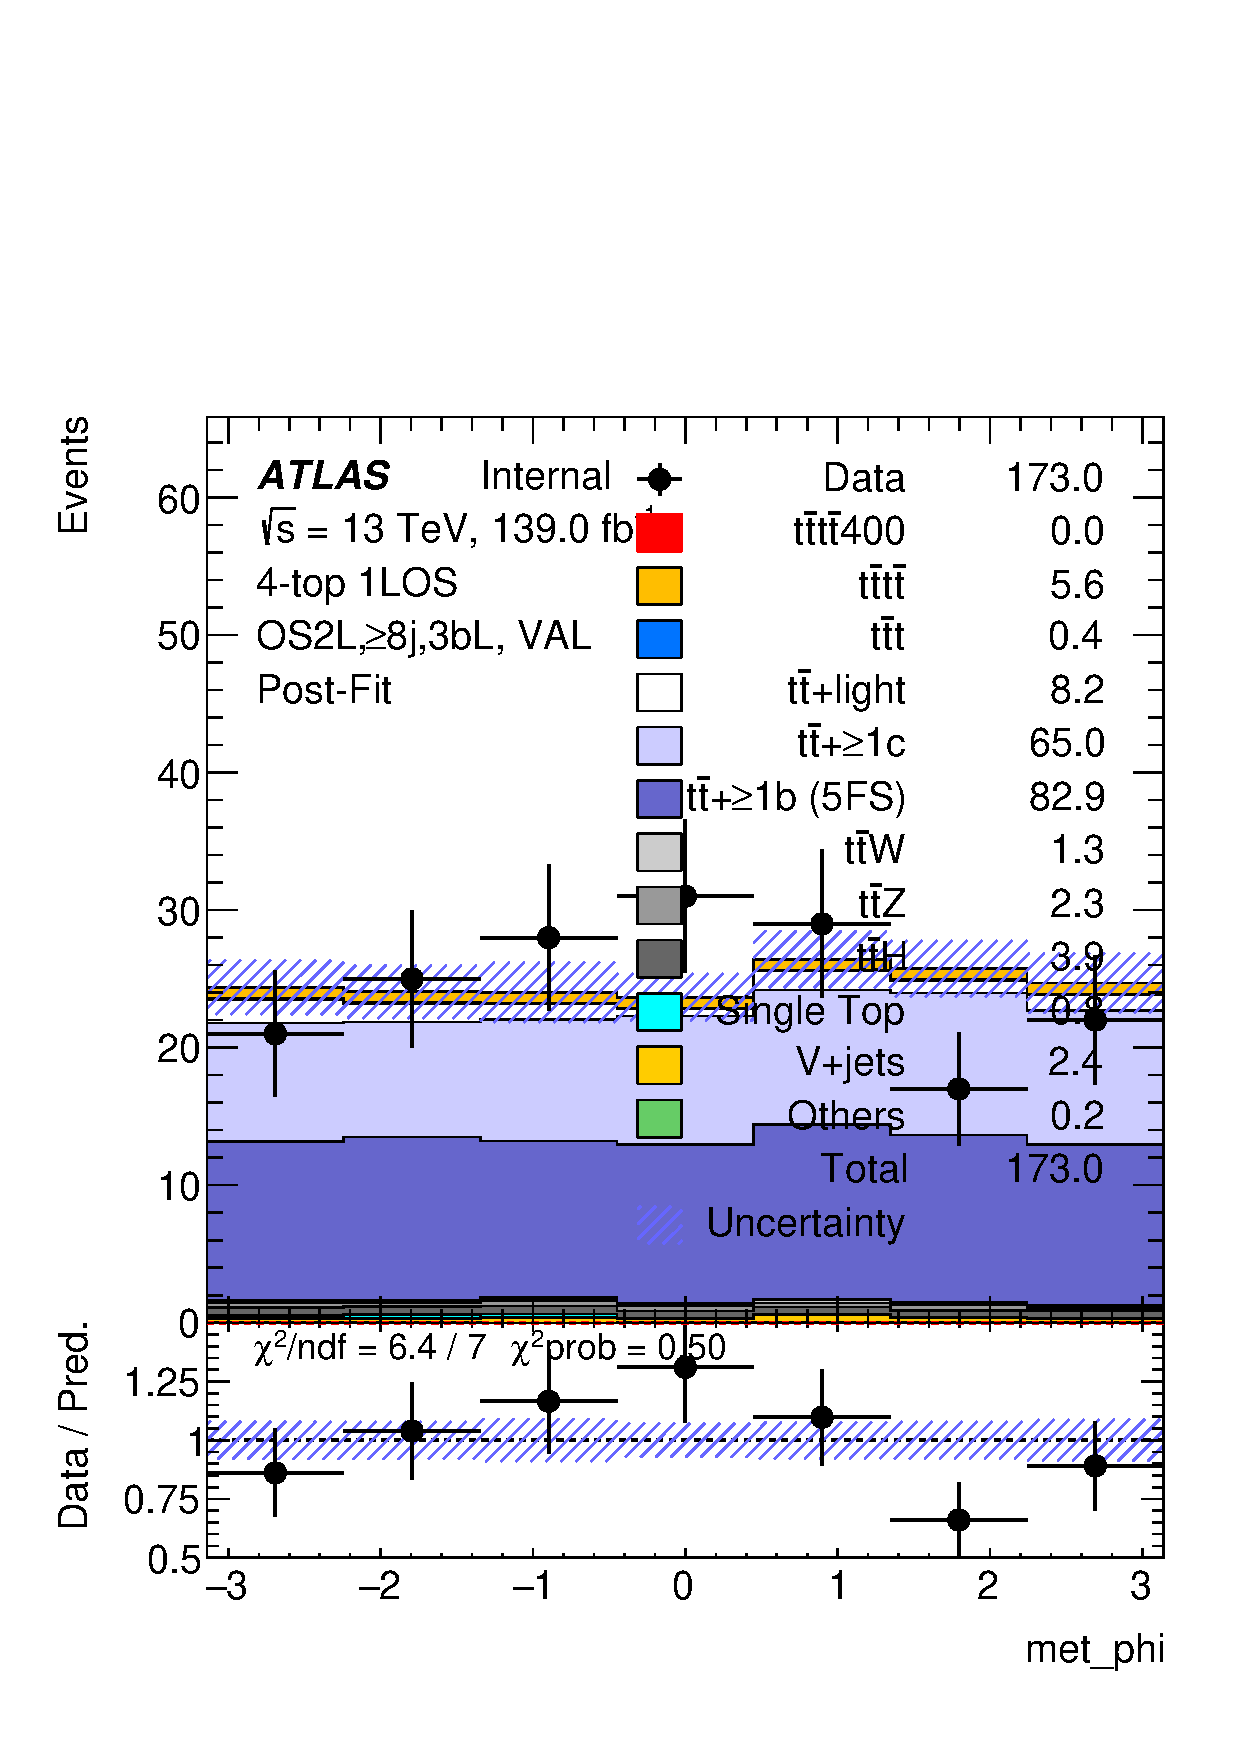
\includegraphics[width=0.23 \textwidth]{figures/fits/GNN/400/all/data_unblindedBonly/Plots/val_os2l_ge8j3bL_met_phi_postFit.pdf} \\

        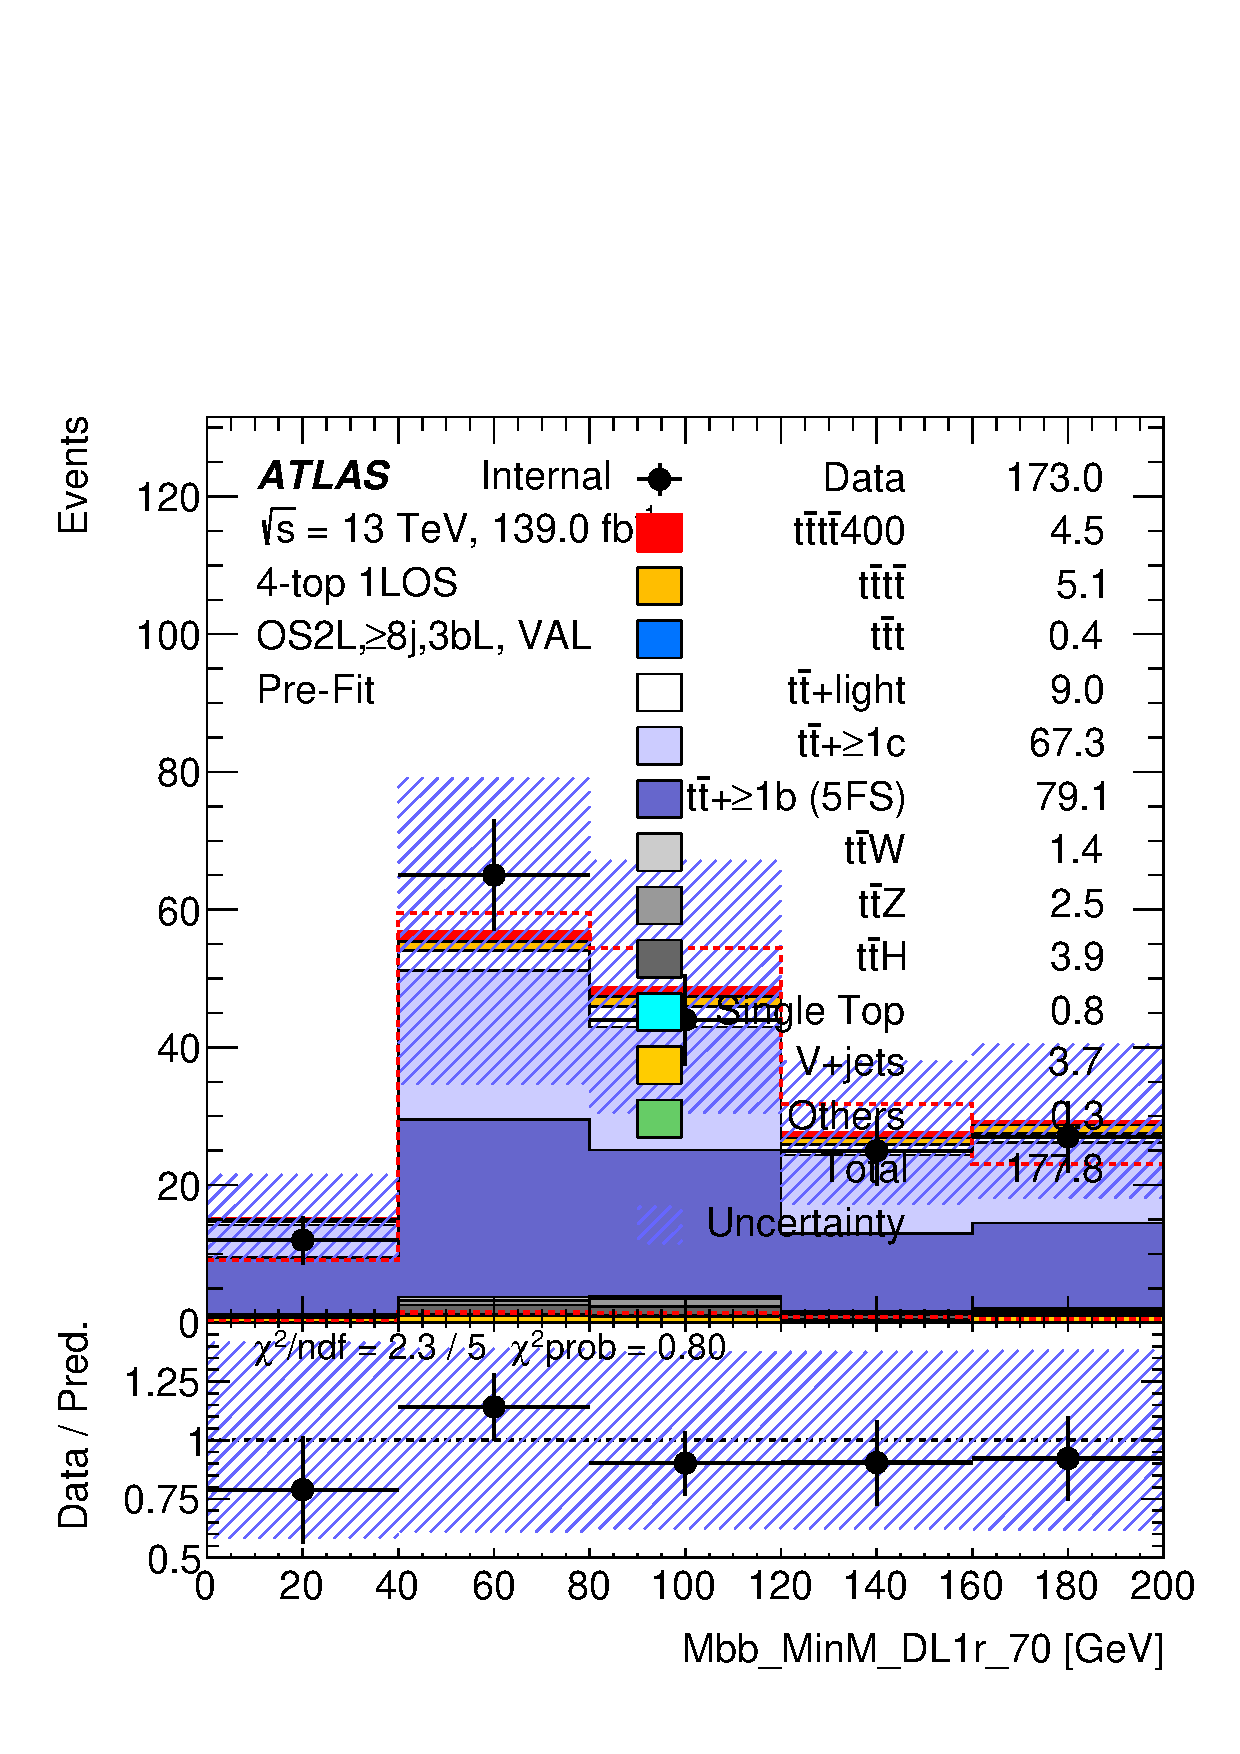
\includegraphics[width=0.23 \textwidth]{figures/fits/GNN/400/all/data_unblindedBonly/Plots/val_os2l_ge8j3bL_Mbb_MinM_DL1r_70.pdf} &
        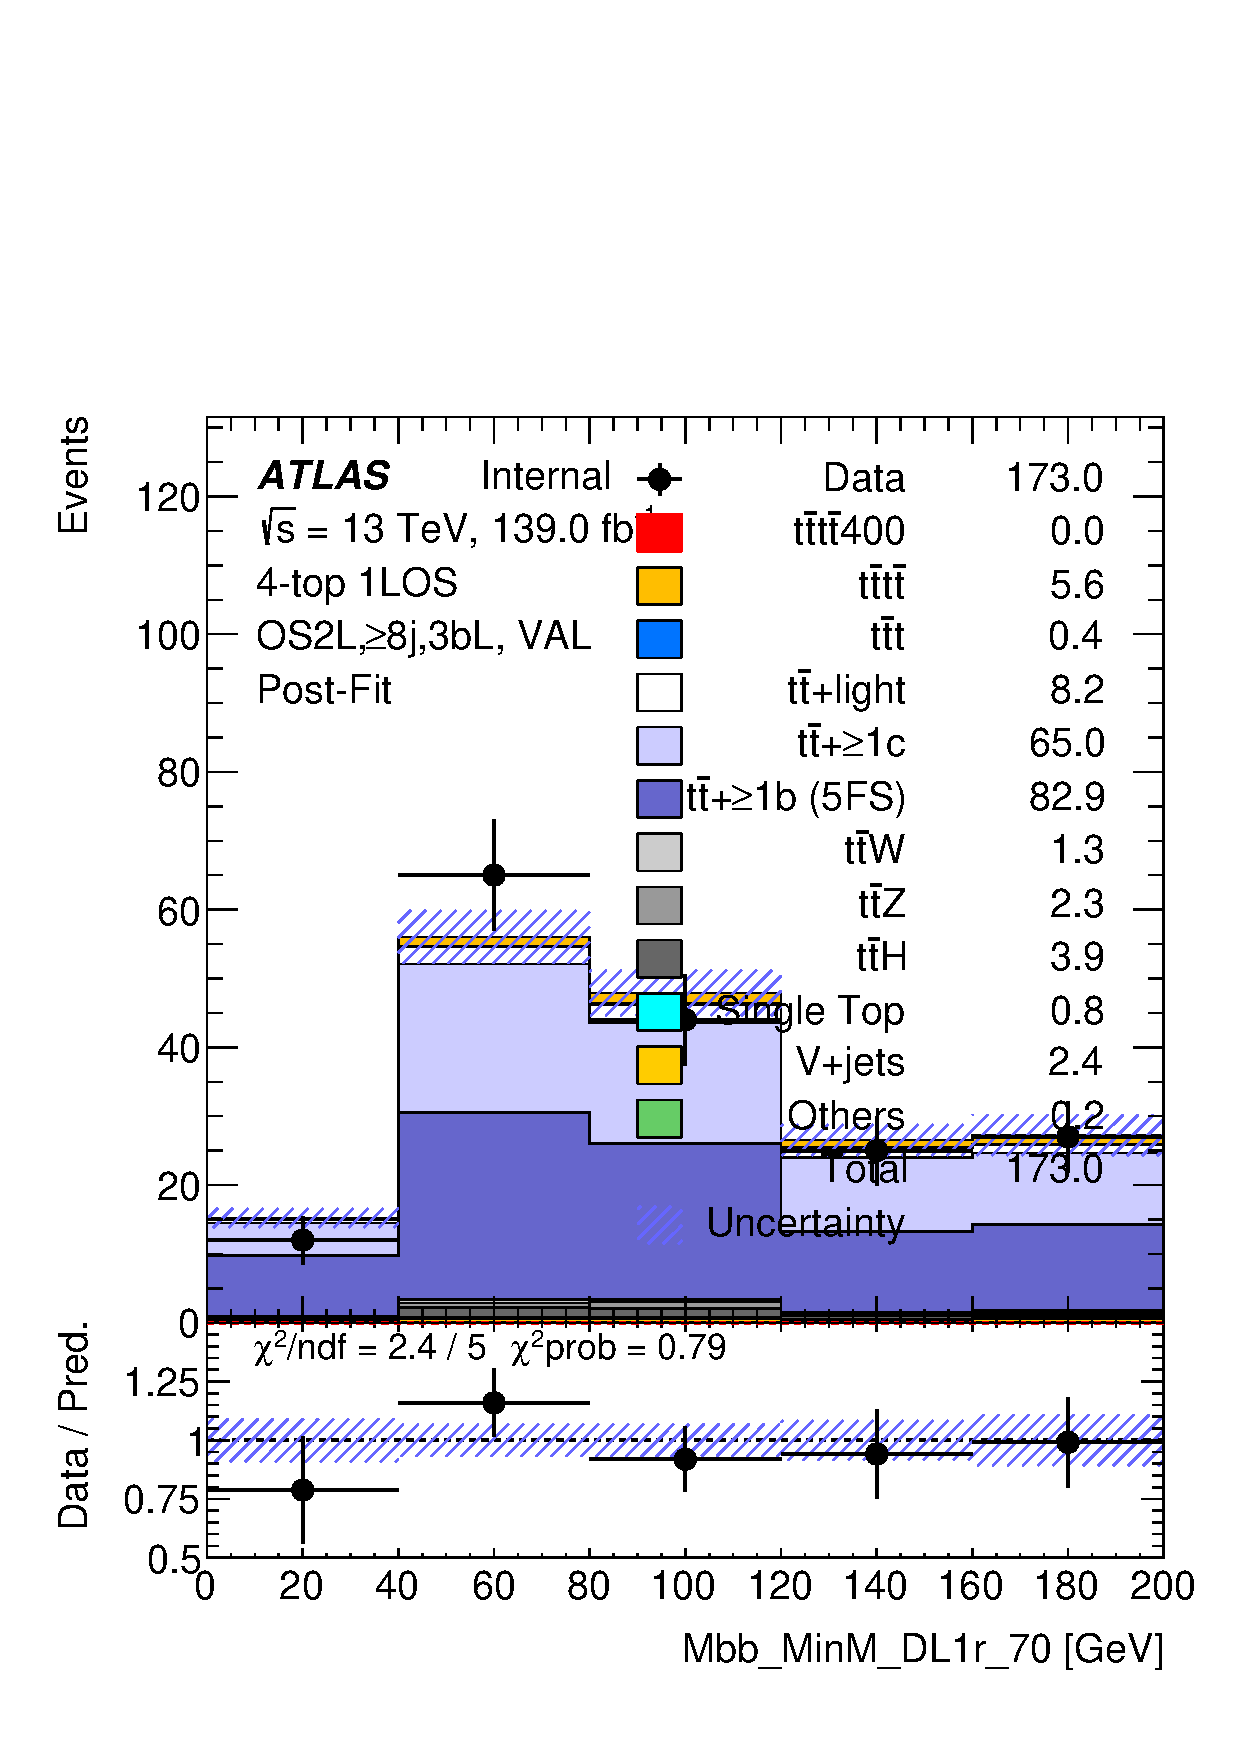
\includegraphics[width=0.23 \textwidth]{figures/fits/GNN/400/all/data_unblindedBonly/Plots/val_os2l_ge8j3bL_Mbb_MinM_DL1r_70_postFit.pdf} &
        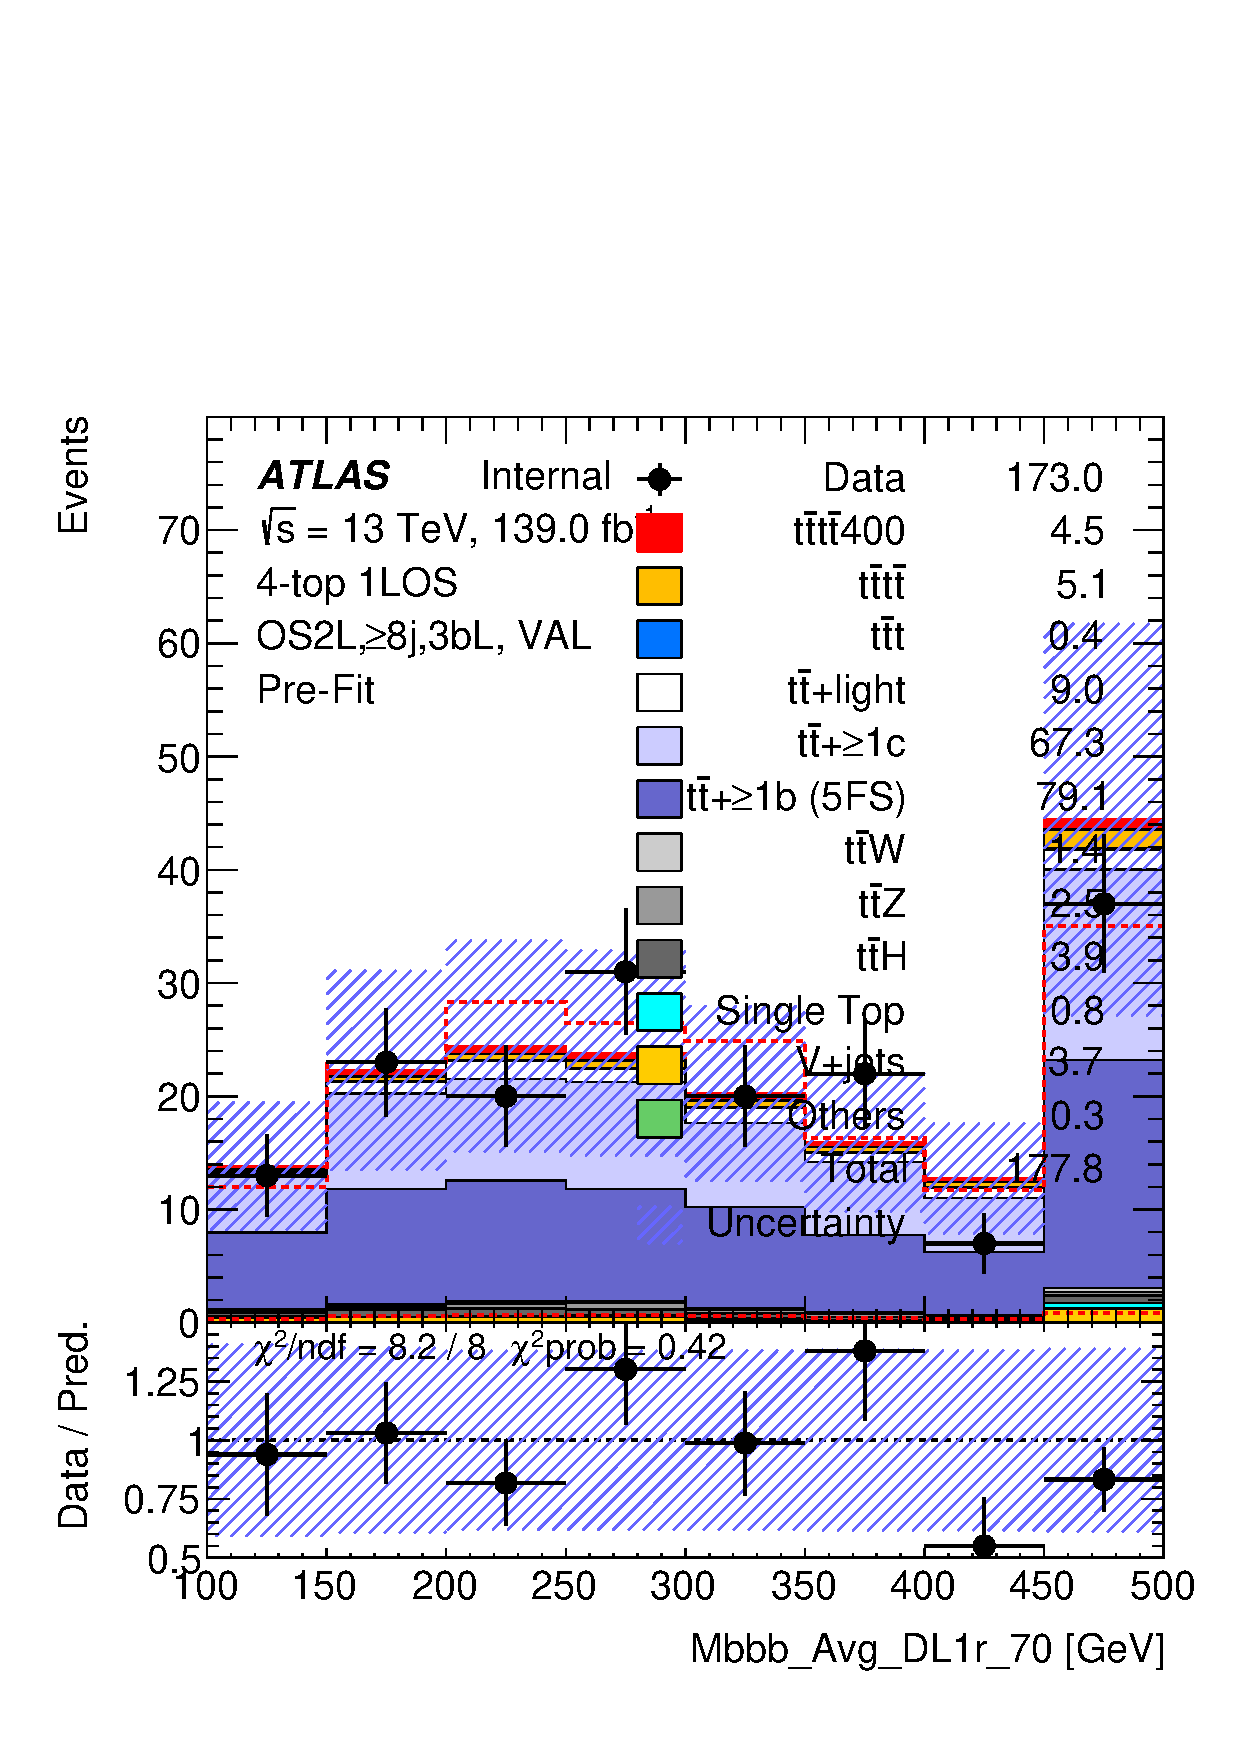
\includegraphics[width=0.23 \textwidth]{figures/fits/GNN/400/all/data_unblindedBonly/Plots/val_os2l_ge8j3bL_Mbbb_Avg_DL1r_70.pdf} &
        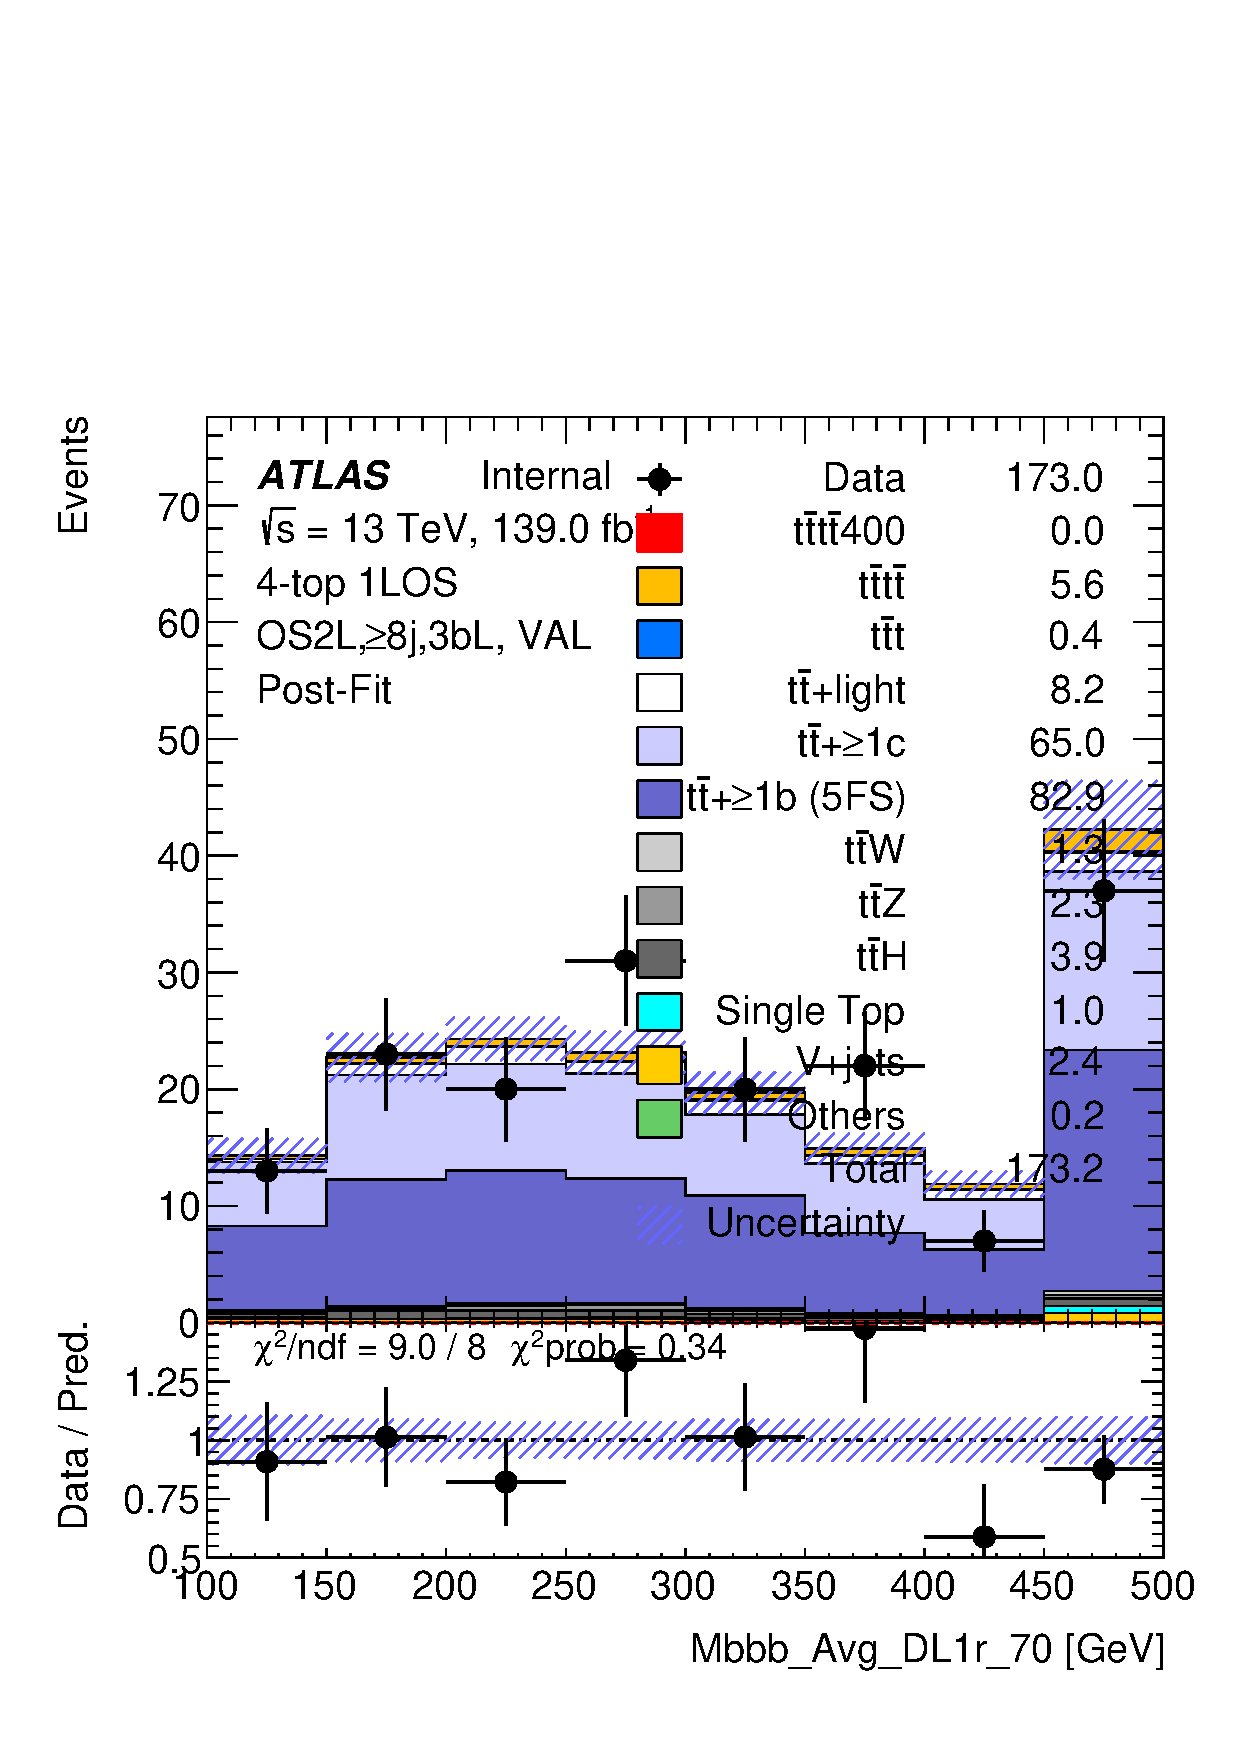
\includegraphics[width=0.23 \textwidth]{figures/fits/GNN/400/all/data_unblindedBonly/Plots/val_os2l_ge8j3bL_Mbbb_Avg_DL1r_70_postFit.pdf} \\

        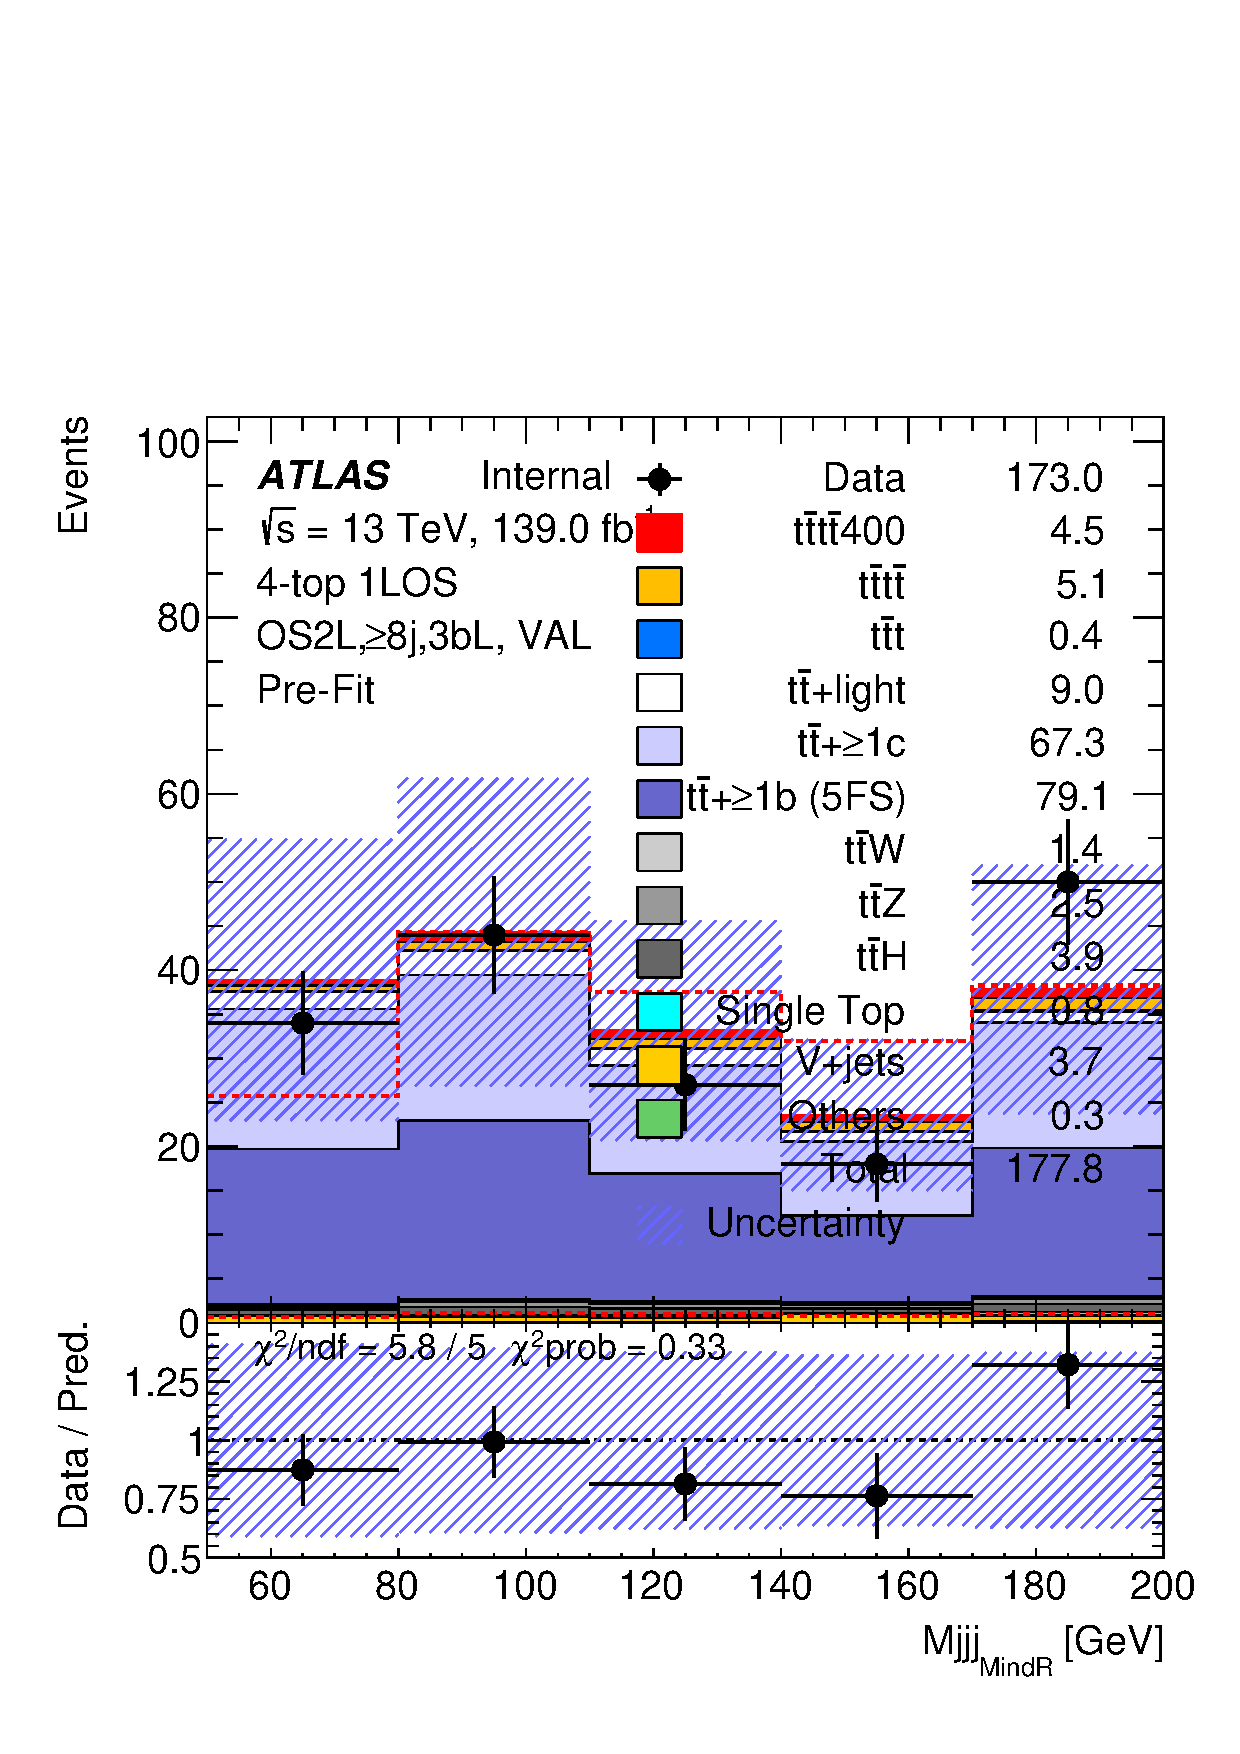
\includegraphics[width=0.23 \textwidth]{figures/fits/GNN/400/all/data_unblindedBonly/Plots/val_os2l_ge8j3bL_Mjjj_MindR.pdf} &
        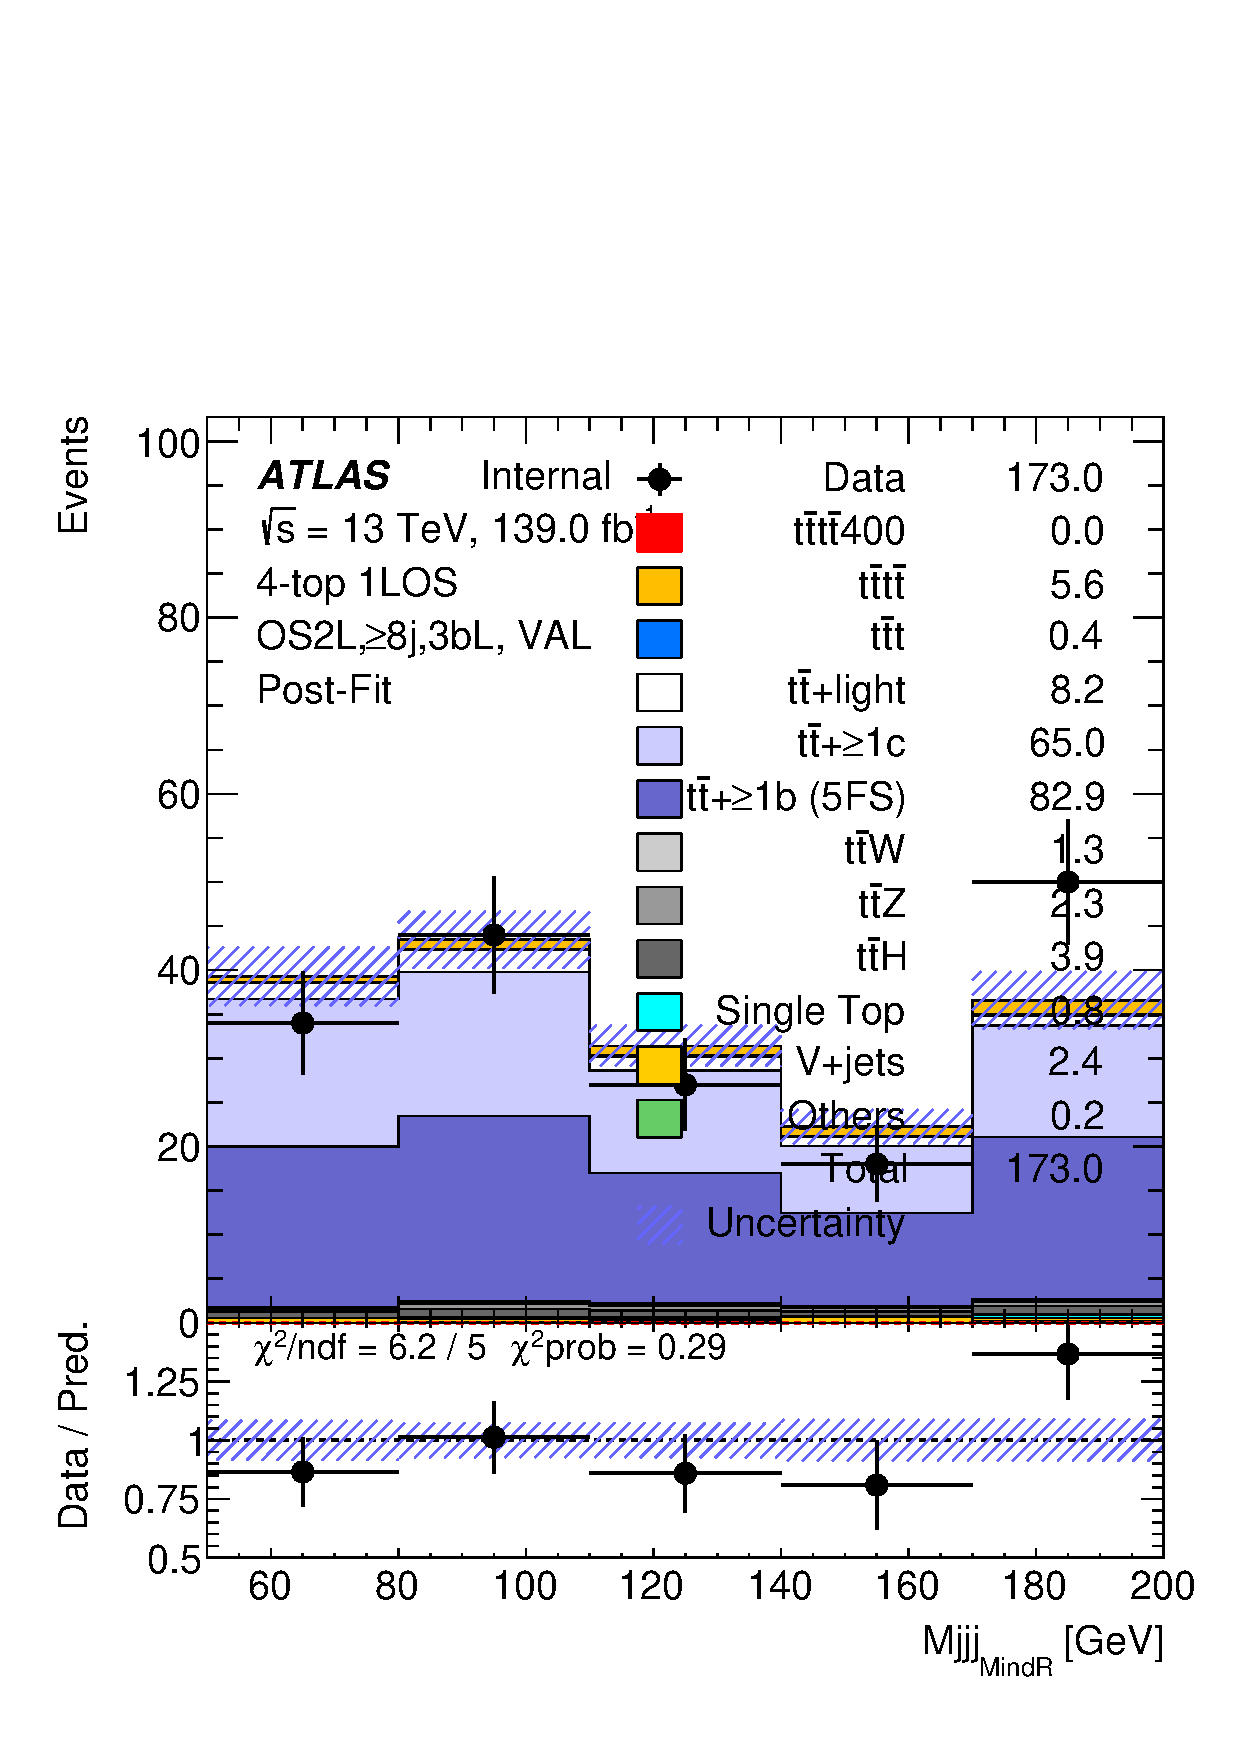
\includegraphics[width=0.23 \textwidth]{figures/fits/GNN/400/all/data_unblindedBonly/Plots/val_os2l_ge8j3bL_Mjjj_MindR_postFit.pdf} &
        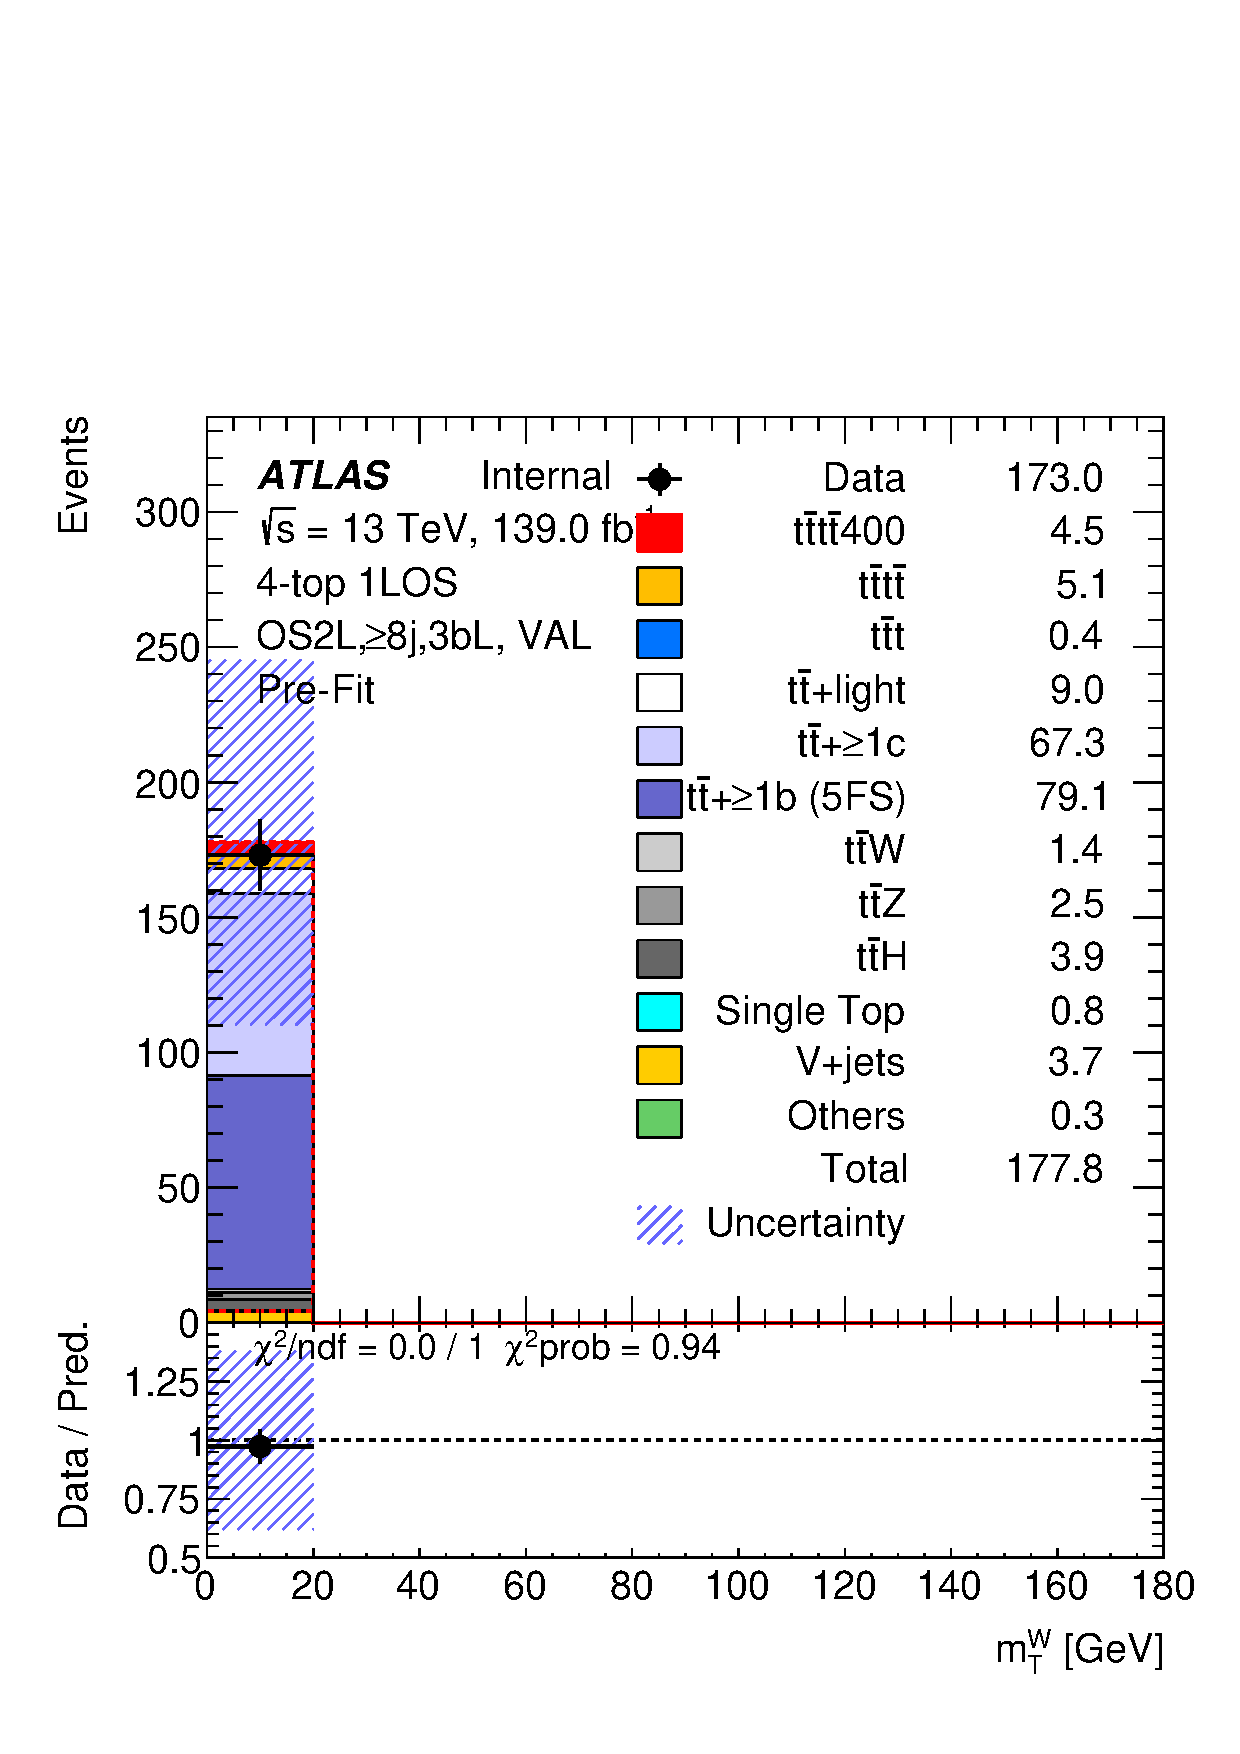
\includegraphics[width=0.23 \textwidth]{figures/fits/GNN/400/all/data_unblindedBonly/Plots/val_os2l_ge8j3bL_mtw.pdf} &
        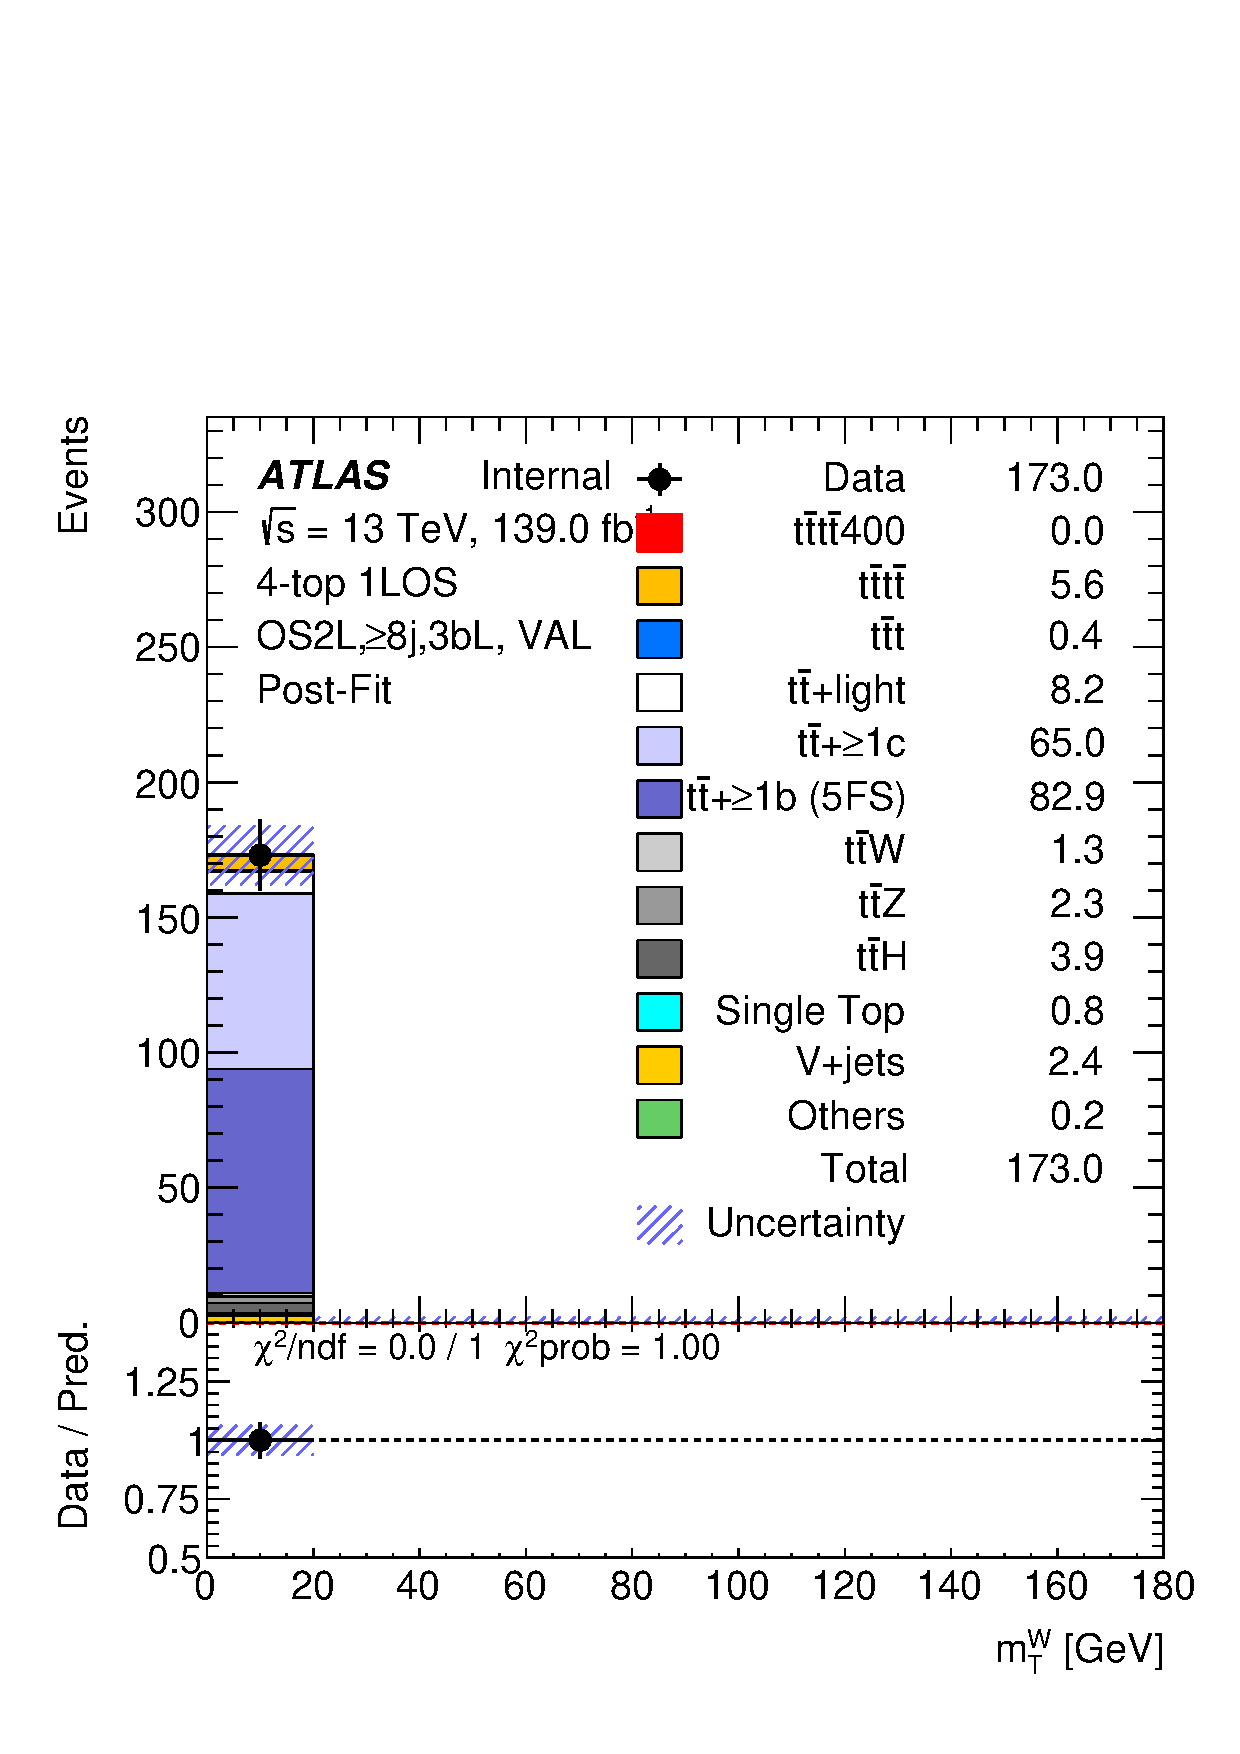
\includegraphics[width=0.23 \textwidth]{figures/fits/GNN/400/all/data_unblindedBonly/Plots/val_os2l_ge8j3bL_mtw_postFit.pdf} \\

        \end{tabular}
        \end{center}

\caption{\label{GNN_input_val_2}Pre-fit(left) and Post-fit(right) distributions for GNN input variables in the 2L ge8j3bL region.}
\end{figure}

\begin{figure}

        \begin{center} \setlength{\tabcolsep}{2.5pt}\footnotesize
        \begin{tabular}{cccc}

        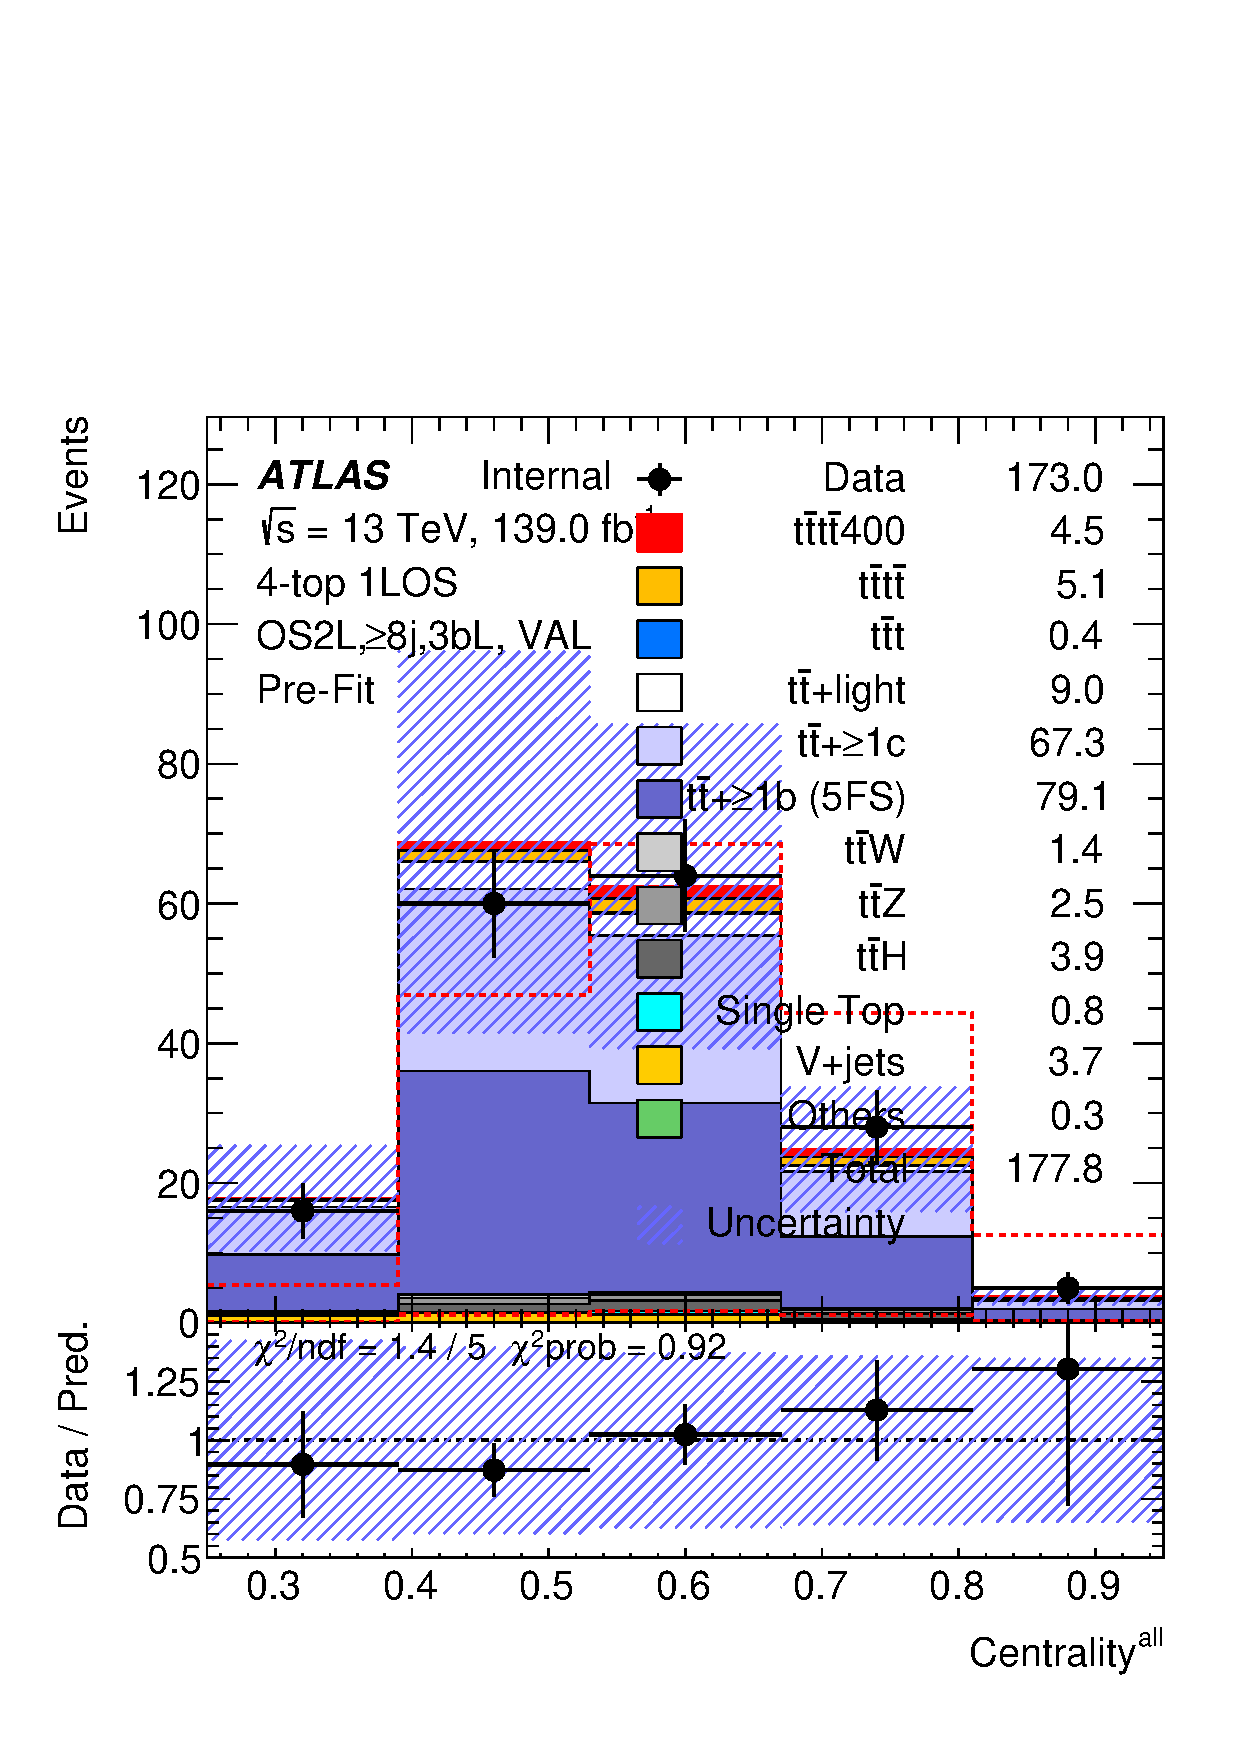
\includegraphics[width=0.23 \textwidth]{figures/fits/GNN/400/all/data_unblindedBonly/Plots/val_os2l_ge8j3bL_centrality.pdf} &
        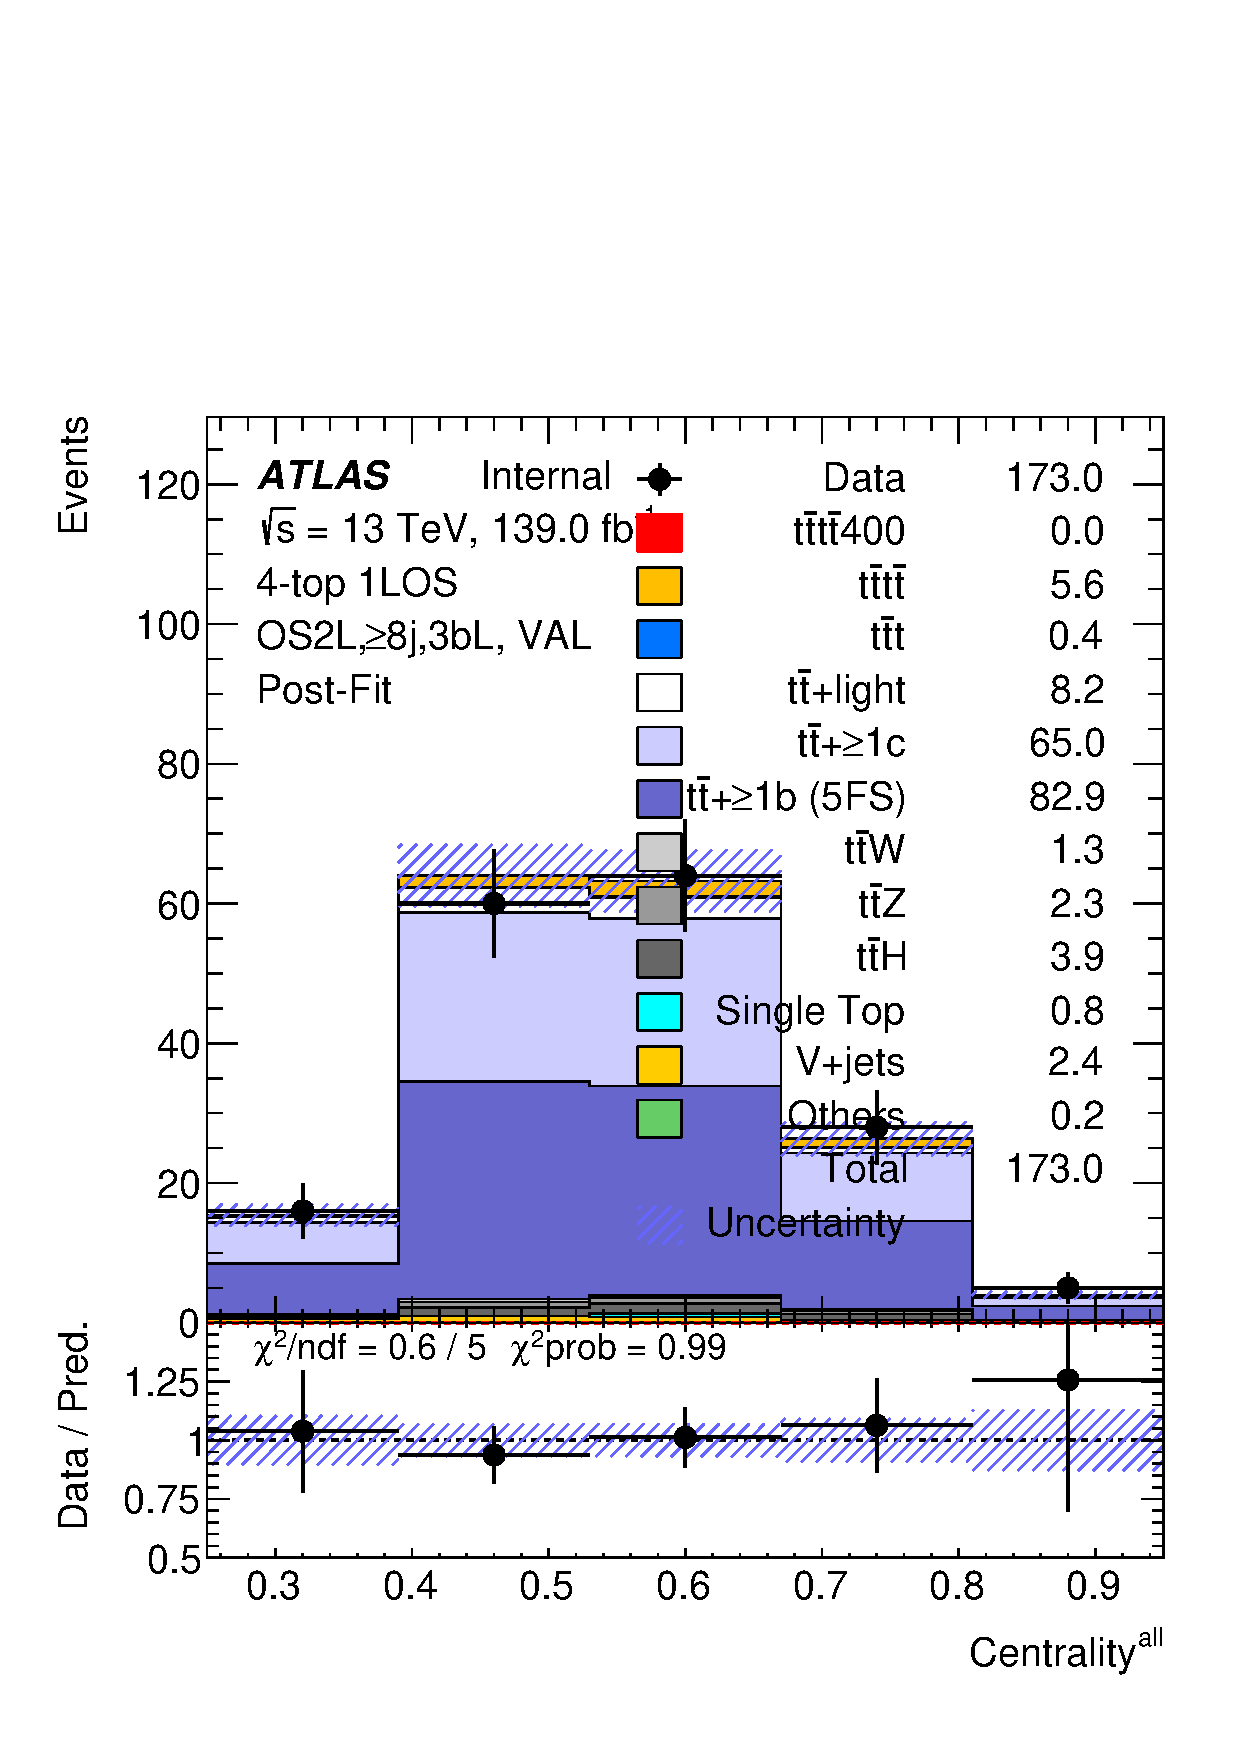
\includegraphics[width=0.23 \textwidth]{figures/fits/GNN/400/all/data_unblindedBonly/Plots/val_os2l_ge8j3bL_centrality_postFit.pdf} &
        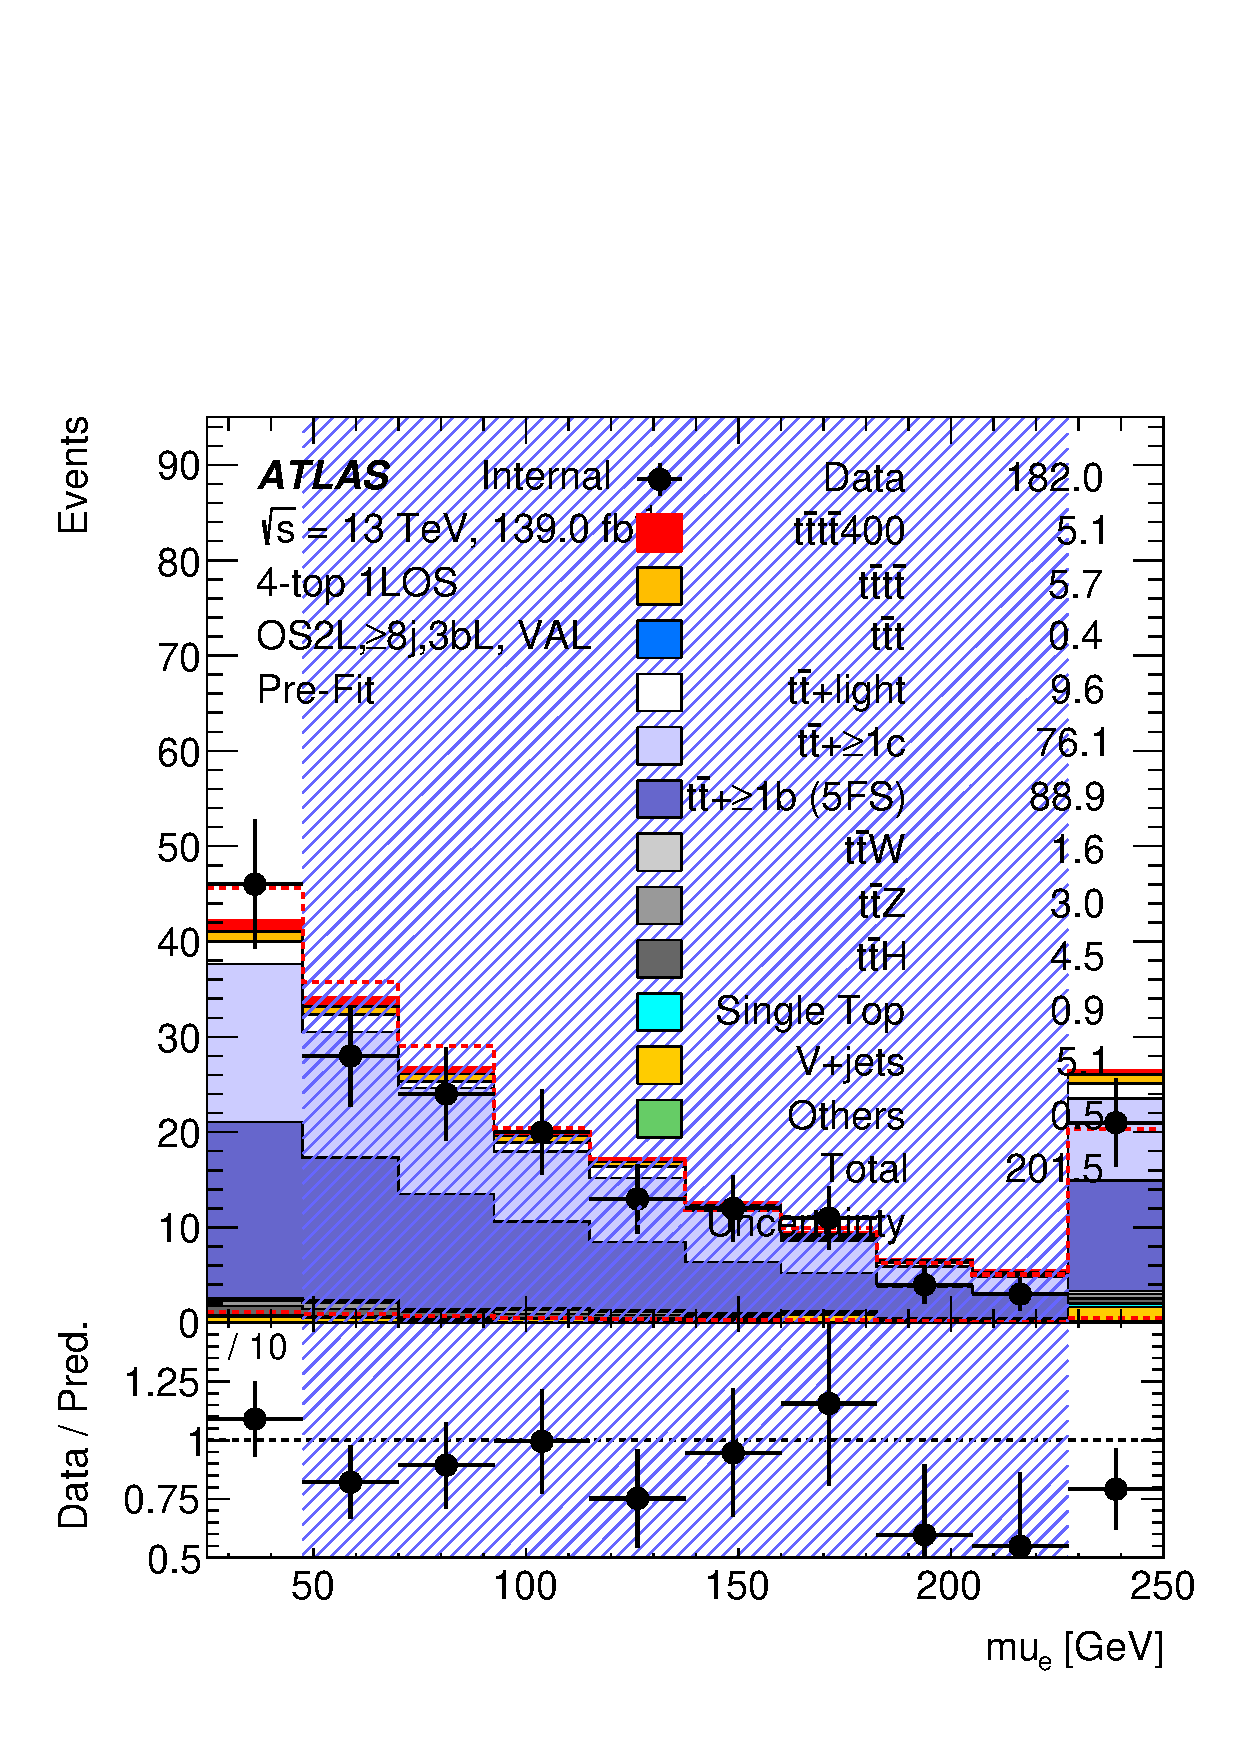
\includegraphics[width=0.23 \textwidth]{figures/fits/GNN/400/all/data_unblindedBonly/Plots/val_os2l_ge8j3bL_mu_e.pdf} &
        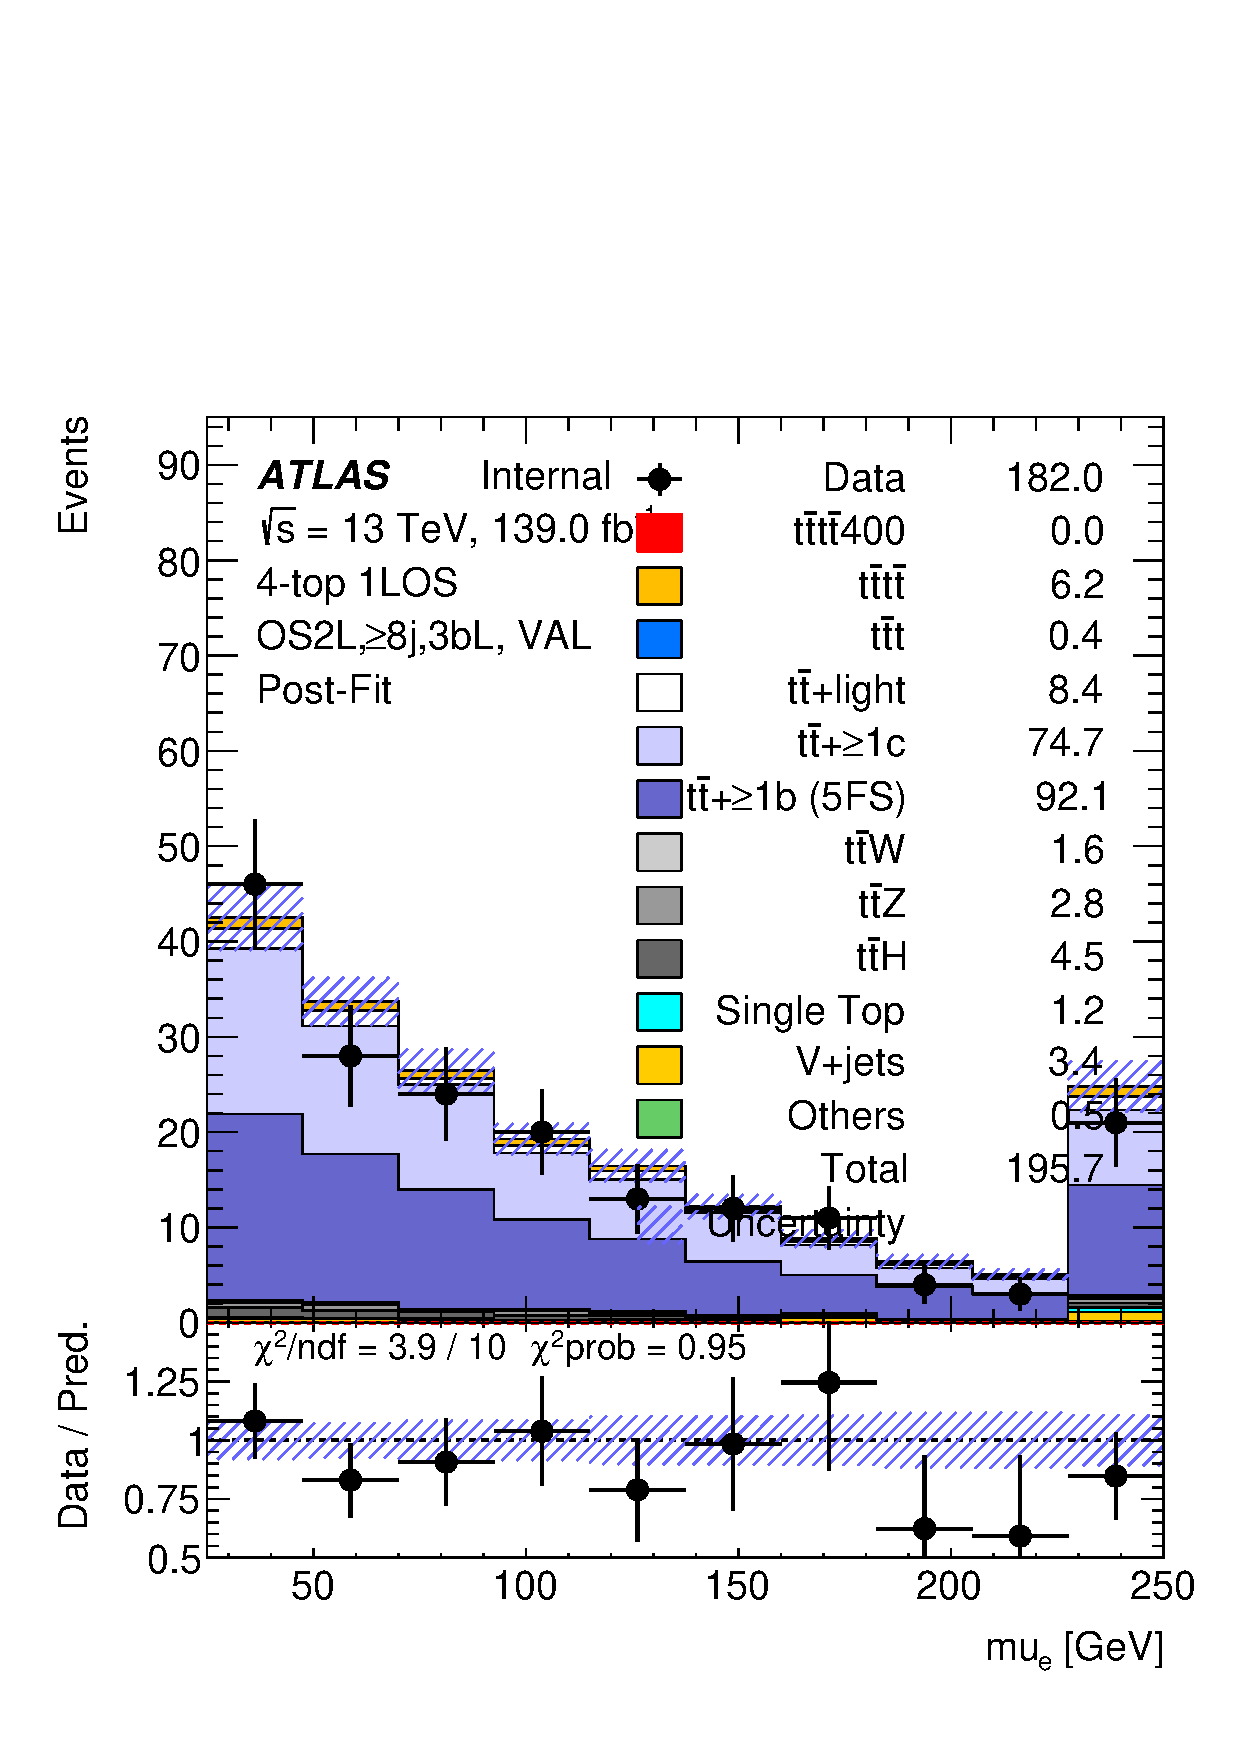
\includegraphics[width=0.23 \textwidth]{figures/fits/GNN/400/all/data_unblindedBonly/Plots/val_os2l_ge8j3bL_mu_e_postFit.pdf} \\

        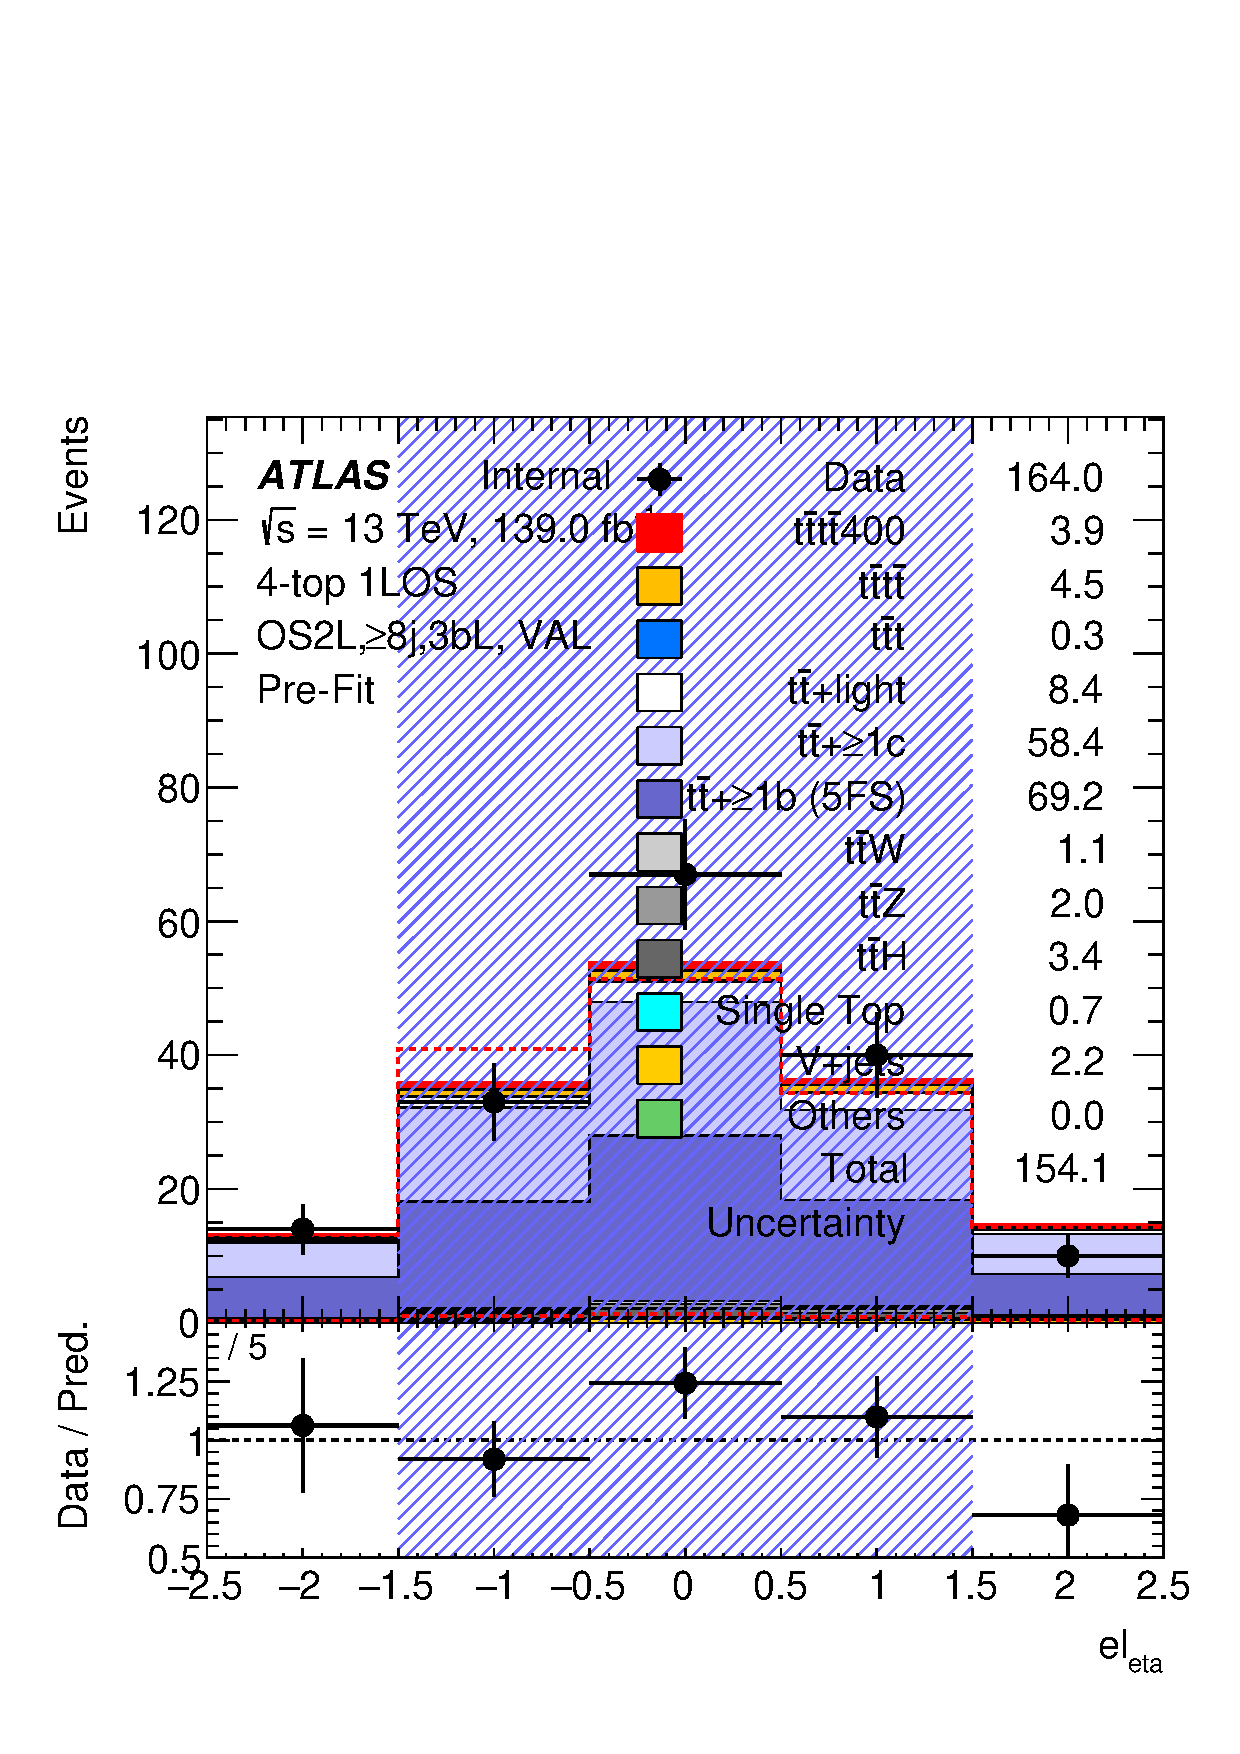
\includegraphics[width=0.23 \textwidth]{figures/fits/GNN/400/all/data_unblindedBonly/Plots/val_os2l_ge8j3bL_mu_eta.pdf} &
        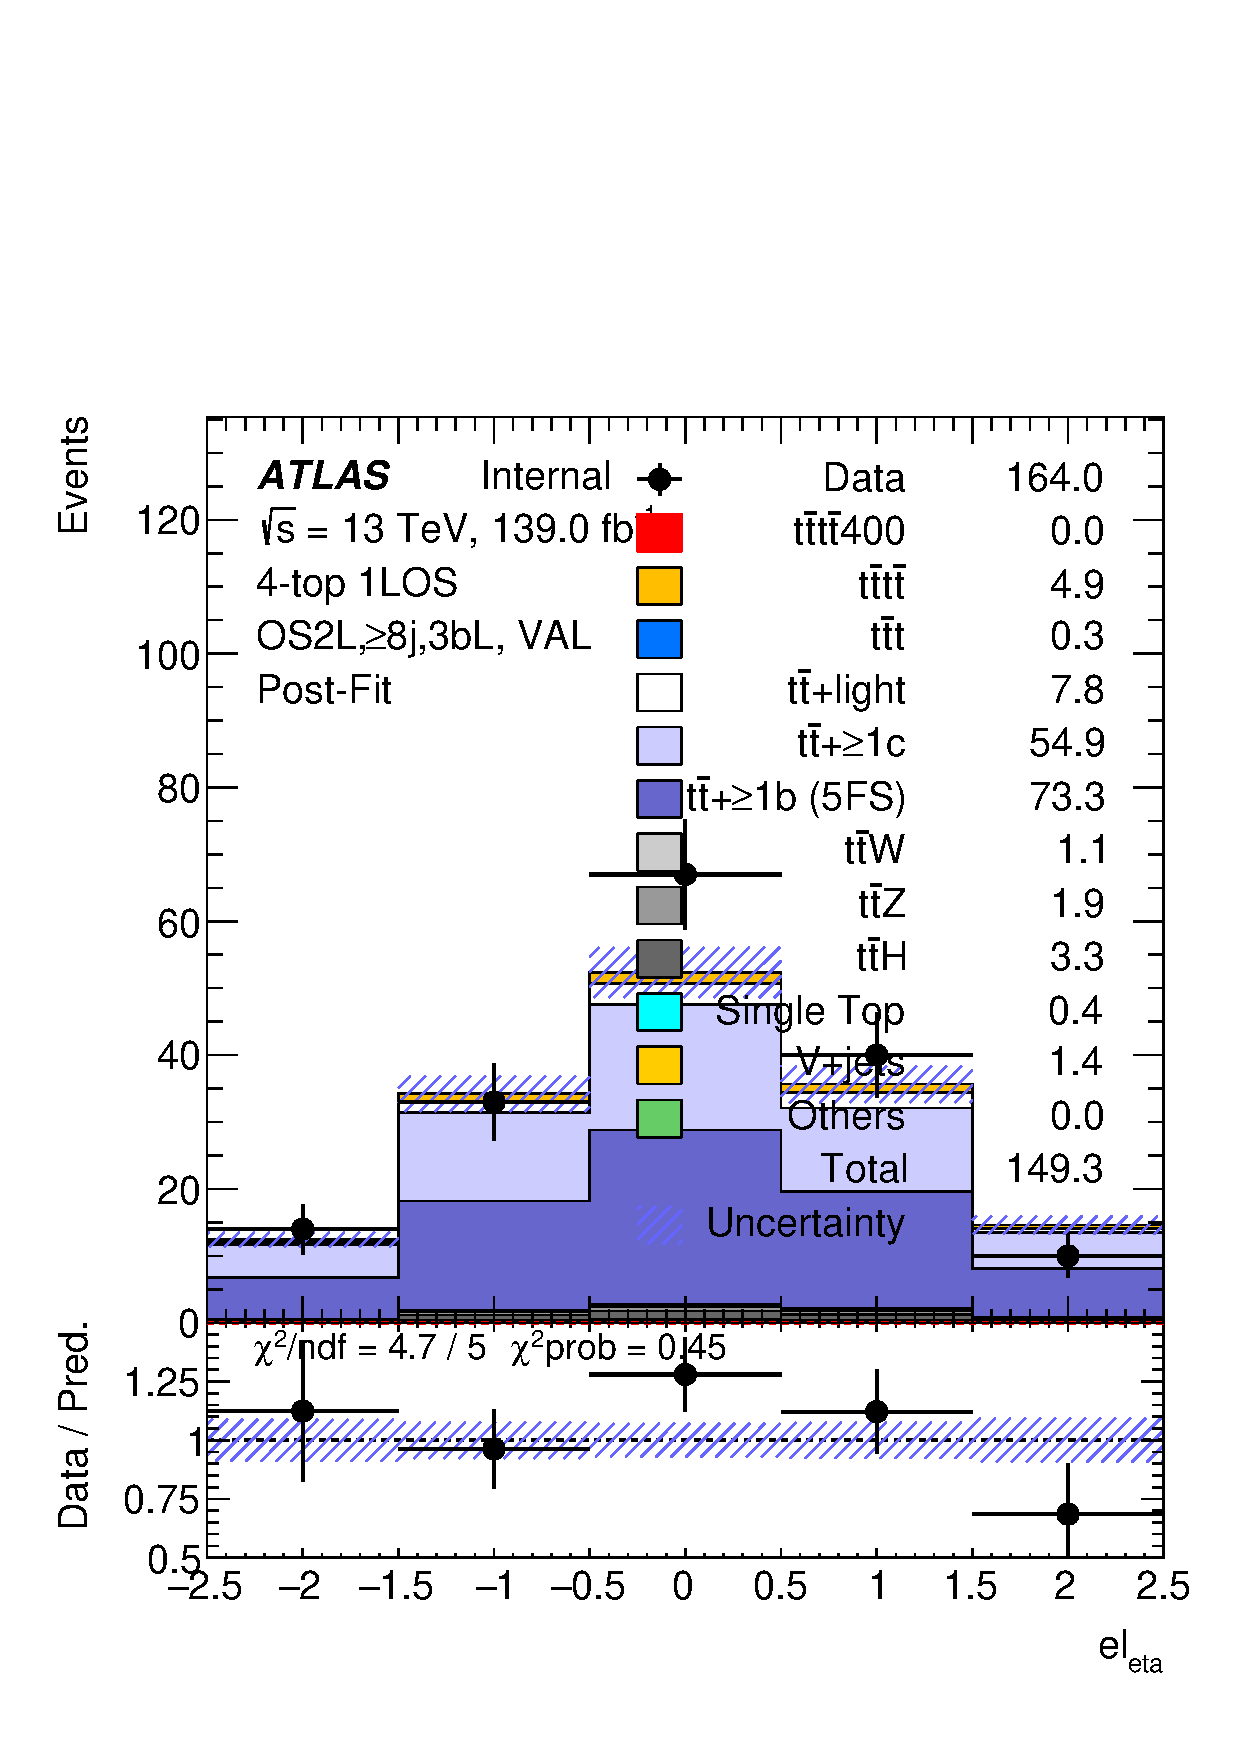
\includegraphics[width=0.23 \textwidth]{figures/fits/GNN/400/all/data_unblindedBonly/Plots/val_os2l_ge8j3bL_mu_eta_postFit.pdf} &
        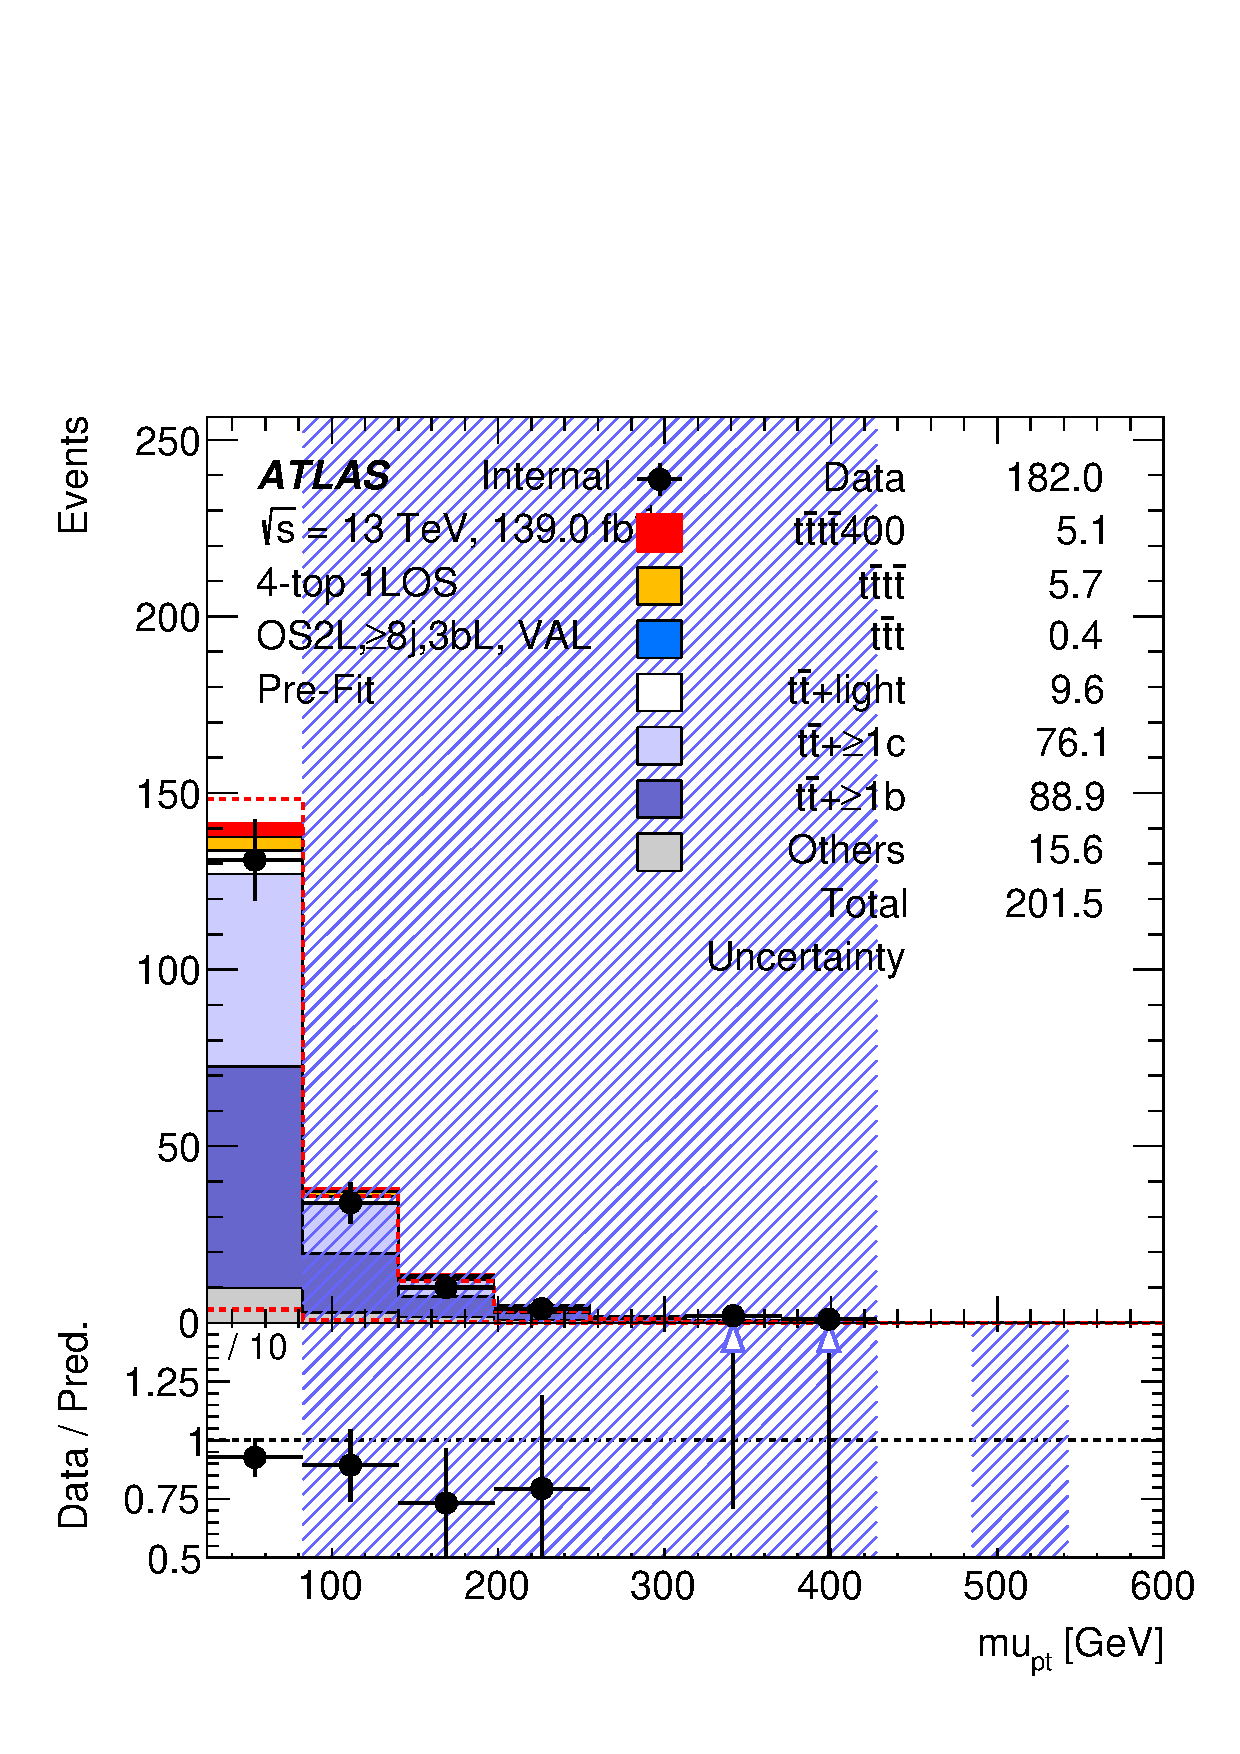
\includegraphics[width=0.23 \textwidth]{figures/fits/GNN/400/all/data_unblindedBonly/Plots/val_os2l_ge8j3bL_mu_pt.pdf} &
        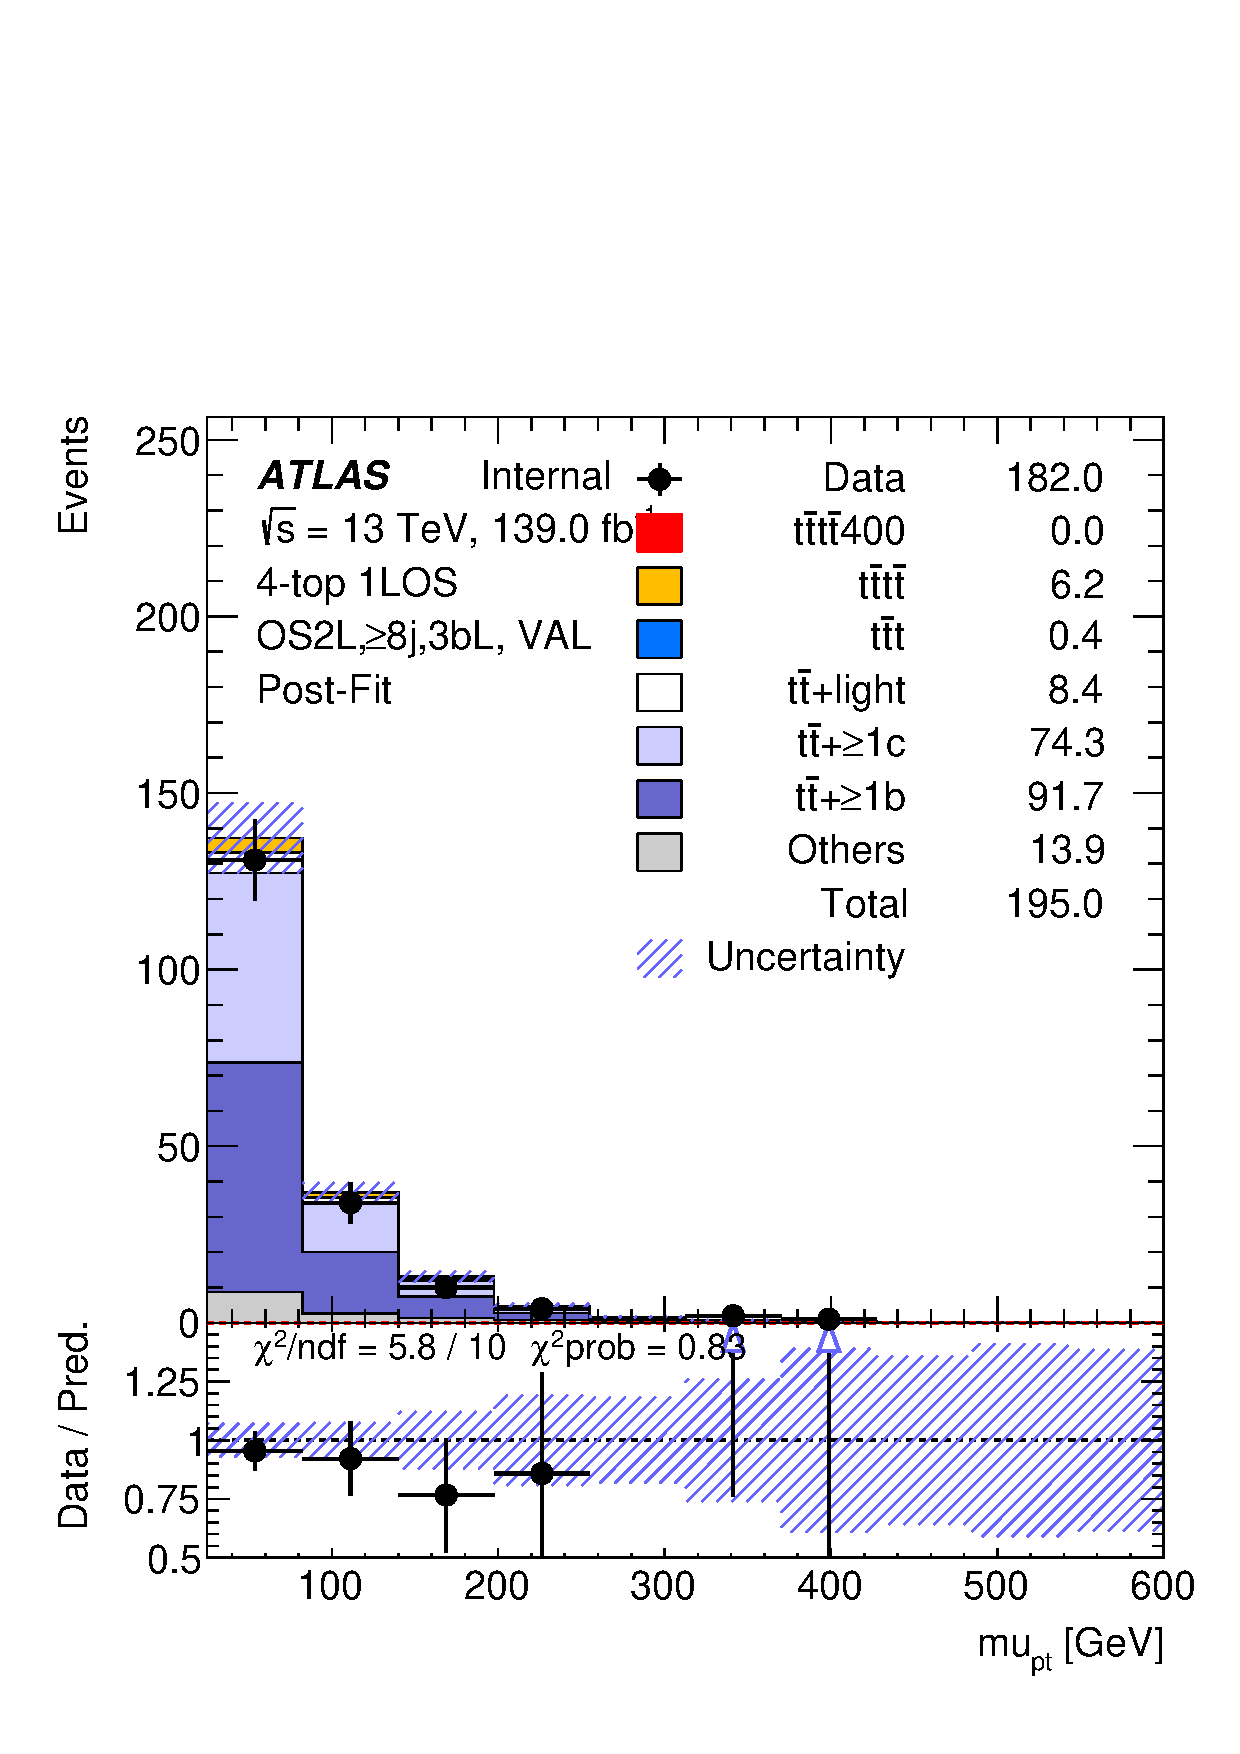
\includegraphics[width=0.23 \textwidth]{figures/fits/GNN/400/all/data_unblindedBonly/Plots/val_os2l_ge8j3bL_mu_pt_postFit.pdf} \\

        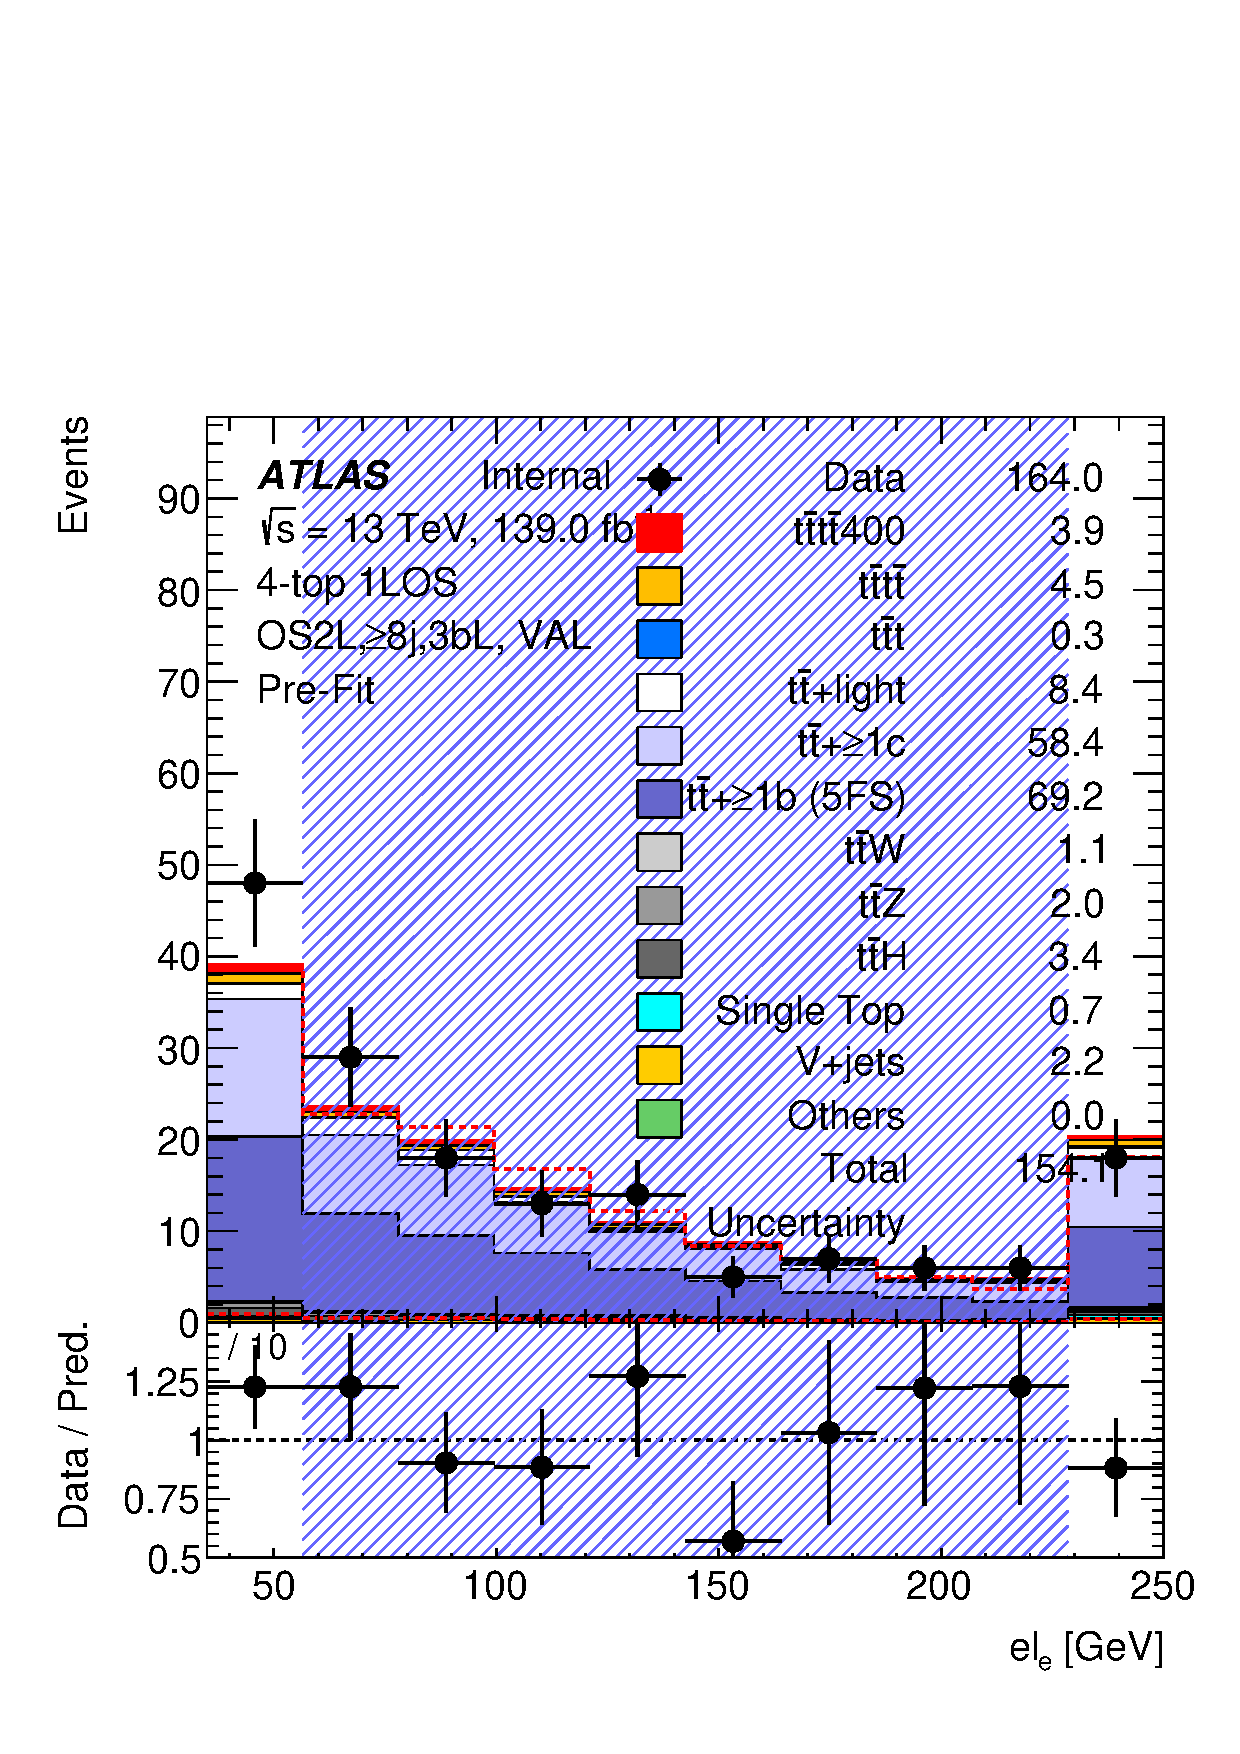
\includegraphics[width=0.23 \textwidth]{figures/fits/GNN/400/all/data_unblindedBonly/Plots/val_os2l_ge8j3bL_el_e.pdf} &
        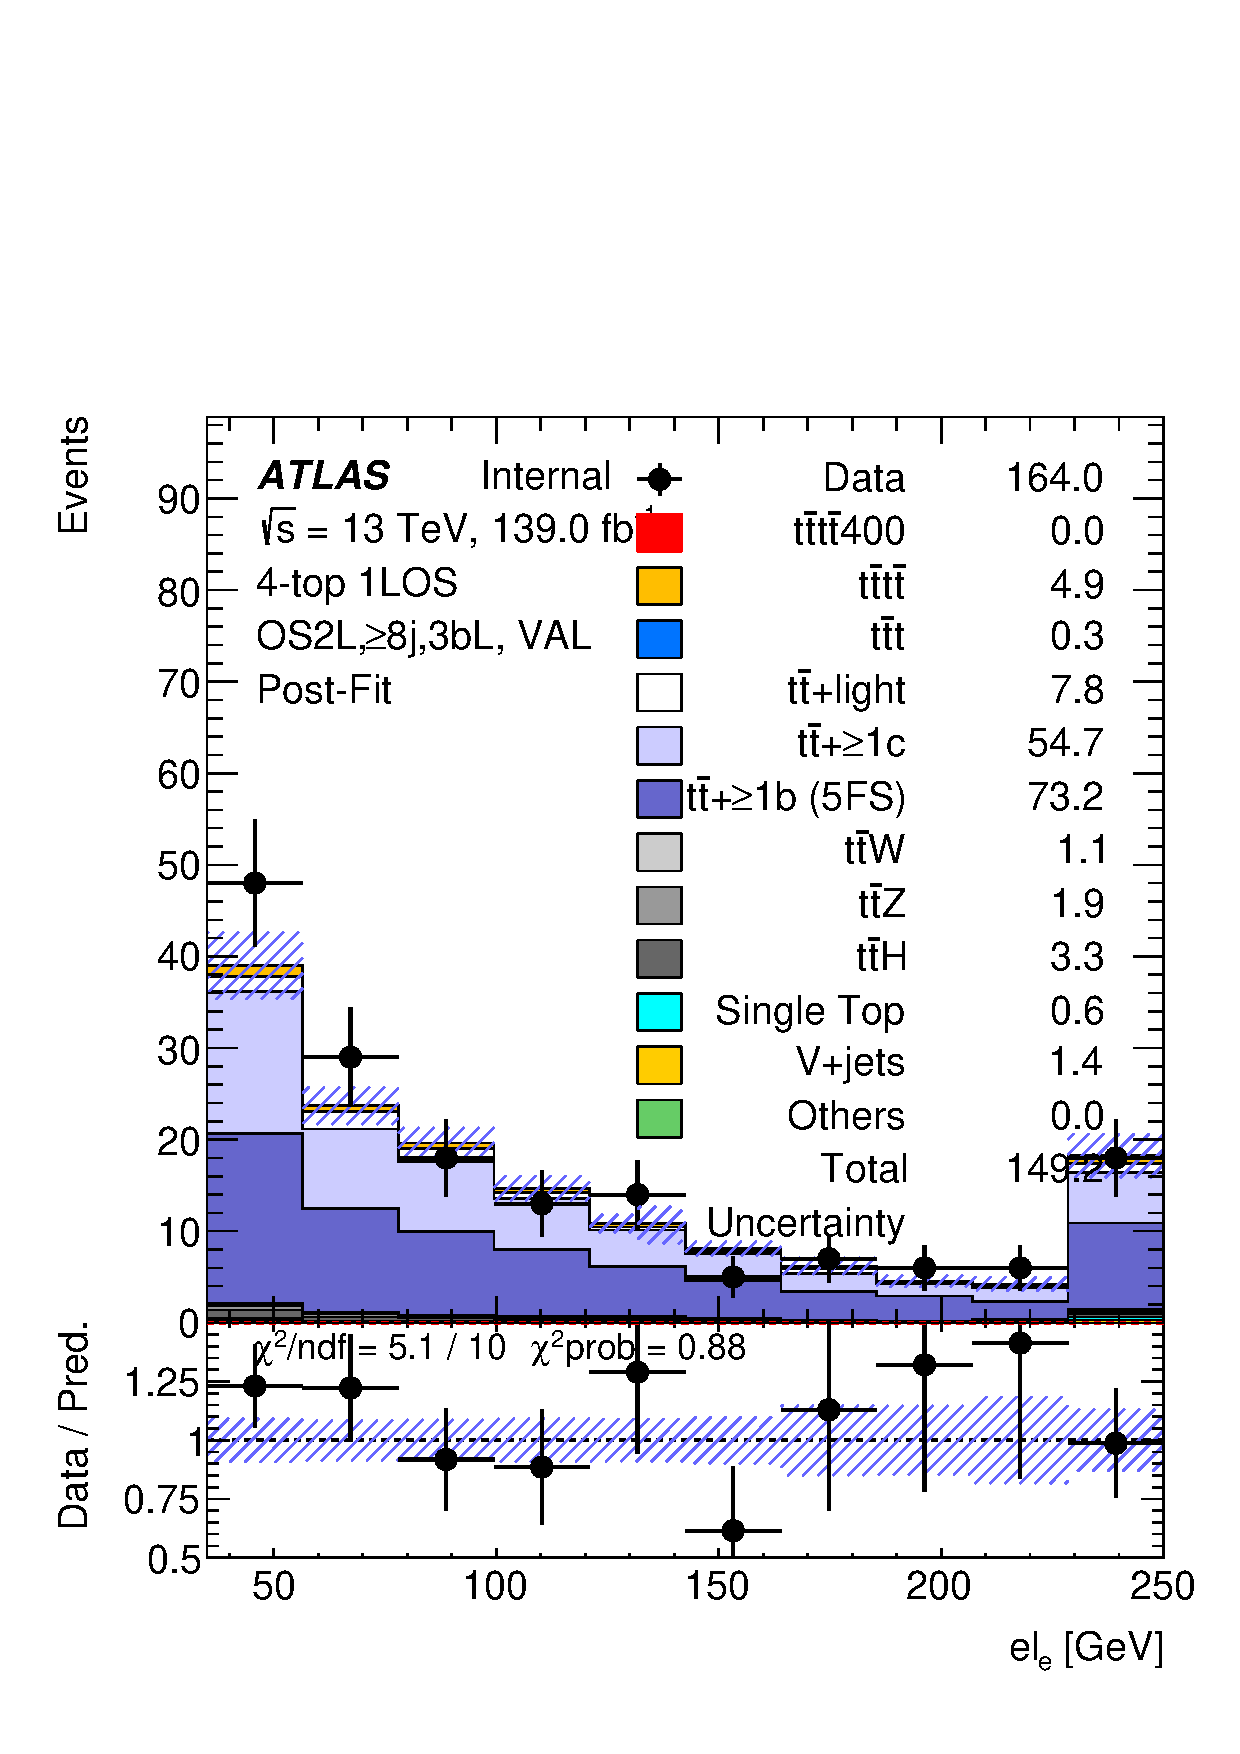
\includegraphics[width=0.23 \textwidth]{figures/fits/GNN/400/all/data_unblindedBonly/Plots/val_os2l_ge8j3bL_el_e_postFit.pdf} &
        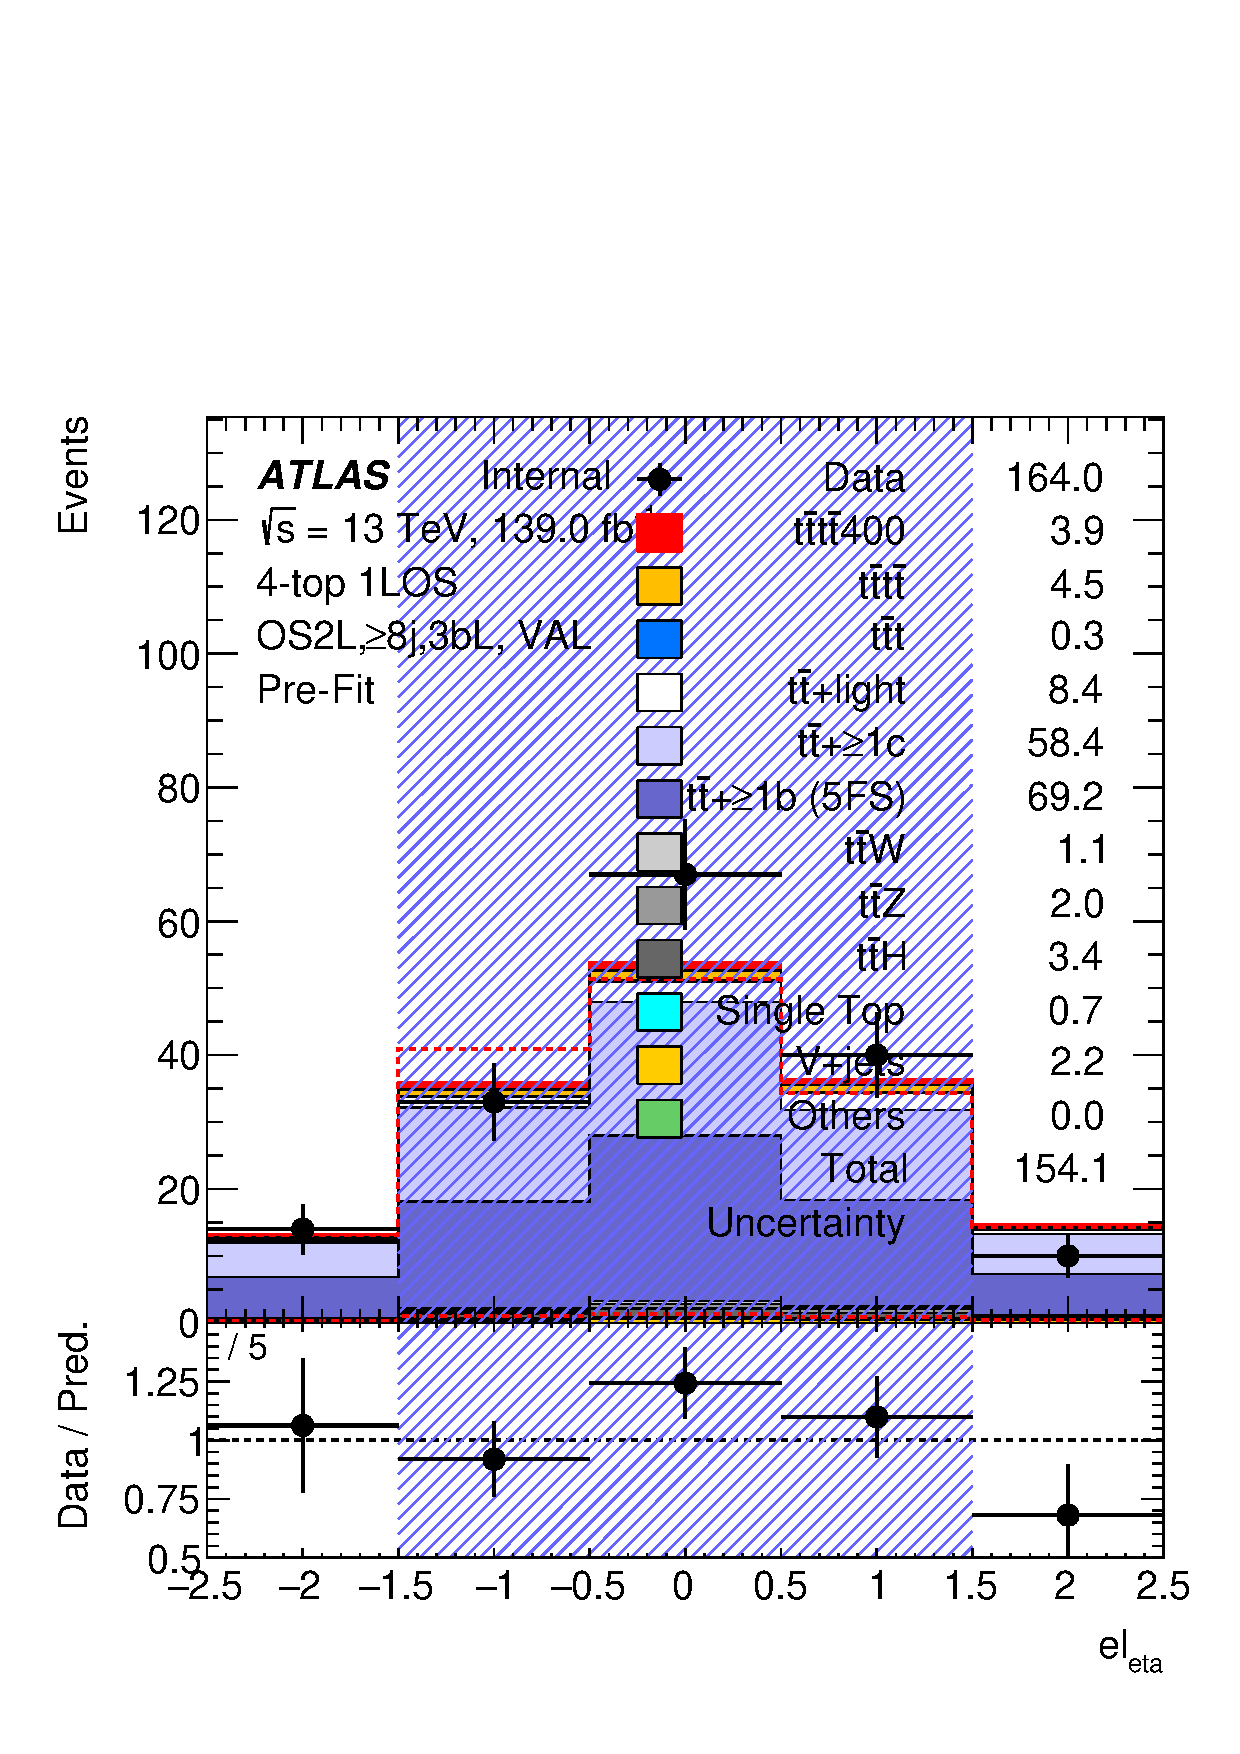
\includegraphics[width=0.23 \textwidth]{figures/fits/GNN/400/all/data_unblindedBonly/Plots/val_os2l_ge8j3bL_el_eta.pdf} &
        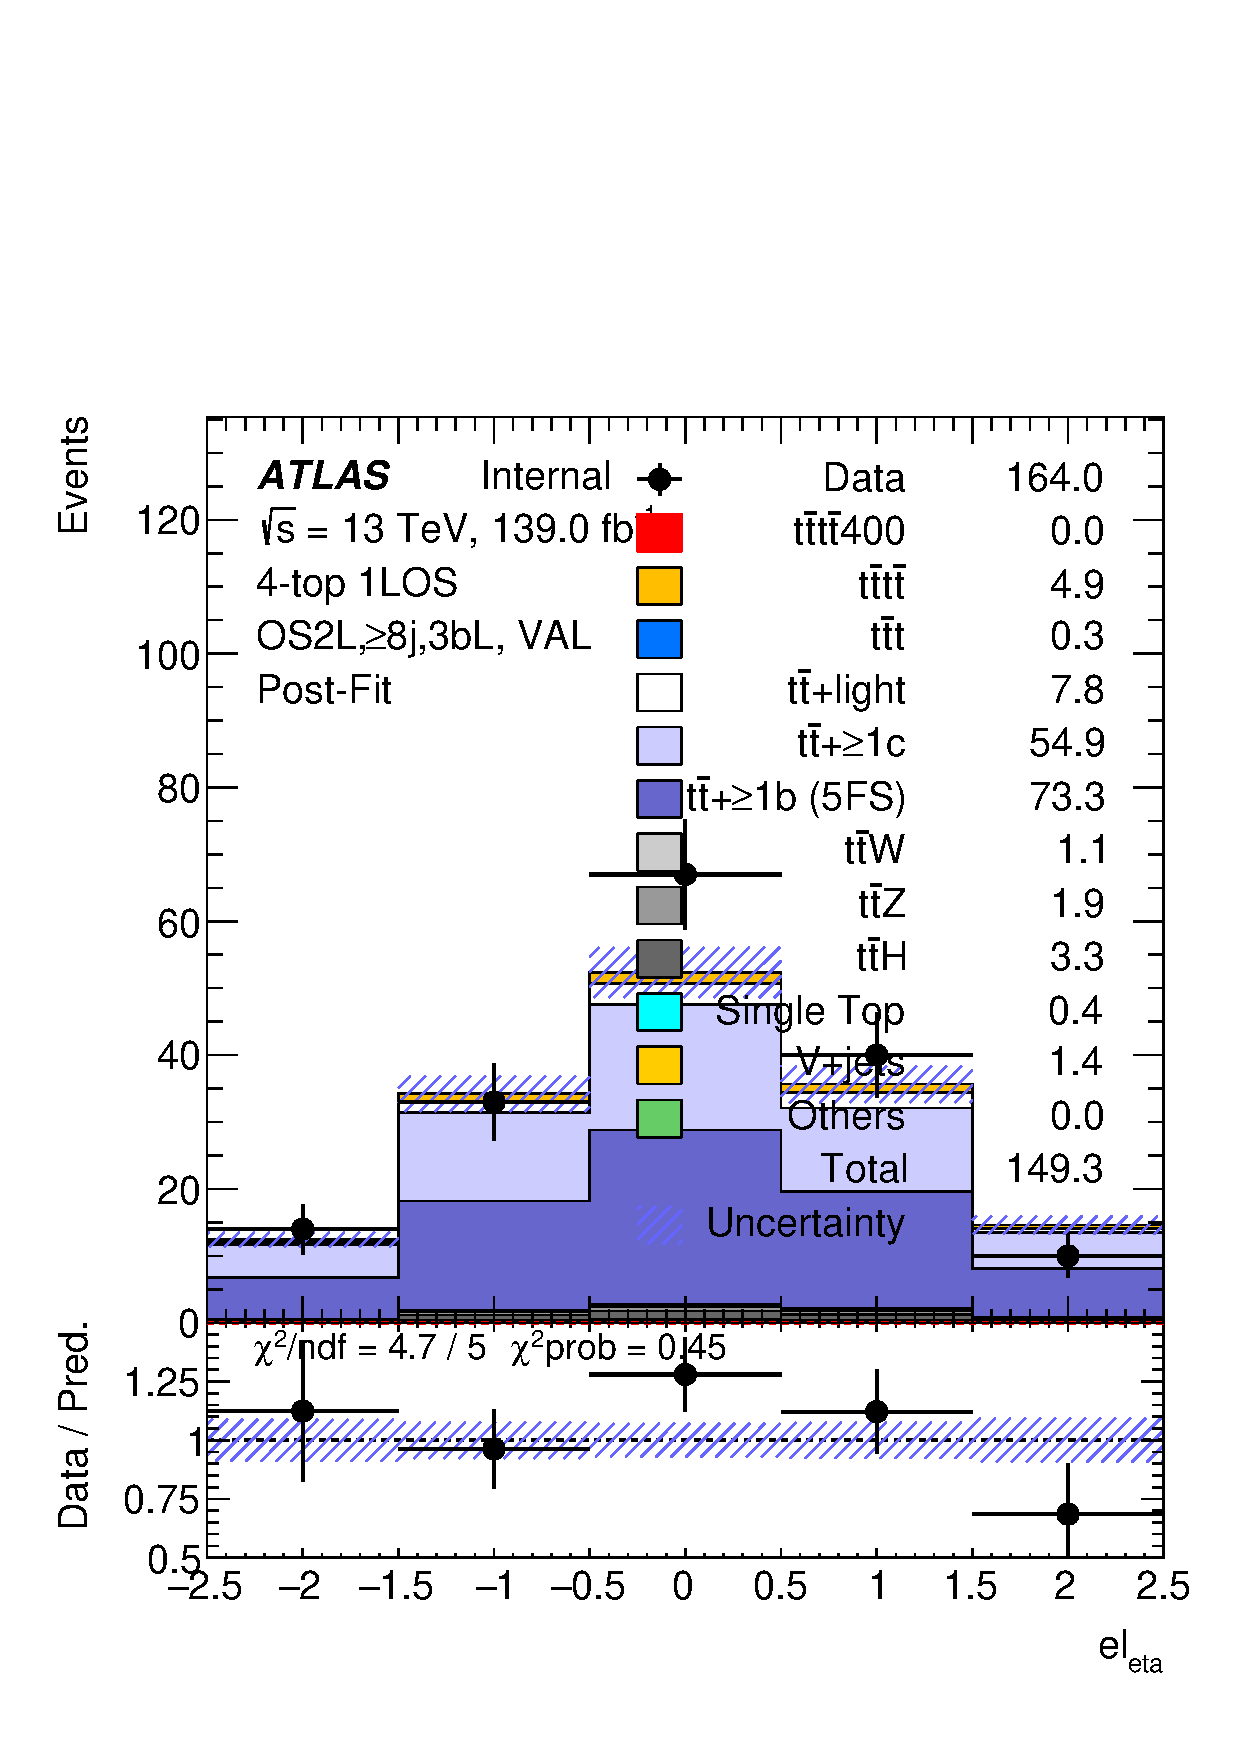
\includegraphics[width=0.23 \textwidth]{figures/fits/GNN/400/all/data_unblindedBonly/Plots/val_os2l_ge8j3bL_el_eta_postFit.pdf} \\

        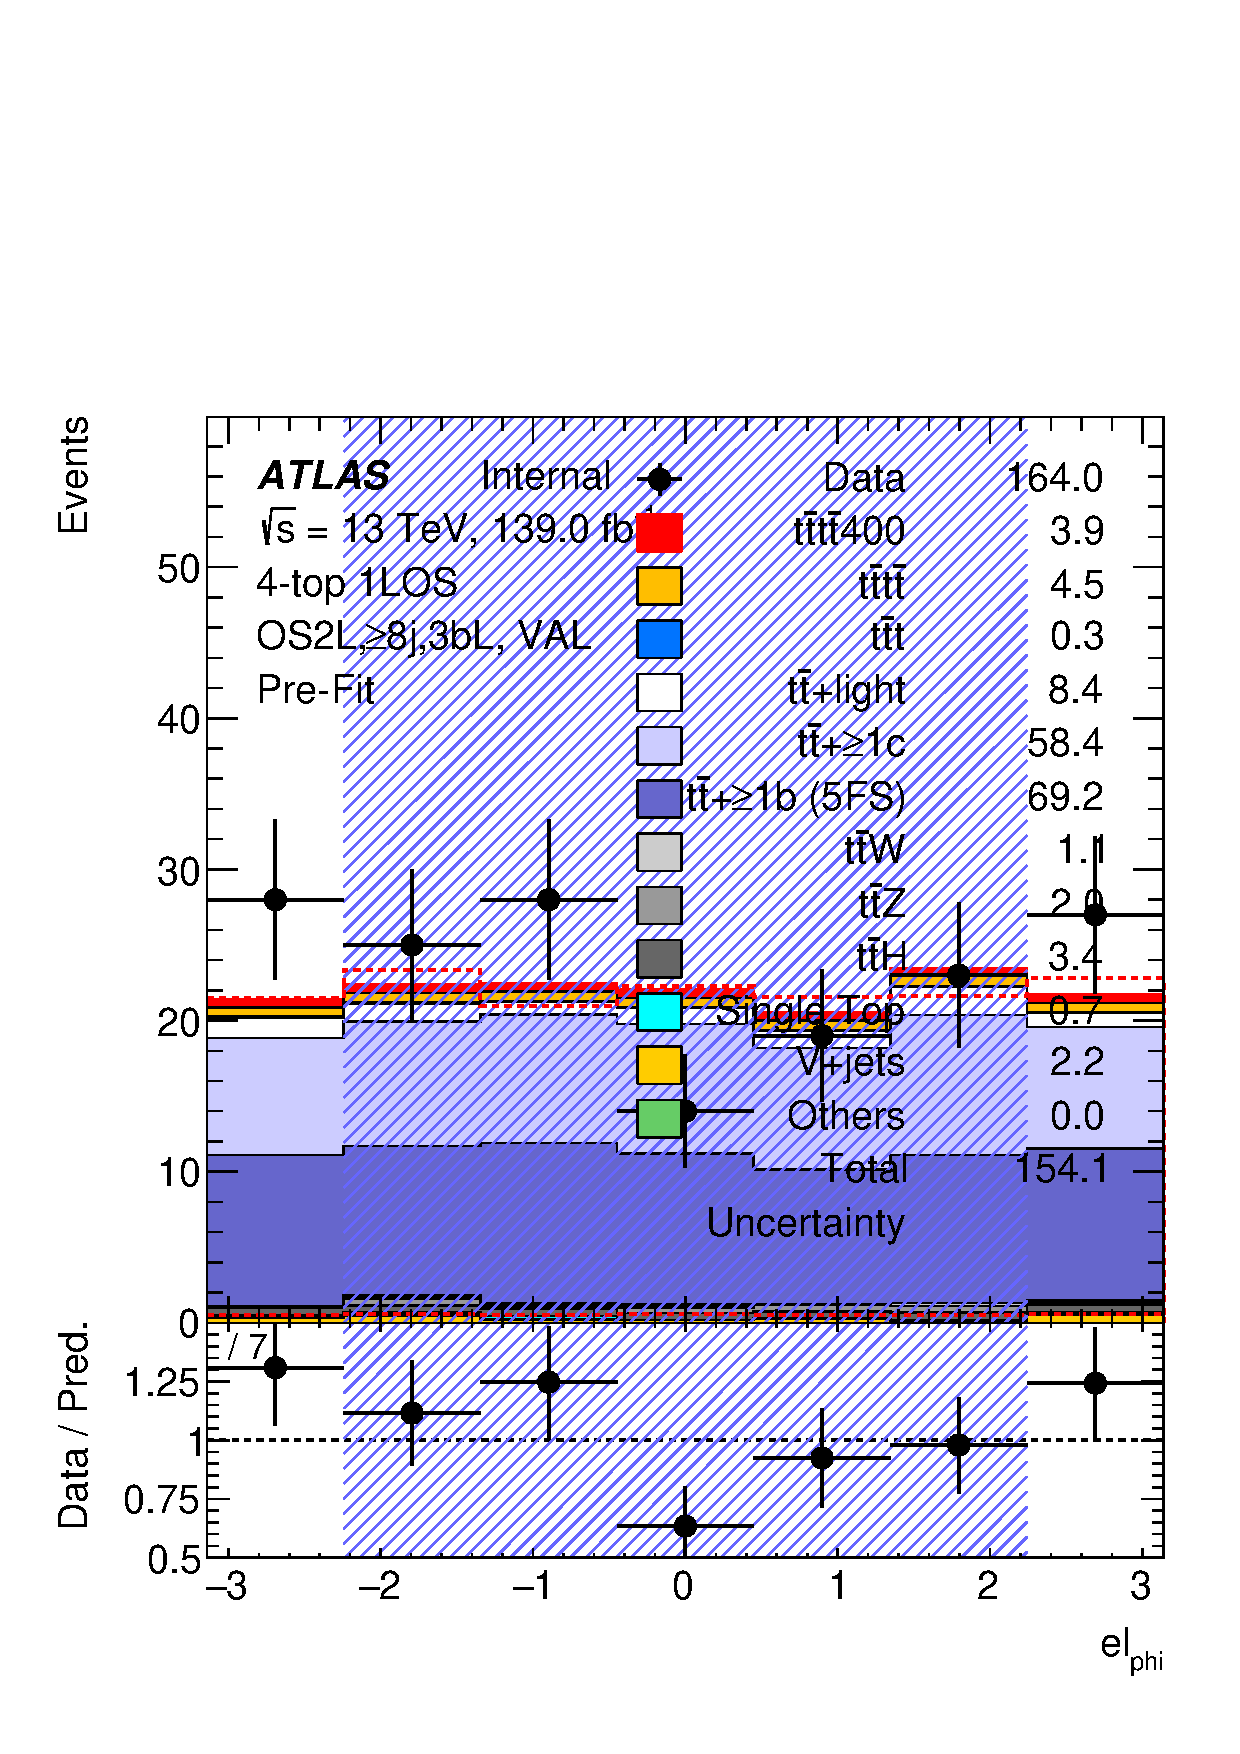
\includegraphics[width=0.23 \textwidth]{figures/fits/GNN/400/all/data_unblindedBonly/Plots/val_os2l_ge8j3bL_el_phi.pdf} &
        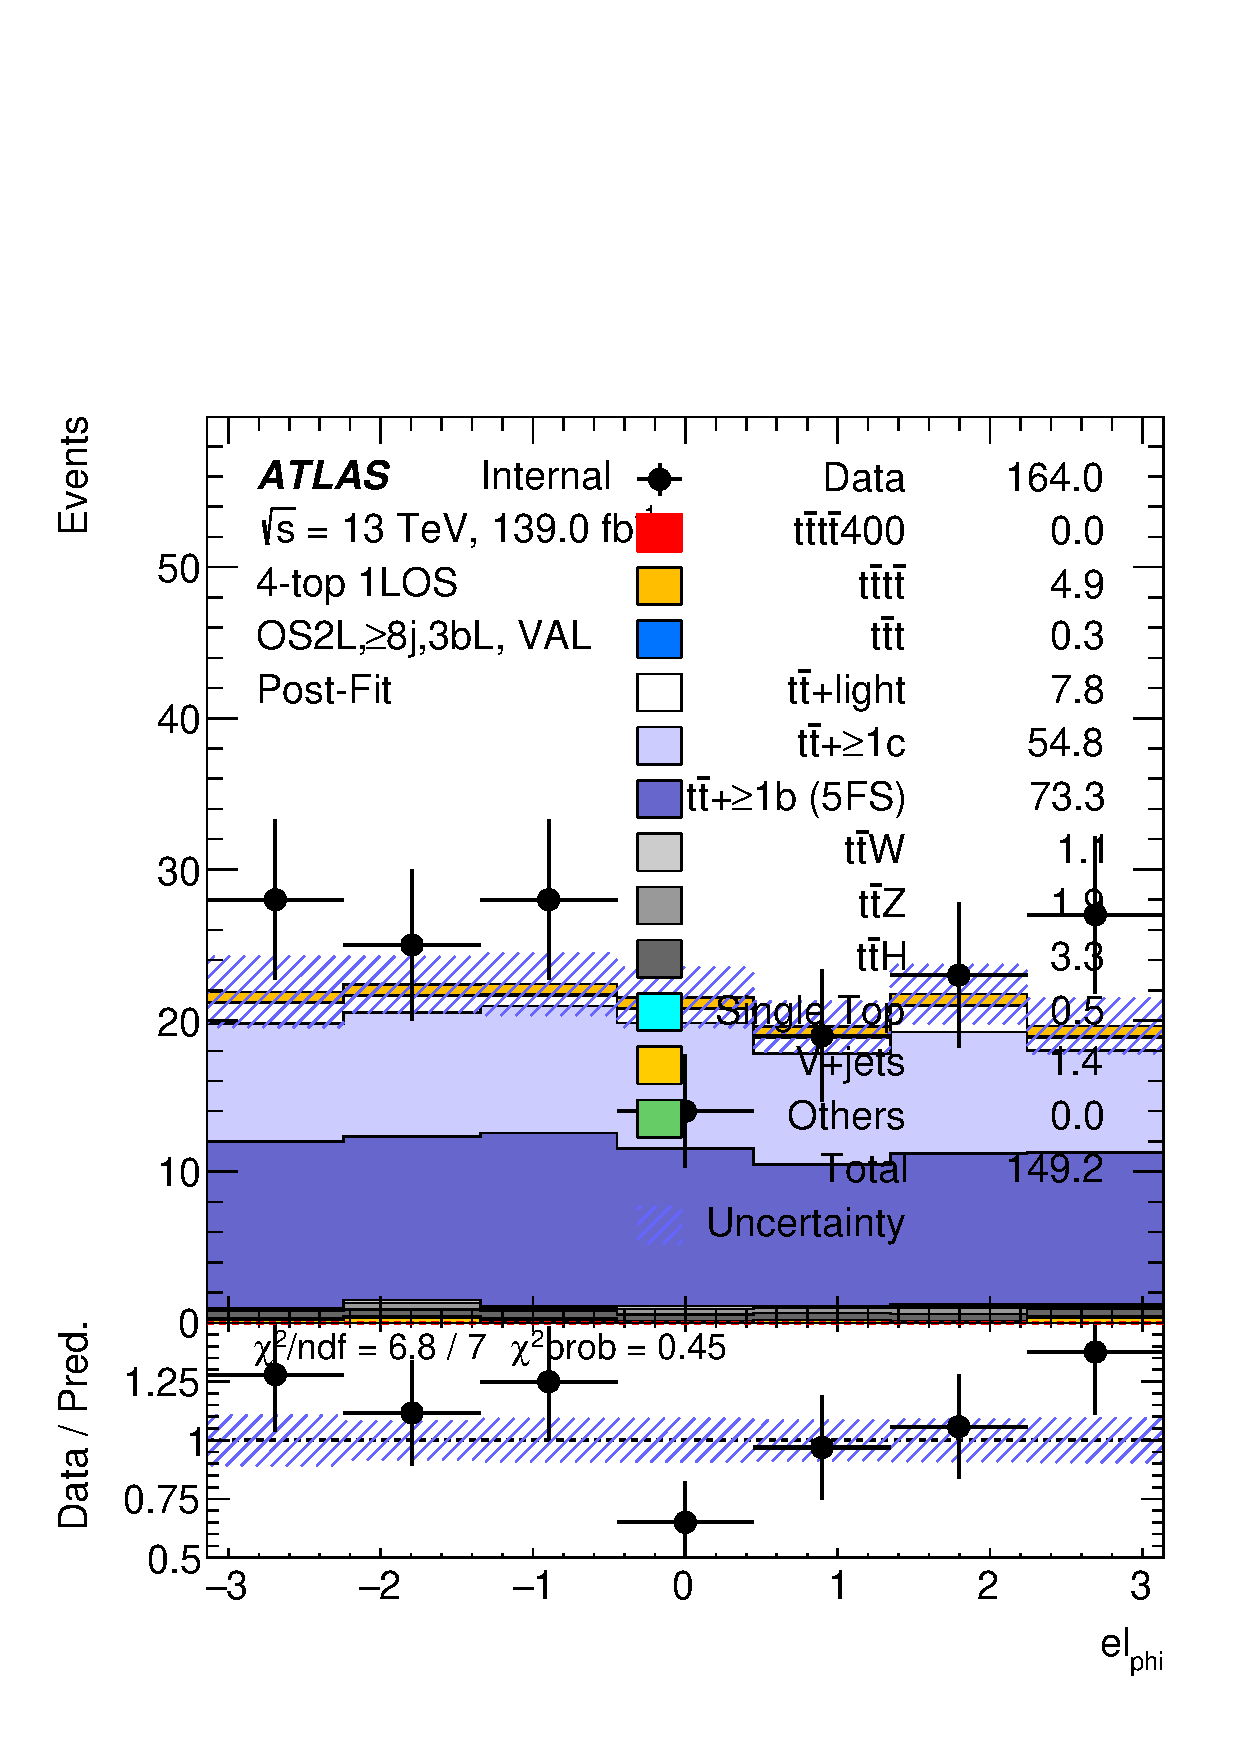
\includegraphics[width=0.23 \textwidth]{figures/fits/GNN/400/all/data_unblindedBonly/Plots/val_os2l_ge8j3bL_el_phi_postFit.pdf} &
        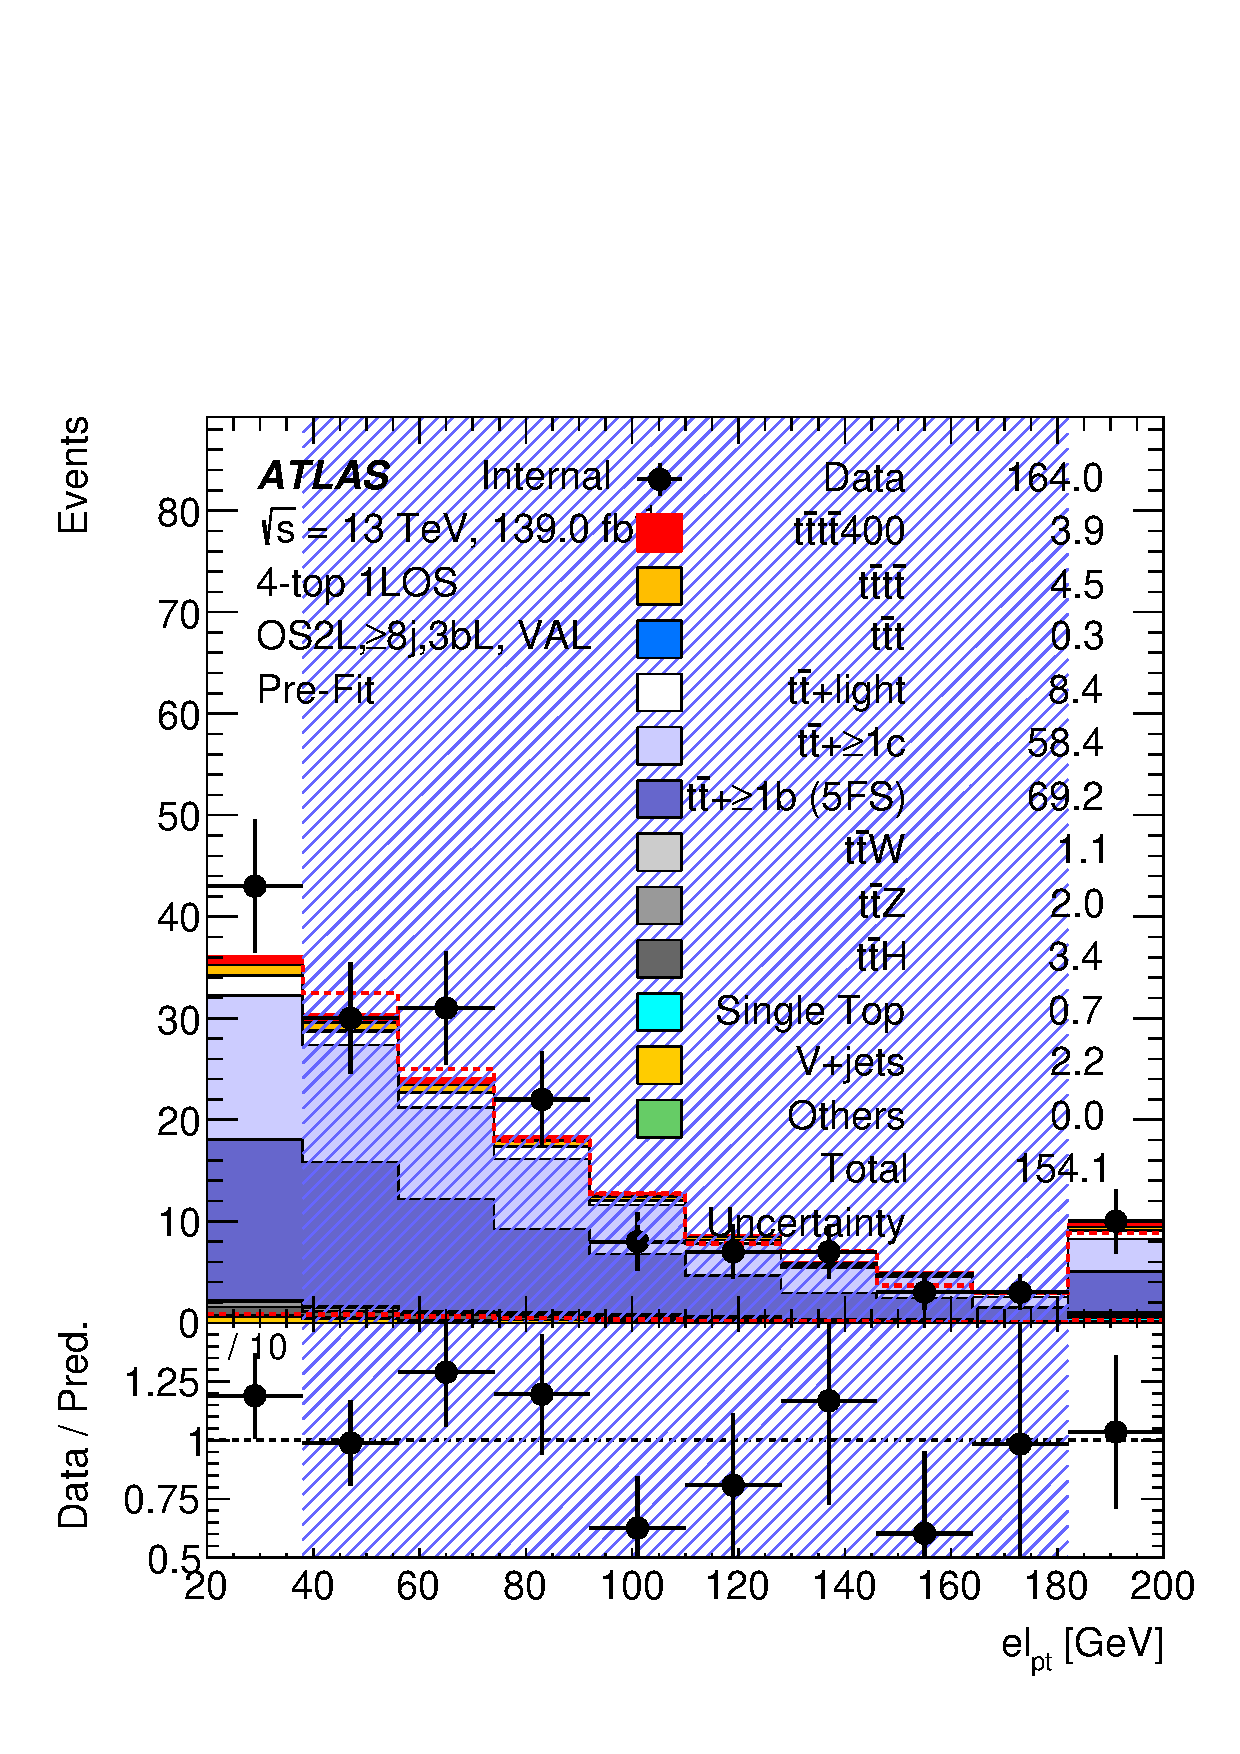
\includegraphics[width=0.23 \textwidth]{figures/fits/GNN/400/all/data_unblindedBonly/Plots/val_os2l_ge8j3bL_el_pt.pdf} &
        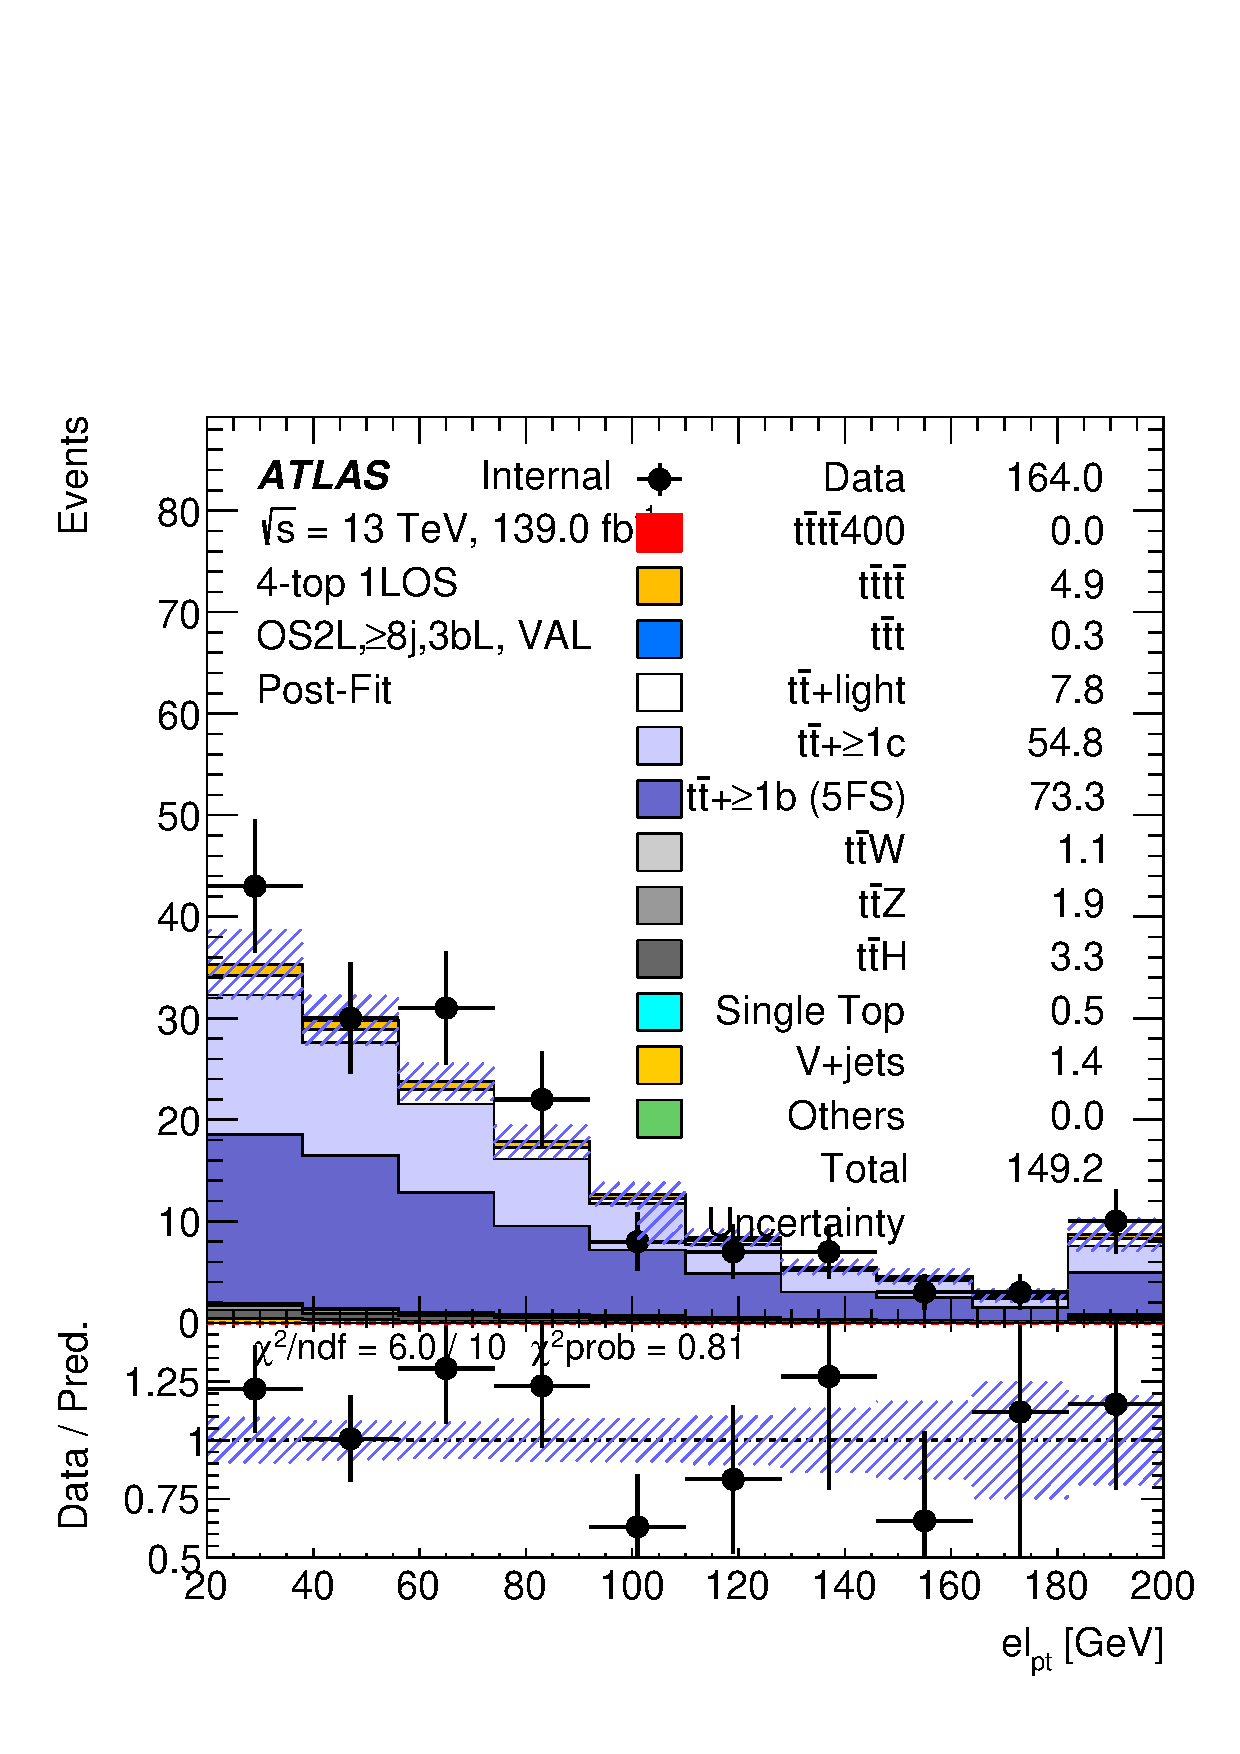
\includegraphics[width=0.23 \textwidth]{figures/fits/GNN/400/all/data_unblindedBonly/Plots/val_os2l_ge8j3bL_el_pt_postFit.pdf} \\
        \end{tabular}
        \end{center}

\caption{\label{GNN_input_val_3}Pre-fit(left) and Post-fit(right) distributions for GNN input variables in the 2L ge8j3bL region.}
\end{figure}



